%%%%%%%%%%%%%%%%%%%%%%%%%%%%%%%%%%%%%%%%
%%% DOCUMENT CLASS AND CLASS OPTIONS %%%
%%%%%%%%%%%%%%%%%%%%%%%%%%%%%%%%%%%%%%%%

% Initial authors:     Michael Enders, Felix Lammermann
% Author's emails:     latex@flammermann.de
%
% Current maintainers: Markus Putnings
% Maintainer's emails: markus.putnings@fau.de
%
%
% Copyright 2019--2020 Michael Enders & Felix Lammermann
% 
% This work may be distributed and/or modified under the conditions of the
% LaTeX Project Public License, either version 1.3c of this license or (at your
% option) any later version.
% 
% The latest version of this license is in
% 
%   http://www.latex-project.org/lppl.txt
% 
% and version 1.3c or later is part of all distributions of LaTeX version
% 2008-05-04 or later.
% 
% This work has the LPPL maintenance status `maintained'.
% The current maintainer of this work is Markus Putnings.

\documentclass[
  paper = 17x24,
  %paper = a5,
    % 17x24 (= studienpartitur, default)
    % a5 (= a5paper)
  language = english,
    % german (= default)
    % english
  acronym = split,
    % none (= false)
    % split (= true, default)
    % combined
    % onlyabbreviation (= nosymbol)
    % onlysymbol (= noabbreviation)
  acronymline = novertical,
    % none (= false)
    % both (= true, all, default)
    % onlyhorizontal (= novertical)
    % onlyvertical (= nohorizontal)
  bibliography = combined,
    % none (= false)
    % split (= true, default)
    % combined
  bibliographypart = all,
    % none (= false)
    % all (= true, default)
    % onlymain
    % nomain
    % onlyown
    % noown
    % onlystudent
    % nostudent
  titlesize = Huge,
    % Huge (= default)
    % LARGE
    % Large
    % large
    % normalsize
  par = halfskip,
    % skip
    % halfskip (= default)
    % indent
]{faupress}


%%%%%%%%%%%%%%%%%%%%%%%%%%%
%%% INDIVIDUAL PACKAGES %%%
%%%%%%%%%%%%%%%%%%%%%%%%%%%
\usepackage{amsmath}
\usepackage{amssymb}
\usepackage{blindtext}
\usepackage{physics}
%\usepackage{bm}
%TODO Best solution so far
\def\bm{\symbf}
%\def\bm{}
\usepackage{relsize}
\usepackage{amsthm}
\theoremstyle{definition}
\newtheorem{theorem}{Theorem}
\newtheorem{definition}{Definition}
\usepackage{caption}
\usepackage{subcaption}
\usepackage{graphicx}
\usepackage{algorithmicx}
\usepackage{algorithm}
\usepackage{algpseudocode}
\usepackage{tikz}
\usepackage{booktabs}
\usepackage{backnaur}
\usepackage{hyperref}
\usepackage[titles]{tocloft}
\usepackage{minted}

% Defs and adaptions
\newcommand{\ps}[1]{\langle #1 \rangle}
\newcommand{\bps}[1]{ \ps{\bm{#1}} }
\newcommand{\state}[3]{( #1 )}
\colorlet{lightred}{red!33}
\colorlet{lightblue}{blue!33}
\renewcommand{\floatpagefraction}{.7}
\renewcommand\theFancyVerbLine{\scriptsize \texttt{\arabic{FancyVerbLine}}}
\numberwithin{equation}{chapter}
\newcounter{prodcounter}
\newenvironment{production}{%
\refstepcounter{prodcounter}
\renewcommand\theequation{p\theprodcounter}
\begin{bnf}}
{\end{bnf}}

\usemintedstyle{tango}
\setminted[python]{fontsize=\footnotesize, breaklines, frame=lines
, numbersep=7.5pt, numberblanklines=False}
\setminted[scala]{fontsize=\footnotesize, breaklines, frame=lines, numbersep=7.5pt, numberblanklines=False}
%\AtBeginDocument{\RenewCommandCopy\qty\SI}
\usepackage{etoolbox}

\AtBeginEnvironment{tabular}{\small}

%%%%%%%%%%%%%%%%%
%%% META INFO %%%
%%%%%%%%%%%%%%%%%

% publication
\title{Automating the Design of Multigrid Methods with Evolutionary Program Synthesis}
\subtitle{Automatisierung des Entwurfs von Mehrgitterverfahren mit Evolutionärer Programmsynthese}

% author
\firstname{Jonas}
\lastname{Schmitt}
%\degree{M.Sc.}
\origin{Forchheim}

% publication identifiers
\yearofpublication{2022}
\series{}
\volume{}
\doi{}
\isbn{}
\eisbn{}
\issn{}
\printinformation{%
%  ggf. Satz \\%
%  ggf. Druck%
}

% miscellaneous
\subject{Doktorarbeit}
\keywords{FAU, Erlangen, Nürnberg, Doktorarbeit}

% university and examination
\institute{Lehrstuhl für Informatik 10}
\supervisor{Prof. Dr. Harald Köstler}
\oralexam{}
\dean{}
\reviewer{Prof. Dr. Harald Köstler \\ 
Prof. Dr. Penousal Machado \\
Prof. Dr. Dietmar Fey}


%%%%%%%%%%%%%%%%%%%%%%%%%
%%% DOCUMENT CONTENTS %%%
%%%%%%%%%%%%%%%%%%%%%%%%%

\begin{document}

% typeset the titlepage of the publisher
%\maketitle

% start the frontmatter (roman page numbering,
% lowercase roman sectioning numbering, no header)
\frontmatter
  
  % typesets the titlepage of the faculty
  \makefacultytitle

  % insert preface heading (has \label{ch:preface},
  % reference via \nameref{ch:preface})
  \begin{abstract}
    Many of the most fundamental laws of nature can be formulated as partial differential equations (PDEs). 
Understanding these equations is, therefore, of exceptional importance for many branches of modern science and engineering. 
However, since the general solution of many PDEs is unknown, the efficient approximate solution of these equations is one of humanity's greatest challenges.
While multigrid represents one of the most effective methods for solving PDEs numerically, in many cases, the design of an efficient or at least working multigrid solver is an open problem.
This thesis demonstrates that grammar-guided genetic programming, an evolutionary program synthesis technique, can discover multigrid methods of unprecedented structure that achieve a high degree of efficiency and generalization.
For this purpose, we develop a novel context-free grammar that enables the automated generation of multigrid methods in a symbolically-manipulable formal language, based on which we can apply the same multigrid-based solver to problems of different sizes without having to adapt its internal structure.
Treating the automated design of an efficient multigrid method as a program synthesis task allows us to find novel sequences of multigrid operations, including the combination of different smoothing and coarse-grid correction steps on each level of the discretization hierarchy.
To prove the feasibility of this approach, we present its implementation in the form of the Python framework EvoStencils, which is freely available as open-source software.
This implementation comprises all steps from representing the algorithmic sequence of a multigrid method in the form of a directed acyclic graph of Python objects to its automatic generation and optimization using the capabilities of the code generation framework ExaStencils and the evolutionary computation library DEAP.
We furthermore describe how this implementation can be extended to yield multigrid methods that can efficiently solve multiple instances of the same PDE, thus achieving strong generalizability.
Even though generalization is one of the main goals of automated solver generation, artificial intelligence-based methods often fail to achieve it. 
While machine learning models have shown promise in replacing classical numerical solvers, they typically rely on a fixed-size neural network and can thus not easily be generalized to other problem sizes.
To speed up the evaluation of a large number of multigrid-based solvers, we derive a suitable distributed parallelization scheme based on the message-passing interface (MPI) that allows EvoStencils to leverage the computational power of modern clusters and supercomputers.
To investigate the effectiveness of our approach, we consider several different PDEs, including the indefinite Helmholtz equation, for which we obtain multigrid methods that achieve superior solving efficiency compared to classical multigrid cycles.
Moreover, some of the methods discovered with our approach are able to achieve convergence in the case of an extremely ill-conditioned Helmholtz problem, for which, at the same time, all known multigrid cycles fail to yield a converging solver.
Within our experiments, we also show that our implementation can be executed on recent clusters and supercomputers, such as SuperMUC-NG, currently one of Europe's largest supercomputing systems.
Finally, since our formal representation of multigrid methods can easily be translated into a human-readable format, we also perform an empirical analysis of the algorithmic features discovered with our evolutionary program synthesis approach.
  \end{abstract}
  \begin{zusammenfassung}
    Viele der grundlegendsten Naturgesetze können als partielle Differentialgleichungen (PDGs) formuliert werden. 
Das Verständnis dieser Gleichungen ist daher für viele Bereiche der modernen Wissenschaft und Technik von immenser Bedeutung. 
Da jedoch die allgemeine Lösung vieler PDGs unbekannt ist, stellt die effiziente Näherungslösung dieser Gleichungen eine der größten Herausforderungen der Menschheit dar.
Obwohl Mehrgitterverfahren eine der effektivsten Methoden zur numerischen Lösung von PDGs darstellen, ist der Entwurf eines effizienten oder zumindest funktionierenden Mehrgitterlösers in vielen Fällen ein offenes Problem.
In dieser Arbeit wird gezeigt, dass grammatikgeleitete genetische Programmierung, eine evolutionäre Programmsynthesetechnik, zur Entdeckung von Mehrgitterverfahren bisher unerreichter Struktur führen kann, welche zudem einen hohen Grad an Effizienz und Generalisierung erreichen.
Zu diesem Zweck entwickeln wir eine neuartige kontextfreie Grammatik, welche die automatisierte Generierung von Mehrgitterverfahren in einer symbolisch manipulierbaren formalen Sprache ermöglicht, auf deren Grundlage wir denselben mehrgitterbasierten Löser auf Probleme unterschiedlicher Größe anwenden können, ohne seine interne Struktur anpassen zu müssen.
Die Behandlung des automatisierten Entwurfs effizienter Mehrgitterverfahren als Programmsyntheseproblem erlaubt es uns neuartige Sequenzen von Mehrgitteroperationen zu finden, einschließlich der Kombination von verschiedenen Glättungs- und Grobgitterkorrekturschritten auf jeder Ebene der Diskretisierungshierarchie.
Um die Machbarkeit dieses Ansatzes zu beweisen, stellen wir seine Implementierung in Form des Python-Frameworks EvoStencils vor, das als Open-Source-Software frei verfügbar ist.
Diese Implementierung umfasst alle Schritte von der Darstellung der algorithmischen Sequenz eines Mehrgitterverfahrens in Form eines gerichteten azyklischen Graphen bestehend aus Python-Objekten bis hin zu seiner automatischen Generierung und Optimierung unter Verwendung der Fähigkeiten des ExaStencils-Frameworks zur Codegenerierung und der Bibliothek DEAP für die Implementierung evolutionärer Algorithmen.
Darüber hinaus beschreiben wir, wie diese Implementierung erweitert werden kann, um Mehrgittermethoden zu erhalten, die mehrere Instanzen derselben PDG effizient lösen können, wodurch eine starke Generalisierbarkeit erreicht werden kann.
Obwohl die Verallgemeinerung eines der Hauptziele bei der automatischen Generierung von Lösern ist, scheitern Methoden, die auf künstlicher Intelligenz basieren, oft daran diese zu erreichen. 
Zwar haben sich Modelle des maschinellen Lernens in einigen Fällen als vielversprechend bei der Ersetzung klassischer numerischer Löser erwiesen, doch basieren diese in der Regel auf einem neuronalen Netzwerk fester Größe und können daher nicht ohne weiteres auf andere Problemgrößen verallgemeinert werden.
Um die Evaluierung einer großen Anzahl von mehrgitterbasierten Lösern zu beschleunigen, leiten wir ein geeignetes verteiltes Parallelisierungsschema ab, das auf der Message-Passing-Schnittstelle (MPI) basiert und es EvoStencils ermöglicht, die Rechenleistung moderner Cluster und Supercomputer zu nutzen.
Um die Effektivität unseres Ansatzes zu untersuchen, betrachten wir verschiedene PDGs, darunter die indefinite Helmholtz-Gleichung, für die wir Mehrgitterverfahren erhalten, die im Vergleich zu klassischen Mehrgitterzyklen eine höhere Lösungseffizienz erreichen.
Darüber hinaus sind einige der mit unserem Ansatz entdeckten Methoden in der Lage, Konvergenz im Fall eines äußerst schlecht konditionierten Helmholtz-Problems zu erzielen, für das gleichzeitig alle bekannten Mehrgitterzyklen keinen konvergierenden Löser liefern.
Im Rahmen unserer Experimente zeigen wir auch, dass unsere Implementierung auf neueren Clustern und Supercomputern, wie SuperMUC-NG, einem der derzeit größten europäischen Hochleistungsrechner, ausgeführt werden kann.
Da unsere formale Darstellung von Mehrgitterverfahren leicht in ein für den Menschen lesbares Format übersetzt werden kann, führen wir schließlich eine empirische Analyse der algorithmischen Merkmale durch, welche unser evolutionären Programmsyntheseansatz hervorgebracht hat.
  \end{zusammenfassung}

  % typeset the table of contents
  \tableofcontents

% start the mainmatter (arabic page numbering [reset],
% arabic sectioning numbering, header)
\mainmatter

  % inserts introduction heading (hat \label{ch:intro},
  % reference via \autoref{ch:intro} or \ref{ch:intro})
\chapter{Introduction}
%TODO The following is about general algorithm design
Many of the most fundamental laws of nature can be formulated as partial differential equations (PDEs).
%Understanding these equations is, therefore, foundational for many branches of science and engineering.
%Since, for many PDEs, it is unknown whether a general solution exists, the efficient approximate solution of these equations represents one of humanity's greatest challenges.
Since the invention of modern computers, great efforts have been made to develop efficient frameworks and programming languages for solving these equations.
As a result of this effort, computer simulations nowadays represent an essential tool for researchers and engineers.
%However, leveraging the power of simulation-based methods, in many cases, requires designing solvers that achieve the highest possible degree of efficiency.
%Unfortunately, this task often not only requires a great deal of expertise and domain knowledge that only a limited group of people possesses, but often also uncountable working hours need to be invested for its accomplishment.
However, leveraging the power of simulation-based methods, in many cases, necessitates the use of PDE solvers that achieve the highest possible degree of efficiency.
This task often not only requires a great deal of expertise and domain knowledge that only a limited group of mathematical experts possesses, but often also a lot of effort needs to be invested for its accomplishment.
All this makes the manual design and implementation of efficient PDE solvers a difficult and labor-intensive endeavor.
%The automation of manual labor has always been one of the greatest incentives of the technical revolution since the first industrial revolution.
%However, in contrast to previous technological advancements, which were mostly concerned with freeing people from physical labor, the development of computing devices with ever-increasing power and speed has led to a point where the automation even of challenging cognitive tasks has started to come into reach.
In recent decades, the development of computing devices with ever-increasing power and speed has enabled the automation of increasingly challenging cognitive tasks.
Artificial intelligence (AI) methods have demonstrated super-human performance in numerous applications, such as image processing~\cite{krizhevsky2017imagenet}, game playing~\cite{schrittwieser2020mastering,reed2022generalist}, and natural language processing~\cite{brown2020language}.
Alongside the widespread success of AI methods in these domains, techniques for automated algorithm design have achieved breakthroughs in a number of cases, such as the design of SAT-solvers~\cite{khudabukhsh2016satenstein} and mixed-integer programming~\cite{hutter2010automated}.
In general, methods for automated algorithm design can be classified into \emph{top-down}, and \emph{bottom-up} approaches.
Top-down approaches, often also called algorithm configuration methods, aim to represent an algorithm design space as a finite list of global parameters.
Finding an optimal algorithm design thus corresponds to solving a combinatorial optimization problem, sometimes including continuous parameters, which can be tackled using classical black-box optimizers like evolutionary algorithms~\cite{back1996evolutionary} and bayesian optimization~\cite{frazier2018tutorial}.
However, a severe limitation of these approaches is that they do not allow modifying individual steps of an algorithm unless each of them is represented as a distinct global parameter.
Bottom-up design methods aim to overcome these limitations by considering the construction of an algorithm from its fundamental building blocks.
An algorithm is essentially a list of statements written in a formal language.
If we consider this language to be a programming language, the formulation of an algorithm is nothing else than writing a program in that language.
Therefore, the automated design of an optimal algorithm can be treated as a program synthesis task, which gives us the same degree of flexibility available in modern programming languages.
On the downside, bottom-up algorithm design requires the formulation of a programming language for expressing the individual steps of an algorithm as formal statements.
%Furthermore, since many algorithms already include a number of parameters facilitating the application of top-down design methods, which can often be formulated irrespective of the underlying algorithm structure~\cite{hutter2007proceedings,hutter2011sequential,lopez2016irace}.
Furthermore, the greater flexibility of bottom-up algorithm design means that the number of different algorithms considered is significantly larger than in the case of top-down methods.
While all these difficulties impede the widespread application of bottom-up algorithm design, recent works in the area of machine learning~\cite{real2020automl,co2021evolving,zz_ne1,zz_ne2} and matrix multiplication~\cite{fawzi2022discovering} demonstrate that these methods have the potential to discover completely novel algorithms in different domains, a feat that is not possible with classical top-down approaches.
In the future, we can expect these methods to become feasible in even more domains as, with the projected ongoing increase in computational power, the exploration of even larger algorithm design spaces comes into reach.
In contrast to the area of automated machine learning (AutoML), where the application of automated algorithm design and configuration methods has become an active field of research~\cite{ren2021comprehensive,hutter2019automated,elsken2019neural,he2021automl,schrodi2022towards}, the application of these methods to the design of PDE solvers is a largely unexplored research field.
This thesis aims to change this situation by introducing a novel framework for the automated design of multigrid methods, a class of numerical methods that offer the potential to solve many PDEs in an asymptotically optimal way.
Since multigrid methods can only achieve this property through the correct choice and composition of their individual operations, for many PDEs, the design of an optimal or even functioning multigrid-based solver is an open problem~\cite{trottenberg2000multigrid,ernst2012difficult}.
As a remedy, the works by Oosterlee et al.~\cite{oosterlee2003genetic}, Thekale et al.~\cite{thekale2010optimizing}, and Brown et al.~\cite{brown2021tuning} represent a first step towards the automated design of these methods.
However, the authors of these papers only consider a limited configuration space, which makes the discovery of completely novel algorithmic patterns impossible.
To overcome the inherent limitations of this approach, this thesis considers the task of constructing an optimal multigrid method from its basic components as a program synthesis task.
For this purpose, a novel formal language for the automated bottom-up design of multigrid methods will be introduced.
By levering the power of evolutionary computation, it will be demonstrated that this language enables the discovery of unique sequences of multigrid operations that can yield faster solvers than classical multigrid cycles.
In the following, a basic understanding of the fundamental theory of multigrid methods, formal languages, and evolutionary program synthesis will be established first to give the reader the necessary background for the main part of this thesis.
%In general, designing an algorithm based on a set of global parameters can be summarized under the term \emph{top-down}, as the choice of each parameter has a global effect on the method's behavior and thus might affect multiple computational steps simultaneously. 
%For instance, choosing a different value for the parameter $\mu$ in Algorithm~\ref{alg:multigrid-cycle} influences the number of recursive descents on every level and thus leads to a globally different type of multigrid cycle.
%In contrast, a bottom-up approach is characterized by the ability to change each computational step within an algorithm without affecting the behavior of any other.
    %%% WRITE YOUR INTRODUCTION DIRECTLY HERE OR %%%%%%%%
    %%% INPUT AN EXTERNAL FILE WITH YOUR INTRODUCTION %%%
    %\blindtext


\chapter{Multigrid Methods for Solving Partial Differential Equations}
  %%% WRITE YOUR THESIS DIRECTLY HERE OR %%%%%%
  %%% INPUT EXTERNAL FILES WITH YOUR THESIS %%%
  \section{Discretization of Partial Differential Equations}\label{sec:discretization}
Many problems in science and engineering can be modeled as partial differential equations (PDEs). %TODO insert references
A PDE is an equation that contains functions of one or multiple variables together with their partial derivatives.
Consider, for instance, the equation
\begin{equation}
	-\alpha \nabla^2 u = f \quad \text{in} \; \Omega 
	\label{eq:heat-equation}
\end{equation}
where $u = u(\bm{x})$ and $f = f(\bm{x})$ are both functions with respect to the vector of space variables $\bm{x} = (x_1, x_2, \dots, x_n)^T$ and $\Omega \supset \mathbb{R}^d$.
Equation~\eqref{eq:heat-equation} describes the temperature distribution inside a medium whose thermal conductivity is determined by the coefficient $\alpha$ and which contains a heat source $f$.
Since Equation~\eqref{eq:heat-equation} is only satisfied in the interior of the domain $\Omega$, we, additionally need to define a set of conditions at its boundaries.
These so-called \emph{boundary conditions} (BCs) can be usually classified in four different types:
\begin{description}
	\item[Dirichlet] $u(\bm{x}) = g(\bm{x})$
	\item[Neumann] $\frac{\partial}{\partial \vec{n}} u(\bm{x}) = 0$
	\item[Robin] $a u(\bm{x}) + b \frac{\partial}{\partial \vec{n}} u(\bm{x}) = g(\bm{x})$
	\item[Cauchy] $a u(\bm{x}) = g(\bm{x}), \; b \frac{\partial}{\partial \vec{n}} u(\bm{x}) = h(\bm{x})$
\end{description}
Here $\frac{\partial}{\partial \vec{n}} u(\bm{x})$ denotes the partial derivative of $u$ with respect to outwards-directed normal vector of the boundary.
Note that the difference between Robin and Cauchy BCs is that in the former case one condition is formulated as a weighted average of $u$ and its derivative in normal direction, while for the latter two conditions must be met individually.
While depending on the boundary conditions an analytical solution for Equation~\eqref{eq:heat-equation} might exist, for many PDEs such a solution has not been discovered or its computation is unfeasible.
A remedy is the application of so-called numerical methods, that are based on approximating the solution of a given PDE on a discrete set of grid points. 
\subsection{Grid Creation}
Before computing a numerical approximation of the solution of a given PDE, we need to define a set of discrete points within the domain $\Omega$ at which we aim to obtain the solution.
Usually, these points are defined on a grid or mesh with certain structure.
In general, a distinction is made between structured (or regular) and unstructured grids.
A structured grid is characterized by the uniform neighborhood of its grid points, which means that the number of neighbors is typically the same for each grid point.
In contrast, each point within an unstructured grid can have a varying number of neighbors.
Computations are usually easier to implement and more efficient on structured grids, due to their regularity.
However, structured grids are often difficult to create on complicated and irregular domains.
On the other hand, unstructured grids offer a higher degree of flexibility and are, therefore, also well-suited for the previously mentioned cases. %TODO include references
This thesis focuses on numerical methods that can be formulated on a hierarchy of structured grids. 
In the following, we, therefore, focus on this particular grid type.
One possibility to approximate a given PDE on a structured set of grid points is to compute the Taylor series expansion around each of them points, which leads to the so-called \emph{finite difference method} (FDM).
\subsection{Finite Difference Method}
For the sake of simplicity, we consider the one-dimensional function $u(x)$.
To obtain an approximation for the derivatives of $u$, we can compute its Taylor expansion in the neighborhood of $x$ with a step size $h$, which yields
\begin{equation}
	u(x + h) = u(x) - h \dv{x} u(x) + \mathcal{O}(h^2)
\end{equation}
Assuming $h$ is sufficiently small, the first-order approximation 
\begin{equation}
	\dv{x} u(x) \approx \frac{u(x + h) -  u(x)}{h}
\end{equation}
is obtained.
Furthermore, we can derive an approximation for the second-order partial derivative $\dv[2]{x}$ by considering
\begin{equation}
	u(x + h) = u(x) + h \dv{x} u(x) + \frac{h^2}{2} \dv[2]{x} u(x) + \mathcal{O}(h^3)
	\label{eq:taylor-forward}
\end{equation}
and 
\begin{equation}
	u(x - h) = u(x) - h \dv{x} u(x) + \frac{h^2}{2} \dv[2]{x} u(x) + \mathcal{O}(h^3).
	\label{eq:taylor-backward}
\end{equation}
Adding Equation~\eqref{eq:taylor-backward} to Equation~\eqref{eq:taylor-forward} then yields the second-order finite difference approximation
\begin{equation}
	 \dv[2]{x} u(x) \approx \frac{u(x + h) + u(x - h) - 2u(x)}{h^2}.
\end{equation}
Using the same technique similar approximation terms can be obtained for higher-dimensional functions and higher-order derivatives. %TODO Referenz einfügen
While finite differences offer a simple and straightforward way to approximate a given PDE on a set of structured grid points, in many cases the underlying physical requirements and complex geometries necessitate the use of semi-structured or even unstructured grids together more complicated approaches such as the finite volume (FVM) and finite element method (FEM) together with the use of semi- or unstructured grids.
For an in-depth introduction to these methods, the reader is referred to one of the following references:
%TODO insert references about FVM and FEM
\subsection{Model Problem}
To illustrate the previous two sections, we consider the following model problem, which represents a two-dimensional version of Poisson's equation:
\begin{equation}
	\begin{split}
		-\frac{\partial^2}{\partial x^2} u(x,y) - \frac{\partial^2}{\partial y^2} u(x,y) & = f(x, y) \quad \forall x, y \in (0, 1) \\
		u(0, y) = u(x, 0) = u(1, y) = u(x, 1) & = 0 \quad \forall x, y \in (0, 1)
	\end{split}
	\label{eq:2D-poisson-model}
\end{equation}
Note that this equation corresponds to the two-dimensional steady-state heat equation with constant $\alpha = 1$ on the unit square $\Omega = ( 0, 1 )^2$.
We then discretize Equation~\eqref{eq:2D-poisson-model} using finite differences and a uniform step size $h$, which yields
\begin{equation}
	\begin{split}
		\frac{1}{h^2} (4 u_{i,j} - u_{i-1, j} - u_{i+1, j} - u_{i, j-1} - u_{i, j+1}) & = f_{i, j} \quad \forall i, j \in \{1, 2, \dots n\} \\
		u_{0, j} = u_{i, 0} = u_{n+1, j} = u_{i, n+1} & = 0 \quad \forall i, j \in \{1, 2, \dots n\}
	\end{split} 
	\label{eq:2D-poisson-model-discrete}
\end{equation}
with $u_{i,j} = u(ih, jh)$, $f_{i,j} = f(ih, jh)$ and $n = 1/h - 1$.
By defining a unique ordering of the grid points $u_{i, j}$, Equation~\eqref{eq:2D-poisson-model-discrete} we can be transformed to a system of linear equation of type $A \bm{u} = \bm{f}$. 
For instance, setting $h = 0.25$, results in $n = 3$ and, hence, a total number of nine grid points.
%TODO draw grid
Assuming a natural ordering of grid points, we can represent the resulting system of linear equations as follows
\begin{equation}
\frac{1}{h^2} \underbrace{ \begin{pmatrix}
\begin{array}{ccc|ccc|ccc}~4&-1&~0&-1&~0&~0&~0&~0&~0\\-1&~4&-1&~0&-1&~0&~0&~0&~0\\~0&-1&~4&~0&~0&-1&~0&~0&~0\\\hline -1&~0&~0&~4&-1&~0&-1&~0&~0\\~0&-1&~0&-1&~4&-1&~0&-1&~0\\~0&~0&-1&~0&-1&~4&~0&~0&-1\\\hline ~0&~0&~0&-1&~0&~0&~4&-1&~0\\~0&~0&~0&~0&-1&~0&-1&~4&-1\\~0&~0&~0&~0&~0&-1&~0&-1&~4\end{array}
	\end{pmatrix}}_{\textstyle A}
\underbrace{
	\begin{pmatrix}
	u_{11} \\ u_{12} \\ u_{13} \\ u_{21} \\ u_{22} \\ u_{23} \\ u_{31} \\ u_{32} \\ u_{33}
\end{pmatrix}}_{\textstyle{\bm{u}}} = \bm f
\label{eq:2D-poisson-assembled-matrix}
\end{equation}
with a right-hand side $\bm f$, which can be further reduced with respect to the given boundary conditions that assume a constant value of zero at all boundary points:
\begin{equation}
\bm f = \begin{pmatrix}
		f_{11} + \frac{1}{h^2} (u_{10} + u_{01}) \\f_{12} + \frac{1}{h^2} u_{02} \\ f_{13} + \frac{1}{h^2} (u_{03} + u_{14})  \\ f_{21} + \frac{1}{h^2} u_{20} \\ f_{22} \\ f_{23} + \frac{1}{h^2} u_{24} \\ f_{31} + \frac{1}{h^2} (u_{30} + u_{41}) \\ f_{32} + \frac{1}{h^2} u_{42} \\ f_{33} + \frac{1}{h^2} (u_{34} + u_{43})
\end{pmatrix} = \begin{pmatrix}
f_{11} \\
f_{12} \\ 
f_{13} \\ 
f_{21} \\ 
f_{22} \\
f_{23} \\
f_{31} \\ 
f_{32} \\
f_{33}
\end{pmatrix}.
\label{eq:2D-poisson-assembled-rhs}
\end{equation}
Note that $A$ represents a sparse matrix, which means that only a minority of its entries are nonzero.
Moreover, since we already represent the solution of Equation~\ref{eq:2D-poisson-model-discrete} on a regular grid, storing the resulting linear system in a matrix-vector format is inefficient.
If we assume that each operation required for solving a system of linear equations can be formulated in form of a matrix-vector or vector-vector operation, it is unnecessary to store the corresponding matrix explicitly.
Instead, we only have to store the computational pattern that corresponds to a matrix-vector multiplication performed on a vector with the respective ordering of the grid points.
On regular grids, each of such pattern can be represented as a so-called stencil code.
\subsection{Stencil Codes}
\label{subsec:stencil-codes}
In general, a stencil code can be considered as a set of mappings from an n-dimensional index vector to a complex-valued number.
More formally we can define the general stencil $S^{(m,d)}$ as a finite set of $m$ tuples of the following form:

\begin{equation}
	\begin{split}
			& S^{(m, d)} = \{(\bm{a}_k, b_k) \}_{k=1}^m = \{(\bm{a}_1, b_1),  (\bm{a}_2, b_2), \dots (\bm{a}_m, b_m)\} 
	\\ & \forall \, i, j, k \in \{1, 2, \dots m \}: \,
	\bm{a}_k \in \mathbb{Z}^d \wedge \bm{a}_i \neq \bm{a}_j \; \text{with} \; i \neq j, \; b_k \in \mathbb{C}.
	\end{split}
\end{equation}
Here, the left entry $\bm{a}_k$ of each tuple $(\bm{a}_k, b_k)$ denotes the \emph{offset} from the index of the current grid point and the left entry $b_k$ the respective \emph{weight} or \emph{value}.
For one- and two-dimensional problems, it is often more convenient to use the alternative notation 
\begin{equation}
	S^{(m, 1)} = \begin{bmatrix}
		\cdots & s_{-1} & s_{0} & s_{1} & \cdots
	\end{bmatrix}
\end{equation}
and
\begin{equation}
	S^{(m, 2)} = \begin{bmatrix}
		& \vdots & \vdots & \vdots & \\
		\cdots & s_{1,-1} & s_{1,0} & s_{1,1} & \cdots \\
		\cdots & s_{0,-1} & s_{0,0} & s_{0,1} & \cdots \\
		\cdots & s_{-1,-1} & s_{-1,0} & s_{-1,1} & \cdots \\
		& \vdots & \vdots & \vdots &
	\end{bmatrix}
\end{equation}
where for all $s_{\bm{a}_i}$  with $i \in \{1, \dots, m\}$ there exists a tuple $(\bm{a}_i, b_i) \in S^{(m, d)}$ such that $b_i = s_{\bm{a}_i}$.
We can also extend this notation to three dimensions, by representing all components with the same offset as a separate two dimensional stencil, such that
\begin{equation}
	S^{(m,3)} = 
	\begin{bmatrix}
		\cdots & S_{z-1}^{(m_{z-1},2)} & S_{z}^{(m_{z},2)} & S_{z+1}^{(m_{z+1},2)} & \cdots 
	\end{bmatrix},
\label{eq:3D-stencil-matrix-notation}
\end{equation}
where $m = \sum_{i} m_{z+i}$.
%TODO specify range of i

Furthermore, we define the application of a stencil $S^{(m, d)}$ to a certain point $u_{\bm i}$ with $\bm i \in \mathcal G$, where $\mathcal G \supset \mathbb{N}^d$ is the set of grid indices, each considered as an n-dimensional vector:
\begin{equation}
	\begin{split}
		& S^{(m, d)} \bullet u_{\bm i} = \sum_{k=1}^m b_k u_{\bm i + \bm{a}_k} \quad 
		\text{with} \; \bm{i} \in \mathcal G \supset \mathbb{N}^d, \\ & (\bm{a}_i, b_i) \in S^{(m,d)} \; \forall \, i \in \{ 1, 2, \dots m \} 
	\end{split}
\label{eq:stencil-application}
\end{equation}
For $d = 3$, we can formulate the application of a three-dimensional stencil $S^{(m,3)}$, based on Equation~\eqref{eq:3D-stencil-matrix-notation}, as a dot product of the form
\begin{equation}
	S^{(m, 3)} \bullet u_{x,y,z} = 	
\begin{bmatrix}
	\cdots & S_{z-1}^{(m_{z-1},2)} & S_{z}^{(m_{z},2)} & S_{z+1}^{(m_{z+1},2)} & \cdots 
\end{bmatrix} \bullet
\begin{bmatrix}
	\vdots \\ u_{x,y,z-1} \\ u_{x,y,z} \\ u_{x,y,z+1} \\ \vdots 
\end{bmatrix},
\end{equation}
where each element-wise multiplication is interpreted as an application of the operator defined in Equation~\eqref{eq:stencil-application}.

As a two-dimensional example we consider the following five-point stencil:
\begin{equation}
	\begin{split}
		\Delta_h^{(5,2)} = & \bigg\{ \left( \left( 0,0 \right), \frac{4}{h^2}\right), \left(\left(1,0\right), \frac{-1}{h^2}\right), \left(\left(-1,0\right), \frac{-1}{h^2}\right), \\ & \left(\left(0,1\right), \frac{-1}{h^2}\right), \left(\left(0,-1\right), \frac{-1}{h^2}\right) \bigg\}
	\end{split}
	\label{eq:five-point-stencil}
\end{equation}
Applying $\Delta_{h}^{(5,2)}$ to a given point $u_{i,j}$ on a two-dimensional regular grid yields 
\begin{equation}
	\Delta_h^{(5,2)} \bullet u_{i,j} = \frac{1}{h^2} \left(4 u_{i+0,j+0}  - u_{i-1,j+0} - u_{i+1,j+0} - u_{i+0,j-1} - u_{i+0,j-1}\right),
\end{equation}
which corresponds precisely to the left part of Equation~\eqref{eq:2D-poisson-model-discrete}.
From this example it becomes evident that applying a given stencil to set of points $u_{\bm x}$ defined on a regular grid can be always considered as a sparse matrix-vector product, where the matrix is obtained by sorting the grid points according to a well-defined order, which has been already demonstrated in Equation~\eqref{eq:2D-poisson-assembled-matrix}.
Therefore, in case it is possible to define each computational step for solving a given discretized PDE on a regular grid by means of a stencil application, we only need to obtain the respective stencil entries instead of assembling or even storing a complete matrix.
Furthermore, many operators defined for matrices can be easily transferred into the domain of stencil codes.
As a first elementary operation, we define the multiplication of a stencil with a scalar, which is simply achieved by multiplying the weight of each entry with the respective value:
% Scalar multiplication
\begin{equation}
	\alpha S^{(m, d)} = \{(\bm{a}_k, \alpha b_k) \}_{k=1}^m
\end{equation}

Next, we can define certain binary operations such as the addition, subtraction and multiplication of two stencils.
Equation~\eqref{eq:stencil-addsub} contains a recursive definition of stencil addition and subtraction.
Here, we simply add the weights of each entry with the same offset contained in both $S_1$ and $S_2$.
In case an offset is not contained in both stencils the respective tuple is included unmodified.  
% Stencil addition and subtraction
\begin{equation}
	S_1 \pm S_2 = 
	\begin{cases}
		\{(\bm{a}, b\pm c ) \} \cup (\tilde{S}_1 \pm \tilde{S}_2) & \text{if} \; S_1 = 	\{(\bm{a}, b ) \} \cup \tilde{S}_1 \\
		& \text{and} \; S_2 = \{(\bm{a}, c ) \} \cup \tilde{S}_2 \\
		
		\{(\bm{a}, b ) \} \cup (\tilde{S}_1 \pm S_2) & \text{if} \; S_1 = 	\{(\bm{a}, b ) \} \cup \tilde{S}_1 \\
		& \text{and} \; \{(\bm{a}, c ) \} \notin S_2 \;
		\forall c \in \mathbb{C}
		\\
% TODO case probably unnecessary
%		\{(\bm{a}, c ) \} \cup (S_1 \pm \tilde{S}_2) & \text{if} \; S_2 = 	\{(\bm{a}, c ) \} \cup \tilde{S}_2 \wedge
%		\{(\bm{a}, b ) \} \notin S_1 \; \forall b \in \mathbb{C}
%		\\
		S_1 & \text{if} \; S_2 = \emptyset
		\\
		S_2 & \text{else} 
		\\
	\end{cases}
\label{eq:stencil-addsub}
\end{equation}
Based on Equation~\eqref{eq:stencil-addsub} we can then also provide a definition of the multiplication of two stencils $S_1$ and $S_2$, which can be seen as a recursive version of the iterative computation scheme described in~\cite{rittich2018extending}:
% Stencil multiplication
\begin{equation}
	S_1 \cdot S_2 = 
	\begin{cases}
		\{(\bm{a} + \bm{\hat{a}}, b \cdot \hat{b} ) \} +  \{(\bm{a}, b ) \} \cdot \tilde{S}_2 + \tilde{S}_1 \cdot S_2 & \text{if} \; S_1 = \{(\bm{a}, b ) \} \cup \tilde{S}_1 \\
		&
		\text{and} \; S_2 = \{(\bm{\hat{a}}, \hat{b} ) \} \cup \tilde{S}_2 \\
		\emptyset & \text{if} \; S_1 = \emptyset \vee S_2 = \emptyset
	\end{cases}
\label{eq:stencil-mult}
\end{equation}
Here, to compute the stencil product $S_1 \cdot S_2$, for each pair of entries $\{(\bm{a}, b ) \} \in S_1$ and $\{(\bm{\hat{a}}, \hat{b} ) \} \in S_2$ the tuple $\{(\bm{a} + \bm{\hat{a}}, b \cdot \hat{b} ) \}$ needs to be formed.
To define this computation recursively, we first pick random entries $\{(\bm{a}, b ) \} \in S_1$ and $\{(\bm{\hat{a}}, \hat{b} ) \} \in S_2$ and combine them as described above.
We then multiply the entry $\{(\bm{a}, b ) \}$ chosen from $S_1$ with the remainder stencil $\tilde{S}_2 = S_2 \setminus \{(\bm{\hat{a}}, \hat{b} ) \}$, which means that we now obtain the combination of this entry with all remaining ones from $S_2$.
Finally, the process is continued recursively by computing the product of the remainder $\tilde{S}_1 = S_1 \setminus \{(\bm{a}, b ) \}$, with the original stencil $S_2$.
Since it is possible that the combination of different pairs of stencil offsets leads to the same result, we, additionally, need to sum up the corresponding weights and combine them in a single tuple.
For this purpose, we employ stencil addition, as defined in Equation~\eqref{eq:stencil-addsub}, to sum up all tuples with matching offset obtained within each recursive subcomputation.
%TODO introduce array stencil notation for 1D and 2D
\subsection{Systems of Partial Differential Equations}
While so far we have only considered problems formulated in form of a single partial differential equation, many phenomena can only be modeled in form of a system of PDEs.
One of the most simple systems of PDEs is the so-called biharmonic equation
\begin{equation}
	\begin{split}
		\nabla^2 u & = v  \\
		\nabla^2 v & = f.
	\end{split}
\label{eq:biharmonic-system}
\end{equation}
As a remark, note that this system is mathematically equivalent to the scalar equation 
\begin{equation}
	\nabla^4 u = f.
\end{equation}
We can reformulate Equation~\eqref{eq:biharmonic-system} to obtain
\begin{equation}
	\underbrace{
	\begin{pmatrix}
		\nabla^2 & -1 \\
		0 & \nabla^2
	\end{pmatrix}}_{A}
\underbrace{ 
	\begin{pmatrix}
		u \\ v
	\end{pmatrix}
}_{\bm{u}}
=
\underbrace{
\begin{pmatrix}
	0 \\ f
\end{pmatrix}
}_{\bm{f}}.
\label{eq:biharmonic-system-matrix-formulation}
\end{equation}
While in contrast to our previous examples Equation~\eqref{eq:biharmonic-system-matrix-formulation} includes partial derivatives of multiple variables, we can employ the same techniques to discretize each individual operator and obtain a corresponding system of linear equations. 
Consider the two-dimensional biharmonic system
\begin{equation}
	\begin{split}
		\frac{\partial^2}{\partial x^2} u(x,y) + \frac{\partial^2}{\partial y^2} u(x,y) - v(x, y) & = 0 \\
		\frac{\partial^2}{\partial x^2} v(x,y) + \frac{\partial^2}{\partial y^2} v(x,y) & = f(x, y) \\ \forall x, y \in (0, 1)^2
	\end{split}
	\label{eq:2D-biharmonic-system}
\end{equation}
Discretizing Equation~\eqref{eq:2D-biharmonic-system} using finite differences with a uniform step size $h$ and rewriting the resulting equations in stencil form yields
\begin{equation}
		\begin{pmatrix}
			\Delta_h^{(5,2)} & -1 \\
			0 & \Delta_h^{(5,2)}
	\end{pmatrix}
		\begin{pmatrix}
			u_{i,j} \\ v_{i,j}
		\end{pmatrix}
	=
		\begin{pmatrix}
			0 \\ f_{i,j}
		\end{pmatrix} \\
\forall i,j \in \{1, 2, \dots n\},
	\label{eq:2D-biharmonic-system-stencil}
\end{equation}
where $\Delta_h^{(5,2)}$ is the two-dimensional five-point stencil defined in Equation~\eqref{eq:five-point-stencil}.
Equation~\eqref{eq:2D-biharmonic-system-stencil} then represents a system of two linear equations which needs to be solved at every pair of grid points $u_{i,j}$ and $v_{i,j}$.
If we consider Equation~\eqref{eq:2D-biharmonic-system-stencil} at all grid points at once, a system of linear equations is obtained whose solution corresponds to the discrete solution of Equation~\eqref{eq:2D-biharmonic-system}.
Before we conclude this section, it is important to mention that we have not yet discussed how each variable, in the given case $u_{i,j}$ and $v_{i,j}$, is placed on the grid.
While it is tempting to always place each variable at the same position within a grid, in many applications this leads to undesirable numerical properties.%TODO insert reference
As a consequence, often more complex grid placing strategies are used in practice, for instance so-called staggered grids, which we, for the sake of brevity, do not discuss here.
For a detailed treatment of these techniques, the reader is referred to %TODO insert suitable reference
.
Also note that in order to solve Equation~\eqref{eq:2D-biharmonic-system}, or any other system of PDEs, we need to define suitable conditions at the boundaries of each domain on which a given variable, contained in one of the equations, is defined.
These boundary conditions can be of the same type as described above.
Again, for a more detailed treatment of boundary conditions for systems of PDEs, the reader is referred to %TODO insert suitable reference
.
 



  \section{Basic Iterative Methods}~\label{section:basic-iterative-methods}
In general, the methods for solving systems of linear equations can be assigned to two categories: Direct and iterative methods.
Direct methods are characterized by the fact that they are able to compute the exact solution of a linear system in a finite number of steps.
In contrast, iterative methods are based on computing a series of approximations for the solution of the linear system.
Even though this series often converges to the exact solution, there is usually no guarantee that the approximations will ever reach the accuracy of a solution computed by a direct method.
Unfortunately, for many problems applying direct methods infeasible, due to their high computational complexity and memory storage requirements.
For instance, Gaussian elimination, in general, requires $\mathcal O(n^3)$ operations for solving a system of linear equations with $n$ unknowns.
Moreover, since the goal of Gaussian elimination is to transform a given matrix into upper-triangular form, it based on the direct manipulation of the input matrix and, hence, usually requires storing it explicitly.
In contrast, many iterative methods are exclusively based on the computation of matrix-vector products and, hence, do not require to manipulate the input matrix directly.
As we have shown in Section~\ref{subsec:stencil-codes}, the discretization of many partial differential equations enables the representation of matrix-vector products as the application of a stencil code, whereas each stencil is directly derived from the discretization of a continuous differential operator.
If we assume that each stencil includes only a finite number of entries and that we need to store at most one stencil per grid point, we can reduce the storage requirements to $\mathcal{O}(n)$, where $n$ is the total number of grid points.
In case the same stencil applies to the whole domain, we even only need to store a single stencil, whose memory requirements are negligible compared to those for storing each grid point.
Furthermore, due to the approximation of real numbers by floating-point numbers on a computer, even the solution of a direct method is prone to numerical errors.
As a consequence, in practice, the exactness of direct methods is often undermined by these effects and, hence, the approximations computed by an iterative method can achieve the same degree of numerical accuracy.%TODO include ref
Furthermore, assuming that we can compute an acceptable approximation using only a finite number of $m$ matrix-vector multiplications, the application of an iterative method reduces the computational complexity for solving a system of linear equations to $O(mn)$.
In the following, we first introduce basic iterative methods, as the Jacobi and Gauss-Seidel method, and then derive fundamental statements about their convergence. 
%Finally, as multigrid methods represent the fundamental basis for this work, we discuss these methods in greater detail.   
\subsection{Jacobi and Gauss-Seidel} 
We begin our introduction of basic iterative methods by considering the general system of linear equations
\begin{equation}
	A \bm{x} = \bm{b},
	\label{eq:general-system-of-linear-equations}
\end{equation}
where $A$ is the coefficient matrix, $\bm x$ the vector of unknowns and $\bm b$ the right-hand side.
At this point we do not specify whether $A$ represents a dense/sparse matrix or a stencil, as long as all the operations employed within the subsequent methods are well-defined for a mathematical object of this type.
We can now rewrite Equation~\eqref{eq:general-system-of-linear-equations} to obtain
\begin{equation}
	\bm{x} = \bm{x} + \bm b - A \bm{x}.
	\label{eq:general-fixed-point}
\end{equation}
Which can be considered a fixed point of the form
\begin{equation}
	\bm x = f(\bm x).
\end{equation} 
Replacing $\bm x$ by $\bm{x}^{(k+1)}$ in the left and by $\bm{x}^{(k)}$ in the right part of Equation~\eqref{eq:general-fixed-point} yields the fixed-point iteration
\begin{equation}
	\bm{x}^{(k+1)} = \bm{x}^{(k)} + \bm b - A \bm{x}^{(k)}.
	\label{eq:richardson-iteration}
\end{equation}
Equation~\eqref{eq:richardson-iteration} is usually called Richardson iteration and can be considered as the most basic form of an iterative method for solving a system of linear equations.
Here, the term $\bm{r}^{(k)} = \bm{b} - A \bm{x}^{(k)}$ represents the \emph{residual} or \emph{defect} in iteration $k$ of the method.
Next, we consider 
\begin{equation}
	M^{-1} A \bm{x} = M^{-1} \bm{b},
	\label{eq:general-preconditioned-system-of-linear-equations}
\end{equation}
which represents a modified version of Equation~\eqref{eq:general-system-of-linear-equations}, that is obtained by multiplying each side of the equation by the inverse of a matrix $M$.
By the rules of linear algebra, Equation~\eqref{eq:general-preconditioned-system-of-linear-equations} is equivalent to the original system and therefore has the same solution.
However, it can be also considered as a left-preconditioned version of Equation~\eqref{eq:general-system-of-linear-equations}, with $M$ as preconditioner.
By, again, considering the fixed point of Equation~\eqref{eq:general-preconditioned-system-of-linear-equations} we obtain the iteration
\begin{equation}
	\bm{x}^{(k+1)} = \bm{x}^{(k)} + M^{-1}(\bm b - A \bm{x}^{(k)}),
	\label{eq:general-stationary-iterative-method}
\end{equation}
which represents the general form of a stationary iterative method. 
For instance, if we replace $M$ with the unit matrix $I$, we obtain a Richardson iteration.
Furthermore, setting $M = A$ allows us to obtain the solution in one step since then
\begin{equation}
	\bm{x}^{(k+1)} = \bm{x}^{(k)} + A^{-1}(\bm b - A \bm{x}^{(k)}),
	\label{eq:one-step-iteration}
\end{equation}
which leads to
\begin{equation}
	\bm{x}^{(k+1)} = A^{-1}\bm b.
\end{equation}
The result of this iteration $x^{(k+1)}$ is hence independent of the choice of $x^{(k)}$ and if we insert $A^{-1}\bm b$ Equation~\eqref{eq:general-system-of-linear-equations} it becomes apparent that this term always represents the correct solution of the respective system of linear equations.
Since the computation of the inverse of a general matrix $A$, in general, is more expensive and numerically unstable than solving the system directly, the application of Equation~\eqref{eq:one-step-iteration} is impracticle.
However, with it we can already provide an intuition about the choice of $M$.
The closer $M^{-1}$ is to the actual inverse of $A$, the faster the convergence of the respective stationary iterative method will usually be.
In contrast, the choice of a matrix $M$ that is easy to invert, where the Richardson iteration represents a extreme case with $I^{-1} = I$, leads to an iterative method that is easy to compute, but potentially suffers from slow convergence.
Before we introduce some basic iterative methods that fall into this framework, note that we can reformulate Equation~\eqref{eq:general-stationary-iterative-method} to obtain
\begin{equation}
	M (\bm{x}^{(k+1)} - \bm{x}^{(k)}) = \bm{b} - A \bm{x}^{(k)}. 
\end{equation}
Moreover, by defining $\bm{c}^{(k+1)}$ as the correction term
\begin{equation}
	\bm{c}^{(k+1)} = \bm{x}^{(k+1)} - \bm{x}^{(k)},
\end{equation}
we obtain a new system of linear equations
\begin{equation}
	M \bm{c}^{(k+1)} = \bm{b} - A \bm{x}^{(k)}. 
	\label{eq:general-stationary-iterative-method-system-formulation}
\end{equation}
The solution of this system $\bm{c}^{(k+1)}$ then provides us with the approximate solution in step $i+1$ through the relation
\begin{equation}
	\bm{x}^{(k+1)} =  \bm{x}^{(k)} + \bm{c}^{(k+1)}.
\end{equation}
To obtain a new approximate solution in every iteration, we can, therefore, solve the system of linear equations denoted by Equation~\eqref{eq:general-stationary-iterative-method-system-formulation}, instead of computing the inverse of $M$.

Since, as we have already mentioned, it is desirable to choose $M \approx A$, we define the splitting
\begin{equation}
	A = D - L - U,
\end{equation} 
where $D$ is the lower diagonal, $-L$ the lower triangular and $-U$ the upper triangular part of $A$, respectively.
Both the Jacobi as well as the Gauss-Seidel method are defined based on this splitting.
First of all, setting $M = D$, yields the Jacobi method
\begin{equation}
	\bm{x}^{(k+1)} = \bm{x}^{(k)} + D^{-1}(\bm b - A \bm{x}^{(k)}).
	\label{eq:jacobi-method}
\end{equation}
Note that since $D$ is a diagonal matrix, we can easily obtain its inverse by inverting all its diagonal entries.
Therefore, each iteration of the Jacobi method consists of a simple matrix-vector multiplication of the residual $\bm{r}^{(k)} = \bm{b} - A \bm{x}^{(k)}$ with the diagonal matrix $D^{-1}$.
To define the Jacobi method in the domain of stencil codes with respect to our derivation presented in Section~\ref{subsec:stencil-codes}, we need to obtain the diagonal of a given stencil $S$.
As an offset of zero in each dimension always refers to the grid point on which the stencil is applied and therefore to the diagonal entry in each line of the corresponding matrix.
We can therefore define the diagonal of $S$ as
\begin{equation}
	\text{diag}(S) = \begin{cases}
		\{(\bm{0}, b) \} & \text{if} \; (\bm 0, b) \in S \\
		\emptyset & \text{else}.
	\end{cases}
	\label{eq:stencil-diag}
\end{equation}
Based on this definition, we can also specify the inverse diagonal of a stencil as
\begin{equation}
	\text{diag-inv}(S) = \begin{cases}
		\{(\bm{0}, \frac{1}{b}) \} & \text{if} \; (\bm 0, b) \in S \\
		\emptyset & \text{else}.
	\end{cases}
	\label{eq:stencil-diag-inv}
\end{equation}
Because the Jacobi method, as defined in Equation~\eqref{eq:jacobi-method}, does often suffer from slow convergence, it is common to introduce a \emph{relaxation factor} or \emph{weight} $\omega$, which leads to the so-called weighted Jacobi method
\begin{equation}
	\bm{x}^{(k+1)} = \bm{x}^{(k)} + \omega D^{-1}(\bm b - A \bm{x}^{(k)}),
	\label{eq:weighted-jacobi-method}
\end{equation}
where $\omega$ is chosen from the interval $\left(0, 2\right)$.
Here, a value of $\omega$ smaller than one is usually called underrelaxation, while for a value greater than one the term overrelaxation is used.
Note that $\omega = 1$ leads to the original Jacobi method without any relaxation.

Next, we define the Gauss-Seidel method with $M = D - U$ which results in an iteration of the form
\begin{equation}
	(D - L) \bm{c}^{(k+1)} = \bm{b} - A \bm{x}^{(k)}, 
	\label{eq:gauss-seidel-method}
\end{equation}
where, again, $\bm{c}^{(k+1)}$ is the correction term $\bm{c}^{(k+1)} = \bm{x}^{(k+1)} - \bm{x}^{(k)}$.
Note that since $M = D - L$ does not represent a diagonal matrix, we can not easily obtain its inverse, but instead solve Equation~\eqref{eq:gauss-seidel-method} in each iteration of the method.
As $D - L$ is a lower triangular matrix, the solution of this system can be computed with a single step of back substitution. 
To apply the Gauss-Seidel method within the domain of stencil codes, we also need to define a function that extracts the lower triangle of a given stencil.
As each diagonal entry corresponds to an offset of zero in each dimension, we can obtain the lower triangle by only including all entry with an offset lower than zero.
The resulting operation is defined in Equation~\eqref{eq:stencil-lower}.
\begin{equation}
	\text{lower}(S) = \begin{cases}
		\{(\bm{a}, b) \} \cup \text{lower}(\tilde{S}) & \text{if} \; \exists\, \bm a, b \; \text{with} \; \bm a < \bm 0 \; \text{and} \; S = (\bm a, b) \cup \tilde{S} \\
		\text{lower}(\tilde{S}) & \text{if} \; \exists\, \bm a, b \; \text{with} \; \bm a \geq \bm 0 \; \text{and} \; S = (\bm a, b) \cup \tilde{S} \\
		\emptyset & \text{else}.
	\end{cases}
	\label{eq:stencil-lower}
\end{equation}

Similarly, we can also provide a definition for obtaining the upper triangle of a given stencil, which is formulated in Equation~\eqref{eq:stencil-upper}.
\begin{equation}
	\text{upper}(S) = \begin{cases}
		\{(\bm{a}, b) \} \cup \text{upper}(\tilde{S}) & \text{if} \; \exists\, \bm a, b \; \text{with} \; \bm a > \bm 0 \; \text{and} \; S = (\bm a, b) \cup \tilde{S} \\
		\text{upper}(\tilde{S}) & \text{if} \; \exists\, \bm a, b \; \text{with} \; \bm a \leq \bm 0 \; \text{and} \; S = (\bm a, b) \cup \tilde{S} \\
		\emptyset & \text{else}.
	\end{cases}
	\label{eq:stencil-upper}
\end{equation}
While there are many more iterative methods that can be formulated in the form of Equation~\eqref{eq:general-stationary-iterative-method}, the goal of this section is to introduce only those concepts necessary for a basic understanding of these method's functioning.
Therefore, we postpone the treatment of other and more advanced variants of the methods presented here to later chapters of this thesis. 

\subsection{Convergence}
In contrast to direct methods, which compute the solution of a given system of linear equations in a fixed number of computational steps, iterative methods compute a series of approximations.
The method is then said to convergence when the difference between the actual solution and subsequent approximations approaches zero.
To quantify this behavior, we introduce a number of metrics used for evaluating the quality of a series of approximations obtained through a specific iterative method.
First of all, we can define the error in iteration $k$ as
\begin{equation*}
	\bm{e}^{(k)} = \bm{x}^{(k)} - \bm{x}^{*},
\end{equation*}
where $\bm{x}^{(k)}$ is the $k$th approximation and $\bm{x}^{*}$ the correct solution of the system.
While the error gives as an immediate way to quantify the accuracy of an approximation, we usually do not know the correct solution of a given system of linear equations and therefore are not able to compute this metric.
As a remedy, we can instead consider the residual
\begin{equation*}
	\bm{r}^{(k)} = \bm{b} - A \bm{x}^{(k)},
\end{equation*}
which can be always computed irrespective of whether the solution of the system is known.
Note that the residual will be always zero in case the error is zero.
We then reconsider that the iterative methods introduced in the last section can be all considered a fixed-point iteration of the form
\begin{equation}
	\bm{x}^{(k+1)} = \bm{x}^{(k)} + M^{-1}(\bm b - A \bm{x}^{(k)}),
\end{equation}
and assume that $\bm{e}^{(k)} = \bm{0}$.
Hence, we have $\bm{x}^{(k)} = \bm{x}^{*}$ and the above equation is reduced to
\begin{equation}
	\bm{x}^{(k+1)} = \bm{x}^{*}.
\end{equation}
The solution $\bm{x}^{*}$ of the system $A \bm{x} = b$ is therefore a fixed point of each stationary iterative method.
However, note that this represents a necessary and not a sufficient condition. 
We, therefore, consider an arbitrary fixed-point of Equation~\eqref{eq:general-stationary-iterative-method}
\begin{equation*}
	\bm{x} = \bm{x} + M^{-1}(\bm b - A \bm{x}).
\end{equation*}
Transforming this equation again into a system of linear equations yields
\begin{equation*}
	M^{-1} A \bm{x} = M^{-1}\bm b,
\end{equation*}
which means that each fixed-point $\bm{x}$ represents a solution of the preconditioned linear system~\eqref{eq:general-preconditioned-system-of-linear-equations} and, hence, also of the original system~\eqref{eq:general-system-of-linear-equations}.
If we assume that $A$ is a square, nonsingular matrix, the solution of each system of linear equations with $A$ as its coefficient matrix is unique and, therefore, it must be true that $\bm{x} = \bm{x}^{*}$.
After we have ensured that in case a stationary iterative method has converged to a fixed-point $\bm{x}$, it is equal to the correct solution of the linear system the method aims to solve.
However, the question remains to be answered under which conditions a sequence of the form of Equation~\eqref{eq:general-stationary-iterative-method} converges to a fixed point and how many iteration must be performed to achieve this goal.
For this purpose, we, again, reformulate Equation~\eqref{eq:general-stationary-iterative-method} to obtain
\begin{equation}
	\bm{x}^{(k+1)} = (I - M^{-1} A) \bm{x}^{(k)} + M^{-1}\bm b,
\end{equation}
as an alternative formulation.
Within this equation can now set $\bm{x}^{i} = \bm{x}^{0}$ 
\begin{equation}
	\bm{x}^{(1)} = (I - M^{-1} A) \bm{x}^{(0)} + M^{-1}\bm b,
\end{equation}
and expand this sequence to the two-iteration series
\begin{equation}
	\bm{x}^{(2)} = (I - M^{-1} A)^2 \bm{x}^{(0)} + (2I - M^{-1} A)M^{-1} \bm{b}.
\end{equation}
By continuing this recursively for an arbitrary number of $k$ times, we see that the resulting equation will always be of the form
\begin{equation}
	\bm{x}^{(k)} = (I - M^{-1} A)^k \bm{x}^{(0)} + N^{(k)}\bm{b},
	\label{eq:stationary-iterative-method-series}
\end{equation}
which means that we can always separate the term $N^{(k)}\bm{b}$ from the rest of the equation.
Note that here the superscript $G^k$ means that we have the $k$th power of $G$, while $N^{(k)}$ means that the matrix has been obtained through $k$ recursive substitutions of the respective iterate $\bm{x}^{(k)}$.
Since we have obtained Equation~\eqref{eq:stationary-iterative-method-series} from our original formulation it still holds true that $\bm{x}^{*}$ is a fixed point of this sequence and, thus, subtracting by $\bm{x}^{*}$ yields
\begin{equation}
	\bm{x}^{(k)} - \bm{x}^{*} = (\underbrace{I - M^{-1} A}_{G})^k (\bm{x}^{(0)} - \bm{x}^{*}).
	\label{eq:iteration-matrix-sequence}
\end{equation}
Here, $G = I - M^{-1} A$ is the so-called \emph{iteration matrix} of the given stationary iterative method.
Before we reason about convergence of this sequence, we introduce the spectral radius 
\begin{equation}
	\rho (A)=\max \limits_{1 \leq k \leq n} |\lambda _{k}|,
\end{equation}
where $A$ is a matrix of rank $n$ with the eigenvalues $\lambda_{1}, \dots, \lambda_{n}$.
Based on this definition we can then state the following theorem:
\begin{theorem}
$\lim \limits_{k \to  \infty} G^k = 0$ if and only if $\rho(G) < 1$.
\label{theorem:general-convergence-result}
\end{theorem}
%TODO potentially prove theorem

While Theorem~\ref{theorem:general-convergence-result} provides an answer whether the sequence~\eqref{eq:iteration-matrix-sequence} converges to zero, we still do not have any knowledge about the speed of this process.
For this purpose, we introduce the general \emph{convergence factor} $\rho$ of a sequence of the form of Equation~\eqref{eq:iteration-matrix-sequence} as
\begin{equation}
	\rho = \lim \limits_{k \to  \infty} \left( \max \limits_{x^{(0)} \in \mathbb{R}^{n}} \frac{\norm{\bm{x}^{(k)} - \bm{x}^{*}}}{\norm{\bm{x}^{(0)} - \bm{x}^{*}}} \right)^{\frac{1}{k}}.
\end{equation} 
Furthermore, the \emph{convergence rate} $\tau$ is defined as the natural logarithm of the inverse of the convergence factor
\begin{equation}
	\tau = -\ln \rho
\end{equation}
\begin{theorem}
	$\rho = \rho(G)$.
	\label{theorem:convergence-factor}
\end{theorem}
%TODO potentially prove theorem
\begin{proof}
	For a proof of Theorem~\ref{theorem:general-convergence-result} and~\ref{theorem:convergence-factor} the reader is referred to ~\cite{varga1962iterative,saad2003iterative}.
\end{proof}
As a result of Theorem~\ref{theorem:convergence-factor} we can state that the spectral radius $\rho(G)$ gives a lower limit for the speed of convergence of every stationary iterative method with an iteration matrix $G = I - M^{-1} A$ that is independent of the choice of the initial vector $\bm{x}^{(0)}$.
Since stationary iterative methods are all based on the simple formulation in Equation~\eqref{eq:general-stationary-iterative-method}, they are both easy to implement and analyze.
The application of these methods alone, however, leads to slow convergence in solving many PDE-based problems~\cite{briggs2000multigrid}.
While many other iterative methods for solving the systems of linear equations arising from the discretization of PDEs have been formulated~\cite{saad2003iterative}, the main focus of this thesis is on multigrid method, which will be discussed in the following section.



  \section{Multigrid Methods}\label{sec:multigrid-methods}
%Multigrid methods aim to accelerate the convergence of iterative methods by eliminating certain error components more efficiently on a coarser resolution of the same problem.
While basic iterative methods, such as Jacobi and Gauss-Seidel, are applicable to many PDE-based problems, in practice, their speed of convergence is often insufficient, which means that a large number of iterations is required until an acceptable approximation accuracy can be attained. 
The main reason for this behavior is that these methods are only efficient in the reduction of certain error components, while others remain mostly unaffected~\cite{briggs2000multigrid}.
This can be best understood by investigating their effect on oscillatory errors with different frequencies.
For this purpose, we consider the one-dimensional Laplace equation
\begin{equation}
		\begin{split}
			- \Delta u(x) & = 0 \quad \forall x \in (0, 1) \\
			u(0) & = u(1) = 0,
		\end{split}
		\label{eq:1D-laplace-model}
\end{equation}
which is discretized using the three-point stencil
\begin{equation}
	- \Delta_h = \frac{1}{h^2}\begin{bmatrix}
		-1 & 2 & -1
	\end{bmatrix}.
		\label{eq:1D-laplace-stencil}
\end{equation} 
Figure~\ref{fig:different-error-components} shows the impact of applying the Jacobi and Gauss-Seidel method to different periodic error components.
\begin{figure}
	\centering
	\begin{subfigure}[t]{0.32\textwidth}
		\centering
		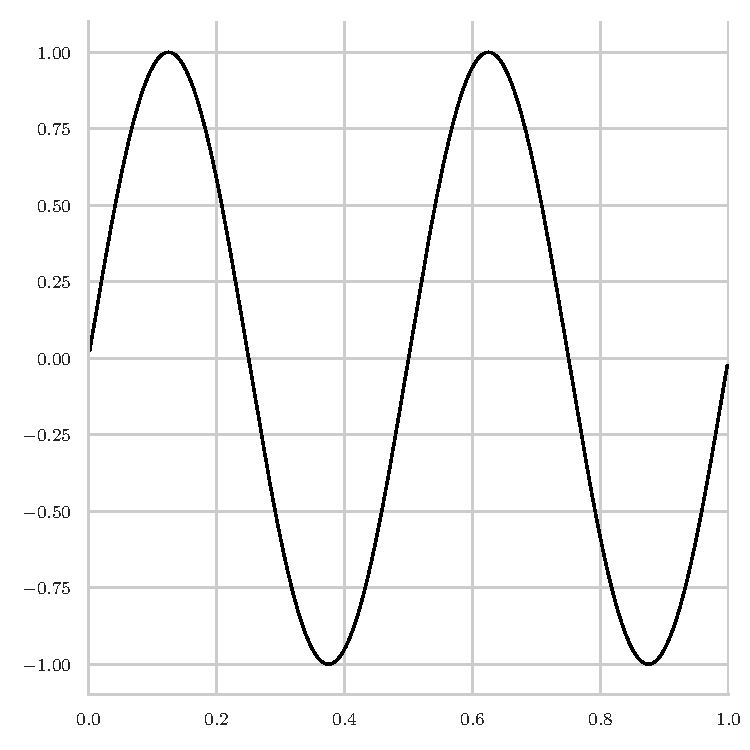
\includegraphics[width=\textwidth]{figures/error_plots//initial_error_jacobi_4pi.pdf}
		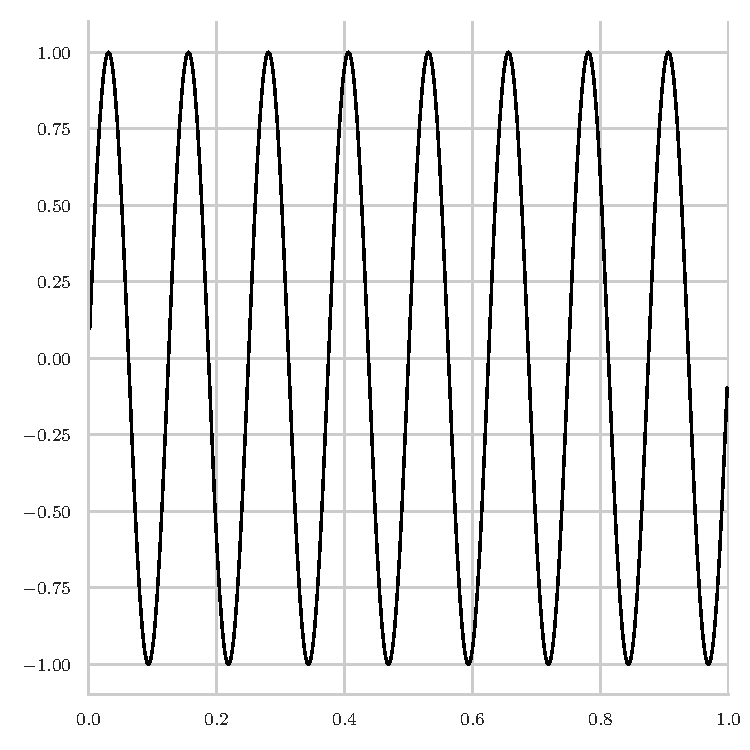
\includegraphics[width=\textwidth]{figures/error_plots//initial_error_jacobi_16pi.pdf}
		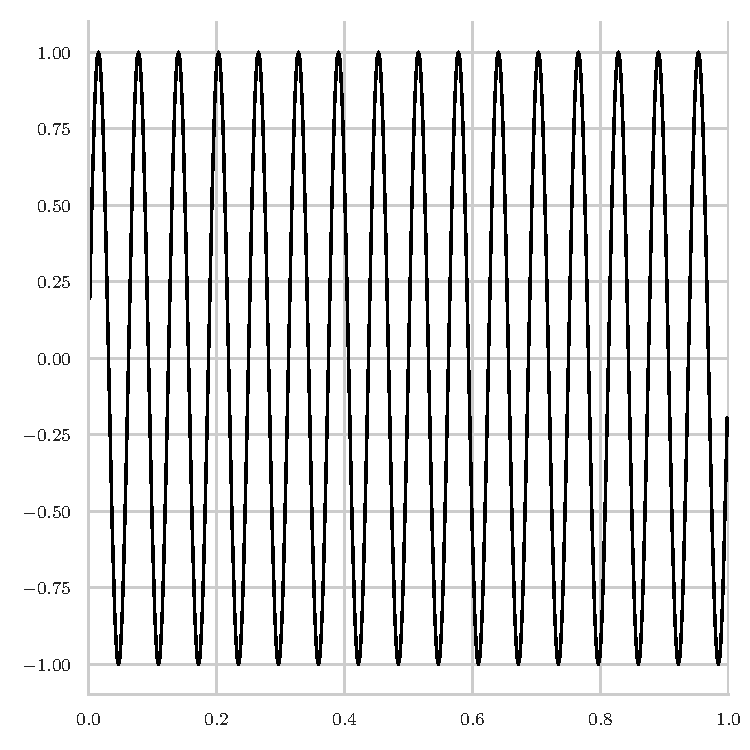
\includegraphics[width=\textwidth]{figures/error_plots//initial_error_jacobi_32pi.pdf}
		\caption{Initial error}
	\end{subfigure}
	\hfill
	\begin{subfigure}[t]{0.32\textwidth}
		\centering
		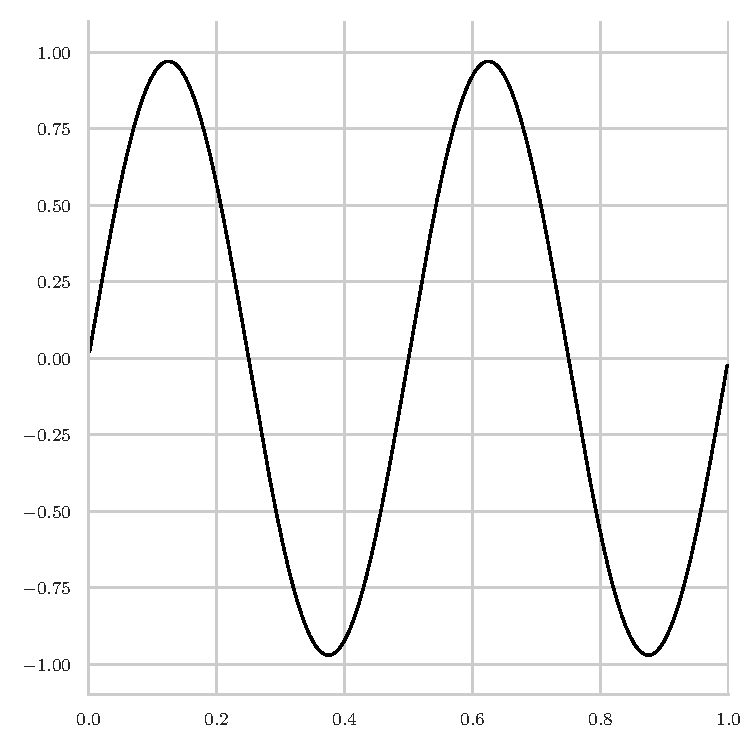
\includegraphics[width=\textwidth]{figures/error_plots//final_error_jacobi_4pi.pdf}
		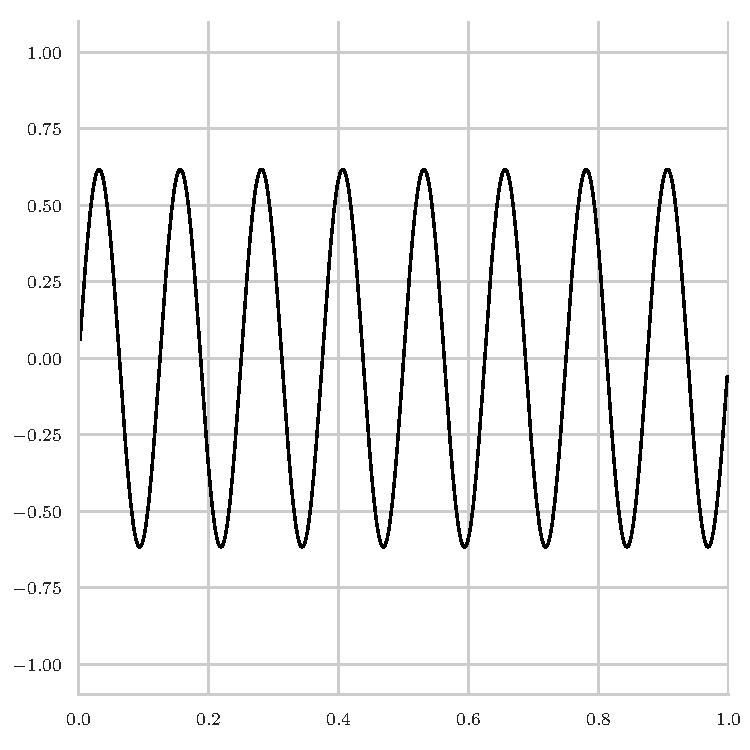
\includegraphics[width=\textwidth]{figures/error_plots//final_error_jacobi_16pi.pdf}
		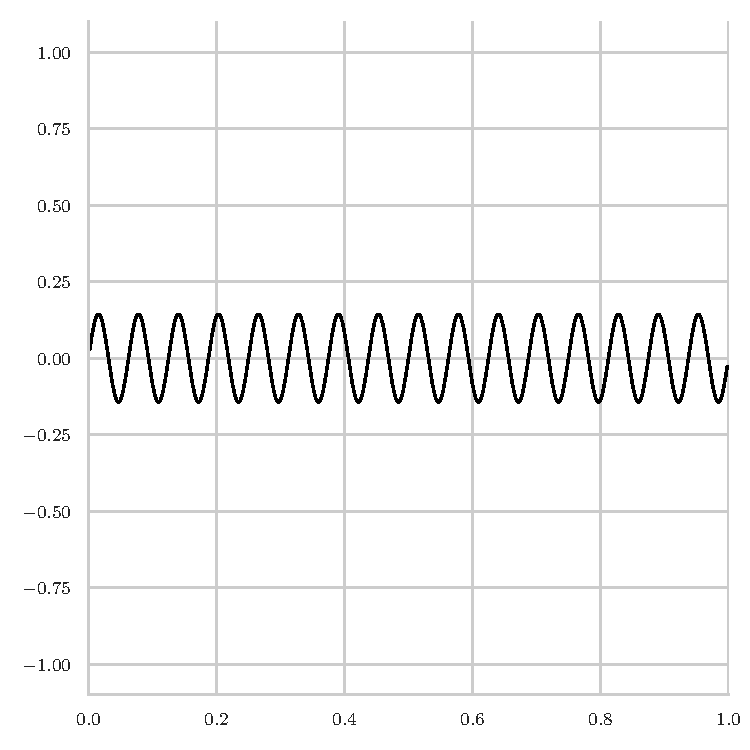
\includegraphics[width=\textwidth]{figures/error_plots//final_error_jacobi_32pi.pdf}
	\caption{Error after applying Jacobi}
	\end{subfigure}
	\hfill
	\begin{subfigure}[t]{0.32\textwidth}
		\centering
		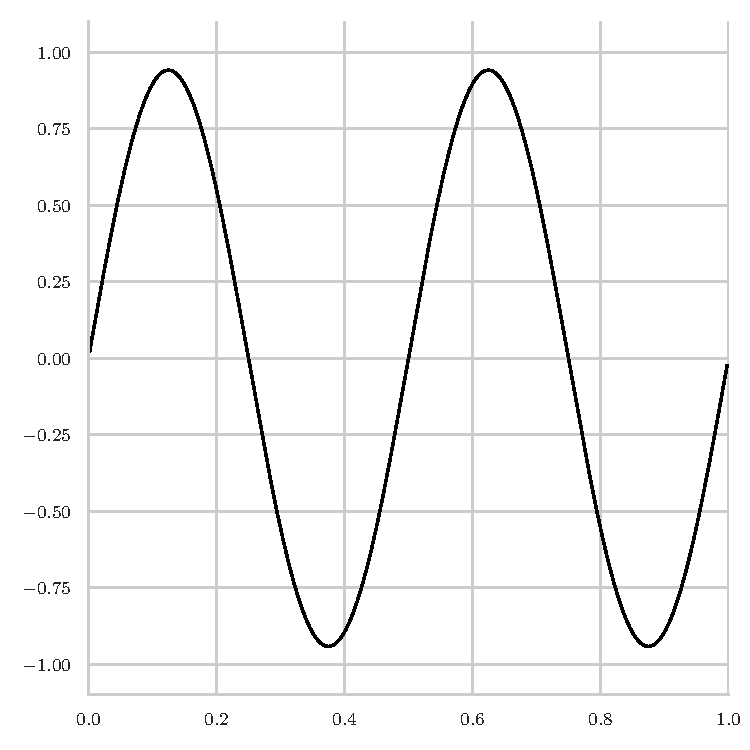
\includegraphics[width=\textwidth]{figures/error_plots//final_error_gauss_seidel_4pi.pdf}
		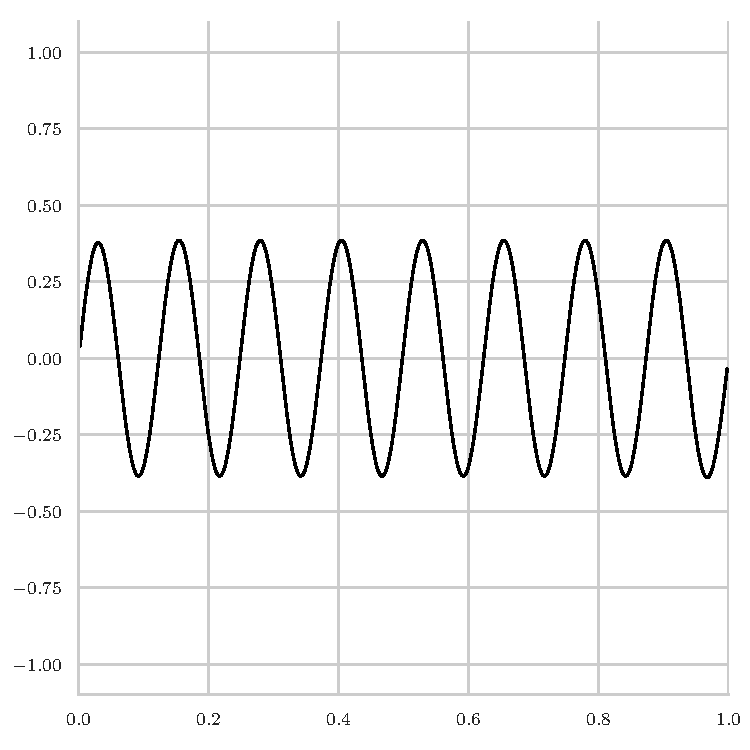
\includegraphics[width=\textwidth]{figures/error_plots//final_error_gauss_seidel_16pi.pdf}
		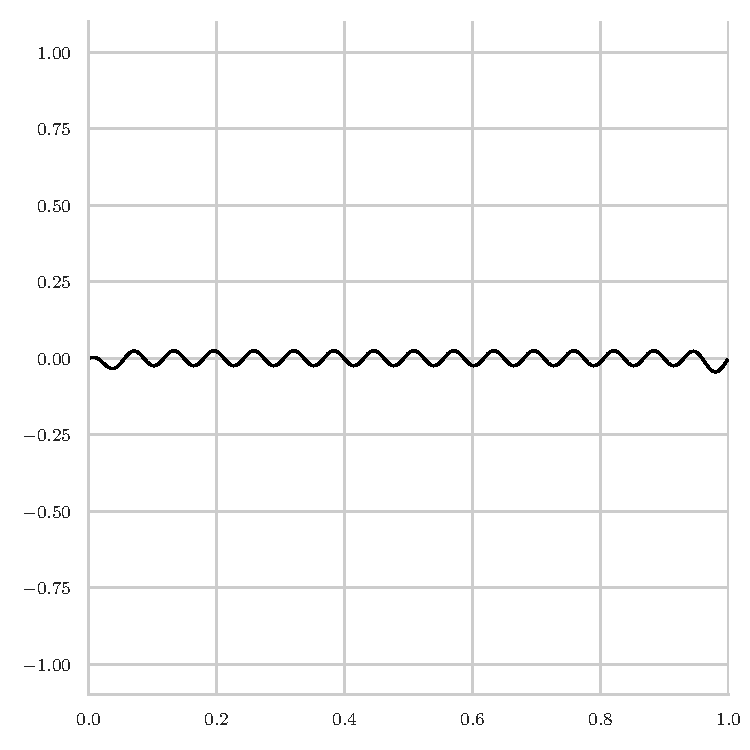
\includegraphics[width=\textwidth]{figures/error_plots//final_error_gauss_seidel_32pi.pdf}
	\caption{Error after applying GS}
	\end{subfigure}
	\caption{Different error components on a one-dimensional grid with step size $h = 2^{-9}$ before and after applying 100 steps of the Jacobi or Gauss-Seidel (GS) method.}
	\label{fig:different-error-components}
\end{figure}
Here, the first column shows the initial error discretized on a grid with step size $h = 2^{-9}$ while the second and third include the remaining error after applying 100 Jacobi and Gauss-Seidel steps, respectively.
Note that the frequency of change increases from top to bottom, whereas the amplitude of the error is always the same.
As can be seen in the second and third column of the first row of Figure~\ref{fig:different-error-components}, the Jacobi and Gauss-Seidel methods do not yield a significant reduction of the low-frequency error components within 100 iterations.
In contrast, in the third row, which shows a highly-oscillating component, the application of 100 steps of the Jacobi method already reduces the initial error to less than one-fifth of its original value.
The same behavior can also be observed for the Gauss-Seidel method, whereby, compared to the Jacobi method, high-frequency error components are reduced even faster.
We can further illustrate the error reduction properties of basic iterative methods by investigating Figure~\ref{fig:combined-error}, which contains a combination of two error components with equal magnitude, one of them with low and the other one with high frequency.
\begin{figure}
	\begin{subfigure}[t]{0.32\textwidth}
	\centering
		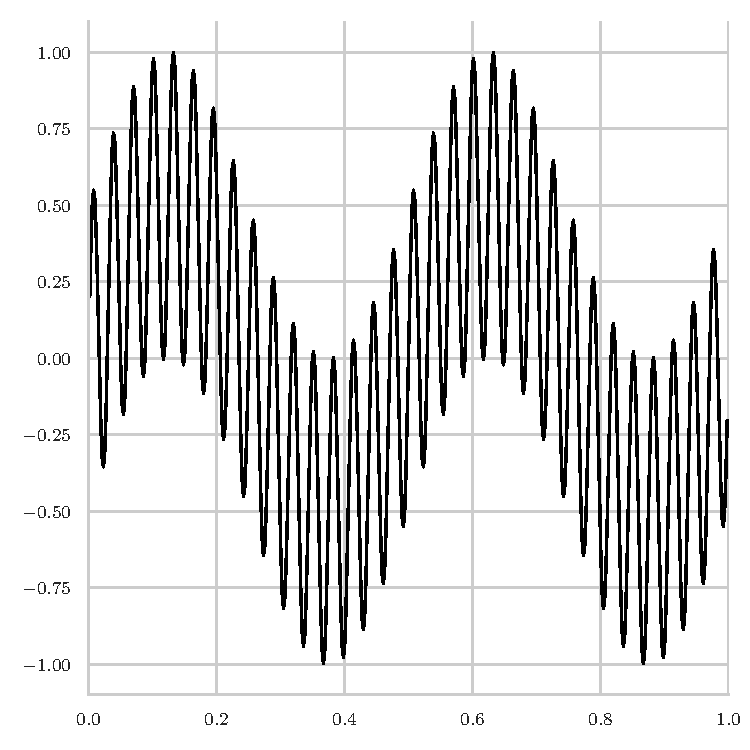
\includegraphics[width=\textwidth]{figures/error_plots//initial_error_jacobi_combined.pdf}
		\caption{Initial error}
\end{subfigure}
\hfill
\begin{subfigure}[t]{0.32\textwidth}
	\centering
		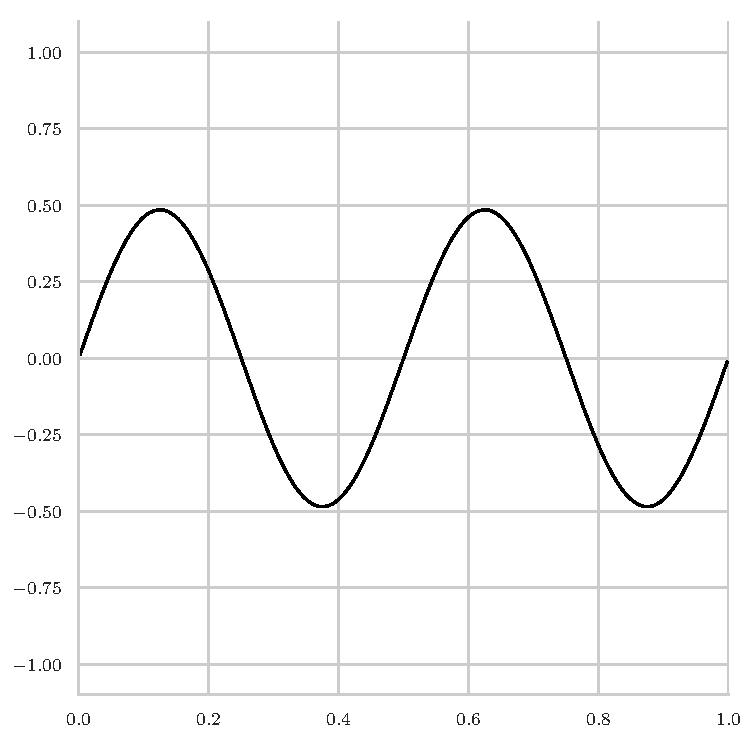
\includegraphics[width=\textwidth]{figures/error_plots//final_error_jacobi_combined.pdf}
		\caption{Error after applying Jacobi}
\end{subfigure}
\begin{subfigure}[t]{0.32\textwidth}
	\centering
	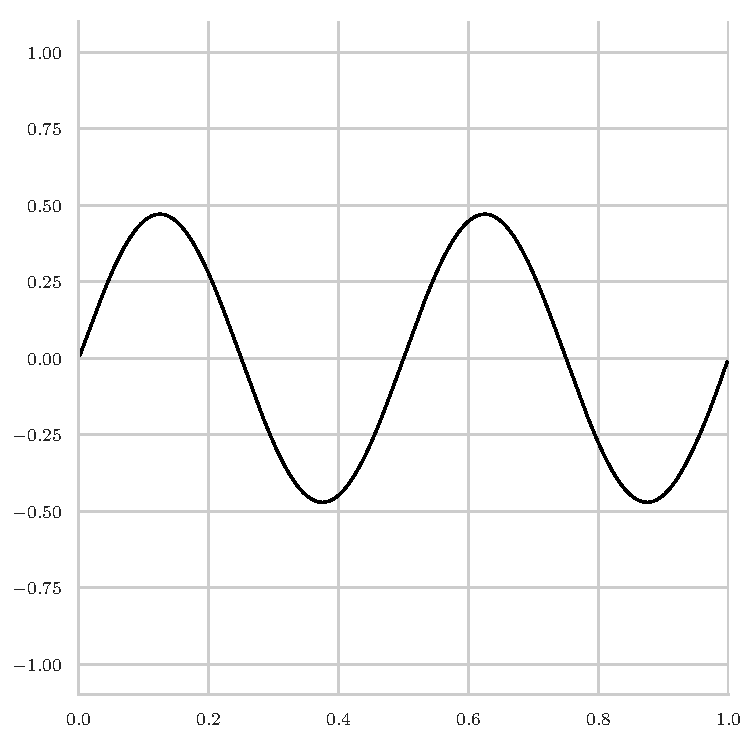
\includegraphics[width=\textwidth]{figures/error_plots//final_error_gauss_seidel_combined.pdf}
	\caption{Error after applying GS}
\end{subfigure}
	\caption{Combination of two error components discretized on a one-dimensional grid with step size $h = 2^{-9}$ before and after applying 100 steps of the Jacobi or Gauss-Seidel (GS) method.}
\label{fig:combined-error}
\end{figure}
Again, the first plot shows the initial error, while the second and third contain the reduced error after 100 iterations of Jacobi and Gauss-Seidel, respectively.
In accordance with our previous observations, the attained improvement achieved with both methods can be almost fully attributed to the reduction of the highly-oscillating component.
Because the remaining error is more smooth than initially, basic iterative methods are often called \emph{smoothers}, and their effectiveness is measured in terms of their capability to reduce the high-frequency components of a given error. 

Now observe what happens if we represent the same low-frequency error component shown in the first row of Figure~\ref{fig:different-error-components} on a grid with larger step size $h = 2^{-6}$ and, thus, a smaller number of grid points.
Because the number of (inner) grid points $n = 1/h - 1$ is inversely proportional to the step size, we call such a grid \emph{coarser}.
The resulting error reduction, again after 100 iterations of each method, is shown in Figure~\ref{fig:low-frequency-error-component-coarse}. 
\begin{figure}
	\begin{subfigure}[t]{0.32\textwidth}
	\centering
	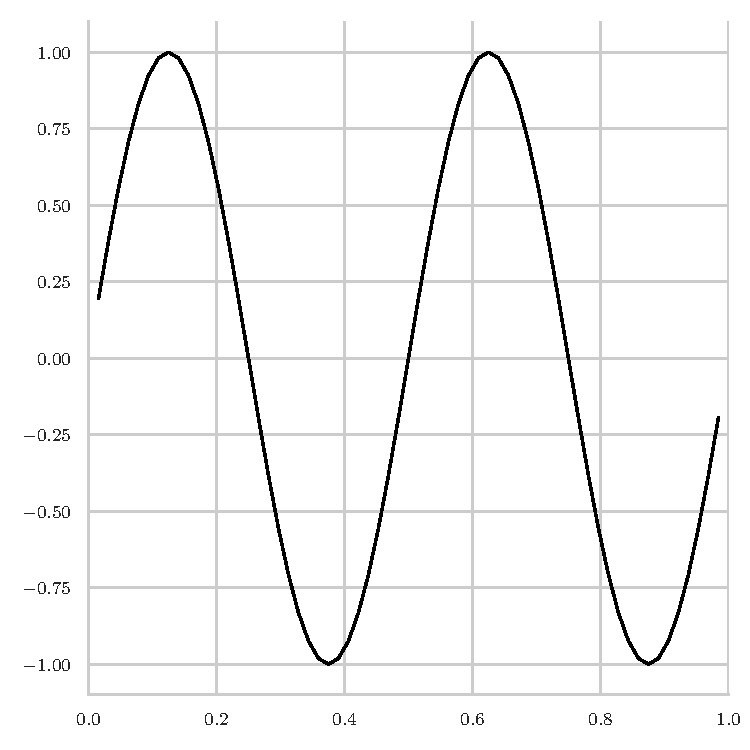
\includegraphics[width=\textwidth]{figures/error_plots//initial_error_jacobi_4pi_coarse.pdf}
	\caption{Initial error}
\end{subfigure}
\hfill
\begin{subfigure}[t]{0.32\textwidth}
	\centering
	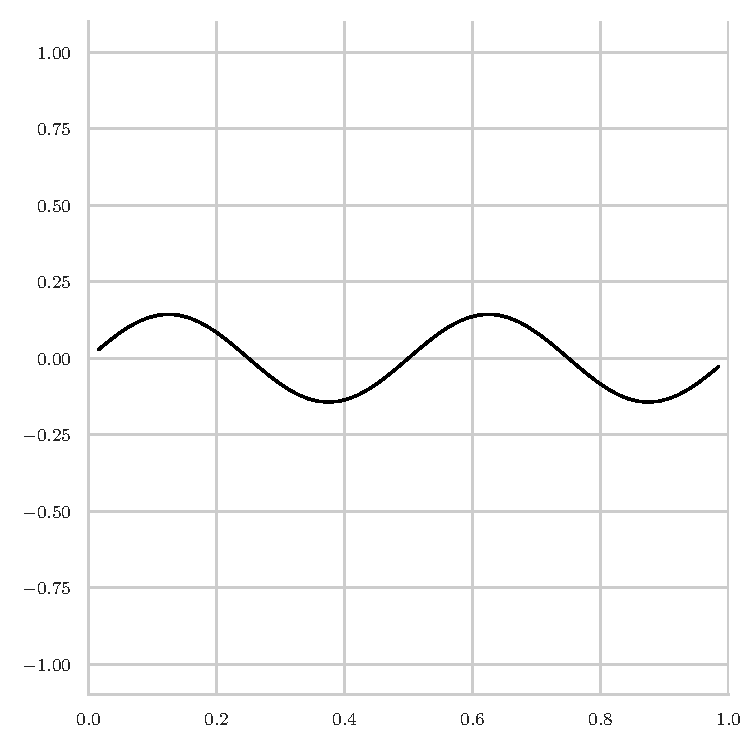
\includegraphics[width=\textwidth]{figures/error_plots//final_error_jacobi_4pi_coarse.pdf}
	\caption{Error after applying Jacobi}
\end{subfigure}
	\hfill
	\begin{subfigure}[t]{0.32\textwidth}
		\centering
		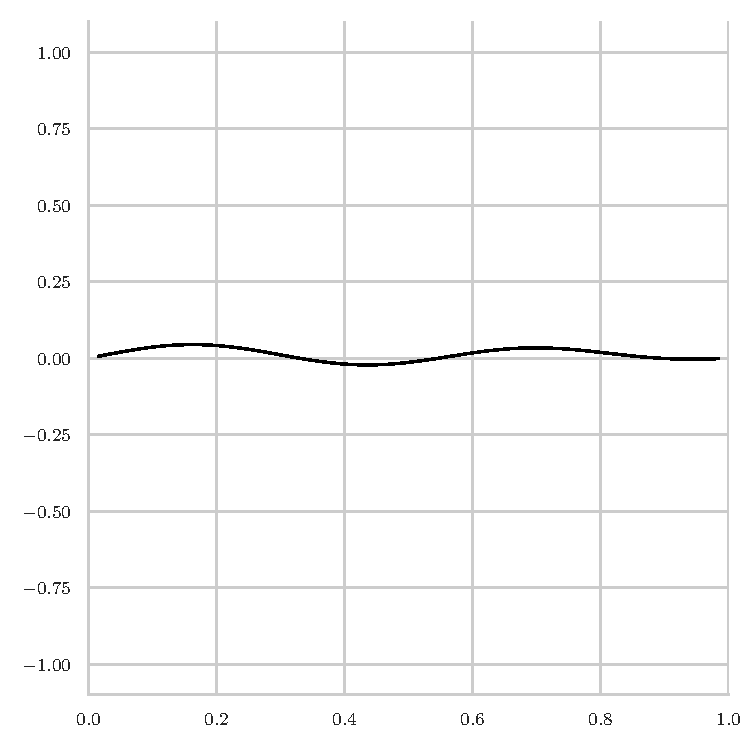
\includegraphics[width=\textwidth]{figures/error_plots//final_error_gauss_seidel_4pi_coarse.pdf}
		\caption{Error after applying GS}
	\end{subfigure}
	\caption{Low-frequency error component discretized on a coarser one-dimensional grid with step size $h = 2^{-6}$ before and after applying 100 steps of the Jacobi or Gauss-Seidel (GS) method.}
	\label{fig:low-frequency-error-component-coarse}
\end{figure}
As it can be seen, the amount of low-frequency error reduction is significantly higher for both methods than on the \emph{finer} grid with a step size of $h = 2^{-9}$.
While smoothers, such as Jacobi and Gauss-Seidel, are only effective in reducing the high-frequency components of a given error, we can overcome this limitation by representing the remaining error on a coarser grid.
Since, on this level, the remaining low-frequency components become more oscillatory, smoothing regains its effectiveness. 
\emph{Multigrid} methods extend this idea by recursively obtaining a coarser representation of the same problem, whose error can then be effectively reduced by employing only a few \emph{smoothing} iterations.
The result is then used to extinguish the remaining error on the next-higher level.
In the following, we introduce the basic components of multigrid methods, i.e., the smoothing, restriction, prolongation, and coarse-grid correction operations.
%Based on this definition, we then develop a formal language for the representation of multigrid solvers.
\subsection{Smoothing}
\label{subsec:smoothing}
One of the central elements of multigrid methods is the utilization of a smoothing procedure for quickly reducing the oscillatory components of a given error.
We have already shown that the Jacobi and Gauss-Seidel method behave in such a way for the considered one-dimensional model problem.
To further improve the smoothing effectiveness of an iterative method, it is often beneficial to introduce an additional relaxation factor $\omega$, which yields the iteration 
\begin{equation}
	\bm{x}^{(k+1)} = \bm{x}^{(k)} + \omega M^{-1}(\bm b - A \bm{x}^{(k)}).
	\label{eq:general-weighted-stationary-iterative-method}
\end{equation}
Again, the weighted Jacobi or Gauss-Seidel method is obtained by replacing the matrix $M$ with the respective term.
\subsubsection{Red-Black Gauss-Seidel}
\label{sec:rb-gs}
While the Gauss-Seidel method often exhibits a superior smoothing property compared to the Jacobi method~\cite{briggs2000multigrid,trottenberg2000multigrid}, each iteration requires solving a lower triangular system of the form
\begin{equation*}
	(D - L) (\bm{x}^{(k+1)} - \bm{x}^{(k)}) = \bm{b} - A \bm{x}^{(k)},
\end{equation*}
with $D - L$ as the lower triangular part of the system matrix $A$.
Since $U = A - (D - L)$, we can rewrite this equation to obtain
\begin{equation}
	(D - L) \bm{x}^{(k+1)} = \bm{b} - U \bm{x}^{(k)},
\end{equation}  
which can then be solved using forward substitution by computing
\begin{equation}
	x_{i}^{(k+1)}={\frac {1}{a_{ii}}}\left(b_{i}-\sum _{j=1}^{i-1}a_{ij}x_{j}^{(k+1)}-\sum _{j=i+1}^{n}a_{ij}x_{j}^{(k)}\right),
	\label{eq:gauss-seidel-element-wise}
\end{equation}
where $x_{i}^{(k)}$ represents the $i$th element of the vector $\bm{x}^{(k)}$.
However, because $x_{i+1}^{(k)}$ depends on $x_{i}^{(k)}$ this computation can only be performed sequentially, which means that the individual components of $\bm{x}^{(k+1)}$ must be computed one after another. 
Modern compute architectures exhibit an ever-increasing degree of parallelism, and hence we must be able to perform all computations in parallel to fully utilize their capabilities.
Now consider the Jacobi method as defined by 
\begin{equation*}
	\bm{x}^{(k+1)} = \bm{x}^{(k)} + D^{-1}(\bm b - A \bm{x}^{(k)}).
\end{equation*}
Similar to the Gauss-Seidel method, we can rewrite this equation to obtain
\begin{equation}
	\bm{x}^{(k+1)} = D^{-1}(\bm b - (A - D)\bm{x}^{(k)}),
\end{equation}
which yields the following element-wise formulation of the Jacobi method:
\begin{equation}
x_{i}^{(k+1)}={\frac {1}{a_{ii}}}\left(b_{i}-\sum _{j\neq i}a_{ij}x_{j}^{(k)}\right).
	\label{eq:jacobi-element-wise}
\end{equation}
In contrast to Equation~\eqref{eq:gauss-seidel-element-wise} the computation of each subsequent element of the vector $\bm{x}^{(k+1)}$ does not depend on any previous one.
Consequently, the computation of each individual element of the new approximate solution $\bm{x}^{(k+1)}$ can be performed completely in parallel.

One possibility to enable a parallel Gauss-Seidel-like computation of the approximate solution $\bm{x}^{(k+1)}$ is to partition the grid points into multiple subsets.
The computation of each subset is then performed in a Jacobi-like fashion using the updated values from other subsets.
A common variant of this approach is the \emph{red-black Gauss-Seidel} (RB-GS) method.
Here, the grid points are assigned to two distinct subsets, where the first represents the red and the second one the black points.
We can define the RB-GS method in the following way:
\begin{equation}
	\begin{split}
		& \bm{x}^{(k+1/2)} = \bm{x}^{(k)} + P_r D^{-1} (\bm{b} - A \bm{x}^{(k)}) \\
		& \bm{x}^{(k+1)} = \bm{x}^{(k+1/2)} + P_b D^{-1} (\bm{b} - A \bm{x}^{(k+1/2)})
	\end{split}
\end{equation}
The entries of the matrices $P_R$ and $P_B$ are then defined as
\begin{equation}
	P_{R,ij} = \begin{cases}
	1 & \text{if} \; i = j \; \text{and} \; i,j \in R \\
	0 & \text{otherwise},  
	\end{cases}
\end{equation}
\begin{equation}
	P_{B,ij} = \begin{cases}
		1 & \text{if} \; i = j \; \text{and} \; i,j \in B \\
		0 & \text{otherwise},
	\end{cases}
\end{equation}
where $R$ and $B$ are the sets of grid indices that correspond to the red and black points, respectively.
For instance, an RB-GS method for the three-point stencil defined in Equation~\eqref{eq:1D-laplace-stencil} can be formulated as
\begin{equation}
\begin{split}
   	& x_{2i}^{(k+1/2)} = \frac {1}{2}\left(h^2 b_{2i} + x_{2i+1}^{(k)} + x_{2i-1}^{(k)}\right) \\
    & x_{2i+1}^{(k+1)} = \frac {1}{2}\left(h^2 b_{2i+1} + x_{2i+2}^{(k+1/2)} + x_{2i}^{(k+1/2)}\right),
\end{split}
\end{equation}
where each grid point with an even index belongs to the red and each one with an odd index to the black points.
Note that the update of each grid point is exclusively based on its neighbors, which have already been updated in the previous step of the method.
By always assigning neighboring points to different partitions, a similar effect can be achieved on any $d$-dimensional grid. 
For instance, a suitable partitioning for the discretized Laplace operator $\Delta_h$ is given by
\begin{equation}
		R = \{ \bm{i} : \bm{i} \in \mathbb{N}^d, \sum_{k=1}^d i_k \; \text{even} \}, \;
		B = \{ \bm{i} : \bm{i} \in \mathbb{N}^d, \sum_{k=1}^d i_k \; \text{odd} \}.
\end{equation}
In many cases, the resulting method has better smoothing properties than the Jacobi method without sacrificing much of its parallelism, as the computations on each partition can be performed concurrently~\cite{trottenberg2000multigrid}.
\subsubsection{Block Smoothing}
\label{subsec:block-smoothing}
So far, we have only discussed smoothers that operate in a pointwise manner.
For instance, in the Jacobi method Equation~\eqref{eq:jacobi-element-wise} is computed for each individual grid point.
The idea of block smoothing is to reorder the original system in such a way, that the same operations can be defined on small subsets of grid points, which are chosen in the form of rectangular blocks of a particular size.
As a consequence, each scalar operation in the original pointwise method is replaced by a matrix or vector operation, whose dimensionality corresponds to the chosen block size.

For example, we can rearrange our original system of the form of Equation~\eqref{eq:general-system-of-linear-equations} in the following way:
\begin{equation}
\underbrace{
\begin{pmatrix}A_{11}&A_{12}&\cdots &A_{1m}\\A_{21}&A_{22}&\cdots &A_{2m}\\\vdots &\vdots &\ddots &\vdots \\A_{m1}&A_{m2}&\cdots &A_{mm}\end{pmatrix}}_{A}
 = 
\underbrace{
\begin{pmatrix}
\bm{x}_1 \\ \bm{x}_2 \\ \vdots \\ \bm{x_m} 
\end{pmatrix}}_{\bm{x}} =
\underbrace{
\begin{pmatrix}
	\bm{b}_1 \\ \bm{b}_2 \\ \vdots \\ \bm{b_m} 
\end{pmatrix}}_{\bm{b}}
\end{equation}
where $m = n / n_b$, if $n_b$ is the size of each block.
A block Jacobi method can then be defined as
\begin{equation}
	\bm{x}_{i}^{(k+1)}=A_{ii}^{-1}\left(\bm{b}_{i}-\sum _{j\neq i}A_{ij}\bm{x}_{j}^{(k)}\right),
	\label{eq:jacobi-block-wise}
\end{equation}
For example, choosing a block size of two for the one-dimensional Laplace equation yields
\begin{equation}
	\begin{pmatrix}
		2 & -1 \\
		-1 & 2
	\end{pmatrix}
	\begin{pmatrix}
		x_{j}^{(k+1)} \\ x_{j+1}^{(k+1)} 
	\end{pmatrix}
= 	-  \begin{pmatrix}
	0 & 0 \\
	-1 & 0
\end{pmatrix} 	
\begin{pmatrix}
x_{j+2}^{(k)} \\ x_{j+3}^{(k)}
\end{pmatrix} -
\begin{pmatrix}
	0 & -1 \\
	0 & 0
\end{pmatrix} 	
\begin{pmatrix}
	x_{j-2}^{(k)} \\ x_{j-1}^{(k)} 
\end{pmatrix},
\end{equation}
where $j = n_b (i - 1) + 1$.
This method can be defined in a similar way using our previously introduced stencil notation
\begin{equation}
\begin{split}
	& \begin{pmatrix}
		\left[0 \quad 2 \quad -1 \right]_{h} \cdot x_{j}^{(k+1)} \\ \left[ -1 \quad 2 \quad 0 \right]_{h} \cdot x_{j+1}^{(k+1)} 
	\end{pmatrix}
	= \\ - & 
	\begin{pmatrix}
		\left[ 0 \right]_{h} \cdot x_{j+2}^{(k)} \\ \left[-1 \quad 0 \quad 0 \right]_{h} \cdot x_{j + 3}^{(k)}
	\end{pmatrix} -
	\begin{pmatrix}
		\left[0 \quad 0 \quad -1 \right]_{h} \cdot x_{j-2}^{(k)} \\ \left[ 0 \right]_{h} \cdot x_{j-1}^{(k)} 
	\end{pmatrix}.
\end{split}
\end{equation}
In both cases, we obtain a system of two linear equations
\begin{equation}
	\begin{pmatrix}
		2 x_{j}^{(k+1)} - x_{j+1}^{(k+1)} \\ 2 x_{j+1}^{(k+1)} - x_{j}^{(k+1)} 
	\end{pmatrix}
	=
	\begin{pmatrix}
		x_{j - 1}^{(k)} \\ x_{j + 2}^{(k)}
	\end{pmatrix}.
\end{equation}
which must be solved for each block, for instance, using a direct solver such as Gaussian elimination.
As in the pointwise Jacobi method, each block can be solved independently and, therefore, operations on different blocks can be performed in parallel. 
Considering the fact that a direct solver in general require $\mathcal{O}(n_b^3)$ operations to solve each block, the overall computational cost of applying a block smoother can be estimated with $\mathcal{O}(n_b^3 \frac{n}{n_b}) = \mathcal{O}(n_b^2 n)$.
Note that choosing $n_b = n$ means that we treat the whole matrix $A$ as a single block and, therefore, solve the original system using Gaussian elimination.
In contrast, the choice of $n_b = 1$ corresponds to the pointwise Jacobi method, which, for a constant stencil, can be computed with a constant number of operations per grid point.
While we here only provide a brief introduction to block smoothers, it must be mentioned that it is also possible to define block variants for other smoothers, such as the Gauss-Seidel and red-black Gauss-Seidel method.
Finally, alternatively, it is also possible to define overlapping block smoothers, which means that multiple blocks contain the same grid point as an unknown~\cite{trottenberg2000multigrid}.

\subsection{The Coarse-Grid Correction Scheme}
The core idea behind multigrid methods is to reduce the oscillatory components of an error by obtaining an approximation of the same problem on a coarser grid.
As we have illustrated in Figure~\ref{fig:low-frequency-error-component-coarse} these components can then be reduced quickly using the same smoothing techniques employed on the fine grid.
Before we can define this approach algorithmically, note that our original system
\begin{equation}
	A_h \bm{x}_h = \bm{b}_h
\end{equation}
is equivalent to the error equation
\begin{equation}
	A_h \left(\bm{x}_h - \bm {x}^{(0)}_h\right) = \bm{b}_h - A_h \bm{x}^{(0)}_h
\end{equation}
with the arbitrary-chosen initial guess $\bm{x}^{(0)}_h$.
The subscripts $A_h$ and $\bm{x}_h$ indicate a discretization with step size $\bm{h}$.
Therefore, each entry of the vector $\bm{x}_h$ represents a grid function value $u_h(\bm{i} \cdot \bm{h})$ at the respective position within the grid.
We can further introduce the error $\bm{e}_h = \bm{x}_h - \bm {x}^{(0)}_h$ to obtain the equation
\begin{equation}
	A \bm{e} = \bm{b} - A \bm{x}^{(0)}.
	\label{eq:linear-system-error-equation}
\end{equation}
Based on the solution $\bm{e}_h$ of this system, which depends on the initial solution $\bm{x}^{(0)}_h$, we can, again, obtain the solution of the original system by computing
\begin{equation}
	\bm{x}_h = \bm{x}^{(0)}_h + \bm{e}_h.
\end{equation}
Now, assume there exists both a prolongation and restriction operator, $I_h^{2h}$ and $I_{2h}^h$, that enables us to compute an approximation for a given variable $\bm{x}_h$ on a coarser and finer grid, respectively, such that
\begin{equation}
	\bm{x}_{2h} \approx I_h^{2h} \bm{x}_{h}, \;
	\bm{x}_{h} \approx I_{2h}^{h} \bm{x}_{2h}. 
\end{equation}
In general, this approximation can obviously never be exact.
However, we have already observed that if a certain error exclusively consists of smooth components, we can approximate them on a coarser grid without a significant loss of accuracy.
This is illustrated in Figure~\ref{fig:error-on-multiple-levels}, which shows the discretization of two error components with different frequencies on one-dimensional uniform grids with decreasing step size.
Here, the first error component, which possesses a higher frequency, can not be accurately represented on the coarsest grid with step size $h = 2^{-5}$.
In contrast, the course of the second error component, which is relatively smooth, is still clearly visible on the same grid. 
\begin{figure}
	\begin{subfigure}[b]{0.32\textwidth}
		\centering
		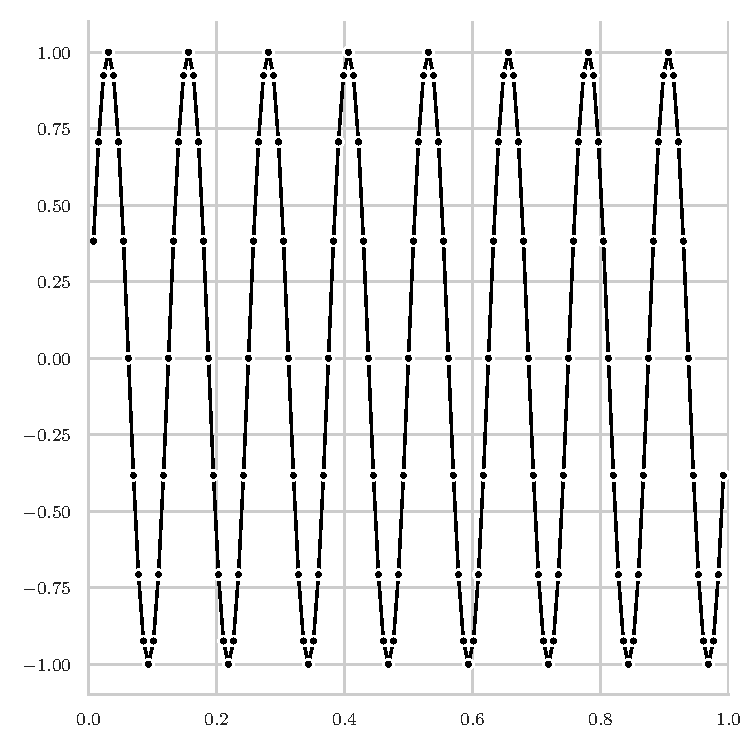
\includegraphics[width=\textwidth]{figures/error_plots//initial_error_16pi_level7.pdf}
	\end{subfigure}
	\hfill
	\begin{subfigure}[b]{0.32\textwidth}
		\centering
		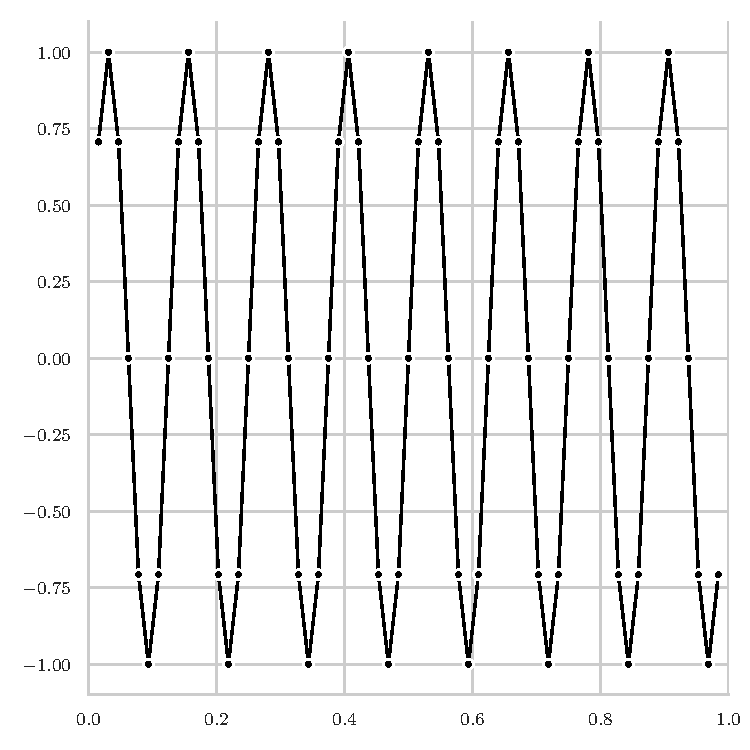
\includegraphics[width=\textwidth]{figures/error_plots//initial_error_16pi_level6.pdf}
	\end{subfigure}
	\hfill
	\begin{subfigure}[b]{0.32\textwidth}
		\centering
		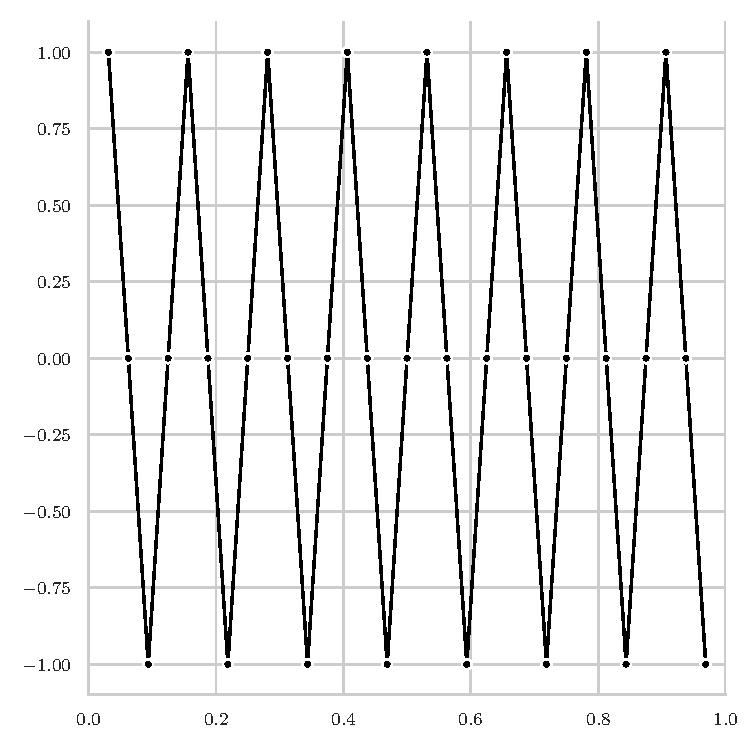
\includegraphics[width=\textwidth]{figures/error_plots//initial_error_16pi_level5.pdf}
	\end{subfigure}
		\begin{subfigure}[b]{0.32\textwidth}
		\centering
		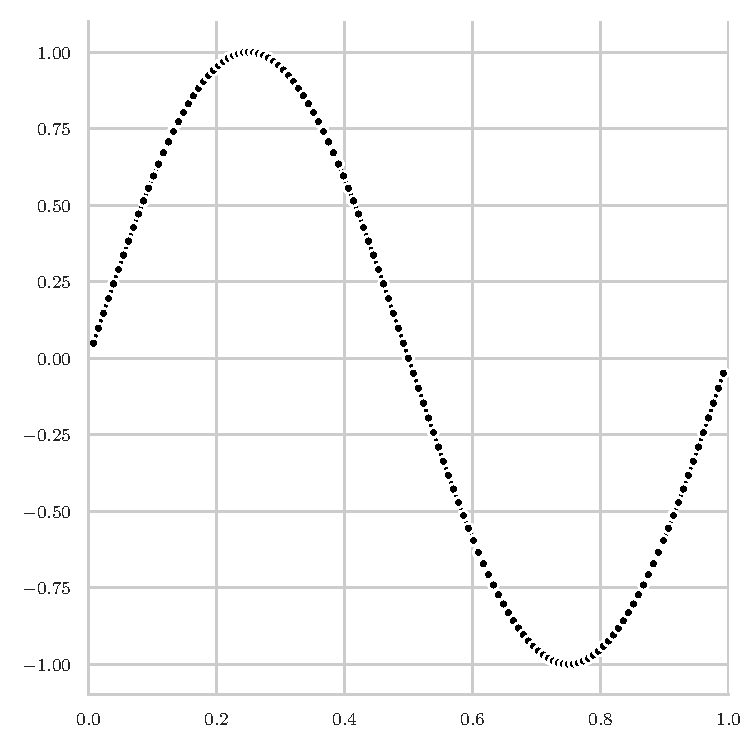
\includegraphics[width=\textwidth]{figures/error_plots//initial_error_2pi_level7.pdf}
		\caption{$h = 2^{-7}$}
	\end{subfigure}
	\hfill
	\begin{subfigure}[b]{0.32\textwidth}
		\centering
		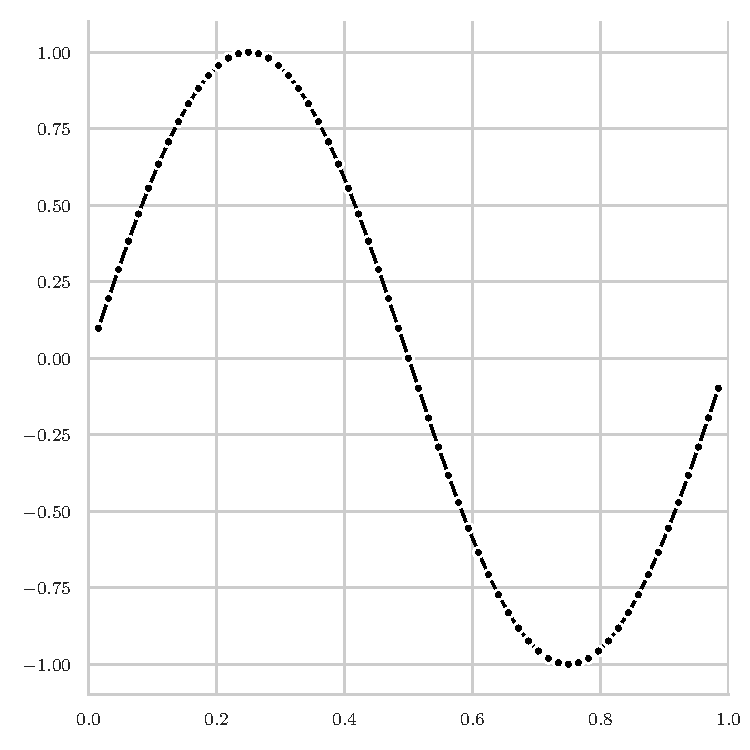
\includegraphics[width=\textwidth]{figures/error_plots//initial_error_2pi_level6.pdf}
		\caption{$h = 2^{-6}$}
	\end{subfigure}
	\hfill
	\begin{subfigure}[b]{0.32\textwidth}
		\centering
		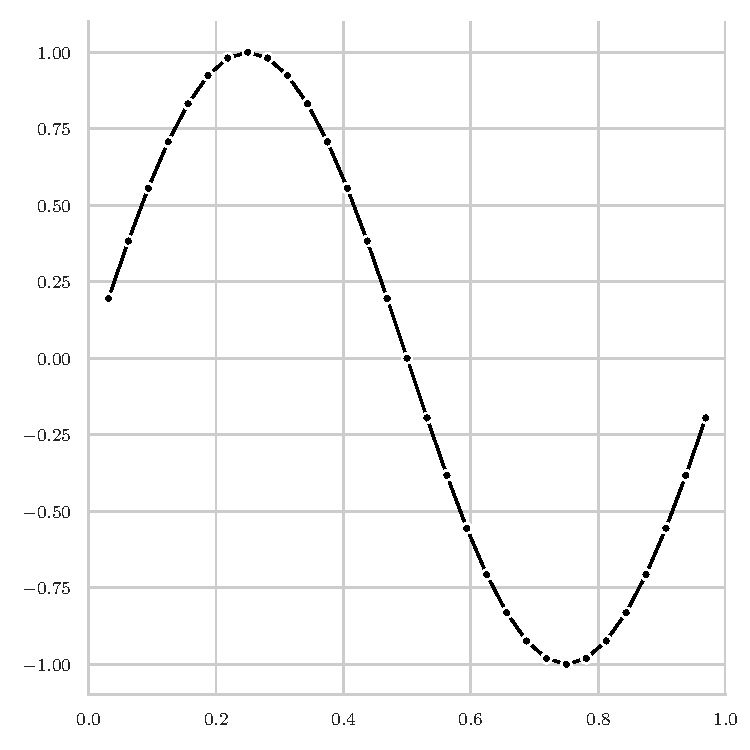
\includegraphics[width=\textwidth]{figures/error_plots//initial_error_2pi_level5.pdf}
		\caption{$h = 2^{-5}$}
	\end{subfigure}
	\caption{Oscillatory and smooth error components discretized on a hierarchy of grids with decreasing step size.}
	\label{fig:error-on-multiple-levels}
\end{figure}
Assuming that the error $\bm{e}_{2h}$ on the coarse grid consists exclusively of smooth components and, hence, $\bm{e}_{h} \approx I_{2h}^{h} \bm{e}_{2h}$, we can define the coarse grid correction 
\begin{equation}
	\bm{x}^{k+1}_h = \bm{x}^{k}_h + I_{2h}^h \bm{e}_{2h}.
\end{equation} 
Now the question remains to be answered how we can compute an approximation for the error $\bm{e}_{2h}$ on the coarse grid.
As we have pointed out above, Equation~\eqref{eq:linear-system-error-equation} is equivalent to the original system.
We can, therefore, can apply our previously defined inter-grid transfer operators to define the error equation on a coarser grid with step size $2\bm{h}$
\begin{equation}
	\underbrace{I_{h}^{2h} A_h I_{2h}^h}_{A_{2h}} \bm{e}_{2h} = I_{h}^{2h} \left(\bm{b}_h - A_h \bm{x}^{(0)}_h\right).
	\label{eq:coarse-grid-error-equation}
\end{equation}
Note that we have again made use of the fact that in case $\bm{e}_{2h}$ is smooth, $\bm{e}_{h} \approx I_{2h}^{h} \bm{e}_{2h}$ is a reasonably accurate approximation.
Note that in Equation~\eqref{eq:coarse-grid-error-equation} the coarse operator $A_{2h}$ is directly obtained from the original operator $A_{2h}$, which is called \emph{Galerkin coarsening}.
However, in cases where the operator $A_h$ can be directly discretized on a coarser grid with step size $2\bm{h}$, it is often also possible to use the resulting operator $A_{2h}$ instead.
By bringing all these components together, we can formulate the two-level-method shown in Algorithm~\ref{alg:two-grid-method}.
\begin{algorithm}
	\caption{Two-Grid Method}
	\label{alg:two-grid-method}
	\begin{algorithmic}
		\State{Relax on $A_h \bm{x}_h = \bm{b}_h$ to obtain an approximation $\tilde{\bm{x}}_h$}
		\State{Compute the residual $\bm{r}_h = \bm{b}_h - A_h \tilde{\bm {x}}_h$}
		\State{\hskip1em Obtain $A_{2h}$ through Galerkin coarsening or rediscretization}
		\State{\hskip1em Restrict the residual $\bm{b}_{2h} = I_h^{2h} \bm{r}_h$}
		\State{\hskip1em Solve $A_{2h} \bm{x}_{2h} = \bm{b}_{2h}$ for $\bm{x}_{2h}$}
		\State{Perform the correction $\tilde{\bm{x}}_h = \tilde{\bm{x}}_h + I_{2h}^h \bm{x}_{2h}$}
		\State{Relax again $A_h \bm{x}_h = \bm{b}_h$ with an initial guess of $\tilde{\bm{x}}_h$}
	\end{algorithmic}
\end{algorithm}
Note that while on the coarse grid we are actually solving the error equation, it has been redefined as $A_{2h} \bm{x}_{2h} = \bm{b}_{2h}$.
Based on this notation, we could similarly define a two-level method starting from a grid with step size $2\bm{h}$.
However, to put this approach into practice, we need to choose an initial guess for the error equation on this level.
For this purpose, note that one step of smoothing applied to Equation~\eqref{eq:coarse-grid-error-equation} with an initial guess of zero corresponds to
\begin{equation}
	\bm{e}_{2h}^{(1)} = M_{2h}^{-1} I_{h}^{2h} \left(\bm{b}_h - A_h \bm{x}^{(0)}_h\right).
	\label{eq:initial-coarse-grid-relaxation}
\end{equation}
Since the error $\bm{e}_{2h}^{(k+1)}$ in step $k+1$ is defined as
\begin{equation*}
	\bm{e}_{2h}^{(k+1)} = \bm{x}_{2h}^{(k+1)} - \bm{x}_{2h}^{(k)},
\end{equation*}
and assuming that $\bm{x}_{h}^{(0)}$ is smooth, we can choose $\bm{x}_{2h}^{(0)} = I_{2h}^{h} \bm{x}_{h}^{(0)}$ and, hence, obtain the iteration
\begin{equation}
	\bm{x}_{2h}^{(1)} = I_{h}^{2h} \bm{x}_{h}^{(0)} + M_{2h}^{-1} ( I_{h}^{2h} \bm{b}_h - \underbrace{I_{h}^{2h} A_h I_{2h}^{h}}_{A_{2h}} I_{h}^{2h} \bm{x}_{h}^{(0)} ).
\end{equation}
Performing one smoothing step with an initial guess of zero on the coarse-grid error equation, therefore, corresponds to one smoothing step applied to the equation
\begin{equation}
	I_{h}^{2h} A_h I_{2h}^h \bm{x}_{2h} = I_{h}^{2h} \bm{b}_h,
\end{equation}
with an initial guess of $\bm{x}_{2h}^{(0)} = I_{h}^{2h} \bm{x}_{h}^{(0)}$.
Because smoothing aims to remove the remaining oscillatory components of the error that have been transferred from the fine grid, applying it in the form of Equation~\eqref{eq:initial-coarse-grid-relaxation} precisely serves this purpose.

\subsection{Restriction and Prolongation}
\label{subsec:restriction-and-prolongation}
%TODO fix stencil notation in this section
Before we can define an actual multigrid method, which recursively applies the techniques introduced here to a hierarchy of discretizations consisting of more than two levels, we need to define suitable inter-grid operators, $I_{2h}^{h}$ and $I_{h}^{2h}$.
Here, the restriction operator $I_{2h}^{h}$ should yield an accurate approximation of the current residual on a coarser grid, while the goal of the prolongation operator $I_{h}^{2h}$ is to transfer the computed solution of the error equation back to a finer grid.
In both cases, we are, first and foremost, interested in preserving the low-frequency components, as the remaining ones will be quickly reduced by smoothing.
In general, the implementation of these operators depends on the chosen method of discretization. 
Since, as mentioned in Section~\ref{sec:discretization}, this work focuses on the discretizations of PDEs on regular grids, we do not consider inter-grid operators defined on other grid types, such as unstructured grids.
For a detailed treatment of these cases, the reader is referred to~\cite{trottenberg2000multigrid,ruge1987algebraic,stuben2001introduction}.
As a first step towards defining a suitable restriction operator, note that on a regular grid, the set of coarse-grid points is always contained in the set of fine-grid points.
Therefore, the easiest way to define such an operator is to simply carry over the values present at the respective points of the fine grid over to the coarse grid, which leads to the so-called \emph{injection} restriction operator.
While this approach can lead to a functioning multigrid method in case the residual is sufficiently smooth, it neglects the information contained within all fine grid points that do not coincide with a coarse grid point.
In most cases, it is beneficial to incorporate this information into the coarse grid by computing a weighted average over all neighboring fine grid points.
This idea leads to the so-called \emph{full-weighting} and \emph{half-weighting} restriction operators.
Using our previously defined stencil notation, the one-dimensional full-weighting restriction operator is given by
\begin{equation}
	I_{h}^{2 h} = \frac{1}{4}\{((-1), 1), ((0), 2), ((1), 1)\}_{h_x}^{2h}
\end{equation} 
or equivalently using the matrix notation
\begin{equation}
	I_{h}^{2h} =  \frac{1}{4} \begin{bmatrix}
			1 & 2 & 1
		\end{bmatrix}_{h_x}^{2h}.
	\label{eq:full-weighting-restriction}
\end{equation} 
If we treat Equation~\eqref{eq:full-weighting-restriction} as a row vector, we can define the two- and three-dimensional full-weighting restriction operator as a tensor product with the corresponding column vector, such that
\begin{equation}
	I^{2h_x, 2h_y}_{h_x, h_y} = \frac{1}{4} \begin{bmatrix}
		1 \\ 2 \\ 1
	\end{bmatrix}_{h_y}^{2h_y} \otimes \frac{1}{4} \begin{bmatrix}
		1 & 2 & 1
	\end{bmatrix}_{h_x}^{2h_x} =
\frac{1}{16} 
\begin{bmatrix}
	1 & 2 & 1 \\
	2 & 4 & 2 \\
	1 & 2 & 1
\end{bmatrix}^{2h_x, 2h_y}_{h_x, h_y},
\end{equation} 
\begin{equation}
\begin{split}
	& I^{2h_x, 2h_y, 2h_z}_{h_x, h_y, h_z} = \frac{1}{4} \begin{bmatrix}
		1 & 2 & 1
	\end{bmatrix}_{h_z}^{2h_z} \otimes 
	\frac{1}{16} 
	\begin{bmatrix}
		1 & 2 & 1 \\
		2 & 4 & 2 \\
		1 & 2 & 1
	\end{bmatrix}^{2h_x, 2h_y}_{h_x, h_y} \\
& = \frac{1}{64} \begin{bmatrix}
\begin{bmatrix}
	1 & 2 & 1 \\
	2 & 4 & 2 \\
	1 & 2 & 1
\end{bmatrix} &	\begin{bmatrix}
2 & 4 & 2 \\
4 & 8 & 4 \\
2 & 4 & 2
\end{bmatrix} &
\begin{bmatrix}
	1 & 2 & 1 \\
	2 & 4 & 2 \\
	1 & 2 & 1
\end{bmatrix}
\end{bmatrix}^{2h_x, 2h_y, 2h_z}_{h_x, h_y, h_z}.
\end{split}
\end{equation}
A second restriction operator based on the idea of averaging neighboring fine grid points is the half-weighting restriction operator, whose two- and three-dimensional versions can be defined as
\begin{equation}
	I^{2h_x,2h_y}_{h_x, h_y} = \frac{1}{8}
	\begin{bmatrix}
		0 & 1 & 0 \\
		1 & 4 & 1 \\
		0 & 1 & 0
	\end{bmatrix}^{2h_x}_{h_x},
\end{equation} 
\begin{equation}
\begin{split}
	& I^{2h_x, 2h_y, 2h_z}_{h_x, h_y, h_z} = 
\frac{1}{4} \begin{bmatrix}
	1 & 2 & 1
\end{bmatrix}_{h_z}^{2h_z}
\otimes 
\frac{1}{8}
	\begin{bmatrix}
	0 & 1 & 0 \\
	1 & 4 & 1 \\
	0 & 1 & 0 
\end{bmatrix}^{2h_x,2h_y}_{h_x, h_y} \\
& =
\frac{1}{32} \begin{bmatrix}
	\begin{bmatrix}
		& 1 &  \\
		1 & 4 & 1 \\
		& 1 & 
	\end{bmatrix}
 &		\begin{bmatrix}
 	& 2 &  \\
 	2 & 6 & 2 \\
 	& 2 & 
 \end{bmatrix} &
	\begin{bmatrix}
	& 1 &  \\
	1 & 4 & 1 \\
	& 1 & 
\end{bmatrix}
\end{bmatrix}^{2h_x, 2h_y, 2h_z}_{h_x, h_y, h_z}
\end{split}
\end{equation} 
Note that in contrast to our original definition of the stencil application in Equation~\eqref{eq:stencil-application}, which applies the stencil to each point on the current grid, the restriction stencils presented here only have to be applied to each point on the fine grid that coincides with a coarse-grid point.
We can therefore replace it with the following slightly adapted definition of stencil application
\begin{equation}
	\begin{split}
		& I_{h}^{2h} \cdot u_h(\bm{x}) = \sum_{k=1}^m b_k u_h({\bm x + \bm{a}_k} \circ \bm{h}) \quad 
		\text{with} \; \bm{x} \in G_{2h}, m \in \mathbb{N} \\ & (\bm{a}_k, b_k) \in I_{h}^{2h} \; \forall \, k \in \{ 1, 2, \dots, m \}
	\end{split}
	\label{eq:stencil-restriction-application}
\end{equation}
where $u_h(\bm{x})$ with $\bm{x} \in G_{2h}$ represents an arbitrary point on the fine grid for which there exists a unique coarse-grid point defined at the same spatial position within the computational domain.
Note that this is an immediate consequence of the fact that we have defined the set of coarse-grid points as a subset of the fine-grid points.

On the other hand, for prolongation, our goal is to define an operator that transfers an approximation of the error computed on a certain discretization level to a grid of higher resolution.
We, therefore, must be able to restore a higher number of grid points based on the given values on the coarse grid, which can be regarded as a distribution process.
The application of this operator to a given coarse-grid point $u_{2h}(\bm{x})$ with $\bm{x} \in G_{2h} \supset G_h$ can be defined as
\begin{equation}
	I_{h}^{2h} \cdot u_{2h}(\bm{x}) \rightarrow
	\begin{cases}
		& \forall \, (\bm{a}_k, b_k) \in I_{2h}^{h} \; \text{with} \; k \in \{ 1, 2, \dots, m \} \; \wedge \; \bm{x} \in G_{2h} : \\
		& u_{h}(\bm{x} + \bm{a}_k \circ \bm{h}) = u_{h}(\bm{x} + \bm{a}_k \circ \bm{h}) + b_k u_{2h}(\bm{x}) 
	\end{cases},
	\label{eq:stencil-prolongation application}
\end{equation}
whereby we assume that initially $\forall u_h(\bm{x}) \; \text{with} \; \bm{x} \in \mathcal G_h : u_h(\bm{x}) = 0$.
A common choice for one-dimensional prolongation is the linear interpolation operator~\cite{trottenberg2000multigrid}, which can be defined as
\begin{equation}
	I_{h_x}^{2h} =  \frac{1}{2} \begin{bmatrix}
		1 & 2 & 1
	\end{bmatrix}_{h}^{2h}.
	\label{eq:linear-interpolation}
\end{equation}
Similar to full-weighting restriction, we can derive two- and three-dimensional versions of this operator as tensor products of the form
\begin{equation}
	I_{h_x, h_y}^{2h_x, 2h_y} = \frac{1}{2} \begin{bmatrix}
		1 \\ 2 \\ 1
	\end{bmatrix}_{h_y}^{2h_y} \otimes \frac{1}{2} \begin{bmatrix}
		1 & 2 & 1
	\end{bmatrix}_{h_x}^{2h_x} =
	\frac{1}{4} 
	\begin{bmatrix}
		1 & 2 & 1 \\
		2 & 4 & 2 \\
		1 & 2 & 1
	\end{bmatrix}_{h_x, h_y}^{2h_x, 2h_y},
\end{equation}
\begin{equation}
	\begin{split}
		I_{h_x, h_y, h_z}^{2h_x, 2h_y, 2h_z} = & \frac{1}{2} \begin{bmatrix}
			1 & 2 & 1
		\end{bmatrix}_{2h}^{h} \otimes 
		\frac{1}{4} 
		\begin{bmatrix}
			1 & 2 & 1 \\
			2 & 4 & 2 \\
			1 & 2 & 1
		\end{bmatrix}_{2h}^{h} \\
		= & \frac{1}{8} \begin{bmatrix}
			\begin{bmatrix}
				1 & 2 & 1 \\
				2 & 4 & 2 \\
				1 & 2 & 1
			\end{bmatrix}&	\begin{bmatrix}
				2 & 4 & 2 \\
				4 & 8 & 4 \\
				2 & 4 & 2
			\end{bmatrix} &
			\begin{bmatrix}
				1 & 2 & 1 \\
				2 & 4 & 2 \\
				1 & 2 & 1
			\end{bmatrix}
		\end{bmatrix}_{2h}^{h} .
	\end{split}
\end{equation}
Finally, we want to emphasize again that while the prolongation and restriction operators presented here represent a common choice for regular grids with uniform step sizes, for instance, the discretization of PDEs with varying coefficients often necessitates the use of more complex operators, such as~\cite{dendy1982black}.

\subsection{The Multigrid Cycle}\label{sec:multigrid-cycles}
By putting this all together, we can now implement a recursive version of Algorithm~\ref{alg:two-grid-method}, that allows us to perform an arbitrary number of coarsening steps until the resulting system of linear equation is small enough to be solved precisely.
The resulting implementation of a \emph{multigrid cycle} in the form of the function \textsc{mg-cycle} is shown in Algorithm~\ref{alg:multigrid-cycle}.
\begin{algorithm}[h]
	\caption{Multigrid Cycle}
	\label{alg:multigrid-cycle}
	\begin{algorithmic}
		\Function{mg-cycle}{$\tilde{\bm{x}}_h$, $A_h$, $\bm{b}_h$, $l$, $\gamma$, $\nu_1$, $\nu_2$, $\omega$}
		\For{$i = 1, \dots, \nu_1$}
		\State{$\tilde{\bm{x}}_h = \tilde{\bm{x}}_h + \omega M_h^{-1} \left( \bm{b}_h - A_h \tilde{\bm{x}}_h \right)$ where $A_h = M_h + N_h$}
		\EndFor
		\State{$\bm{r}_h = \bm{b}_h - A_h \tilde{\bm {x}}_h$}
		\State{$\bm{b}_{2h} = I_h^{2h} \bm{r}_h$}
		\If{$l = 0$}
		\State{ Solve $A_{2h} \bm{x}_{2h} = \bm{b}_{2h}$ for $\bm{x}_{2h}$}
		\Else
		\State{$\tilde{\bm{x}}_{2h} = \bm{0}_{2h}$}
		\For{$i = 1, \dots, \gamma$}
		\State{$\tilde{\bm{x}}_{2h} =  \textsc{mg-cycle}(\tilde{\bm{x}}_{2h}, A_{2h}, \bm{b}_{2h}, l-1, \gamma, \nu_1, \nu_2)$}
		\EndFor
		\EndIf
		\State{$\tilde{\bm{x}}_h = \tilde{\bm{x}}_h + I_{2h}^h \tilde{\bm{x}}_{2h}$}
		\For{$i = 1, \dots, \nu_2$}
		\State{$\tilde{\bm{x}}_h = \tilde{\bm{x}}_h + \omega M_h^{-1} \left( \bm{b}_h - A_h \tilde{\bm{x}}_h \right)$ where $A_h = M_h + N_h$}
		\EndFor
		\State \Return{$\tilde{\bm{x}}_h$}
		\EndFunction
	\end{algorithmic}
\end{algorithm}
Note that this function has a number of additional parameters compared to our original two-grid method.
First of all, $l$ defines the number of recursive coarsening steps until the respective system of linear equations is solved directly.
Furthermore, since, in certain cases, a single recursive application of this function is not sufficient to obtain a reasonably accurate approximation on the coarse grid, additional coarse-grid correction steps can be performed, as controlled by the parameter $\gamma$.
Finally, the parameters $\nu_1$ and $\nu_2$ specify the number of smoothing steps before and after the coarse grid correction is performed, respectively.
Note that when performing multiple sweeps of smoothing or coarse grid correction, the initial guess is, as usual, replaced by the approximation obtained in the previous step.
While in principle, the parameters of \textsc{mg-cycle} can be freely chosen, one usually classifies multigrid cycles according to the choice of $\gamma$, as each value yields a distinct computational pattern.
For instance, choosing $\gamma = 1$ means that only a single recursive descent is performed on each discretization level.
Figure~\ref{fig:three-grid-cycles} and~\ref{fig:four-grid-cycles} illustrate the algorithmic structure resulting from different values of $\gamma$ on a hierarchy of three and four grids, respectively.
\begin{figure}
\centering
	\captionsetup{justification=centering}
   \begin{subfigure}{0.1\textwidth}
		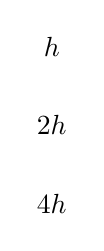
\begin{tikzpicture}
			\node   (h) at (-0.75, 4){$h$};
			\node   (2h) at (-0.75, 3){$2h$};
			\node   (4h) at (-0.75, 2){$4h$};
		\end{tikzpicture}
		\subcaption*{}
	\end{subfigure}
	\begin{subfigure}{0.22\textwidth}
		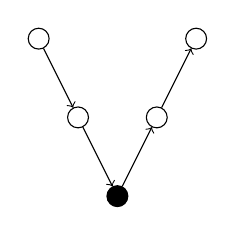
\begin{tikzpicture}
			\node	(a) at (0,4) [draw, circle,scale=0.8] {};
			\node	(b) at (0.5,3) [draw, circle,scale=0.8] {};
			\node	(c) at (1,2) [draw, circle,,fill=black,scale=0.8] {};
			\node	(d) at (1.5,3) [draw, circle,scale=0.8] {};
			\node	(e) at (2,4) [draw, circle, scale=0.8] {};
			
			\draw 
			(a) edge[->] (b) 
			(b) edge[->] (c)
			(c) edge[->] (d)
			(d) edge[->] (e)   
			;
		\end{tikzpicture}
		\subcaption*{$\gamma = 1$}
	\end{subfigure}
	\begin{subfigure}{0.32\textwidth}
		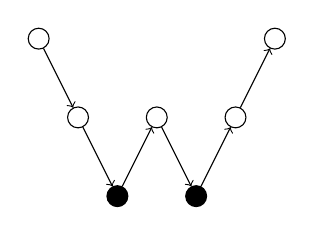
\begin{tikzpicture}
			\node	(a) at (0,4) [draw, circle,scale=0.8] {};
			\node	(b) at (0.5,3) [draw, circle,scale=0.8] {};
			\node	(c) at (1,2) [draw, circle,fill=black,scale=0.8] {};
			\node	(d) at (1.5,3) [draw, circle,scale=0.8] {};
			\node	(e) at (2,2) [draw, circle, fill=black, scale=0.8] {};
			\node	(f) at (2.5,3) [draw, circle, scale=0.8] {};
			\node	(g) at (3,4) [draw, circle, scale=0.8] {};
			
			\draw 
			(a) edge[->] (b) 
			(b) edge[->] (c)
			(c) edge[->] (d)
			(d) edge[->] (e)   
			(e) edge[->] (f)
			(f) edge[->] (g)
			;
		\end{tikzpicture}
		\subcaption*{$\gamma = 2$}
	\end{subfigure}
	\begin{subfigure}{0.32\textwidth}
		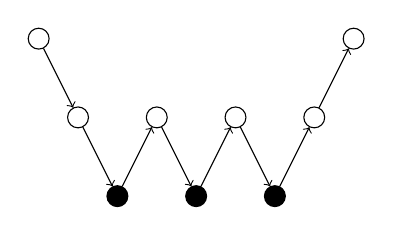
\begin{tikzpicture}
			\node	(a) at (0,4) [draw, circle,scale=0.8] {};
			\node	(b) at (0.5,3) [draw, circle,scale=0.8] {};
			\node	(c) at (1,2) [draw, circle,fill=black,scale=0.8] {};
			\node	(d) at (1.5,3) [draw, circle,scale=0.8] {};
			\node	(e) at (2,2) [draw, circle, fill=black, scale=0.8] {};
			\node	(f) at (2.5,3) [draw, circle, scale=0.8] {};
			\node	(g) at (3,2) [draw, circle, fill=black,scale=0.8] {};
			\node	(h) at (3.5,3) [draw, circle, scale=0.8] {};	
			\node	(i) at (4,4) [draw, circle, scale=0.8] {};	
			\draw 
			(a) edge[->] (b) 
			(b) edge[->] (c)
			(c) edge[->] (d)
			(d) edge[->] (e)   
			(e) edge[->] (f)
			(f) edge[->] (g)
			(g) edge[->] (h)
			(h) edge[->] (i)
			;
		\end{tikzpicture}
		\subcaption*{$\gamma = 3$}
	\end{subfigure}
	\caption{Three-grid cycles ($l = 2$).}
	\label{fig:three-grid-cycles}
\end{figure}
\begin{figure}
	\captionsetup{justification=centering}
	\begin{subfigure}{0.1\textwidth}
		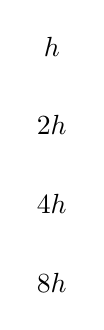
\begin{tikzpicture}
			\node   (h) at (-0.75, 4){$h$};
			\node   (2h) at (-0.75, 3){$2h$};
			\node   (4h) at (-0.75, 2){$4h$};
			\node   (8h) at (-0.75, 1){$8h$};
		\end{tikzpicture}
		\subcaption*{}
	\end{subfigure}
	\begin{subfigure}{0.3\textwidth}
		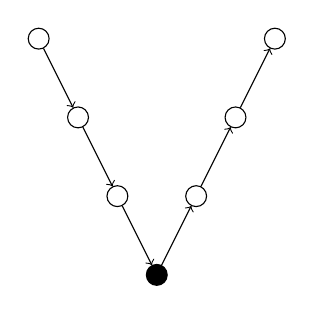
\begin{tikzpicture}
			\node	(a) at (0,4) [draw, circle,scale=0.8] {};
			\node	(b) at (0.5,3) [draw, circle,scale=0.8] {};
			\node	(c) at (1,2) [draw, circle,scale=0.8] {};
			\node	(d) at (1.5,1) [draw, circle,fill=black, scale=0.8] {};
			\node	(e) at (2,2) [draw, circle, scale=0.8] {};
			\node	(f) at (2.5,3) [draw, circle,scale=0.8] {};
			\node	(g) at (3,4) [draw, circle,scale=0.8] {};
			\draw 
			(a) edge[->] (b) 
			(b) edge[->] (c)
			(c) edge[->] (d)
			(d) edge[->] (e)   
			(e) edge[->] (f)
			(f) edge[->] (g)
			
			;
		\end{tikzpicture}
		\subcaption*{$\gamma = 1$}
	\end{subfigure}
	\begin{subfigure}{0.6\textwidth}
		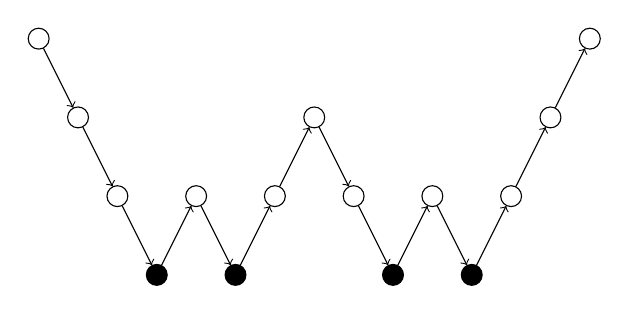
\begin{tikzpicture}
			\node	(a) at (0,4) [draw, circle,scale=0.8] {};
			\node	(b) at (0.5,3) [draw, circle,scale=0.8] {};
			\node	(c) at (1,2) [draw, circle,scale=0.8] {};
			\node	(d) at (1.5,1) [draw, circle,fill=black, scale=0.8] {};
			\node	(e) at (2,2) [draw, circle, scale=0.8] {};
			\node	(f) at (2.5,1) [draw, circle,fill=black,scale=0.8] {};
			\node	(g) at (3,2) [draw, circle,scale=0.8] {};
			\node	(h) at (3.5,3) [draw, circle,scale=0.8] {};
			\node	(i) at (4,2) [draw, circle,scale=0.8] {};
			\node	(j) at (4.5,1) [draw, circle,fill=black, scale=0.8] {};
			\node	(k) at (5,2) [draw, circle, scale=0.8] {};
			\node	(l) at (5.5,1) [draw, circle,fill=black,scale=0.8] {};
			\node	(m) at (6,2) [draw, circle,scale=0.8] {};
			\node	(n) at (6.5,3) [draw, circle, scale=0.8] {};
			\node	(o) at (7,4) [draw, circle, scale=0.8] {};
			
			\draw 
			(a) edge[->] (b) 
			(b) edge[->] (c)
			(c) edge[->] (d)
			(d) edge[->] (e)   
			(e) edge[->] (f)
			(f) edge[->] (g)
			(g) edge[->] (h)
			(h) edge[->] (i)
			(i) edge[->] (j)
			(j) edge[->] (k)
			(k) edge[->] (l)
			(l) edge[->] (m)
			(m) edge[->] (n)
			(n) edge[->] (o)
			;
		\end{tikzpicture}
		\subcaption*{$\gamma = 2$}
	\end{subfigure}
	\caption{Four-grid cycles ($l = 3$).}
	\label{fig:four-grid-cycles}
\end{figure}
Here each white node corresponds to one or multiple steps of smoothing on the respective level, while a black node implies that the resulting error equation is solved precisely.
Since, as it can be seen in Figure~\ref{fig:three-grid-cycles}, the choice of $\gamma = 1$ results in a V-shaped computational pattern, the corresponding multigrid method is usually called a V-cycle.
Similarly, the computational pattern of a method with $\gamma = 2$ on a three-grid hierarchy looks like a W, and hence the resulting method is called a W-cycle.
As it can be seen in Figure~\ref{fig:four-grid-cycles}, the amount of computational work within a W-cycle drastically increases with the number of coarsening steps.
While applying V-cycle always results in significantly fewer computations, in many cases, a single coarse grid correction step is not sufficient to reduce the low-frequency components of the initial error on the finest grid~\cite{trottenberg2000multigrid}.
Due to the resulting drastic increase in the number of computations, values of $\gamma$ larger than two are usually impractical for multigrid methods~\cite{trottenberg2000multigrid}.
While Algorithm~\ref{alg:multigrid-cycle} enables the construction of different multigrid methods based on choosing different values for the parameters $l$, $\gamma$, $\nu_1$, $\nu_2$ and $\omega$, the structural composition of the resulting methods is limited.
For instance, in Algorithm~\ref{alg:multigrid-cycle}, it is assumed that the same value of $\gamma$ is chosen on each level, which restricts possible computational patterns to those portrayed in Figure~\ref{fig:three-grid-cycles} and~\ref{fig:four-grid-cycles}.
One way to overcome this limitation is to combine different cycle types in a single method.
For instance, combining W- and V-cycles on each level results in a so-called F-cycle, whose algorithmic structure is illustrated by Figure~\ref{fig:f-cycle}.
\begin{figure}
	\begin{subfigure}{0.4\textwidth}
		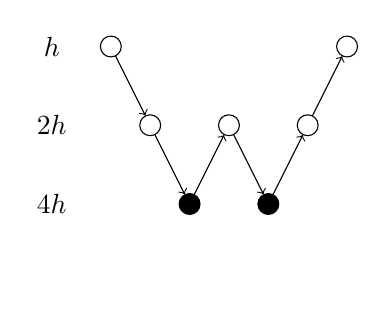
\begin{tikzpicture}
			\node   (h) at (-0.75, 4){$h$};
			\node   (2h) at (-0.75, 3){$2h$};
			\node   (4h) at (-0.75, 2){$4h$};
			\node   (8h) at (-0.75, 1){};
			\node	(a) at (0,4) [draw, circle,scale=0.8] {};
			\node	(b) at (0.5,3) [draw, circle,scale=0.8] {};
			\node	(c) at (1,2) [draw, circle,fill=black,scale=0.8] {};
			\node	(d) at (1.5,3) [draw, circle,scale=0.8] {};
			\node	(e) at (2,2) [draw, circle, fill=black, scale=0.8] {};
			\node	(f) at (2.5,3) [draw, circle, scale=0.8] {};
			\node	(g) at (3,4) [draw, circle, scale=0.8] {};
			
			\draw 
			(a) edge[->] (b) 
			(b) edge[->] (c)
			(c) edge[->] (d)
			(d) edge[->] (e)   
			(e) edge[->] (f)
			(f) edge[->] (g)
			;
		\end{tikzpicture}
	\end{subfigure}
	\begin{subfigure}{0.6\textwidth}
		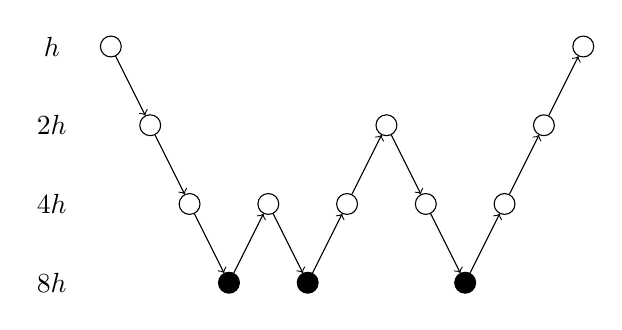
\begin{tikzpicture}
				\node   (h) at (-0.75, 4){$h$};
				\node   (2h) at (-0.75, 3){$2h$};
				\node   (4h) at (-0.75, 2){$4h$};
				\node   (8h) at (-0.75, 1){$8h$};
			\node	(a) at (0,4) [draw, circle,scale=0.8] {};
			\node	(b) at (0.5,3) [draw, circle,scale=0.8] {};
			\node	(c) at (1,2) [draw, circle,scale=0.8] {};
			\node	(d) at (1.5,1) [draw, circle,fill=black, scale=0.8] {};
			\node	(e) at (2,2) [draw, circle, scale=0.8] {};
			\node	(f) at (2.5,1) [draw, circle,fill=black,scale=0.8] {};
			\node	(g) at (3,2) [draw, circle,scale=0.8] {};
			\node	(h) at (3.5,3) [draw, circle,scale=0.8] {};
			\node	(i) at (4,2) [draw, circle,scale=0.8] {};
			\node	(j) at (4.5,1) [draw, circle,fill=black, scale=0.8] {};
			\node	(k) at (5,2) [draw, circle, scale=0.8] {};
			\node	(l) at (5.5,3) [draw, circle,scale=0.8] {};
			\node	(m) at (6,4) [draw, circle,scale=0.8] {};
			
			\draw 
			(a) edge[->] (b) 
			(b) edge[->] (c)
			(c) edge[->] (d)
			(d) edge[->] (e)   
			(e) edge[->] (f)
			(f) edge[->] (g)
			(g) edge[->] (h)
			(h) edge[->] (i)
			(i) edge[->] (j)
			(j) edge[->] (k)
			(k) edge[->] (l)
			(l) edge[->] (m)
			;
		\end{tikzpicture}
	\end{subfigure}
	\caption{Computational pattern of the F-cycle with a different number of coarsening steps.}
	\label{fig:f-cycle}
\end{figure}
Except for $l = 2$, in which case the F-cycle and W-cycle are equivalent, this method represents a compromise between a pure V-cycle and W-cycle.
While the composition of a multigrid method from different cycle types represents an additional degree of freedom, the individual cycles can still be formulated within the rules of Algorithm~\ref{alg:multigrid-cycle} and, hence, are fully described by the aforementioned parameters.
Since, according to the classical formulation of a multigrid method as in~\cite{brandt1977multi,hackbusch2013multi,trottenberg2000multigrid,briggs2000multigrid}, these parameters are considered global, adapting one of their values uniformly changes the method's behavior on each level. 
While for many applications, this approach has shown to yield efficient multigrid methods~\cite{trottenberg2000multigrid}, there are still cases where multigrid could not achieve its full potential~\cite{ernst2012difficult,benzi2005numerical}.
Even though, to date, there exists a rich amount of research on the optimization of multigrid cycles based on a fixed set of global parameters, the variation of its components on an individual level has not been considered yet.
Such an approach would grant the flexibility to generate multigrid cycles that consist of varying restriction and coarse-grid correction steps, each with a different combination of smoothers and relaxation factors.
In this work, we aim to realize this vision by expressing each multigrid cycle as a finite sequence of instructions whose order is restricted by the rules of linear algebra and multigrid theory.
To specify these rules in a mathematically formal way, we make use of programming language theory, such that the formulation of a multigrid method is treated as a program synthesis task.
In the next section, we, therefore, provide a brief overview of programming language theory and introduce the concept of formal languages and grammars.
We then combine this formalism together with our knowledge about multigrid methods to derive a novel representation of multigrid solvers that enables us to construct these methods in the form of a program design and optimization task.
\chapter{Formal Languages and Evolutionary Program Synthesis}
\label{chapter:formal-languages-and-gp}
  \section{Formal Languages and Grammars}
\label{sec:formal-languages}
In the previous section, we have introduced the theoretical background necessary to understand the fundamentals of multigrid methods.
The goal of this thesis is to develop a formal language that can express multigrid solvers of variable structure.
In general the \emph{alphabet} of a formal language is a non-empty set of symbols $\Sigma$.
Based on $\Sigma$ \emph{strings} can be created, which represent finite sequences of symbols.
For instance the alphabet $\Sigma = \left\{a, b\right\}$ contains only the symbols $a$ and $b$, as such $aabbb$ and $abaab$ are both strings on the alphabet $\Sigma$.
The length of a string, denoted by $|\cdot|$, is equal to the number of symbols contained in it. 
A concatenation of two strings 
\begin{equation}
	\begin{split}
		v & = a_1 a_2 \cdots a_n \\
		w & = b_1 b_2 \cdots b_m
	\end{split}
\end{equation}
is performed by appending the second string to the right of the first string such that
\begin{equation}
	vw = a_1 a_2 \cdots a_n b_1 b_2 \cdots b_m,
\end{equation}
The length of the concatenated string is then obviously equal to the sum of the length of the individual string, which means
\begin{equation}
|vw| = |v| + |w|.
\end{equation}
Finally, we define the empty string $\lambda$ as
\begin{equation}
	\begin{split}
		& |\lambda| = 0 \\
		& v \lambda = \lambda v = v,
	\end{split}
\end{equation}
where $v$ is a string on an arbitrary alphabet.
Assume $\Sigma$ is an alphabet, then $\Sigma^*$ is the set of strings obtained by concatenating zero or an arbitrary number of symbols from $\Sigma$.
Consequently, $\Sigma^*$ always contains the empty string $\lambda$.
To exclude $\lambda$ from the set, we define $\Sigma^+ = \Sigma^* \setminus \lambda$.
Since the number of strings that can be created from an alphabet through concatenation is infinite, both $\Sigma^+$ and $\Sigma^*$ represent infinite sets.
For example again let $\Sigma = \left\{a, b\right\}$ then
\begin{equation*}
	\Sigma^{*} = \left\{\lambda, a, b, aa, ab, ba, bb, aaa, aab, aba, \dots \right\}
\end{equation*} 
In general, for a given alphabet the \emph{language} $L$ is defined as a subset of $\Sigma^*$ (or $\Sigma^+$)
\begin{equation}
	L \supset \Sigma^*.
	\label{eq:language-basic-definition}
\end{equation}
However, in practice we usually want to obtain a language $L_G$ that represents a specific subset of $\Sigma^*$.
One way to achieve this is to define a set of rules that generate $L_G$.
These rules can be formally specified in form of a \emph{grammar}.
\begin{definition}[Grammar]
	\begin{equation*}
		G = \left(V, T, S, P \right),
	\end{equation*}
	where $V$ is a finite set of \emph{variables},
	$T$ a finite set of \emph{terminal symbols},
	$S \in V$ is the \emph{start} variable and 
	$P$ a finite set of \emph{productions} or \emph{production rules}.
	We also assume that $V \neq \emptyset$, $T \neq \emptyset$ and $V \cap T = \emptyset$.
\end{definition}
The core of a grammar are the productions $P$, which are usually specified as a set of mappings of the form
\begin{equation}
	x \to y,
	\label{eq:unrestricted-production}
\end{equation}
where $x \in \left(V \cup T\right)^+$ and $y \in \left(V \cup T\right)^*$.
Note that alternatively the operator
\begin{equation*}
	x \bnfpo y
\end{equation*}
is also often used to denote a production.
Each production rule $x \to y$ can then be applied in the following way.
Given a string $u$ of the form 
\begin{equation}
	u = vxw,
\end{equation}
we can replace $x$ with $y$ to \emph{derive} a new string
\begin{equation}
	u' = vyw,
\end{equation}
which is usually written as $u \Rightarrow u'$.
This process can then be continued by applying a sequence of derivations chosen arbitrarily from the set of available productions $P$.
Within this sequence each production can be applied whenever its conditions on the left-hand side of the rule are fulfilled, i.e. the respective pattern on occurs anywhere within the current string.
Also note that there is no limit on how many times a certain productions can be applied.
Each string $u$ at which we can arrive by applying an arbitrary sequence of productions starting from $S$
\begin{equation}
	S \Rightarrow \dots \Rightarrow u,
\end{equation}
is then an element of language $L_G$.
Assuming that 
\begin{equation}
	S \overset{*}{\Rightarrow} u.
\end{equation}
represents the application of an unspecified sequence of productions, we can define the language $L_G$ generated by the grammar $G$:
\begin{definition}[Language]\label{def:language}
	Let $G = \left\{V, T, S, P\right\}$ be a grammar, then
	\begin{equation}
		L_G = \left\{u \in T^* : S \overset{*}{\Rightarrow} u\right\}
	\end{equation}
is the language generated by $G$.
\end{definition}
Assuming $u \in L_G$ and 
\begin{equation}
	S \Rightarrow u_1 \Rightarrow u_2 \Rightarrow \dots \Rightarrow u_n \Rightarrow u
\end{equation}
is a \emph{derivation} of $u$, then the strings $S, u_1, u_2, \dots, u_n$ are called its \emph{sequential forms}.
\subsection{The Chomsky Hierarchy}
\label{sec:chomsky-hierarchy}
So far, we have not yet imposed any restrictions on the individual components of a grammar $G$.
We call such a grammar, whose productions are of the general form of Equation~\eqref{eq:unrestricted-production} \emph{unrestricted}.
In can be shown that any language generated by an unrestricted grammar is recursively enumerable, which means that there exists \emph{Turing machine} which is capable of enumerating all strings contained in that language~\cite{linz2006introduction}.
As a consequence, one can in fact prove that unrestricted grammars are equally powerful as Turing machines and, hence, both computational models are equivalent.
Since we are only interested in languages that possess this property and, hence, can be processed by any Turing-complete system on a modern computer, there is no use in considering languages that do not fall into this category.
While Turing machines and unrestricted grammars both represent an universal model of computation, it can be useful to consider grammars that impose certain restrictions on their productions and, hence, simplify both the derivation as well as the manipulation of strings.
\emph{Context-sensitive} grammars (CSG) represent a first step towards this direction.
\begin{definition}[Context-Sensitive Grammar]
A grammar $G = \left\{V, T, S, P\right\}$ is context-sensitive if all productions can be written as
\begin{equation*}
	xAy \to xuy
\end{equation*}
where $A \in V$ and $x, y, u \in \left(V \cup T\right)^*$.
\label{def:context-sensitive-grammar}
\end{definition}
This is equivalent to saying that a certain production $A \to u$ can only be peformed in the \emph{context} of $x$ and $y$, from which the term context-sensitive is derived.
While unrestricted grammars can be described by a Turing machine, the equivalent model of computation for a CSG is the \emph{linear bounded automaton}, which represents a Turing machine whose tape is linearly bounded by the length of the string~\cite{linz2006introduction}.
Furthermore, by prohibiting any context at the left-hand side of a production one arrives at the class of \emph{context-free} grammar (CFG).
\begin{definition}[Context-Free Grammar]
	A grammar $G = \left\{V, T, S, P\right\}$ is context-free if all productions are of the form
	\begin{equation*}
		A \to u 
	\end{equation*}
	where $A \in V$ and $u \in \left(V \cup T\right)^*$.
\end{definition}
The equivalent model of computation for a CFG is the \emph{pushdown automaton}~\cite{linz2006introduction}.  
CFGs have a number of desirable properties that justify their widespread use in computer science, especially in the theory of programming languages~\cite{pierce2002types}.
For instance, each string generated by a CFG as well as the derivation of each string can be represented as a tree.
Moreover, it is possible to check whether an arbitrary string of length $n$ is contained in the language generated by a CFG using only $\mathcal{O}(n^3)$ steps.
Note that the class of CFGs is contained in the class of CSGs, since we can simply replace each production 
\begin{equation}
	A \to u,
\end{equation}
of a CFG by one of the form
\begin{equation}
	xAy \to xuy,
\end{equation}
with $x = y = \lambda$. 
Since $\lambda \in \left(V \cup T\right)^*$, the resulting grammar meets the requirements of Definition~\ref{def:context-sensitive-grammar}.
Finally, the introduction of a further restriction on the productions leads to the class of regular grammars (RGs).
\begin{definition}[Regular Grammar]
	A grammar $G = \left\{V, T, S, P\right\}$ is regular if all productions are either of the form
	\begin{equation*}
		\begin{split}
			A & \to xB, \\
			A & \to x
		\end{split}
	\end{equation*}
in which case $G$ is said to be \emph{left-linear} or 
	\begin{equation*}
	\begin{split}
		A & \to Bx, \\
		A & \to x
	\end{split}
	\end{equation*}
in which case $G$ is said to be \emph{right-linear}, where in both cases $A, B \in V$ and $x \in T^*$.
\end{definition}
Since both $xB \in \left(V \cup T\right)^*$ and $Bx \in \left(V \cup T\right)^*$ it is obvious that each regular grammar can also be considered as a CFG.
Each language generated by a RG is a regular language and can, thus, be defined in form of a regular expression and, thus, they have the same expressive power as finite-state machines~\cite{linz2006introduction}.
With the definition of RGs we have arrived at the bottom of the so-called \emph{Chomsky hierarchy} of formal grammars and languages, which is given by the following set relations
\begin{equation*}
	\mathcal{G} \subset \mathcal{G}_{CS} \subset \mathcal{G}_{CF} \subset \mathcal{G}_{R}, 
\end{equation*} 
where $\mathcal{G}$ is the set of all unrestricted (type-0), $\mathcal{G}_{CS}$ the set of all context-sensitive (type-1), $\mathcal{G}_{CF}$ the set of all context-free (type-2) and $\mathcal{G}_{R}$ the set of all regular (type-3) grammars.
The same is true for the corresponding languages
\begin{equation*}
	\mathcal{L} \subset \mathcal{L}_{CS} \subset \mathcal{L}_{CF} \subset \mathcal{L}_{R}. 
\end{equation*}
Consequently, each level in this hierarchy corresponds to a particular class of grammars introduced in this section, where each subsequent level introduces further restrictions on the productions but on the other hand enables the use of faster and more efficient algorithms for manipulating the strings contained in its generated language.
After we have now introduced a class of formal languages for representing strings of symbols in a structured way as well as those grammars able to generate them, we next discuss how we can represent the construction and manipulation of such strings as a combinatorial search problem, whose solution we aim to approximate using randomized population-based search methods.







   


  \section{Genetic Programming}
\emph{Genetic Programming} (GP) is a class of search algorithms for finding optimal programs based on the principle of natural evolution first proposed by John Koza~\cite{koza1994genetic}.
In general, a program $p$ can be considered as a mapping from the set of inputs $\mathcal{I}$ to the corresponding set of outputs $\mathcal{O}$
\begin{equation}
	p : \mathcal{I} \to \mathcal{O}.
\end{equation}
However, since not all input-output pairs are known in advance, this mapping is usually given in form of a finite set of training cases.
The goal of GP is then to find a program that correctly computes the correct output for each input contained in the training set.
Since there is often not a unique program that satisfies this condition, usually a number of additional constraints are applied to assess the quality of each correct program.
For instance, in practice one is often interested in finding the shortest or fastest program that is able to pass all training cases.
Based on a program's effectiveness in solving all training cases under the given constraints, GP then assigns a \emph{fitness} value to each program, which is then treated as an \emph{individual} within a \emph{population} of programs.
In evolutionary computation, the population is a set of individuals currently considered within the search and, therefore, spans a subspace within the space of solutions for the given search problem.
Each subsequent step of the search is then performed by generating a new population based on the previous one through \emph{mutation} or recombination (often called \emph{crossover}) of the individuals contained in the current one.
Usually, the candidates for mutation and crossover are sampled from the current population based on the fitness value computed for each individual.
If we repeat this procedure for a number of $n$ steps, we arrive at a final population $P_n$, which can then additionally be evaluated on a test set, to obtain the best overall program.
The resulting search method is summarized in Algorithm~\ref{alg:genetic-programming}. 
\begin{algorithm}[t]
	\caption{Genetic Programming}
	\label{alg:genetic-programming}
	\begin{algorithmic} % The number tells where the line numbering should start
		\State \textbf{Randomly generate} an initial population $P_0$ of programs
		\State \textbf{Evaluate} $P_0$ on the \textbf{training set} 
		\For{$i := 1, \dots, n$}
		\State \textbf{Select} a subset of individuals $M_i \supset P_{i-1}$ based on their \textbf{fitness}
		\State \textbf{Generate} new programs $C_i$ based on $M_i$ using \textbf{mutation} and \textbf{crossover}
		\State \textbf{Evaluate} $C_i$ on the \textbf{training set} 
		\State \textbf{Select} $P_{i}$ from $C_i \cup P_{i-1}$
		\EndFor
		\State \textbf{Evaluate} the final population $P_{n}$ on a \textbf{test set}  to obtain the best overall program
	\end{algorithmic}
\end{algorithm}
While Algorithm~\ref{alg:genetic-programming} gives an overview of the general structure of a GP method, we have not yet considered how the individual operations such as the generation of an initial population and the creation of new individuals through mutation and crossover can be performed.
Since all these operations are based on manipulating the internal structure of a given program, the first step in the implementation of a GP method choosing a suitable program representation.
Note that this representation does not necessarily need to be equal to the target language in which the actual program is supposed to be implemented but rather needs to define a unique mapping that enables its automatic generation.
This process is usually called \emph{genotype} to \emph{phenotype} mapping, where the genotype refers to the internal representation used within GP while the phenotype then represents the actual program implemented on the target machine.
One of the most widely used genotype representations is tree-based GP, where each program is internally represented as a tree of expressions, which was also initially proposed by John Koza~\cite{koza1994genetic}.
While within the last decades numerous other GP variants have been proposed~\cite{poli2008field}, such as grammatical evolution~\cite{o2001grammatical}, linear GP~\cite{brameier2007linear} and cartesian GP~\cite{miller2008cartesian}, we focus on tree-based GP as it forms the basis for our implementation, which will be presented in later chapters.
\section{Representation}
In contrast to other evolutionary algorithms algorithms, which usually represent the solution to an optimization problem as an array of discrete or continuous numbers~\cite{back1997handbook}, GP deals with the optimization of programs and, hence, each solution corresponds to an executable program.
%Before we consider these operations in detail, we first need to define a procedure to generate program expression trees in a structured way. 
For this purpose, we consider the following context-free grammar $G$ with the productions
\begin{equation}
	\begin{split}
		S & \to E \\
		E & \to \text{if} \; B \; \text{then} \; E \; \text{else} \; E \; | \; A \\
		A & \to -A \; | \; (A + A) \; | \; (A - A) \; | \; (A \cdot A) \; | \; A^A \; | \; x \; | \; y \\  
		B & \to \neg B \; | \; (B \wedge B) \; | \; (B \vee B) \; | \; u \; | \; v,
	\end{split}
\label{eq:gp-example-grammar}
\end{equation}
where $V = \{S, E, A, B\}$ is the set of variables and the symbols $x$, $y$ represent numbers while the symbols $u$, $v$ correspond to boolean values, i.e. $\top$ or $\bot$.
If we treat $x$, $y$, $u$ and $v$ as an input, each expression generated by $G$ can be considered as a quaternary function $f(x,y,u,v) \in L_{G}$, where $L_G$ is the language generated by $G$ according to Definition~\ref{def:language}.
For example the functions
\begin{equation}
	\begin{split}
		f_1(x,y,u,v) & = \text{if} \; (\neg u \wedge v) \; \text{then} \; (x \cdot x) \; \text{else} \; (x / y) \\
		f_2(x,y,u,v) & = x^{(x + y)} - (y \cdot y)
	\end{split}
\label{eq:gp-example-functions}
\end{equation} can both be generated by $G$ and are, hence, included in $L_G$.
By applying the rules of arithmetic and boolean algebra, we can compute the result of each such function based on a given set of inputs.
Therefore, assuming both $x$ and $y$ represent real-valued numbers, we can evaluate the correctness of the mapping $f : x, y, u, v \to \mathbb{R}$ for an arbitrary number of test cases.
Next, to define suitable operations for generating arbitrary functions $f \in L_G$, we need to choose a suitable data structure for its representation.
While a program's structure depends on the programming language it is formulated in, in many cases it is possible to formulate it as a tree of program expressions, which is especially true for languages from the Lisp-family, that have been originally employed in John Koza's work~\cite{koza1994genetic}.
In tree-based GP all operations are performed on program expression trees and, thus, both mutation and crossover must be designed with respect to this representation.
Expression trees can be created in a straightforward way after rewriting each expression in postfix notation. 
To obtain the corresponding tree, the expressions is traversed sequentially by putting each operand that either represents a terminal symbol or has been already transformed on a stack and then retrieving those operands from the top of the stack for each new operator encountered.
Figure~\ref{fig:gp-expression-tree-examples} shows the corresponding expression trees for $f_1$ and $f_2$.
\begin{figure}
	\begin{subfigure}{0.59\textwidth}
		\includegraphics{figures/gp_tree1.pdf}
	\end{subfigure}
	\begin{subfigure}{0.41\textwidth}
		\includegraphics{figures/gp_tree2.pdf}
	\end{subfigure}
 \caption{Expression trees for $f_1$ and $f_2$, where we have simplified the if-then-else construct to a single ternary operator.}
 \label{fig:gp-expression-tree-examples}
\end{figure}
On the other hand, given a certain expression tree, we can easily restore the original expression by traversing the tree recursively in a top-down manner while generating the corresponding expression for each node as soon as each of its operands has been recursively processed or in case it is available as a terminal symbol.
While expression trees can be both easily generated from a given program, as well as offering an efficient way to evaluate a certain program, they possess an inherent limitation, which is the absence of type information.
For a better understanding of this, we reconsider the context-free grammar formulated in Equation~\eqref{eq:gp-example-grammar}.
Therein all productions on the variable $B$ only result in the generation of boolean expressions, while all productions starting from $A$ exclusively lead to arithmetic expressions.
As a consequence, we are not allowed to intermix expressions that are derived from $A$ and $B$.
However, this information is not contained in any of the expressions generated by $G$ and, hence, also missing in the corresponding tree.
As the generation of each new expression can be performed based on the productions of $G$, it is guaranteed to be valid.
However, the main step of GP is the creation of new individuals based on the existing ones in the population either through recombination of two individuals (crossover) or by altering certain parts of a given individual (mutation). 
Both operations require us to investigate which nodes and subtrees of a given expression trees can be safely replaced by an alternative branch without violating the type constraints imposed within the productions of our grammar.
While it is possible to deal with this problem by simply evicting those individuals that violate any type constraints from the population, depending on the number of constraints, this will be the case for a high percentage of individuals, leading to a highly inefficient method.
A different and usually more efficient approach is to annotate each node within an expression tree with additional type information, which leads to the concept of strongly-typed GP, first proposed by David Montana~\cite{montana1995strongly}.
Strongly-typed GP represents a viable solution to the problem of retaining type correctness, but it requires us to transform the implicit type information contained within the productions of our grammar into explicit type annotations at the nodes of each expression tree.
As an alternative we can instead utilize the information encoded in the productions of a grammar $G$ by considering the \emph{derivations} of an expression $e \in L_G$, as defined by
\begin{equation}
	S \Rightarrow e_1 \Rightarrow e_2 \Rightarrow \dots \Rightarrow e_n \Rightarrow e.
\end{equation}
If $G$ is context-free each of its possible derivations can be represented as a tree, where the root node is always the start variable $S$ and each level of the tree corresponds to a sequential form $e_i$ within the derivation~\cite{linz2006introduction}.
%Furthermore, if $G$ is regular, its derivations can be further simplified to finite state machine, where each state corresponds to a sequential form. 

\chapter{A Formal Language for Multigrid Methods}
\label{chapter:multigrid-formal-language}
  After establishing a theoretical foundation both about multigrid methods and evolutionary grammar-based optimization techniques, the first primary goal of this thesis is to develop a formal language for expressing arbitrarily structured multigrid solvers in a generalized way.
For this purpose, first observe that the multigrid solvers described Section~\ref{sec:multigrid-cycles} can be all classified by their \emph{cycle type}.
Each such cycle possesses a distinct computational pattern which stems from the number of recursive descents performed on each level of the method.
For instance a V-cycle is characterized by exactly one recursive descent per level.
All these classically considered multigrid cycles employ a fixed uniform number of recursive descents and smoothing steps per discretization level, which is determined by the parameters $\gamma$, $\nu_1$ and $\nu_2$ in Algorithm~\ref{alg:multigrid-cycle}.
While the representation of a multigrid method as a recursive cycle yields a formally simple and easily parameterizable algorithmic formulation it also enforces unnecessary restrictions on its structure.
Consider for instance the multigrid method depicted in Figure~\ref{fig:non-traditional-multigrid-cycle}.
\begin{figure}
	\begin{subfigure}{0.1\textwidth}
		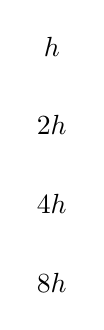
\begin{tikzpicture}
			\node   (h) at (-0.75, 4){$h$};
			\node   (2h) at (-0.75, 3){$2h$};
			\node   (4h) at (-0.75, 2){$4h$};
			\node   (8h) at (-0.75, 1){$8h$};
		\end{tikzpicture}
	\end{subfigure}
	\begin{subfigure}{0.9\textwidth}
		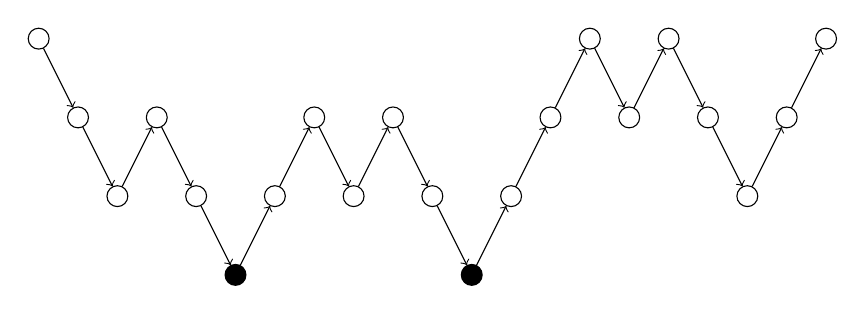
\begin{tikzpicture}
			\node	(a) at (0,4) [draw, circle,scale=0.8] {};
			\node	(b) at (0.5,3) [draw, circle,scale=0.8] {};
			\node	(c) at (1,2) [draw, circle,scale=0.8] {};
			\node	(d) at (1.5,3) [draw, circle, scale=0.8] {};
			\node	(e) at (2,2) [draw, circle, scale=0.8] {};
			\node	(f) at (2.5,1) [draw, circle,scale=0.8,fill=black] {};
			\node	(g) at (3,2) [draw, circle,scale=0.8] {};
			\node	(h) at (3.5,3) [draw, circle,scale=0.8] {};
			\node	(i) at (4,2) [draw, circle,scale=0.8] {};
			\node	(j) at (4.5,3) [draw, circle,scale=0.8] {};
			\node	(k) at (5,2) [draw, circle,scale=0.8] {};
			\node	(l) at (5.5,1) [draw, circle,scale=0.8,fill=black] {};
			\node	(m) at (6,2) [draw, circle,scale=0.8] {};
			\node	(n) at (6.5,3) [draw, circle,scale=0.8] {};
			\node	(o) at (7,4) [draw, circle,scale=0.8] {};
			\node	(p) at (7.5,3) [draw, circle,scale=0.8] {};
			\node	(q) at (8,4) [draw, circle,scale=0.8] {};
			\node	(r) at (8.5,3) [draw, circle,scale=0.8] {};
			\node	(s) at (9,2) [draw, circle,scale=0.8] {};
			\node	(t) at (9.5,3) [draw, circle,scale=0.8] {};
			\node	(u) at (10,4) [draw, circle,scale=0.8] {};
			\draw 
			(a) edge[->] (b) 
			(b) edge[->] (c)
			(c) edge[->] (d)
			(d) edge[->] (e)   
			(e) edge[->] (f)
			(f) edge[->] (g)
			(g) edge[->] (h)
			(h) edge[->] (i)
			(i) edge[->] (j)
			(j) edge[->] (k)
			(k) edge[->] (l)
			(l) edge[->] (m)
			(m) edge[->] (n)
			(n) edge[->] (o)
			(o) edge[->] (p)
			(p) edge[->] (q)
			(q) edge[->] (r)
			(r) edge[->] (s)
			(s) edge[->] (t)
			(t) edge[->] (u)
			;
		\end{tikzpicture}
	\end{subfigure}
	\caption{Example for a non-traditional multigrid method.}
	\label{fig:non-traditional-multigrid-cycle}
\end{figure}
While this method reaches the coarsest level twice and, hence, at first sight looks similar to a W-cycle, it employs a unique pattern of computations that is completely different from those of any of the traditional multigrid cycles.
As a consequence, this method can not be represented within the classical framework of multigrid cycles, as formulated in Algorithm~\ref{alg:multigrid-cycle}.
To overcome these limitations and construct multgrid methods with an arbitrary sequence of computations on each discretization level, as illustrated by the example in Figure~\ref{fig:non-traditional-multigrid-cycle}, a new formal language for their representation is needed.
The first step towards the development of this language is to find a way to represent the current state within each step of a multigrid method and then define transition rules between those states.

\section{Multigrid States}
\label{}
In order to determine how the state of a multigrid method can be represented, we need to reconsider our original formulation of a multigrid cycle in Algorithm~\ref{alg:multigrid-cycle}.
The sake of simplicity, in the following we write symbols that correspond to vectors also in regular font.
In case the mathematical interpretation of a certain lower case symbol is ambiguous, its meaning will be explicitly stated. 
On each level $l > 0$ only the following three operations are employed within a multgrid cycle.
\begin{description}
	\item[Smoothing:] Reduce the oscillatory error components of the approximate solution $\tilde{x}_h$ on the current level. 
	\begin{equation*}
		\tilde{x}_h = \tilde{x}_h + \omega M_h^{-1} \left( b_h - A_h \tilde{x}_h \right) \; \text{where} \; A_h = M_h + N_h
	\end{equation*}
	\item[Restriction:] Restrict the residual to obtain the right-hand side $b_{2h}$ of the error equation on the next coarser level.
	\begin{align*}
		\tilde{x}_{2h} & = 0 \\
 		b_{2h} & = I_h^{2h} (b_h - A_h \tilde{x}_h)
	\end{align*}
	\item[Coarse-Grid Correction:] Prolongate a correction $\tilde{x}_{2h}$ obtained on a coarser grid to reduce the low-frequency error components of the approximate solution $\tilde{x}_h$.
	\begin{equation*}
		\tilde{x}_h = \tilde{x}_h + I_{2h}^h \tilde{x}_{2h}
	\end{equation*}
\end{description}
Now note that except for the operators $A_h$, $I_h^{2h}$ and $I_{2h}^h$ the result of each of these operations exclusively depends on the current value of the approximate solution on subsequent levels, i.e. $\tilde{x}_{h}$ and $\tilde{x}_{2h}$, and the right-hand side $b_h$.
However, in contrast to coarse-grid correction which utilizes the current approximate solution on the coarse grid, both smoothing and restriction first compute the residual $r_h = b_h - A_h \tilde{x}_h$, which can be considered as an intermediate step.
While this differentiation is not strictly necessary it leads to simpler operations, since both restriction and smoothing can then be split into two steps.
Furthermore, as in practice the actual error can usually not be computed, the residual is often the only available metric to investigate whether a multigrid iteration has achieved a certain amount of error reduction and, hence, has to be repeatedly computed.
%The residual is then either restricted and assigned to the right-hand side $b_{2h}$ or employed to reduce the oscillatory error components of the approximate solution by computing a correction term of the form $\omega A_h^{-1} r_h$.
To derive a general representation for the state of a multigrid method based on our previous observations, we consider the sequence of operations shown in Algorithm~\ref{alg:example-three-grid-method}, which corresponds to a three-grid V-cycle that performs one step of underrelaxed Jacobi smoothing on the second finest level.
\begin{algorithm}
	\begin{algorithmic}[1]
		\State $\tilde{x}_{h} = x_{h}^0$
		\State $r_{h} = b_{h} - A_h \tilde{x}_{h} $
		\State $ \tilde{x}_{2h} = 0$
		\State $ b_{2h} = I_{h}^{2h} r_{h}$
		\State $ r_{2h} = b_{2h} - A_{2h} \tilde{x}_{2h}$
		\State $ \tilde{x}_{2h} = \tilde{x}_{2h} + I_{4h}^{2h} A_{4h}^{-1} I_{2h}^{4h} r_{2h}$
		\State $ r_{2h} = b_{2h} - A_{2h} \tilde{x}_{2h}$
		\State $ \tilde{x}_{2h} = \tilde{x}_{2h} + 0.6 \cdot D_{2h}^{-1} r_{2h}$
		\State $\tilde{x}_{h} = \tilde{x}_{h}  + I_{2h}^h \tilde{x}_{2h}$
	\end{algorithmic}
\caption{Example for a three-grid V-cycle}
\label{alg:example-three-grid-method}
\end{algorithm}
In each step of this sequence of operations either the approximate solution, right-hand side or residual is updated on a certain level.
While in practice each of these variables corresponds to a data structure encompassing numerical values, our goal is to represent the algorithmic structure of a multigrid solver in the form of symbolic expressions.
In this case the value of each variable is determined by the expression that computes its value.
Updating a variable, therefore, corresponds to assigning a new expression to the corresponding symbol.
For this purpose, we consider the tuple
\begin{equation*}
	S_h = (\tilde{x}_h, b_h, r_h)
\end{equation*} 
on each level with step size $h$, which then contains expression of each of the corresponding three variables.
Starting from the first line we can then progressively update the contents of this tuple with the expression contained in each line, whereby the occurrence of each symbol is replaced by the respective expression currently contained in the tuple.
Figure~\ref{fig:example-tree-grid-method-states} shows the respective state tuple for each line of Algorithm~\ref{alg:example-three-grid-method}.
\begin{figure}
	\begin{equation*}
		\begin{array}{l l l}
			\hline
			\bm{S_h} & \bm{=} & \bm{(\tilde{x}_h, \, b_h, \, r_h)}  \\
			1: & &  x_{h}^0, \, b_h, \, \lambda \\
			2: & &  x_{h}^0, \, b_h, \, b_{h} - A_h x_{h}^0 \\ \hline
			\bm{S_{2h}} & \bm{=} &  \bm{(\tilde{x}_{2h}, \, b_{2h}, \, r_{2h})} \\
			3: & &  0, \, \lambda, \, \lambda \\
			4: & &  0, \, I_{h}^{2h}\underbrace{(b_{h} - A_h x_{h}^0)}_{r_{h}}, \, \lambda \\
			5: & &  0, \, I_{h}^{2h}(b_{h} - A_h x_{h}^0), \,\underbrace{I_{h}^{2h}(b_{h} - A_h x_{h}^0)}_{b_{2h}} - A_{2h} 0 \\
			6: & & 0 + I_{4h}^{2h} A_{4h}^{-1} I_{2h}^{4h} (\underbrace{I_{h}^{2h}(b_{h} - A_h x_{h}^0) - A_{2h} 0}_{r_{2h}}), \, I_{h}^{2h}(b_{h} - A_h x_{h}^0), \, \lambda\\
			7: & & 0 + I_{4h}^{2h} A_{4h}^{-1} I_{2h}^{4h} (I_{h}^{2h}(b_{h} - A_h x_{h}^0) - A_{2h} 0), \, I_{h}^{2h}(b_{h} - A_h x_{h}^0), \\ 
			& &  \underbrace{I_{h}^{2h}(b_{h} - A_h x_{h}^0)}_{b_{2h}} - A_{2h} (\underbrace{0 + I_{4h}^{2h} A_{4h}^{-1} I_{2h}^{4h} (I_{h}^{2h}(b_{h} - A_h x_{h}^0) - A_{2h} 0)}_{\tilde{u}_{2h}}) \\
			8: & &   (\underbrace{0 + I_{4h}^{2h} A_{4h}^{-1} I_{2h}^{4h} (I_{h}^{2h}(b_{h} - A_h x_{h}^0) - A_{2h} 0)}_{\tilde{u}_{2h}}) + 0.6 \cdot D_{2h}^{-1} \cdot \\ 
			& & (\underbrace{I_{h}^{2h}(b_{h} - A_h x_{h}^0) - A_{2h} (0 + I_{4h}^{2h} A_{4h}^{-1} I_{2h}^{4h} (I_{h}^{2h}(b_{h} - A_h x_{h}^0) - A_{2h} 0))}_{r_{2h}}), \\ 
			& & I_{h}^{2h}(b_{h} - A_h x_{h}^0), \, \lambda \\ \hline 
			\bm{S_h} & \bm{=} & \bm{(\tilde{x}_h, \, b_h, \, r_h)}  \\
			9: & & x_{h}^0 + I_{2h}^h ((0 + I_{4h}^{2h} A_{4h}^{-1} I_{2h}^{4h} (I_{h}^{2h}(b_{h} - A_h x_{h}^0) - A_{2h} 0)) + 0.6 \cdot D_{2h}^{-1} \cdot \\ 
			& &  (I_{h}^{2h}(b_{h} - A_h x_{h}^0) - A_{2h} (0 + I_{4h}^{2h} A_{4h}^{-1} I_{2h}^{4h} (I_{h}^{2h}(b_{h} - A_h x_{h}^0) - A_{2h} 0)))), \\ 
			& &  b_h, \, \lambda \\
			\hline
		\end{array}
	\end{equation*}
	\caption{State tuple in each step of Algorithm~\ref{alg:example-three-grid-method}.}
	\label{fig:example-tree-grid-method-states}
\end{figure}
As it has been introduced in Section~\ref{sec:formal-languages}, the empty symbol $\lambda$ denotes that a certain component of the tuple is unspecified.
After the last step of the sequence (line 9) the first component of the tuple ($\tilde{x}_h$) then combines all computational steps of the method in a single expression.

While Figure~\ref{fig:example-tree-grid-method-states} illustrates that the ternary tuple contains all relevant information of a multigrid method's current state on a certain level, we have not yet considered how to transition between the states of two subsequent levels.
First, consider the case of transitioning from a certain level with step size $h$ to the next coarser level with step size $2h$, which is shown in line 3 and 4 of Figure~\ref{fig:example-tree-grid-method-states}.
Here the tuple
\begin{equation*}
	S_{2h} = (0, \, I_{h}^{2h}(b_{h} - A_h x_{h}^0), \, \lambda)
\end{equation*} 
corresponds to the coarse-grid error equation 
\begin{equation*}
	A_{2h} x_{2h} = I_{h}^{2h}(b_{h} - A_h x_{h}^0),
\end{equation*}
whose solution is to be approximated starting with an initial guess of zero.
Therefore, all information to create this state is obtained from the next finer level in form of the restricted residual $I_h^{2h} r_h = I_h^{2h} (b_{h} - A_h x_{h}^0)$.
On the other hand, consider the transition from a coarse grid back to the next finer grid in form of the coarse-grid correction in line 9.
In this case we both require the approximate solution $\tilde{x}_{2h}$, computed on the coarse grid, as well as the previous values of the first two components $\tilde{x}_h$ and $b_h$ of the fine-grid state tuple.
While in the case of restriction we can neglect all previous states represented on the coarser grid, as it is explicitly contained in the residual, for a coarse-grid correction the previous state on the fine-grid needs to be restored.
Note that in case of a multigrid method that operates on a hierarchy of discretizations of even larger depth than the example shown in Algorithm~\ref{alg:example-three-grid-method}, this process must be recursively performed for each bottom up transition within the hierarchy.
To resolve this issue we need to extend our original formulation of a multgrid state by a fourth component with the purpose of preserving current state of the next finer level.
While at the topmost level this component is always empty, whenever restriction is performed the state of the current level is included.
For instance in line 4 of Figure~\ref{fig:example-tree-grid-method-states} we have to extend the given ternary tuple 
\begin{equation*}
S_{2h} = (0, \, I_{h}^{2h}(b_{h} - A_h x_{h}^0), \, \lambda)
\end{equation*}
by including the state 
\begin{equation*}
S_h = (x_{h}^0, \, b_h, \, b_{h} - A_h x_{h}^0, \, \lambda) 
\end{equation*} 
as an additional fourth entry. 
Hence, all required information for restoring the previous fine-grid state values is then included in the quaternary tuple 
\begin{equation*}
	S_{2h} = (0, \, I_{h}^{2h}(b_{h} - A_h x_{h}^0), \, \lambda, \, S_h).
\end{equation*}
%TODO clarify that line 3 and 4 can in practice be combined to one step
Note that since $S_h$ represents the current state on the finest grid, its fourth component is empty, while otherwise it would refer to the previous state of the next higher level in the discretization hierarchy.
To assess the feasibility of this approach, we have to check whether all components required to construct the coarse-grid correction expression, as in line 9 of Figure~\ref{fig:example-tree-grid-method-states}, are available within the current state.
However, since in addition to $\tilde{x}_{2h}$, both the approximate solution $\tilde{x}_h$ and right-hand side $b_h$ are now contained in the fourth component of the coarse-grid state tuple, this expression can be assembled in a straightforward manner.
At this point, it should be noted that coarse-grid correction from the coarsest grid represents a special case. 
Since the only allowed operation on this level is the application of the coarse-grid solver, which is denoted by a multiplication with the inverse of the system matrix, it is represented as a single operation in form of the expression 
\begin{equation*}
	\tilde{x}_{2h} = \tilde{x}_{2h} + I_{4h}^{2h} A_{4h}^{-1} I_{2h}^{4h} r_{2h}.
\end{equation*}
After resolving the issue of restoring previous states during coarse-grid correction, we can, thus, now provide a complete formal definition of the state of a multigrid method.
\begin{definition}[Multigrid State]
\label{def:multigrid-state}
The state of a multigrid method for solving the equation $A_{2h} x_{2h} = b_{2h}$ on a certain grid with step size $2h$ is given by the quaternary tuple
\begin{equation*}
	S_{h} = \left( \tilde{x}_{h}, b_{h}, c_{h}, S_{h}\right), 
\end{equation*}
where
\begin{itemize}
	\item $\tilde{x}_{h}$ is a mathematical expression for computing an approximate solution of the above equation,
	\item $b_{h}$ is an expression for computing the right-hand side of the above equation,
	\item $c_{h}$ is a correction term for improving the accuracy of the approximate solution,
	\item $S_{h/2}$ is either the current state on the next finer level with a step size $h/2$ or the empty symbol $\lambda$ in case $h$ represents the topmost level in the given hierarchy of discretizations.
\end{itemize}
\end{definition}
Note that in Definition~\ref{def:multigrid-state} the third component $c_{2h}$ of a multigrid state no longer only refers to the residual, but now represents an expression that corresponds to a general correction term.
While in the classical multigrid formulation, as presented in Section~\ref{sec:multigrid-methods}, all smoothing expressions are directly derived from the residual, alternative relaxation methods which can not be easily formulated in the simple framework of stationary iterative methods, such as distributive smoothing, have been proposed~\cite{trottenberg2000multigrid}.
Furthermore, the general notion of a correction term enables us to also represent intermediate expressions that do not specifically refer to the current residual within a multigrid state, for instance $c_h = \omega M_h^{-1} \left( b_h - A_h \tilde{x}_h \right)$ which corresponds to the complete term that is added to the current approximate solution within smoothing.   
%Finally, note that the computation of the coarse-grid correction does not require the value of the previous fine-grid residual.
%Therefore, the corresponding expression does not need to be restored and the residual can be omitted in the respective state tuple when performing the fine-to-coarse grid transition.
\section{State Transition Rules}
After defining the state of a multigrid method, the next step towards developing a formal language for representing arbitrary sequences of multigrid operations,
such as the one shown in Figure~\ref{fig:non-traditional-multigrid-cycle}, is to formally define a set of rules that describes the transitions between all possible states.
For this purpose, we need to consider the set of possible operations within a multigrid method, as described at the beginning of the last section.
From a mathematical point of view, these operations exclusively consist of either matrix-vector multiplications or vector additions and subtractions.
First of all, the computation of the residual $r_h = b_h - A_h \tilde{x}_h$ represents the fundamental operation based on which an approximation to the solution of the target system $A_h x_h = b_h$ is iteratively improved, either with means of smoothing or by computing a coarse-grid correction.
The \textsc{residual} function implements the corresponding state transition for computing the residual on a certain level with step size $h$.
For this purpose first the residual expression is assembled based on the system matrix $A_h$ and the given state $S_h = (\tilde{x}_h, b_h, \lambda, S_{h/2})$, which contains the current approximate solution $\tilde{x}_h$ and right-hand side $b_h$.
The resulting expression is included as a the correction term $c_h$ into $S_h$, which is then returned at the end of the function.
%TODO describe residual
%TODO include references to functions
\begin{algorithm}
	\begin{algorithmic}
		\Function{residual}{$A_h$, $(\tilde{x}_h, b_h, \lambda, S_{h/2})$}
		\State $c_h \gets b_h - A_h \tilde{x}_h$
		\State return $(\tilde{x}_h, b_h, c_h, S_{h/2})$
		\EndFunction
	\end{algorithmic}
\label{alg:state-transition-residual}
\end{algorithm}
After constructing an initial correction $c_h$ from the residual expression $b_h - A_h \tilde{x}_h$, next we can apply an operator $B_h$ to this term, either as part of a smoothing expression or in form of restriction to obtain the right-hand side $b_h$ of the coarse-grid error equation.
Since both operations can be formulated as a matrix-vector multiplication, we consider this operator application as an intermediate step that is implemented in form of the function \textsc{apply}.
This function applies to operator $B_h$ to the current correction term. 
The resulting expression then serves as a new correction term within the returned state.
\begin{algorithm}
	\begin{algorithmic}
		\Function{apply}{$B_h$, $(\tilde{x}_h, b_h, c_h, S_h)$}
		\State return $(\tilde{x}_h, b_h, B_h\cdot c_h, S_h)$
		\EndFunction
	\end{algorithmic}
\end{algorithm}
In general, the choice of the operator $B_h$ corresponds to the two elementary options available within a multigrid method, i.e. smoothing and solving the given problem on a coarser grid.
For instance, the choice of $B_h = D_h^{-1}$ leads to the expression
\begin{equation*}
	c_h = D_{-1} (b_h - A_h \tilde{x}_h),
\end{equation*}
which corresponds to one step of the Jacobi method as shown in Equation~\ref{eq:jacobi-method}.
In contrast, choosing $B_h$ as the restriction operator $I_h^{2h}$ leads to
\begin{equation*}
	c_{2h} = I_{h}^{2h} (b_h - A_h \tilde{x}_h),
\end{equation*}
which then serves as a right-hand side $b_{2h}$ of the corresponding coarse-grid error equation.
In both cases the correction term obtained from the \textsc{apply} function serves a different purpose.
First of all, we must be able to generate an expression that computes an improved approximate solution $\tilde{x}_h$ by applying an update in form of the correction term $c_h$ to the previous value of $\tilde{x}_h$. 
This behavior is implemented in the function \textsc{iterate}, which returns a state tuple with the expression for computing an updated approximate solution as its first entry.
In addition to the mere application of a correction term, this function also includes a relaxation factor $\omega$ and partitioning operator $P$ which enables both the formulation of underrelaxed, overrelaxed and potentially colored versions of each operation, for instance those described in Section~\ref{sec:rb-gs}.
The second possibility to apply an operator to the current residual is in form of the restriction expression $c_{2h} = I_{h}^{2h} r_h$.
As denoted by the subscript, the result of this operation represents an expression on a coarser grid of step size $2h$.
To construct the coarse-grid error equation $A_{2h} x_{2h} = I_{h}^{2h} r_h$ we have to assign this expression to the right-hand side $b_{2h}$ within the corresponding state tuple.
Furthermore, as discussed within the last section, before we can transition to a state on the next coarser grid, we have to store the previous state as a fourth component in the corresponding tuple.
The resulting state transition is implemented in the function \textsc{cge}, which is abbreviation of the term coarse-grid equation.
\begin{algorithm}
	\begin{algorithmic}
		\Function{cge}{$A_{2h}$, $x_{2h}^0$, ($\tilde{x}_h$, $b_{h}$, $c_{2h}$, $S_{h/2}$)}
		\State $\tilde{x}_{2h} \gets 0$ 
		\State $b_{2h} \gets c_{2h}$
		\State $c_{2h} \gets b_{2h} - A_{2h} \tilde{x}_{2h}$ 
		\State $S_h \gets$ ($\tilde{x}_{2h}$, $b_{h}$, $\lambda$, $S_{h/2}$)
		\State return ($\tilde{x}_{2h}$, $b_{2h}$, $c_{2h}$, $S_h$)
		\EndFunction
	\end{algorithmic}
\end{algorithm}
Note that within this function we already construct an expression for the initial residual
\begin{equation}
	r_{2h} = b_{2h} - A_{2h} 0,
\end{equation} 
and include it as a correction term into the newly created state tuple.
Performing a coarse-grid correction with the initial approximate solution $0$ does not lead to any improvement, and, thus, computing the residual always represents the first step of solving the coarse-grid error equation with subsequent multigrid operations.
Finally, after deriving an expression $\tilde{x}_{2h}$ for computing the approximate solution of the error equation on the coarse grid, we have to transfer this term back to the fine grid, where it can then be applied as a correction to the current approximate solution on this level.
For this purpose we first need to restore the previous state on the next finer level including the current approximate solution, right-hand side and, in case this state does not represent the topmost level within the discretization level, also its predecessor state.
To obtain the coarse-grid expression expression we then need to apply the prolongation operator to the current approximate solution on the coarse-grid.
The resulting state transition is implemented in the function \textsc{cgc}.
Note that the complete coarse-grid correction step is then obtained through subsequent application of the \textsc{iterate} function, which updates the approximate solution with the correction term obtained within \textsc{cgc}.
\begin{algorithm}
	\begin{algorithmic}
		\Function{cgc}{$I_{2h}^{h}$, ($\tilde{x}_{2h}$, $b_{2h}$, $\lambda$, $S_{h}$)}
		\State ($\tilde{x}_h$, $f_{h}$, $c_h$, $S_{h/2}$) $\gets S_{h}$
		\State $c_h \gets I_{2h}^{h} \cdot \tilde{x}_{2h}$
		\State return ($\tilde{x}_h$, $f_{h}$, $c_h$, $S_{h/2}$)
		\EndFunction
	\end{algorithmic}
\end{algorithm}
%TODO describe coarse-grid solver A_{4h}^{-1}
As it has been described in this section, the application of each of these functions corresponds to a certain transition between the possible states of a multigrid solver, and, hencce, for every possible multigrid method a sequence of function applications can be assembled.
The evaluation of this sequence then leads to a state whose first component $\tilde{x}_h$ contains an expression that corresponds to the step wise execution of all steps of the method.
The functions described in this section can therefore be considered as a \textsc{language} for the formal description of multigrid methods.
At this point we also have to revisit one of the main goals of this language: The description of methods that incorporate an arbitrary sequence of multigrid operations and, thus, can not be formulated in the classical framework of multigrid cycles, as shown in Algorithm~\ref{alg:multigrid-cycle}.
As we have described in this section, we have ensured that each possible state transition within a multigrid method is described by the application of either a specific combination of functions or even a single one.
However, we have carefully avoided to introduce functions that correspond to a transition spanning over multiple states, which would reduce the expressiveness of our language, and, thus, similar to Algorithm~\ref{alg:multigrid-cycle}, restrict it to only a subset of all possible multigrid methods.
The remaining step within the development of a formal system for the construction of arbitrary sequences of multigrid operations is, thus, the derivation of a formal grammar that generates the corresponding strings contained in our multigrid language, as it has been described in Section~\ref{sec:formal-languages}.
\section{Multigrid Grammar}
In Section~\ref{sec:formal-languages} we have already introduced the definition of a general grammar $G$ as the quaternary tuple 
\begin{equation*}
	G = \left(V, T, S, P \right),
\end{equation*}
where $V$ is the set of variables, $T$ the set of terminal symbols, $S \in V$ the start symbol and $P$ the set of productions.
However, before we start defining a grammars individual components, the question arises whether it is necessary to impose additional restrictions on its structure.
As it has been discussed in Section~\ref{sec:chomsky-hierarchy}, the Chomsky hierarchy defines four grammatical levels, where each subsequent level introduces additional constraints on a grammar's structure.
While an unrestricted or type-0 grammar represents the most general model of computation, it also leads to the highest degree of complexity.
In particular, for each language $L_G$ generated by an unrestricted grammar there exists a Turing-machine that is able to decide whether a certain string $w$ is contained in $L_G$.
However, in case $w \notin L_G$ it is impossible to ensure that this procedure will always end in a finite number of steps, which can, hence, result in infinite loop.
\begin{algorithm}
	\begin{bnf*}
		\bnfprod{$S$} {
			\bnfpn{$s_h$}
		} \\
		\bnfprod{$s_h$} {
			\bnfts{\textnormal{\textsc{iterate}}}(\bnfts{\textnormal{\textsc{apply}}}(\bnfpn{$B_h$}, \bnfsp \bnfpn{$c_h$}), \bnfsp \bnfts{$\omega$}, \bnfsp \bnfpn{$P$}) \bnfor
		} \\
		\bnfmore {
			\bnfts{\textnormal{\textsc{iterate}}}(\bnfts{\textnormal{\textsc{cgc}}}(\bnfts{$I_{2h}^h$}, \bnfsp \bnfpn{$s_{2h}$}), \bnfsp \bnfts{$\omega$}, \bnfsp \bnfpn{$P$}) \bnfor (\bnfts{$x_h^0$}, \bnfsp \bnfts{$b_h$},\bnfsp \bnfes, \bnfsp \bnfes)
		} \\
		\bnfprod{$c_h$} {
			\bnfts{\textnormal{\textsc{residual}}}(\bnfts{$A_h$}, \bnfsp \bnfpn{$s_h$}) 
		} \\
		\bnfprod{$B_h$} {
			\bnfts{\textnormal{\textsc{inverse}}}(\bnfts{$A_h^{+}$}) \bnfsp \bnfts{\textnormal{with}} \bnfsp \bnfts{$A_{h} = A_{h}^{+} + A_{h}^{-}$}
		} \\ \\
		\bnfprod{$s_{2h}$} {
			\bnfts{\textnormal{\textsc{iterate}}}(\bnfts{\textnormal{\textsc{apply}}}(\bnfpn{$B_{2h}$}, \bnfsp \bnfpn{$c_{2h}$}), \bnfsp \bnfts{$\omega$}, \bnfsp \bnfpn{$P$}) \bnfor
		} \\
		\bnfmore {
			\bnfts{\textnormal{\textsc{iterate}}}(\bnfts{\textnormal{\textsc{cgc}}}(\bnfts{$I_{4h}^{2h}$}, \bnfsp \bnfpn{$s_{4h}$}), \bnfsp \bnfts{$\omega$}, \bnfsp \bnfpn{$P$})
			%\bnfts{\textnormal{\textsc{iterate}}}(\bnfts{\textnormal{\textsc{apply}}}(\bnfts{$I_{4h}^{2h}$}, \bnfsp \bnfpn{$c_{4h}$}), \bnfsp \bnfts{$\omega$}, \bnfsp \bnfes)
		} \\
		\bnfprod{$c_{2h}$} {
			\bnfts{\textnormal{\textsc{residual}}}(\bnfts{$A_{2h}$}, \bnfsp \bnfpn{$s_{2h}$}) \bnfor 			\bnfts{\textnormal{\textsc{cge}}}(\bnfts{$A_{2h}$}, \bnfsp \bnfts{$0_{2h}$}, \bnfsp \bnfts{\textnormal{\textsc{apply}}}(\bnfts{$I_h^{2h}$}, \bnfsp \bnfpn{$c_h$}))
		} \\
		\bnfprod{$B_{2h}$} {
			\bnfts{\textnormal{\textsc{inverse}}}(\bnfts{$A_{2h}^{+}$}) \bnfsp \bnfts{\textnormal{with}} \bnfsp \bnfts{$A_{2h} = A_{2h}^{+} + A_{2h}^{-}$}
		} \\ \\
		\bnfprod{$s_{4h}$} {
			\bnfts{\textnormal{\textsc{iterate}}}(\bnfts{\textnormal{\textsc{apply}}}(\bnfpn{$B_{4h}$}, \bnfsp \bnfpn{$c_{4h}$}), \bnfsp \bnfts{$\omega$}, \bnfsp \bnfpn{$P$})
		} \\
		\bnfmore {
			\bnfts{\textnormal{\textsc{iterate}}}(\bnfts{\textnormal{\textsc{cgc}}}(\bnfts{$I_{8h}^{4h}$}, \bnfsp \bnfpn{$s_{8h}$}), \bnfsp \bnfts{$\omega$}, \bnfsp \bnfpn{$P$})
			%\bnfts{\textnormal{\textsc{iterate}}}(\bnfts{\textnormal{\textsc{apply}}}(\bnfts{$I_{4h}^{2h}$}, \bnfsp \bnfpn{$c_{4h}$}), \bnfsp \bnfts{$\omega$}, \bnfsp \bnfes)
		} \\
		\bnfprod{$c_{4h}$} {
			\bnfts{\textnormal{\textsc{residual}}}(\bnfts{$A_{4h}$}, \bnfsp \bnfpn{$s_{4h}$}) \bnfor 			\bnfts{\textnormal{\textsc{cge}}}(\bnfts{$A_{4h}$}, \bnfsp \bnfts{$0_{4h}$}, \bnfsp \bnfts{\textnormal{\textsc{apply}}}(\bnfts{$I_{2h}^{4h}$}, \bnfsp \bnfpn{$c_{2h}$}))
		} \\
		\bnfprod{$B_{4h}$} {
			\bnfts{\textnormal{\textsc{inverse}}}(\bnfts{$A_{4h}^{+}$}) \bnfsp \bnfts{\textnormal{with}} \bnfsp \bnfts{$A_{4h} = A_{4h}^{+} + A_{4h}^{-}$}
		} \\ \\
		\bnfprod{$s_{8h}$} {
			\bnfts{\textnormal{\textsc{iterate}}}(\bnfts{\textnormal{\textsc{apply}}}(\bnfpn{$B_{8h}$}, \bnfsp \bnfpn{$c_{8h}$}), \bnfsp \bnfts{$\omega$}, \bnfsp \bnfpn{$P$})
		} \\
		\bnfmore {
			\bnfts{\textnormal{\textsc{iterate}}}(\bnfts{\textnormal{\textsc{apply}}}(\bnfts{$I_{16h}^{8h}$}, \bnfsp \bnfpn{$c_{16h}$}), \bnfsp \bnfts{$\omega$}, \bnfsp \bnfes)
		} \\
		\bnfprod{$c_{8h}$} {
			\bnfts{\textnormal{\textsc{residual}}}(\bnfts{$A_{8h}$}, \bnfsp \bnfpn{$s_{8h}$}) \bnfor 			\bnfts{\textnormal{\textsc{cge}}}(\bnfts{$A_{8h}$}, \bnfsp \bnfts{$0_{8h}$}, \bnfsp \bnfts{\textnormal{\textsc{apply}}}(\bnfts{$I_{4h}^{8h}$}, \bnfsp \bnfpn{$c_{4h}$}))
		} \\
		\bnfprod{$B_{8h}$} {
			\bnfts{\textnormal{\textsc{inverse}}}(\bnfts{$A_{8h}^{+}$}) \bnfsp \bnfts{\textnormal{with}} \bnfsp \bnfts{$A_{8h} = A_{8h}^{+} + A_{8h}^{-}$}
		} \\ \\
		\bnfprod{${c}_{16h}$} {
			\bnfts{\textnormal{\textsc{apply}}}(\bnfts{$A^{-1}_{16h}$}, \bnfsp \bnfts{\textnormal{\textsc{apply}}}(\bnfts{$I_{8h}^{16h}$}, \bnfsp \bnfpn{$c_{8h}$}))
		} \\
		\bnfprod{$P$} {
			\bnfts{\textnormal{\textsc{partitioning}}} \bnfor \bnfes
		}
	\end{bnf*}
\label{alg:multigrid-grammar}
\caption{Grammar Productions for a Five-Grid Method}
\end{algorithm}


\chapter{The EvoStencils Framework -- Part 1: Core Implementation}
\label{chapter:evostencils-1}
  \usemintedstyle{tango}
\setminted[python]{fontsize=\footnotesize, breaklines}
%\setminted[scala]{fontsize=\footnotesize, breaklines}
In the first part of this thesis, we have established a theoretical foundation for multigrid methods, formal languages, and evolutionary program synthesis.
In Chapter~\ref{chapter:multigrid-formal-language}, building on this foundation, we have then developed a novel formal language and grammar for the automatic generation of multigrid methods. 
While we have already demonstrated the capabilities of this approach in alternating each individual step of a multigrid method, we could not yet demonstrate its benefits compared to the use of classical multigrid cycles, such as V-, F-, and W-cycles.
We aim to achieve this goal with the implementation of \emph{EvoStencils}, a prototypical Python framework for the automated grammar-based design of multigrid methods.
Using this framework, we will show how it is possible to discover novel methods that are able to solve certain PDE-based problems faster than all classical multigrid cycles.
However, before we discuss EvoStencils' features and their implementation in Python, we want to provide an overview of its general workflow and software architecture.
Here, we distinguish between EvoStencils' core implementation and the functionality of the framework that builds upon external libraries.
Since we have expressed the rules our multigrid construction rules in the form of a context-free grammar, we can apply the evolutionary program synthesis techniques presented Chapter~\ref{chapter:formal-languages-and-gp} without significant adaptions.
For this purpose, we employ the widely-used evolutionary computation framework DEAP\footnote{DEAP: \url{https://github.com/deap/deap}}~\cite{rainville2012deap}, which enables us to implement grammar-guided genetic programming (G3P) in a modular way.
However, we then need to address the question of how we can evaluate each multigrid method obtained through G3P in an automatic and reproducible manner.
As we have seen in Section~\ref{sec:grammar-based-algorithm-generation} the 
execution of the sequence of state transition functions contained in a given derivation tree produces a computational graph in the form of Figure~\ref{fig:example-three-grid-method-computational-graph}.
This graph can then be translated to an algorithmic representation, as demonstrated by Algorithm~\ref{alg:example-three-grid-method-generated}.
However, while a domain expert could manually implement the corresponding multigrid solver based on this representation using a numerical software package, our framework has to perform the evaluation of each method in an automatic way without requiring any human intervention.
Recently, code-generation techniques that only require the specification of a numerical solver in a high-level domain-specific language (DSL) have become increasingly powerful~\cite{kostler2020code}.
An example of this approach is the ExaStencils framework~\cite{lengauer2020exastencils,lengauer2014exastencils}, which has been specifically designed for the automatic generation of fast and scalable implementations of multigrid-based solvers specified in a tailored DSL called ExaSlang~\cite{schmitt2014exaslang,schmitt2016systems,kuckuk2016automatic}.
ExaSlang allows to represent a multigrid method as a sequence of high-level operations while granting the user the flexibility to apply further optimizations through the addition of code transformations and lower-level statements.
To evaluate a given solver obtained from a grammar-based representation, we emit its corresponding algorithmic formulation as an ExaSlang specification, based on which we then generate a scalable C++ implementation using the capabilities of the ExaStencils framework.
The resulting program can then be executed on a number of test cases in order to measure its desired performance characteristics.
Finally, note that the execution of an evolutionary program synthesis approach requires the evaluation of a large number of different multigrid methods.
Depending on the problem that one aims to solve, it can be infeasible to run this method on a single compute node, which necessitates a multi-node parallelization.
The message passing interface (MPI)~\cite{walker1996mpi} provides a unified interface for performing parallel computations on a distributed system that is supported by the majority of available supercomputing devices.
While MPI was originally designed for the traditional scientific computing languages Fortran and C, it has recently been made available within Python~\cite{dalcin2021mpi4py}. 
With the addition of MPI as a distributed computing backend, we arrive at the following high-level view of EvoStencils' software architecture, which is shown in Figure~\ref{fig:evostencils-architecture}.
\begin{figure}
	\resizebox{\columnwidth}{!}{%
		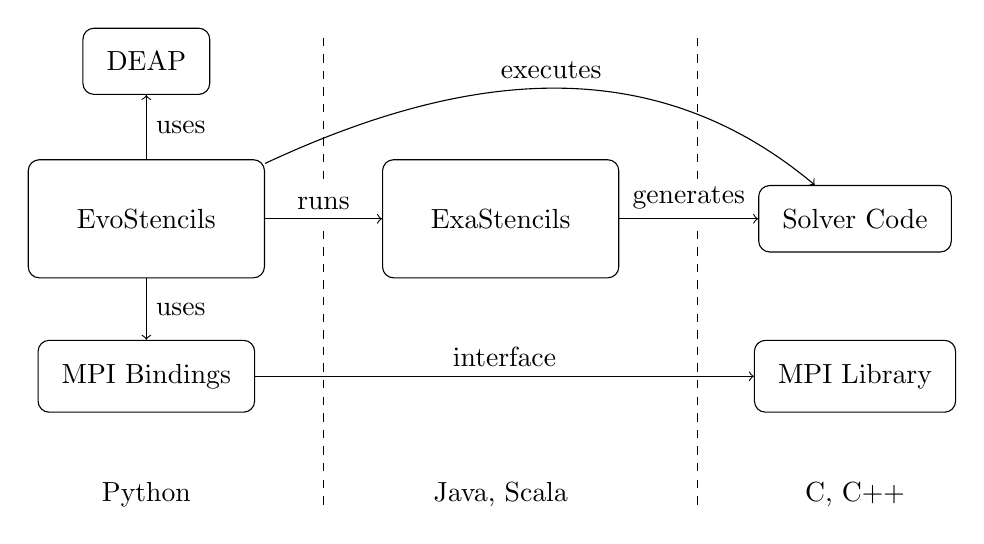
\begin{tikzpicture}
			%\draw [help lines] (-10,-10) grid (10,10);
			\node[draw, minimum width=3cm, minimum height=1.5cm, rounded corners] (evo) at (0,0) {EvoStencils};
			\node[draw, inner sep=3mm, rounded corners] (bindings) at (0, -2) {MPI Bindings};
			\node[draw, inner sep=3mm, rounded corners] (deap) at (0, 2) {DEAP};
			\node[draw, minimum width=3cm, minimum height=1.5cm, rounded corners] (exa) at (4.5, 0) {ExaStencils};
			\node[draw, inner sep=3mm, rounded corners] (code) at (9, 0) {Solver Code};
			\node[draw, inner sep=3mm, rounded corners] (mpi) at (9, -2) {MPI Library};
			\draw[dashed] (2.25, 2.3) -- (2.25,0.5);
			\draw[dashed] (2.25, -0.15) -- (2.25,-3.7);
			\draw[dashed] (7, 2.3) -- (7,0.5);
			\draw[dashed] (7, -0.15) -- (7,-3.7);
			\node (python) at (0, -3.5) {Python};
			\node (java) at (4.5, -3.5) {Java, Scala};
			\node (c) at (9, -3.5) {C, C++};
			\draw[->] (evo)-- node[anchor=west] {uses} (deap);
			\draw[->] (evo)-- node[anchor=south]{runs} (exa);
			\draw[->] (exa)--node[anchor=south] {generates} (code);
			\draw[->] (evo) to [out=25,in=140] node[anchor=south] {executes} (code);
			\draw[->] (bindings)--node[anchor=south] {interface}(mpi);
			\draw[->] (evo)--node[anchor=west] {uses}(bindings);
			%\draw[->] (mpi)--(code);
		\end{tikzpicture}
	}\caption{Software Architecture of EvoStencils.}
	\label{fig:evostencils-architecture}
\end{figure}
In the following, we will now discuss the individual parts of this architecture in more detail, starting with the core implementation of EvoStencils, which can be considered as a separate module that does not depend on any of the other tools and libraries mentioned here.
As a first step, we will outline the implementation of an intermediate representation (IR) for multigrid methods that can be generated in a straightforward manner based on a given derivation tree.
This IR will then acts as a basis for all subsequent steps of solver generation and evaluation.

\section{Intermediate Representation}
\label{sec:intermediate-representation}
Before we can derive an actual representation of multigrid methods comprising their computational structure, we need to be aware of the fact that all operations of a multigrid method are defined on a grid with a certain step size.
%Note that algebraic multigrid methods~\cite{stuben2001introduction,ruge1987algebraic}, which are not considered in this work, represent an exception to this, as they operate on sparse matrix data structures.
In Section~\ref{sec:discretization} we have already made the assumption of discretizing the underlying PDE on a hierarchy of structured grids.
To identify a grid within this hierarchy, certain information is required, which we store in a \emph{Grid} data structure whose implementation is shown in Listing~\ref{code:ir:grid}.
In general, a structured grid is defined by its size, i.e., the number of grid points and spacing $h$ in each dimension.
In addition, we also include the grid's level to identify it within the discretization hierarchy.
Note that in case the grid is uniform, we only need to store a single value for its spacing in each dimension, while otherwise, a value would need to be stored for each pair of grid points.
As the problems considered in this work are all solved on a hierarchy of uniform grids, we focus on this particular case.
\begin{listing}
	\inputminted{python}{evostencils/ir/grid.py}
	\caption{IR: Structured Grid}
	\label{code:ir:grid}
\end{listing}
After defining a data structure that provides all relevant information about a certain grid within the discretization hierarchy, we can start defining expressions that operate on this data structure.
For this purpose, in Listing~\ref{code:ir:abstact-base-class}, a common abstract base class is provided from which all subsequent expression classes are derived.
\begin{listing}
	\inputminted{python}{evostencils/ir/expression.py}
	\caption{IR: Abstract Expression Base Class}
	\label{code:ir:abstact-base-class}
\end{listing}
In addition to the already mentioned grid data structure, this class also defines a \emph{shape} for each expression.
From a mathematical point of view, each expression contained in a multigrid method either computes a matrix or a vector whose shape can be derived recursively from its operands.
The shape of the corresponding expression is then defined as a pair $(r, c)$, whose first entry $r$ corresponds to the number of rows and the second $c$ to the number of columns, which in the given example is both $m$.
Based on this abstract class, we can then further distinguish between predefined entities, such as the system matrix and right-hand side, and expressions that refer to the mathematical operations of a multigrid method.
First of all, Listing~\ref{code:ir:entity} contains the implementation of the entity base class.
\begin{listing}
	\inputminted{python}{evostencils/ir/entity.py}
	\caption{IR: Entity Base Class}
	\label{code:ir:entity}
\end{listing}
In addition to the previously mentioned attributes, this class is also given a \emph{name} to identify the respective entity.
Based on this implementation, we can then further define classes for representing an approximate solution, right-hand side and operator, which are shown in the Listings~\ref{code:ir:approximation} and~\ref{code:ir:operator}.
\begin{listing}
	\inputminted{python}{evostencils/ir/approximation.py}
	\caption{IR: Approximate Solution and Right-Hand Side}
	\label{code:ir:approximation}
\end{listing}
\begin{listing}
	\inputminted{python}{evostencils/ir/operator.py}
	\caption{IR: Operator}
	\label{code:ir:operator}
\end{listing}
In these cases, the shape of the respective entity is obtained by computing the grid size product across all dimensions, whereas in the case of the approximation and right-hand side, the result can be considered as a vector, whereas the shape of an operator corresponds to a quadratic matrix.
Since the \emph{Approximation} and \emph{RightHandSide} classes, from a mathematical point of view, can be both considered as a vector, we only implement the former and then make use of inheritance to avoid unnecessary code duplication.
In addition to the attributes defined in its parent class, an \emph{Approximation} includes a \emph{predecessor} attribute, whose meaning will be discussed later when we construct the actual grammar.
While the other two entities discussed here correspond to the solution and right-hand side of a discretized PDE, Listing~\ref{code:ir:operator} represents its operator, given as one or multiple stencil codes.
In Section~\ref{subsec:stencil-codes}, we have already introduced a mathematical notation for stencil codes in the form of Equation~\eqref{eq:stencil-definition}, which can be implemented in the Python programming language in a straightforward manner leading to the \emph{Stencil} class shown in Listing~\ref{code:ir:stencil}.
%TODO introduce stencil implementation here
\begin{listing}
	\inputminted{python}{evostencils/ir/stencil.py}
	\caption{IR: Stencil}
	\label{code:ir:stencil}
\end{listing}
The \emph{entries} attribute of this class directly corresponds to the set $S_h$ defined in Equation~\ref{eq:stencil-definition}, whereby we use a \emph{tuple} object to represent this set in the Python programming language.
Each entry $e_i$ of this object then again represents a tuple of the form of
\begin{equation}
	e_i = \left(\bm{a}_i, b_i \right),
\end{equation} 
where $\bm{a}_i$ is the offset from the current grid point in each dimension, given as an array of integer values, and $b_i$ is the stencil value that corresponds to each offset, given as a floating point number.
Based on this class, we can then provide implementations for all operations on stencil codes that have been defined in Section~\ref{subsec:stencil-codes}.
%Furthermore, in accordance with Section~\ref{subsec:systems-of-pdes} and~\ref{subsec:block-smoothing}, we can extend this implementation to systems of PDEs and block smoothers, which will be briefly covered in the next Chapter of this thesis. %TODO insert ref to next chapter here or remove sentence
Now note that in our implementation of the \emph{Operator} class in Listing~\ref{code:ir:operator} the stencil is not included directly, but instead, we provide a so-called \emph{stencil generator}.
A stencil generator is a function that returns the discretization of an operator on a particular grid in the form of a stencil.
For instance, the finite-difference discretization of the Laplace operator $\nabla^2$ on a two-dimensional uniform grid leads to the stencil 
\begin{equation*}
	\begin{split}
		\Delta_{h,h} = & \; \big\{ \left( \left( 0,0 \right), 4 / h^2 \right), \left(\left(1,0\right), -1/h^2\right), \left(\left(-1,0\right), -1 / h^2\right), \\ & \left(\left(0,1\right), -1/h^2\right), \left(\left(0,-1\right), -1/h^2\right) \big\}_{h,h}.
	\end{split}
\end{equation*}
in which the value at each offset depends on the grid spacing $h$.
Furthermore, in certain cases, it is possible to construct the higher-dimensional version of a stencil from its lower-dimensional counterparts, as we have shown in Section~\ref{subsec:restriction-and-prolongation} for the considered prolongation and restriction operators.
Therefore, instead of storing a unique stencil for each individual operator instance, we can parametrize its generation based on the features of the applied discretization by including a reference to the respective generator function.
Finally, as both prolongation and restriction transfer information between adjacent grids within a hierarchy of discretizations, they can be considered as a special case of an operator, which, for instance, leads to a different value of the \emph{shape} attribute.
For this purpose, the class \emph{InterGridOperator}, from which all restriction and prolongation operators are derived, extends the \emph{Operator} class with the required functionality.
For the sake of brevity, the implementation of this class and the respective \emph{Restriction} and \emph{Prolongation} subclasses can be found in Section~\ref{appendix:ir} of the appendix.

After discussing the implementation of the different entities upon which a multigrid method is built, we next shift our attention to the implementation of IR classes for representing the expressions that constitute its computational structure. 
For this purpose, we first provide basic classes for representing unary and binary expressions, which are shown in the Listings~\ref{code:ir:unary-expression} and~\ref{code:ir:binary-expression}.
\begin{listing}
	\inputminted{python}{evostencils/ir/unary_expression.py}
	\caption{IR: Unary Expression Base Class}
	\label{code:ir:unary-expression}
\end{listing}
\begin{listing}
	\inputminted{python}{evostencils/ir/binary_expression.py}
	\caption{IR: Binary Expressions Base Class}
	\label{code:ir:binary-expression}
\end{listing}
In both cases, all necessary properties are obtained from the expression's operands in a recursive manner.
However, since the result of a binary expression depends on the type of operation, we raise an error if this method is not implemented in one of the derived classes. 
To illustrate that the majority of multigrid operations can already be expressed based on these two classes, we have included a number of specific examples in Section~\ref{appendix:ir} of the appendix.
As discussed in Section~\ref{sec:grammar-based-algorithm-generation}, we aim to represent the computational structure of a given multigrid method as a redundancy-free directed graph. 
While the previously defined base classes allow us to represent the arithmetic expressions that occur within the correction terms of a multigrid method, there are two operations that require special treatment.
As we have already seen in Figure~\ref{fig:example-three-grid-method-computational-graph} it is necessary to access previously computed intermediate results on multiple occasions within a multigrid method.
In particular, each time a coarse-grid correction is performed, we have to restore the previous approximate solution and right-hand side on the respective level.
Furthermore, whenever we compute a new residual, the current expression for both the right-hand side and approximate solution is required.
For this purpose, we implement the classes \emph{Residual} and \emph{Cycle}, which allow us to establish additional references to previously defined expressions within a multigrid method.
Each of these references then corresponds to one of the subgraphs in Figure~\ref{fig:example-three-grid-method-computational-graph} with root nodes that possess multiple incoming edges, i.e., those subgraphs that have been annotated in Figure~\ref{fig:example-three-grid-method-computational-graph-annotated}.
We will later see how these references can be utilized to construct a complete graph from the grammar-based representation of a multigrid method.
Listing~\ref{code:ir:residual} shows the implementation of the \emph{Residual} class, which contains references to the system operator $A_H$ and the expressions for computing the current approximate solution $\tilde{x}_H$ and right-hand side $b_H$, where $H$ is the grid spacing on the current level.
Based on these components, we can easily construct the corresponding residual expression $r_H = b_H - A_H \tilde{x}_H$.
\begin{listing}
	\inputminted{python}{evostencils/ir/residual.py}
	\caption{IR: Residual}
	\label{code:ir:residual}
\end{listing}
As a final step in the implementation of our intermediate representation, the definition of the \emph{Cycle} class can be found in Listing~\ref{code:ir:cycle}.
\begin{listing}
	\inputminted{python}{evostencils/ir/cycle.py}
	\caption{IR: Multigrid Cycle}
	\label{code:ir:cycle}
\end{listing}
This class represents one step of computing a new value for the approximate solution $\tilde{x}_H$ on a particular level with spacing $H$, i.e.,
\begin{equation}
	\tilde{x}_H = \tilde{x}_H + \omega c_H \; \text{with} \; P,
\end{equation}
where $c_H$ is a correction term, $\omega$ the relaxation factor and $P$ a partitioning.
To make the right-hand side available in subsequent steps of the method, such as for the computation of the residual, the data structure includes an additional reference to the corresponding object.
Additionally, a reference to the previous state on the next-higher level is needed to restore the expression for the approximate solution and right-hand side after applying a coarse-grid correction.
To better understand the purpose of these two classes, consider the example shown in Listing~\ref{code:ir:example.py}, which demonstrates the construction of a computational graph based on the IR described in this section.
\begin{listing}
	\inputminted{python}{evostencils/ir/example.py}
	\caption{Example Usage of the Intermediate Representation}
	\label{code:ir:example.py}
\end{listing}
Starting on the original problem on the finest grid, we first store references to the initial approximate solution and right-hand side in a \emph{Cycle} object, which itself is included as a \emph{predecessor} reference in the subsequently created coarse-grid \emph{Cycle} object.
In order to apply the latter as a coarse-grid correction on the finest grid, the original fine-grid \emph{Cycle} object is restored, and its \emph{correction} variable is replaced by the respective expression, which is obtained by applying the prolongation operator to the approximate solution that has been previously computed on the coarse grid.
As this example demonstrates, our IR enables us to assemble the computational graph of a multigrid method in a stepwise manner.
However, to automate the process of generating a multigrid method from its grammar-based representation, we must be able to translate any sequence of derivations into a corresponding IR object.
For this purpose, we will utilize the functionality of the evolutionary computation framework DEAP~\cite{rainville2012deap}.
However, before we proceed with this task, we want to address some final remarks about the IR presented in this section.
The main purpose of the implementation presented here is to uniquely represent the computational structure of a multigrid method in the form of a redundancy-free directed graph.
Thus, to be able to construct such a graph in a step-wise manner based on the formal system described in Chapter~\ref{chapter:multigrid-formal-language}, each \emph{Cycle} node needs to include additional references to the current approximate solution and right-hand side.
While this information is important for the construction of the graph, it could later be discarded by replacing each such node with the respective arithmetic expression for computing an updated approximate solution, as it is shown in the \textsc{update} function in Section~\ref{sec:multigrid-state-transitions}.
However, preserving these additional references has the advantage of being able to easily traverse the sequence of \emph{Cycle} nodes within each graph.
This not only enables us to easily determine the computational structure of a multigrid method by traversing the corresponding graph data structure but also facilitates the identification of potential errors in the implementation.
We, therefore, represent each newly computed approximate solution by an \emph{Cycle} object, which is then referenced at each of its occurrences within subsequent computational steps of the method.
Also, note that even though the transformation of a graph-based to an algorithmic representation later requires us to translate each of these objects into an expression for updating the approximate solution, this operation can be performed while traversing the graph and, thus, does not induce a significant overhead within the process of algorithm generation.

\section{Grammar Generation}
According to Section~\ref{sec:multigrid-grammar}, our family of context-free grammars for the generation of multigrid methods consists of three components, a set of terminals, variables, and productions, while additionally, we have to choose a starting symbol $\ps{S}$ from the set of variables.
In Table~\ref{table:grammar-semantics}, we have defined the semantics of each state transition function occurring within the productions listed in Table~\ref{table:multigrid-grammar}.
While each instance of Table~\ref{table:multigrid-grammar} has to be formulated on a specific grid hierarchy, we have already mentioned that it is possible to define a structurally-equivalent grammar on a different hierarchy of discretizations with the same number of coarsening steps.
Therefore, by treating the number of coarsening steps as a parameter, we can automate the process of grammar generation for different problems and discretizations.
For this purpose, we first need to generate the set of terminals that is defined on each level of the hierarchy, which we encapsulate in the class \emph{Terminals} shown in Listing~\ref{code:grammar:terminals}.
\begin{listing}
	\inputminted{python}{evostencils/grammar/terminals.py}
	\caption{Terminals defined on each level.}
	\label{code:grammar:terminals}
\end{listing}
Note that this class comprises a few notable differences compared to our grammar formulation in Section~\ref{sec:multigrid-grammar}.
First of all, since, at least in the applications considered in this work, each smoother is derived directly from the system operator, it can be generated automatically within the grammar.
Also, while so far we have abstractly represented the application of the coarse-grid solver in the form of its multiplication with the inverse $A^{-1}_H$ on the coarsest level with spacing $H$, the coarse-grid solver itself can also be considered as a degree of freedom, and, thus, be provided by the user.
The implementation of a Python class for representing the coarse-grid solver can be found in Section~\ref{appendix:ir} of the appendix.
Note that each object of this class may additionally contain an expression, again given in the form of an IR object representing a multigrid method.
This enables the construction of multigrid methods in a hierarchical manner, which means that after obtaining a multigrid method on a certain hierarchy of discretizations, we can employ it as a coarse-grid solver for another multigrid method formulated on top of our original discretization hierarchy.

\subsection{State Transition Functions}
\label{sec:evostencils:state-transition-functions}
As a second step, based on the \emph{Terminals} class, we can implement the state transition functions defined in Section~\ref{sec:multigrid-state-transitions} to construct the IR object that corresponds to a particular grammar derivation tree.
Listing~\ref{code:grammar:basic-functions} contains the implementation of each of the five state transition functions defined in Table~\ref{table:grammar-semantics}.
\begin{listing}
	\inputminted{python}{evostencils/grammar/base.py}
	\caption{State Transition: Basic Functions}
	\label{code:grammar:basic-functions}
\end{listing}
While each of these functions is semantically equivalent to their original definition, due to the properties of the \emph{Cycle} class, as given by Listing~\ref{code:ir:cycle}, certain adaptions are required.
In Section~\ref{sec:intermediate-representation}, we have already discussed the advantages of storing the current state of a multigrid method directly within each \emph{Cycle} object.
As a consequence, the application of each state transition function either alters a given \emph{Cycle} object or returns a new object of this type.
The \emph{residual} function, however, represents an exception to this statement, since it expects a \emph{state} variable containing an \emph{Approximation} and \emph{RightHandSide} object as its argument.
Note that according to Table~\ref{table:multigrid-grammar}, every derivation ends by computing the residual with the initial approximate solution $x_h^0$ and right-hand side $b_h$, given in the form of an \emph{Approximation} and \emph{RightHandSide} object, respectively.
In this case, we, therefore, need to pass the initial state 
\begin{equation*}
	S_h^0 = (x_h^0, b_h, \lambda, \lambda)
\end{equation*} explicitly to the respective residual function.
Since the third and fourth entry of this tuple is empty, in Python, a binary tuple is sufficient to store the respective \emph{Approximation} and \emph{RightHandSide} object.
Even though in all subsequent computations, the first entry of this tuple then consists of a \emph{Cycle} object, for the sake of simplicity, the right-hand side is always included as a second entry, as this allows us to utilize the same \emph{residual} function within all grammar productions.
The \emph{update} function, therefore, needs to be adapted accordingly, such that the respective binary state tuple, in the form of a \emph{Cycle} object, which computes a new approximate solution, and the current right-hand side, is returned.
Finally, as the second argument of the \emph{coarse\_grid\_correction} function results from an application of the \emph{update} function, and, thus, again represents a binary tuple, its first entry needs to be extracted to obtain the \emph{Cycle} object representing the current approximate solution on the coarse grid.
The second main difference is the implementation of the \emph{update} function compared to its original definition in Table~\ref{table:grammar-semantics} function.
Here we represent the relaxation factor as an index within a uniformly-sampled interval that is included in the respective \emph{Terminal} object.
While we could explicitly store the relaxation factor as a floating point number, its representation accuracy then depends on the underlying floating point format.
Assume we want to encode a certain derivation tree in a string-based format, which then later needs to be decoded in a different environment to restore the original information.
If each relaxation factor is stored as a floating point number, we need to ensure that each number is stored with the same accuracy in both environments.
In contrast, an index can always be accurately represented in the form of a single positive integer value.

While Listing~\ref{code:grammar:basic-functions} provides us with the basic functionality to generate an IR representation of arbitrarily-structured multigrid methods, the majority of the productions shown in Table~\ref{table:multigrid-grammar} consists of a combination of two different state transition functions.
For instance, smoothing is performed by means of the consecutive application of \textsc{apply} and \textsc{update}.
We can, thus, simplify the process of grammar generation by identifying the set of possible combinations of state transitions on each level, each of which we can then be implemented in a single Python function.
In Definition~\ref{def:elementary-multigrid-operations}, we have already identified the three elementary multigrid operations \emph{smoothing}, \emph{coarsening}, and \emph{coarse-grid correction}.
In Table~\ref{table:multigrid-grammar}, each of these three operations is represented by a combination of two state transition functions.
First, consider Production~\ref{prod:smoothing}, which is defined on each level in a similar way and corresponds to the \emph{smoothing} operation in Definition~\ref{def:elementary-multigrid-operations}.
Each of these productions corresponds to the application of an operator
\begin{equation*}
	\ps{B_{h}} = \left( A^+_{h} \right)^{-1},
\end{equation*}
where $A^+_{h}$ is defined by the splitting $A_{h} = A^+_{h} + A^-_{h}$ on a grid with spacing $h$.
While in Table~\ref{table:multigrid-grammar} $A^+_{h}$ is provided as a terminal symbol, in practice, it can usually be derived from the system operator $A_{h}$.
Therefore, we can represent its generation as a function \emph{generate\_smoother}, which returns a similar splitting for each operator provided to it as an argument.
If given such a function, the next step is the implementation of the actual smoother application, in the form of the function \emph{smoothing}, shown in Listing~\ref{code:grammar:smoothing}.
\begin{listing}
	\inputminted{python}{evostencils/grammar/smoothing.py}
	\caption{State Transition: Smoothing}
	\label{code:grammar:smoothing}
\end{listing}
Similar to Production~\ref{prod:smoothing}, the implementation of this function consists of a combination of \textsc{apply} and \textsc{update}, whereby we generate $\ps{B_{h}}$ using \emph{generate\_smoother}.
Consequently, we only need to provide a generator function for each specific smoother.
For instance, Listing~\ref{code:grammar:jacobi} shows how a Jacobi-based smoother can be implemented.
\begin{listing}
	\inputminted{python}{evostencils/grammar/jacobi.py}
	\caption{Example for generating Jacobi-based smoothers}
	\label{code:grammar:jacobi}
\end{listing}
The second basic multigrid operation \emph{coarsening} is realized in a similar way by combining the functions \textsc{apply} and \textsc{cycle}.
After the former applies a restriction operator to the previously generated residual expression, the latter initiates a new cycle on the next lower level using the restricted residual as a right-hand side.
Next, we need to provide an implementation for Production~\ref{prod:coarse-grid-correction}, which corresponds to the \emph{coarse-grid correction} operation in Definition~\ref{def:elementary-multigrid-operations}.
Note that this operation differs from the state transition function \textsc{cgc} in the respect that it additionally updates the current approximate solution with the computed correction.
We can realize this behavior by means of a subsequent application of the \textsc{update} function, which generates the respective expression based on the given correction term.
Listing~\ref{code:grammar:inter-grid-operations} shows the implementation of Production~\ref{prod:coarsening} and~\ref{prod:coarse-grid-correction} in the form of the Python functions \textsl{coarsening} and \emph{update\_with\_coarse\_grid\_correction}.
\begin{listing}
	\inputminted{python}{evostencils/grammar/inter_grid_operations.py}
	\caption{State Transition: Inter-Grid Operations}
	\label{code:grammar:inter-grid-operations}
\end{listing}
In the case of the latter, we have included the prefix \emph{update\_with} to make its implementation distinguishable from the respective state transition function.
Finally, in contrast to the functions defined so far, which can be applied on multiple levels, on the coarsest level, the only possible operation is the application of a coarse-grid solver, which corresponds to the Productions~\ref{prod:coarse-grid-solver} and~\ref{prod:coarse-grid-solver-correction}.
Here, Production~\ref{prod:coarse-grid-solver} corresponds to the construction of the coarse problem, similar to the coarsening step defined in Production~\ref{prod:coarsening}, while Production~\ref{prod:coarse-grid-solver-correction} performs the actual correction step based on the exact solution obtained on the coarsest grid. 
However, note that only a single production is available for the variable $\ps{c_{16h}}$ in Table~\ref{table:multigrid-grammar}, which means that the two productions can only be applied in succession.
We can, therefore, combine the complete process of updating the current approximate solution with a coarse-grid solver-based correction in a single Python function \emph{correct\_with\_coarse\_grid\_solver}, whose implementation is shown in Listing~\ref{code:grammar:coarse-grid-solver}.
\begin{listing}
	\inputminted{python}{evostencils/grammar/coarse_grid_solver.py}
	\caption{State Transition: Coarse-Grid Solver}
	\label{code:grammar:coarse-grid-solver}
\end{listing}
For this purpose, similar to the \emph{initiate\_cycle} function, we first restrict the correction term of a given \texttt{Cycle} object.
However, in contrast to all other levels, the resulting error equation is solved directly, which is denoted by the application of the coarse-grid solver.
Then, as a final step, the obtained solution is transferred to the next higher level to correct the current approximate solution.
%TODO mention that EvoStencils includes additional functionality not mentioned here
\subsection{Productions}
Finally, to generate the actual grammar, we need to assemble the respective subexpressions for each of the productions contained in Table~\ref{table:multigrid-grammar} based on the terminal and state transition functions implementation presented in the last section.
As already mentioned at the beginning of this chapter, we, therefore, make use of the genetic programming (GP) module of the DEAP framework~\cite{rainville2012deap}. 
In principle, DEAP only offers support for untyped and strongly-typed tree-based GP and, therefore, does not allow to implement grammar-guided GP (G3P) directly.
However, as we have already discussed in Section~\ref{sec:gggp-initialization} G3P can be considered as a special variant of strongly-typed GP, whereby each variable that is placed on the left-hand side of a production encodes a unique type.
Before we discuss how the productions in Table~\ref{table:multigrid-grammar} can be mapped to unique types, we need to introduce the relevant constructs already implemented in the framework.
In DEAP, the main data structure to represent a typed GP system is the class \emph{PrimitiveSetTyped}, which defines the rules of how a program can be constructed based on a set of \emph{Primitive} objects.
As each operation must adhere to these rules, it is ensured that only individuals fulfilling the specified type constraints can be generated.
To demonstrate how a grammar can be implemented as a \emph{PrimitiveSetTyped}, we consider the same example grammar used in Section~\ref{sec:gggp-representation}, whose productions are, again, given by
\begin{equation*}
	\begin{split}
		\ps S \; \; \bnfpo & \; \; \ps E \\
		\ps E \; \; \bnfpo & \; \; \text{if} \; \ps B \; \text{then} \; \ps E \; \text{else} \; \ps E \; | \; \ps A \\
		\ps A \; \; \bnfpo & \; \; -\ps A \; | \; (\ps A + \ps A) \; | \; (\ps A - \ps A) \; | \\
		& \; \; (\ps A \cdot \ps A) \; | \; (\ps A / \ps A) \; | \ps{A}^{\ps{A}} \; | \; x \; | \; y \\  
		\ps B \; \; \bnfpo & \; \;  \neg \ps B \; | \; (\ps B \wedge \ps B) \; | \; (\ps B \vee \ps B) \; | \; u \; | \; v.
	\end{split}
\end{equation*}
Listing~\ref{code:grammar:pset-example} shows the corresponding implementation of the function \emph{generate\_grammar}, which generates a \emph{PrimitiveSetTyped} object.
\begin{listing}
	\inputminted[linenos]{python}{evostencils/grammar/pset_example.py}
	\caption{Example Grammar Generation with PrimitiveSetTyped}
	\label{code:grammar:pset-example}
\end{listing}
Here, the first step is to generate a unique type for each symbol that is contained in the set of variables $V = \left\{\ps{E}, \ps{A}, \ps{B} \right\}$, which can be accomplished using Python's builtin \emph{type} function as shown in Line~5--7 of Listing~\ref{code:grammar:pset-example}.
Next, a new \emph{PrimitiveSetTyped} object is created, in which we set the return type to $\ps{E}$, similar to the choice of the start variable in the given grammar.
We then proceed to define each of the grammar's production in the form of a \emph{Primitive} objective, which consists of a function, a list of input types, and an output type.
Counterintuitively, the output and not the input type then defines which variable is placed on the left-hand side of each production.
To understand this contradiction, we need to revisit the process of tree initialization in G3P.
As we have seen in Section~\ref{sec:gggp-initialization}, a new derivation tree is always generated starting with the variable $\ps{S}$ by recursively choosing productions for each leaf node of the tree that corresponds to a variable.
Similarly, to generate a tree based on a given \emph{PrimitiveSetTyped}, a \emph{Primitive} is picked randomly from those with an output type matching the specified return type.
After extending the tree accordingly, the process is then continued with each of the input types of the chosen \emph{Primitive}.
Therefore, terminating this process at a certain point within the tree requires choosing a \emph{Primitive} with an empty list of input types, which correspond to a production whose right-hand side does not contain any variables.
In DEAP, such a \emph{Primitive} is called a \emph{Terminal}, which should not be confused with the terminals introduced in Section~\ref{sec:gggp-representation}, which simply refer to each non-variable symbol of a grammar.
To add either a \emph{Primitive} or \emph{Terminal} object to a given \emph{PrimitiveSetTyped}, the \emph{\_add} method can be used.
However, for the sake of convenience, the methods \emph{addPrimitive} and \emph{addTerminal} are also available.
In order to make the productions of our example grammar available to the created \emph{PrimitiveSetTyped} object, we, therefore, include a \emph{Primitive} for each of them, using the aforementioned function and the previously defined types.
Note that in order to define the production
\begin{equation*}
	\ps E \; \; \bnfpo \; \; \ps A,
\end{equation*}
we utilize an identity function, which is implemented in Line~12 of Listing~\ref{code:grammar:pset-example}.
After including each of the grammar's productions as a \emph{Primitive} object, we need to take care of the four symbols $x$, $y$, $u$, and $v$.
We can represent these symbols as objects of the \emph{Terminal} class, which corresponds to a \emph{Primitive} object without any arguments and, thus, an empty list of input types.
Optionally, a \emph{Terminal} object may also refer to a Python symbol, which can be triggered by setting the \emph{symbolic} argument accordingly.
If we assume that each of the four symbols represents an argument to a Python function generated by our grammar, we additionally have to append it to the list of arguments of the corresponding \emph{PrimitiveSetTyped} object.
For this purpose, we define the local function \emph{add\_argument}, which can then be utilized to include each of the four symbols as an argument. 
Note that for each of the two symbols $x$ and $y$, we create two \emph{Terminal} objects that only differ in their return type.
As a consequence, our implementation includes two additional productions
\begin{equation*}
	\ps E \; \; \bnfpo \; \; \ps x \bnfor \ps y,
\end{equation*}
which are not part of the original grammar.
The reason for this adaption is that DEAP's implementation of the \emph{grow} operator, as described in Section~\ref{sec:gggp-initialization}, expects the availability of at least one \emph{Terminal} and \emph{Primitive} object for each type within a \emph{PrimitiveSetTyped}.
In the given case, we only need to include additional \emph{Terminal} objects for the type \emph{E}, as the condition is already fulfilled for all other types.
While the example considered here does not require significant adaptions in the structure of the grammar since the type \emph{E} can already be converted to \emph{A} using the identity function, in general, this is not the case.
In particular, for the majority of the variables of our multigrid grammar, as defined in Table~\ref{table:multigrid-grammar}, only non-terminal productions, i.e., productions that generate strings with at least one variable, are available.
To handle grammars that violate the requirement of having at least one terminal production for each of its variables, we, thus, need to adapt DEAP's implementation of the \emph{grow} operator.
We will cover this adaptation briefly at the end of this section.
Finally, after constructing a \emph{PrimitiveSetTyped} object that corresponds to our example grammar, we can construct a random derivation tree using the \emph{genGrow} function, which corresponds to the aforementioned \emph{grow} initialization operator.
Based on the resulting tree, a function object is then generated using DEAP's \emph{compile} function, which can be executed similarly to any other Python function by providing a value for each of its arguments.
%Similar to \emph{Primitive} objects, a \emph{Terminal} can be added to an existing \emph{PrimitiveSetTyped} using the \emph{addTerminal} method.

After introducing the functionality of DEAP's GP module, we can proceed with the actual implementation of the productions of our multigrid grammar, as defined in Table~\ref{table:multigrid-grammar}.
However, before we define a function for constructing the corresponding \emph{PrimitiveSetTyped}, we need to consider the unique structure of our grammar.
As we have discussed in Section~\ref{sec:multigrid-grammar}, Table~\ref{table:multigrid-grammar} is obtained by repeating the same productions on each level for the corresponding set of variables.
In Listing~\ref{code:grammar:terminals}, we have already implemented a data structure that includes all required terminals for a certain level of the discretization hierarchy.
Therefore, instead of constructing a \emph{PrimitiveSetTyped} including the complete set of productions in Table~\ref{table:multigrid-grammar} all at once, we can instead add the respective \emph{Primitive} objects on a per-level basis.
Furthermore, note that Table~\ref{table:multigrid-grammar} is defined for a specific number of coarsening steps.
We can, therefore, implement a function that iteratively constructs a multigrid grammar independent of the total number of coarsening steps.
This allows us to employ the same function for the generation of different multigrid grammars defined on varying discretization hierarchies.
As in the above example, we first need to generate a unique type for each variable that is defined on a certain level of our grammar.
While in Listing~\ref{code:grammar:pset-example}, we have encoded each of the grammar's variables by an actual Python type, at this point, we have to introduce an additional constraint that prevents us from pursuing the same approach.
In order to store the state of a program in the form of a serialized binary format, Python provides the \emph{pickle} module.
This module enables the serialization of arbitrary Python objects, which can then be restored at a later point in time.
In our implementation, object serialization serves multiple purposes.
First of all, we want to be able to store the current state of our evolutionary search method such that, for instance in case of a hardware failure, we can continue the search at the same position.
Furthermore, parallelizing certain parts of the optimization on a distributed computing system, for instance, using the Message Passing Library (MPI), requires us to transfer arbitrary Python objects via a communication network.
The pickle module provides a simple and portable solution to this problem.
Unfortunately, pickle enforces a number of additional constraints on the serializability of a Python object.
In particular, Python types can only be serialized if they are defined at the top-level domain of a module.
However, as our goal is to create a \emph{PrimitiveSetTyped} object adapted to the properties of a grammar that is only provided during program execution, we need to create the respective types dynamically as well.
Dynamically generated types are not defined at the top-level domain of the corresponding Python module, which renders a serialization of the corresponding objects impossible.
To resolve this issue, we propose a custom \emph{Type} class which is shown in Listing~\ref{code:grammar:typing}.
\begin{listing}
	\inputminted{python}{evostencils/grammar/typing.py}
	\caption{Type Wrapper Class}
	\label{code:grammar:typing}
\end{listing}
Since the instances of this class represent regular Python objects, a pickle-based serialization can be achieved without any further adaption.
To distinguish different \emph{Type} objects within a \emph{PrimitiveSetTyped}, the \emph{identifier} attribute is provided.
In addition, the class also includes a \emph{guard} attribute in the form of a boolean variable, whose purpose we will discuss later in this section. 
To enable type equivalence checking in an automatic manner, we provide a custom \emph{\_\_eq\_\_} method.
In this method, we first check whether the other object is also an instance of the \emph{Type} class, as we want to be able the compare a given \emph{Type} object to any other Python object.
If this condition is fulfilled, we then proceed to check if both the \emph{identifier} and \emph{guard} attributes of the \emph{Type} objects are equal.
Furthermore, in order to correctly store \emph{Type} objects in a Python dictionary, we implement the \emph{\_\_hash\_\_} method, where we utilize Python's builtin \emph{hash} function to generate a unique value based on the content of both attributes. 
Finally, to ensure that the type checking is performed correctly, we adapt the original implementation of the \emph{PrimitiveSetTyped} class such that types are compared using the equality operator instead of Python's built-in \emph{issubclass} function.
For the sake of completeness, the resulting implementation can be found in Section~\ref{appendix:gp} of the appendix.

Based on this tailored type representation, we can now implement a data structure in the form of the \emph{Types} class that incorporates the type of each variable defined on a given level of Table~\ref{table:multigrid-grammar}.
The implementation of this class is shown in Listing~\ref{code:grammar:types}.
\begin{listing}
  	\inputminted[linenos]{python}{evostencils/grammar/types.py}
  	\caption{Data Structure for Variable Types}
  	\label{code:grammar:types}
\end{listing}
%TODO include line numbers at the respective text positions
To initialize the type that corresponds to a certain variable of the grammar, we can either create a new \emph{Type} object based on a given \emph{identifier} or retrieve the respective object if it is already contained in the \emph{Types} data structure that refers to the next-higher level in the discretization hierarchy.
The resulting initialization procedure is implemented in the \emph{\_init\_type} method, which can be found in Lines~2--9 of Listing~\ref{code:grammar:types}.
Based on this function, we then obtain a \emph{Type} object with unique \emph{identifier} for each variable of two subsequent levels of the discretization hierarchy, whereby each attribute with a subscript $h$ and $2h$ corresponds to a variable on the current level and next-coarser level, respectively.
Consequently, if we provide an existing \emph{Types} object for the initialization of the corresponding object on the next-lower level, its coarse-grid types correspond to the fine-grid types of this object.
We, therefore, only have to generate a unique type for each variable once, which can then be transferred to the next higher level in the form of a reference to the respective \emph{Type} object.
For the sake of simplicity, Python strings are used as \emph{identifier} for a \emph{Type} object. 
In contrast to the types that need to be defined on each level, the \emph{Partitioning} and \emph{RelaxationFactorIndex} attributes are level-independent variables, and, thus, in both cases, only a single type needs to be defined for the whole grammar, which is shown in Line~36 and~37.

With the implementation of a type system that allows us to express each production as a mapping between input and output types, we are now finally at the point where we can bring everything together.
Similar to the example shown in Listing~\ref{code:grammar:pset-example}, we first have to create a \emph{PrimitiveSetTyped} to which we can then add the respective \emph{Terminal} and \emph{Primitive} objects in an iterative manner.
The resulting implementation is shown in Listing~\ref{code:grammar:init-grammar}.
\begin{listing}
	\inputminted[linenos]{python}{evostencils/grammar/init_grammar.py}
	\caption{Primitive Set Initialization}
	\label{code:grammar:init-grammar}
\end{listing}
Here, we first construct the respective \emph{Terminals} and \emph{Types} data structures for the topmost level of the given discretization hierarchy.
Based on these data structures, we then proceed with the creation of the \emph{PrimitiveSetTyped} object, to which we first include the initial state as a tuple consisting of the respective \emph{Approximation} and \emph{RightHandSide} object and a number of level-independent terminals.
For the sake of simplicity, we assume that it is possible to generate all required \emph{Approximation}, \emph{RightHandSide} and \emph{Operator} objects using a predefined \emph{Generator} class, which retrieves this information from a domain-specific representation.
All other \emph{Terminal} and \emph{Primitive} objects are then included using the \emph{add\_level} function shown in Listing~\ref{code:grammar:add-level}.

At this point, we now need to come back to the definition of the \emph{Type} class, which includes an additional \emph{guard} attribute.
The purpose of this attribute is to enforce additional constraints that are not present in the grammar shown in Table~\ref{table:multigrid-grammar}.
Consider, for instance, the derivation
\begin{equation*}
\ps{S} \Rightarrow \ps{s_h} \Rightarrow (x_h^0, b_h, \bnfes, \bnfes),
\end{equation*}
which according Table~\ref{table:multigrid-grammar} represents a valid derivation.
However, the resulting method consists only of a single statement, which returns the initial approximate solutions.
It is, thus, important to define the minimal requirements for a sequence of operations generated based on Table~\ref{table:multigrid-grammar} to qualify as a multigrid method. 
Therefore, while the optimal amount of smoothing and coarse-grid corrections might differ for each case, we consider it essential to apply the coarse-grid solver at least once within a multigrid method in order to obtain an accurate approximation of the solution of the error equation on the coarsest grid.
We can now enforce this requirement by utilizing the mentioned \emph{guard} attribute of the \emph{Type} class.
As each derivation of our grammar ends with the generation of the initial state $\left(u_h^0, b_h\right)$ on the finest level, we have to prevent the application of the respective production until the coarse-grid solver has been utilized at least once.
For this purpose, we set the output type of the respective \emph{Terminal} object in Line~16 of Listing~\ref{code:grammar:init-grammar} to the \emph{S\_guard\_h} attribute of the respective \emph{Types} data structure.
We then define all remaining productions in such a way that all possible derivations include the function \emph{correct\_with\_coarse\_grid\_solver}, as shown in Listing~\ref{code:grammar:coarse-grid-solver}, at least once.
Listing~\ref{code:grammar:add-level} demonstrates how this can be achieved for each level within a discretization hierarchy of arbitrary depth.
\begin{listing}
	\inputminted[linenos]{python}{evostencils/grammar/add_level.py}
	\caption{Terminal and Primitive Generation per Level}
	\label{code:grammar:add-level}
\end{listing}
In Line~2, we first make use of the function \emph{add\_terminals}, whose implementation is shown in Listing~\ref{code:grammar:add-terminals}, to include all terminals that are required on the respective level into the given primitive set.
\begin{listing}
	\inputminted[linenos]{python}{evostencils/grammar/add_terminals.py}
	\caption{Terminal Generation per Level}
	\label{code:grammar:add-terminals}
\end{listing}
To facilitate the process of generating  \emph{Primitive} objects, we implement the helper function \emph{add\_primitive}.
This function can generate multiple instances of the same \emph{Primitive} using different input and output types, which we utilize to include each of them with a guarded and unguarded version of the same type.
Now note that each derivation starts with the type \emph{S\_h} and ends with the type \emph{S\_guard\_h}.
According to the productions of Table~\ref{table:multigrid-grammar}, in general, only four unique primitives are required on each level, except for the use of different smoothers.
For each of the \emph{Primitive} objects, generated Lines~9--17 of Listing~\ref{code:grammar:add-level}, with a list of input types consisting of only unguarded types, the output type is also unguarded.
Hence, so far, in none of the resulting rules, a transition from an unguarded to a guarded type is possible.
We can now enforce that the coarse-grid solver is applied at least once within each derivation by including the necessary transition from an unguarded to a guarded type in Line~21.
Since this transition then represents the only way to reach the final state, the application of the \emph{correct\_with\_coarse\_grid\_solver} function is a necessary requirement for the termination of each derivation.
Note that we only want to add this production on the coarsest level, where it replaces the respective productions for the coarsening and coarse-grid correction steps.
We, therefore, have to check whether the current level represents the coarsest within the given discretization hierarchy, which is done in Line~15 of Listing~\ref{code:grammar:add-level}.
Since we generate the respective \emph{Primitive} also with an unguarded input type, as in the case of all other productions, the coarse-grid solver can be applied multiple times within each derivation.

Finally, using the functions \emph{init\_grammar} and \emph{add\_level}, we can implement the Python function \emph{generate\_grammar}, which generates a \emph{PrimitiveSetTyped} for discretization hierarchies of variable depth, which is shown in Listing~\ref{code:grammar:generate-grammar}.
\begin{listing}
	\inputminted[linenos]{python}{evostencils/grammar/generate_grammar.py}
	\caption{Grammar Generation}
	\label{code:grammar:generate-grammar}
\end{listing}
%TODO maybe clarify the meaning of max_level in comparison to earlier sections
Here, we first construct an initial \emph{PrimitiveSetTyped} object to which we add all required \emph{Terminal} and \emph{Primitive} objects on the finest level using the previously defined function \emph{init\_grammar}.
In case the given discretization hierarchy comprises at least three levels, we iteratively extend our \emph{PrimitiveSetTyped} using the \emph{add\_level} function.
For this purpose, we only have to create the respective \emph{Terminals} and \emph{Types} data structures, as shown in lines~10--20, which are then passed to \emph{add\_level} in order to include all required \emph{Primitive} and \emph{Terminal} objects.
After we have traversed all levels in this manner, our \emph{PrimitiveSetTyped} object, returned at the end of the function, precisely replicates the functionality of Table~\ref{table:multigrid-grammar} formulated on the given hierarchy of discretizations.
In order to provide an accessible interface to EvoStencils' functionality, we implement all steps from the construction of a grammar, based on the given PDE-based problem, to the synthesis of an optimal program within an \emph{Optimizer} class, whose basic implementation is shown in Listing~\ref{code:optimization:optimizer}.
\begin{listing}
	\inputminted[linenos]{python}{evostencils/optimization/optimizer.py}
	\caption{Optimizer class}
	\label{code:optimization:optimizer}
\end{listing}
In addition to the generated \emph{PrimitiveSetTyped} object, this class relies on two main components, a \emph{Toolbox} object for the execution of the evolutionary program synthesis and a \emph{ProgramGenerator} object, which enables the generation and evaluation of solver implementations while also providing an interface to all required information about the given PDE-based problem, for instance, in the form of the respective operators.
Based on the functionality of these two components, which, in the following, will be described in detail, we can implement a \emph{run} method, which first generates a \emph{PrimitiveSetTyped} and then, based on the initialized \emph{Toolbox} object, performs an evolutionary program synthesis that yields a population of individuals representing efficient multigrid methods for the given problem.
Note that within this procedure, the evaluation of each generated solver relies on an \emph{evaluate} method, which returns suitable metrics for assessing its quality.

\section{Evolutionary Program Synthesis}
After translating our class of multigrid grammars introduced in Section~\ref{sec:multigrid-grammar} into a strongly-typed GP system, we can now make use of the functionality of DEAP's GP module to implement the evolutionary search operators introduced in Section~\ref{sec:gggp}.
However, before we can define each operator, we first need to implement a data structure for storing a derivation tree generated based on the rules of our grammar.
For this purpose, DEAP provides the \emph{PrimitiveTree} class, which represents each tree as a list of \emph{Primitive} and \emph{Terminal} objects stored in depth-first order.
Each entry of this list, thus, corresponds to the choice of a particular production in the form of a \emph{Primitive} or \emph{Terminal} object, while its return type refers to the respective variable on the left-hand side.
Therefore, each node of the tree this list represents refers to a certain variable and its children within the derivation tree.
After obtaining a suitable data structure for the representation of each derivation tree generated by our grammar, the next step is the randomized creation of an initial population.
As we have already discussed in Section~\ref{sec:gggp-initialization}, the \emph{full} initialization operator~\cite{koza1994genetic,poli2008field} is only applicable in cases where a grammar enables the termination of unfinished branches at any given point in the derivation by invoking a terminal production.
However, as it can be seen in Table~\ref{table:multigrid-grammar}, not all variables of our grammar fulfill this condition.
For instance, the variable $\ps{c_h}$ always yields a residual expression containing $\ps{s_h}$.
In contrast, the \emph{grow} operator is a suitable initialization operator in the given case, as it supports the generation of trees with branches of variable length. 
The DEAP framework implements random tree generation in the \emph{generate} function, which constructs a tree based on a given \emph{PrimitiveSetTyped} object while enforcing that the length of each of its branches satisfies a certain depth limit.
If a certain branch satisfies this limit, this function always tries to pick a \emph{Terminal} object among the available productions to finish the growth at the respective branch. 
Note that these productions are given in the form of a list of \emph{Primitive} and \emph{Terminal} objects whose output types match with the input type of the node from which the current branch should be grown further.
Unfortunately, the specified limit is applied in a strict sense, and thus, the \emph{generate} function fails if a \emph{Terminal} object is erroneously expected to be available for a certain type.
To resolve this issue, we, therefore, need to adapt DEAP's implementation of the \emph{generate} function, such that the specified limit is only applied whenever possible.
In order to circumvent cases where the constraint of choosing only \emph{Terminal} objects can not be satisfied, we simply ignore it for the current step, which means that we extend the given node with a random \emph{Primitive}.
We then proceed with the current branch while choosing a \emph{Terminal} object whenever possible until the growth finally ends.
As an additional option, we also allow the insertion of an existing branch into the generated tree, which corresponds to the \emph{subtree insertion} operator already discussed in Section~\ref{sec:gggp-mutation-and-recombination}.
Based on the \emph{generate} function, we can then finally implement the \emph{grow} operator in the form of the function \emph{genGrow}, which chooses the maximum depth of a tree randomly from an interval defined by the parameters \emph{min\_height} and \emph{max\_height}.
The resulting implementation is shown in Listing~\ref{code:gp:grow}, while the \emph{generate} function can be found in Section~\ref{appendix:gp} of the appendix.
\begin{listing}[!htb]
	\inputminted{python}{evostencils/gp/grow.py}
	\caption{GP: Grow operator}
	\label{code:gp:grow}
\end{listing}
In order to prevent the random generation of excessively large expressions, the \emph{genGrow} function additionally enforces a size limit, which, by default, is set to 150.
Therefore, if a generated tree does not fulfill this constraint, we repeat the process, again starting from scratch, until the requirement is met for one of the resulting trees.

\subsection{Evolutionary Operators}
Based on our implementation of the \emph{generate} function and DEAP's built-in functionality, we can now define all remaining components of an evolutionary program synthesis method.
To facilitate the utilization of different operator choices within the context of an evolutionary search method, DEAP provides the \emph{Toolbox} container for the creation of unified interfaces.
Listing~\ref{code:gp:toolbox} demonstrates how we generate such a container for the given case.
\begin{listing}
	\inputminted[linenos]{python}{evostencils/gp/toolbox.py}
	\caption{GP: Toolbox initialization}
	\label{code:gp:toolbox}
\end{listing}
First of all, we define a data structure for the fitness of each individual based on DEAP's built-in \emph{Fitness} class.
Here, the \emph{weights} attribute determines the number of objectives, while a negative value means that the respective objective is to be minimized.
As we will later come back to the definition of the optimization objectives, at this point, the reader can just assume that either a single or a multi-objective minimization is performed.
Next, as we have already discussed previously, we represent each \emph{Individual} as a \emph{PrimitiveTree}, whereby we set the \emph{fitness} attribute to the previously defined data structure.
To facilitate the implementation of both the \emph{Fitness} and \emph{Individual} class, in Lines~6--10, we make use of DEAP's \emph{creator} module.
For a detailed description of the functionality of this module, the reader is referred to the documentation of the DEAP framework\footnote{DEAP Creator Module: \url{https://deap.readthedocs.io/en/master/api/creator.html}}.
Based on the definition of these two classes, we can then create the actual \emph{Toolbox} object together with all evolutionary operators.
To generate a random individual, we apply our custom \emph{genGrow} function, as described above.
A complete population can then be generated by utilizing DEAP's \emph{initIterate} and \emph{initRepeat} functions~\footnote{DEAP Evolutionary Tools: \url{https://deap.readthedocs.io/en/master/api/tools.html}}.
Next, we implement suitable crossover and mutation operators for our tree-based G3P method, as defined in Section~\ref{sec:gggp-mutation-and-recombination}.
For the former, we apply subtree crossover for which an implementation is already available in the form of the function \emph{cxOnePoint} of DEAP's GP module.
To implement subtree replacement and insertion within a single function, we, again, utilize our custom \emph{generate} function, which already provides the required functionality.
The resulting implementation of the function \emph{mutateSubtree} is shown in Listing~\ref{code:gp:mutate}.
\begin{listing}[!htb]
	\inputminted{python}{evostencils/gp/mutate.py}
	\caption{GP: Subtree mutation operator}
	\label{code:gp:mutate}
\end{listing}
Similar to the \emph{genGrow} function, \emph{mutateSubtree} includes an interval from which the maximum depth of the newly generated subtree is chosen.
To prevent the size of the inserted subtree from exceeding the size of the original tree, usually, a smaller interval is chosen than for the \emph{genGrow} function, for instance, with only half the size.
Now before we can implement the actual evolutionary search method, we need to address the problem of selecting promising individuals for recombination and mutation.
Therefore, we first need to find a way to accurately evaluate the quality of a multigrid method in an automatic manner.

\subsection{Fitness Evaluation and Selection}
\label{sec:fitness-evaluation-and-selection}
In Section~\ref{sec:grammar-based-algorithm-generation},
we have already demonstrated that it is possible to obtain the algorithmic representations of a multigrid method based on a computational graph similar to the one shown in Figure~\ref{fig:example-three-grid-method-computational-graph}.
In Section~\ref{sec:intermediate-representation}, we have then introduced an intermediate representation (IR) for multigrid methods that stores each computational graph as a hierarchical composition of \emph{Cycle} objects, as demonstrated by the example shown in Listing~\ref{code:ir:example.py}.
Consequently, similar to the discussion in Section~\ref{sec:grammar-based-algorithm-generation}, we can translate each multigrid method, given as a \emph{Cycle} object generated by the respective grammar to an algorithmic representation.
This translation is performed by traversing the given hierarchy of IR objects in a recursive bottom-up manner.
However, we still need to address the question how we can evaluate a multigrid method based on this representation, which requires us to define one or multiple metrics for assessing its quality.
For this purpose, we first have to revisit the general notion of an iterative method, as defined in Section~\ref{sec:basic-iterative-methods}.
In principle, an iterative method for solving the linear system $A \bm{x} = \bm{b}$ is characterized by the repeated application of a number of well-defined computational steps, whereby each step has the purpose of computing an improved approximation $\tilde{\bm{x}}$ for the solution of the system based on the previous one.
If we execute in iterative solver on a given computing system, usually the goal is to approximate the solution of the target problem up to a certain accuracy in as little time as possible, which we define as the \emph{solving time} $T_{\varepsilon}$, where $\varepsilon$ is the desired reduction of the initial error. 
Furthermore, if we assume that an iterative method performs the same sequence of computations in each of its iterations, we can define the solving time as
\begin{equation}
	T_{\varepsilon} = t \cdot n_{\varepsilon},
	\label{eq:solving-time-basic}
\end{equation} 
where $t$ is the execution time of each iteration of the method and $n_{\varepsilon}$ the number of iterations required to achieve an error reduction of $\varepsilon$.
Note that in contrast to $n_{\varepsilon}$, the execution time $t$ solely depends on the amount of computations performed within each iteration and is, hence, independent of $\varepsilon$.
Next, similar to Section~\ref{sec:basic-iterative-methods}, we define the \emph{convergence factor} of an iterative method as the limit of the sequence
\begin{equation*}
	\rho = \lim \limits_{n \to  \infty} \Bigg( \underbrace{ \max \limits_{x^{(0)} \in \mathbb{R}^{n}} \frac{\norm{\bm{x}^{(n)} - \bm{x}^{*}}}{\norm{\bm{x}^{(0)} - \bm{x}^{*}}} }_{\varepsilon_n} \Bigg)^{\frac{1}{n}},
\end{equation*}
where $\varepsilon_n$  is the minimum error reduction after $n$ iterations of the method.
Similarly, we can define the iteration-dependent convergence factor
\begin{equation}
	\rho_n = \left( \varepsilon_n \right)^{\frac{1}{n}}.
	\label{eq:iteration-dependent-convergence-factor}
\end{equation} 
Now assume that our goal is to achieve an error reduction $\varepsilon$.
Therefore, we can set $\varepsilon_n = \varepsilon$ and apply the natural logarithm to both sides of Equation~\eqref{eq:iteration-dependent-convergence-factor} which yields
\begin{equation*}
	n = \frac{\ln \varepsilon}{\ln \rho_n},
\end{equation*} 
where $n$ now represents the required number of iterations to achieve an error reduction of $\varepsilon$.
Since, for a given convergence factor $\rho_n$, the number of iterations $n$ can now be considered as a function of $\varepsilon$, we can insert the resulting term into Equation~\eqref{eq:solving-time-basic} and obtain
\begin{equation*}
	T_{\varepsilon} = t \cdot n_{\varepsilon} = t \cdot \frac{\ln \varepsilon}{\ln \rho_{n_{\varepsilon}}}.
\end{equation*} 
If we additionally assume that $\rho_{n_{\varepsilon}} \approx \rho$ for a sufficiently high number of iterations, we can further simplify this equation to
\begin{equation}
	T_{\varepsilon} = t \cdot n_{\varepsilon} = t \cdot \frac{\ln \varepsilon}{\ln \rho}.
	\label{eq:solving-time}
\end{equation} 
Now note that since the negative value of the natural logarithm decreases between zero and one, a smaller convergence factor leads to a faster solving time.
For example assume achieving an error reduction of $\varepsilon = 10^{-6}$ using an iterative method with a convergence factor of $\rho = 0.5$ would require 20 iterations, while with a convergence factor of $\rho = 0.1$ the same accuracy could be achieved in only six iterations.
Consequently, there are, in principle, two possibilities to improve upon an existing solver by reducing its execution time $t$ or convergence factor $\rho$. 
However, as we have discussed in Section~\ref{sec:multigrid-cycles}, the choice of each method usually represents a compromise between a lower number of computations and, thus, a faster execution time and a faster convergence, which usually requires more computations.

While we have now discussed how to assess the quality of an iterative method, we have not yet answered how to choose one or multiple optimization objectives based on these metrics.
In addition to achieving a fast solving time, the main goal of automated algorithm design is \emph{generalization}, which means that we aim to find multigrid methods that are robust in solving problems with similar characteristics.
Theoretically, we could simply execute a solver on each individual problem instance of interest and then measure its solving time.
However, due to the high computational demands of solving PDEs in many domains, this approach is often infeasible.
One way to mitigate this issue is the application of \emph{predictive models} to obtain an estimation without the need to actual execute the solver on any problem.
While the latter approach is usually faster to execute, its application to non-standard multigrid cycles, as the one shown in Figure~\ref{fig:non-traditional-multigrid-cycle}, is not well-researched.
Due to the entirely different nature of the two performance-guiding metrics $t$ and $\rho$, we need to consider them separately.
First of all, note that the execution time $t$ of each step of an iterative method depends entirely on the amount of computations and their execution efficiency on the given compute platform.
In contrast, the convergence factor $\rho$ is linked to the mathematical properties of the solver, for instance, its capability to quickly reduce certain error components, as we have discussed in Section~\ref{sec:multigrid-methods}. 
While the availability of performance models for modern computer architectures, as the roofline~\cite{williams2009roofline} and execution-cache memory model~\cite{hager2016exploring}, enables predictions in an automated and deterministic manner, analyzing the mathematical properties of a solver is often difficult.
Local Fourier analysis (LFA)~\cite{wienands2004practical} represents a promising approach for predicting the convergence behavior of an iterative solver in a resolution-independent manner.
Even though LFA has already been applied successfully to numerous applications~\cite{rodrigo2017validity}, only recently software tools that automate its execution have become available~\cite{rittich2018extending,kahl2020automated}.
In~\cite{schmitt2020constructing,hoefer2020comparing}, we have performed a number of experiments to test whether the library LFA Lab~\footnote{LFA Lab: \url{https://github.com/hrittich/lfa-lab}} is suitable for the automated convergence estimation of grammar-generated multigrid methods.
While LFA Lab yields reliable predictions for many model problems and common multigrid cycles, unfortunately, we could not obtain the same degree of accuracy for many non-standard cycles and more complicated problems, such as systems of PDEs.

A second option to decrease the cost of evaluation is to estimate the quality of a given solver by measuring its characteristics on a number of proxy problems that are faster to solve than the original problem while possessing similar mathematical properties.
One of the main features of multigrid is that, if properly constructed, these methods can achieve $h$-independent convergence, which means that we can apply the same solver to a larger instance of the same problem without slowing down its convergence~\cite{trottenberg2000multigrid}.
Therefore, in case our goal is to solve a certain PDE discretized on a grid with step size $h$, we can instead consider an instance of the same PDE on a similar grid with lower resolution and, thus, a larger spacing of the grid points.
If a given multigrid method is able to achieve $h$-independent convergence on a sequence of increasingly finer resolved instances of the same PDE, there is a high probability that the method also generalizes to other problem instances.
However, the application of this approach requires us to generate efficient implementations for each multigrid method considered, which can then be executed to obtain the relevant quality metrics on each proxy problem.
For this purpose, we must be able to automate the process of generating a solver implementation based on its algorithmic representation.
Recently, code generation techniques with that grant us this capability have become available~\cite{kostler2020code,schmitt2018automating}.
ExaStencils\footnote{ExaStencils: \url{https://www.exastencils.fau.de}} is a code generation framework, implemented in the Scala programming language, that has been specifically designed for the automatic generation of scalable multigrid solver implementations on modern parallel computing hardware~\cite{lengauer2014exastencils,lengauer2020exastencils}.
It enables the formulation of multigrid methods in a discretization-independent domain specific language (DSL) called ExaSlang~\cite{schmitt2014exaslang,schmitt2016systems}, which is almost indistinguishable from the textbook-like description of an algorithm.
Based on this DSL specification, the framework is able to generate highly-optimized C++ code for different problem sizes and computer architectures.
To illustrate this approach, Listing~\ref{code:exaslang-example} shows an ExaSlang implementation of the three-grid method formulated in Algorithm~\ref{alg:example-three-grid-method}.
\begin{listing}
	\inputminted[fontsize=\footnotesize,breaklines]{scala}{evostencils/code_generation/three_grid_example.exa3}
	\caption{Three grid example from Algorithm~\ref{alg:example-three-grid-method} in ExaSlang}
	\label{code:exaslang-example}
\end{listing}
As this example demonstrates ExaSlang enables the formulation of the same operations on different levels of a discretization hierarchy based on so-called \emph{level declarations}\footnote{In case no level declaration is provided, ExaStencils assumes that the operation is applied on the current level.}.
Similar to the specification of the grid spacing as a subscript in Algorithm~\ref{alg:example-three-grid-method}, we can utilize this notation to formulate each operation within a multigrid method relative to the \emph{finest} grid.
Since the ExaSlang specification of a multigrid method is, thus, independent of the actual discretization width, the ExaStencils compiler is able to generate implementations of the same solver for different grid sizes.
Furthermore, as ExaSlang supports the formulation of each multigrid operation in a high-level mathematics-like syntax, we can also apply the same solver to different problems, only by changing the definitions of the individual operators, such as the system, prolongation and restriction operator.
Therefore, ExaStencils is ideally-suited for the automatic generation and evaluations of multigrid methods within our evolutionary program synthesis approach.
While ExaStencils is implemented in the Scala programming language and can, thus, not be accessed directly within Python code it provides simply configuration files, which allow us to adapt certain problem characteristics, such as the grid spacing and number of coarsening steps.
Furthermore, additional code generation options, such as compiler-based performance optimizations, can be en- or disabled.
To encapsulate the usage of the ExaStencils compiler, EvoStencils provides the \emph{ProgramGenerator} class.
In addition to the automatic adaption of the respective configuration files and the actual execution of the code generation process, this class also includes functionality for extracting the required information about a given problem based on an existing ExaSlang specification. 
Therefore, if this specification contains all necessary informations for the generation of the respective multigrid grammar, it allows us integrate EvoStencils directly into ExaStencils' solver generation workflow.
This approach, furthermore, enables the application of our evolutionary program synthesis method to many of the problems that are already available within ExaStencils.
Based on the functionality provided by the \emph{ProgramGenerator} class, we can implement an evaluation function in the form of the \emph{evaluate} method of the previously mentioned \emph{Optimizer} class.
The implementation of this method is shown in Listing~\ref{code:optimization:evaluate}.
\begin{listing}
	\inputminted[fontsize=\footnotesize,breaklines]{scala}{evostencils/optimization/evaluate.py}
	\caption{}
	\label{code:optimization:evaluate}
\end{listing}
It provides a high-level interface to the evaluation of an arbitrary individual generated based on the provided \emph{PrimitiveSetTyped} object.
First of all, in order to prevent the repeated evaluation of structurally-equal individuals, the \emph{Optimizer} class implements a caching mechanism, that keeps track of all previously evaluated individuals.
Therefore, we first check whether the given individual has already been evaluated before, in which case we simply return the cached objective function value.
Otherwise, we utilize the \emph{generate\_and\_evaluate} method of the \emph{ProgramGenerator} class to generate a C++ implementation of the corresponding solver using the ExaStencils compiler, which is then executed on a proxy problem.
As a result, we obtain three metrics, the total solving time $T_\varepsilon$, the convergence factor $\rho$ and the number of iterations $n_\varepsilon$, whereby the desired error reduction $\varepsilon$ is usually determined by the given ExaStencils specification of the problem.
As in general, the solution of the given PDE is not known in advance, we approximate the convergence factor using the formula
\begin{equation}\label{eq:asymptotic_convergence_factor}
	\rho \approx \left(\prod_{i=1}^{n}\tilde{\rho}_i \right)^{1/n},
\end{equation} where $n$ is the number of iterations until convergence and
\begin{equation*}
	\tilde{\rho}_{i} = \frac{\norm{b_h - A_h x_{h}^i }}{\norm{b_h - A_h x^{i-1}_{h}}}
\end{equation*}
is the L2-norm of the residual reduction in every iteration of the solver~\cite{trottenberg2000multigrid}.
To determine the execution time per iteration $t$ of the method, we simply divide the total solving time by the number of iterations.
To reduce potential hardware-based variations in the execution of each solver, $T_\varepsilon$ is obtained as an average over multiple evaluations of the same individual.
Note that, at this point, we assume that a multi-objective optimization is performed, as the returned \emph{Fitness} object includes two objectives.
However, it is also possible to implement a similar function that returns a single-objective fitness value, for instance, in the form of the total solving time.
Finally, the method enables the adaption of certain parameters of the underlying PDE for the current evaluation.
For this purpose, a mapping from each parameter to the respective value can be provided in the form of a Python dictionary.

After successfully obtaining a \emph{Fitness} object for each individual, we can complete our collection of evolutionary operators with the definition of suitable selection and elitism methods.
As we have discussed in Section~\ref{sec:gggp-evaluation-and-selection}, in contrast to initialization, mutation and crossover, the selection of individuals within an evolutionary algorithm is independent of their underlying representation, but solely depends on the definition of their fitness.
Therefore, different selection operators have been proposed for single and multi-objective evolutionary algorithms, of which many are already available within the DEAP framework.  
Similar to the other evolutionary operators in Listing~\ref{code:gp:toolbox}, we can add a certain selection operator to a given \emph{Toolbox} object, by using its \emph{register} method.
Listing~\ref{code:optimization:selection} shows the example initialization of a \emph{Toolbox} object using the widely-used NSGA-II selection operator~\cite{deb2002fast}. 
\begin{listing}
	\inputminted[linenos]{python}{evostencils/optimization/selection.py}
	\caption{Example for Multi-Objective Selection}
	\label{code:optimization:selection}
\end{listing}
In a similar manner, we can initialize a \emph{Toolbox} object with arbitrary different single- and multi-objective selection operators and evaluation functions based on the definition of the \emph{Fitness} class and the functionality of the \emph{evaluate} method of our \emph{Optimizer} class.

\subsection{Search Algorithm}
Finally, we have assembled all components that are required to implement an evolutionary search method for the grammar-based optimization of multigrid methods.
Since each component has been registered to the respective \emph{Toolbox} object, we can utilize the resulting interface to implement a search method that is independent of the actual implementation of each operator as a method of the \emph{Optimizer} class. 
For this purpose, we store the previously assembled \emph{Toolbox} object within the \emph{toolbox} attribute of this class.
The resulting implementation of the \emph{evolutionary\_search} method is then shown in Listing~\ref{code:optimization:evolutionary_search}. 
\begin{listing}
	\inputminted[linenos]{python}{evostencils/optimization/evolutionary_search.py}
	\caption{Evolutionary Search Method}
	\label{code:optimization:evolutionary_search}
\end{listing}
Note that each part of this function corresponds to a particular step in our general description of a GP-based search method in Algorithm~\ref{alg:genetic-programming}.
In accordance with the common notation to describe evolutionary algorithms~\cite{back1997handbook} based on two parameters $\mu$ and $\lambda$, our search method implements a $\left(\mu + \lambda \right)$ strategy.
Therefore, in each generation $\lambda$ new individuals are created based on $\mu$ parent individuals, while the new population is then selected from the combined set of parent and child individuals using the defined elitism operator.
For the sake of simplicity, we implement the functionality for the evaluation of a list of individuals and the creation of offspring using mutation and crossover in two separate functions, which are shown in Listing~\ref{code:optimization:evaluate-and-create-offspring}.
To enforce the creation of novel individuals, which have not already been obtained within previous generations of the search, we check whether it is already present in the cache.
If this condition is fulfilled for at least one of the two children created from each pair of parent individuals, we apply the same mutation or crossover operator repeatedly until two suitable children are obtained.
\begin{listing}
	\inputminted[linenos]{python}{evostencils/optimization/evolutionary_search_helper.py}
	\caption{Auxiliary functions for creating and evaluating offspring}
	\label{code:optimization:evaluate-and-create-offspring}
\end{listing}
To initiate the search with a sufficiently diverse population, the number of initially-generated individuals can be set higher than $\mu$, which is controlled by the parameter \emph{initial\_population\_size}.
As a next step, in Line~7, $\mu$ individuals are selected for the first generation, using the registered \emph{elitism} operator.
The actual search is then performed for a predefined number of generations.
As a fallback solution, we additionally implement a simple random search, whereby in each generation we randomly generate $\lambda$ individuals, which can be seen in Line~11 of Listing~\ref{code:optimization:evolutionary_search}.
In contrast, within the evolutionary algorithm, we first select $\lambda$ individuals for crossover and mutation, using the \emph{select} operator, as shown in Line~14.
As mutation represents a modifying operation, we first generate an identical copy of each selected parent individual, based on which then either crossover or mutation is applied using the previously-mentioned \emph{create\_offspring} method.
Finally, in Line~18--22 the resulting newly created individuals are evaluated and a new elitist population of size $\mu$ is obtained from the combined set of parent and child individuals.
Note that this step is identical for the random search variant of our implementation.

With the implementation of this method, we have now assembled all components required to search for efficient multigrid methods for solving PDE-based problems.
However, before we evaluate the effectiveness of our approach on a number of benchmark problems, in the next chapter, we will discuss a few important extensions of the basic implementation presented in this chapter.
In particular, we will present an extension of the evolutionary search procedure shown in Listing~\ref{code:optimization:evolutionary_search}, that enables the systematic generalization of a population of multigrid methods to a sequence of increasingly-difficult instances of the same problem.
Furthermore, in order to accelerate the evaluation of the large number of individuals required to obtain competitive solvers for many PDEs, we demonstrate how our implementation can be parallelized on multi-node systems using the message passing interface (MPI).
%TODO include again if systems of PDEs are covered in the next section
%Finally, we will also briefly discuss how the intermediate representation presented in Section~\ref{sec:intermediate-representation} can be extended to support the generation of multigrid methods for systems of PDEs.

\chapter{The EvoStencils Framework -- Part 2: Generalization and Parallelization}
  \label{chapter:evostencils-2}
  \section{Generalization}
The first crucial extension of our grammar-based evolutionary search method is the systematic generalization of an evolved population of multigrid methods to different instances of a PDE. 
As we have already briefly mentioned in Section~\ref{sec:fitness-evaluation-and-selection}, if properly constructed, the convergence of a multigrid method is independent of the discretization width $h$, which is usually described with the term $h$-independent convergence.
Therefore, the same method can often be successfully applied to different systems that arise from similar discretizations of the same PDE.
In Section~\ref{sec:fitness-evaluation-and-selection}, we have already introduced the idea of evaluating each multigrid solver on a number of proxy problems that possess similar properties as the problem that we are actually interested to solve.
The motivation for this idea is that, while we are usually interested in solving a problem instance of specific size, the evaluation of each solver on this instance requires too many computational resources.
As a remedy, in many cases, it is possible to construct such a set of proxy problems, by discretizing the same PDE on the given domain with a varying step size $h$.
The consequence of the $h$-independent convergence of multigrid method is that, if a functioning multigrid solver is available, it is expected to solve the problem using the same minimum number of operations per grid point.
However, as in practice, we usually do not know what the minimum number of operations per grid point is, we are instead interested in finding the multigrid method that leads to the fastest solving time $T_\varepsilon$ for the target problem with a discretization width of $h$.
The main challenge to achieve generalizations is then to identify this method among the set of candidates found within the search whereby we evaluate each candidate exclusively on instances of the same problem with a discretization width $H > h$ and, thus, smaller size.
Note that, since evolutionary algorithms are usually not guaranteed to find the global optimum, we restrict ourselves to identifying the optimum within the space of individuals sampled throughout the search.
First of all, recall that our evolutionary algorithm, whose implementation is shown in Listing~\ref{code:optimization:evolutionary_search}, performs a search by evolving a population of individuals for a specified number of generations.
In each generation, new individuals are created, by means of mutation and crossover.
However, only a limited number of individuals, chosen from the combined set of child and parent individuals, are allowed to enter the new population.
Whether an individuals is accepted for the next generation within this process solely depends on its fitness, as defined by one or multiple optimization objectives.
To achieve generalization, it is, therefore, crucial that we define the fitness of an individual in a way that maximizes the probability that the optimum, according to our criterion $T_{\varepsilon}$, is contained in the final population.
On the downside, this means that we have to prevent this individual from getting evicted from the population at any point within the search.
As we have shown in Section~\ref{sec:fitness-evaluation-and-selection} the solving time $T_{\varepsilon}$ is given by the formula
\begin{equation*}
	T_{\varepsilon} = t \cdot \frac{\ln \varepsilon}{\ln \rho},
\end{equation*}
where $t$ is the execution time per iteration and $\rho$ the (asymptotic) convergence factor of the solver.
Therefore, based on this formulate, there are two ways to define the fitness of an individual:
\begin{enumerate}
	\item Single-objective: $T_{\varepsilon}$
	\item Multi-objective:  $t$ and $\rho$
\end{enumerate}
The main difference between these two formulations is that while a single-objective evaluation always returns a single individual as the optimum, a multi-objective evaluation instead identifies a set of Pareto-optimal individual, i.e. those individuals which do not \emph{dominate} each other.
Hereby, domination is defined as the ability to achieve a better value in both objectives.
Consequently, since in the given case an improvement in each of the two objectives, $t$ and $\rho$, necessarily also leads to a faster solving time $T_{\varepsilon}$, the single-objective optimum is always contained in the Pareto-front obtained from a multi-objective evaluation of the same individuals.

The important question regarding generalization now is, whether the individual with the fastest solving time $T_{\varepsilon}$ will also be consistently selected as an optimum based on its evaluation on each problem instance considered within the search.
Here first the question arises whether the solving time $T_{\varepsilon}$, as a single-objective, leads to the same ordering of individual for each problem instance.
While in case of $h$-independent convergence, the convergence factor $\rho$ is expected to be constant, the execution time per iteration $t$ is drastically affected by hardware effects.
For instance, in case the memory requirement for a certain problem size exceeds the capacity of the cache, the execution time is expected to increase substantially compared to a problem instances that still fits into the cache\footnote{This is only true for memory-bound computations. A property that is, however, fulfilled for the majority of stencil operations.}.
As a consequence, the execution time per iteration of a multigrid method that achieves the fastest solving time for a small problem might drastically increase for a larger problem instance, which means that the solver might no longer be optimal for that problem size.
On the downside, if we consider the solver that achieves the fastest solving time for a certain problem instance.
While this method might no longer be optimal with respect to its solving time for problems of smaller size, there is a high probability that it is still contained in the Pareto-front obtained through a multi-objective evaluation.
In general, faster convergence is either achieved by applying a higher number of smoothing or coarse-grid correction steps.

Now consider the following example of two different non-dominating multigrid V-cycles.
The first one achieves a convergence factor of $0.15$ and an execution time per iteration of one millisecond using a total number of two smoothing steps per level on a grid with step size $h$, while the other one achieves a convergence factor of $0.1$ and an execution time of 1.5 milliseconds using three smoothing steps per level.
If we now consider both methods on a smaller grid with step size $2h$, it is very unlikely that the first method achieves a faster convergence than the second one.
On the other hand, three smoothing steps per level will also lead to a larger execution time per iteration for a smaller problem.
As a consequence, the dominance relation between both methods is preserved.
In contrast, assuming that the second method achieves a slightly faster solving time on the larger grid, it is impossible to predict whether this is still the case for a smaller grid.  
While considering the search for a generalizable multigrid method as a multi-objective optimization problem increases the probability that the final population contains the method with the fastest solving time for our target problem instance, this approach still has certain limitations.
If we consider different choices for each smoothing and coarse-grid correction, our assumption that a certain sequence of operations also leads to a faster execution time for a smaller problem is no longer true for each case, as certain operations might have a lower complexity and, thus, might lead to a smaller decrease in the execution time on a smaller grid.
One possibility, that has been already mentioned in Section~\ref{sec:fitness-evaluation-and-selection}, is to overcome these limitations by incorporating performance models into the evaluation, which allow to obtain a prediction for a method's execution time on a larger grid.
However, as in this thesis we only consider operations whose complexity is independent of the grid size on which they are applied, the execution time per iteration measured on a certain grid size provides a sufficient prediction for its value on a larger grid.

Based on these observations, we can now formulate an evolutionary search method for the systematic generalization of multigrid methods to a given problem class, which is summarized in Algorithm~\ref{alg:generalization-procedure}.
\begin{algorithm}
	\caption{Generalization Procedure}
	\label{alg:generalization-procedure}
	\begin{algorithmic}[1] % The number tells where the line numbering should start
		\State \textbf{Construct} the grammar $G_0$ for the initial problem
		\State \textbf{Initialize} the population $P_0$ based on $G_0$
		\State \textbf{Evaluate} $P_0$ on the initial problem with respect to $t$ and $\rho$
		\For{$i := 0, \dots, n-1$}
		\If{$i > 0$ and $i \mod m = 0$}
		\State $j := i / m$ 
		\State Increase the problem size
		\State \textbf{Construct} the corresponding grammar $G_j$
		\State  \textbf{Adapt} the current population $P_i$ to $G_j$
		\State \textbf{Evaluate} $P_i$ on the new problem with respect to $t$ and $\rho$
		\EndIf
		\State \textbf{Generate} new solutions $C_i$ based on $P_i$ and $G_j$
		\State \textbf{Evaluate} $C_i$ on the current problem with respect to $t$ and $\rho$
		\State \textbf{Select} $P_{i+1}$ from $C_i \cup P_i$
		\EndFor
		\State \textbf{Construct} the grammar $G$ for the target problem
		\State  \textbf{Adapt} the current population $P_n$ to $G$
		\State \textbf{Identify the best solver} by evaluating $P_{n}$ on the target problem
	\end{algorithmic}
\end{algorithm}
Within this procedure, the search is initiated by choosing an initial problem size.
Since at the beginning, the majority of the individuals in the population, which are generated through random initialization, are expected to represent inefficient multigrid methods, the choice of a small problem size enables the fast evaluation of a large number of individuals.
However, as the search progresses and the average quality of the individuals in the population improves, the problem size can then be iteratively increased towards the target size.
While each problem size adaption increases the required time to evaluate each method found within the search, it also increases the accuracy of evaluation with respect to both objectives.
In particular, we can only reliably test the $h$-independent convergence of a given method by evaluating it on a sequence of increasingly-larger instances of the same problem.
Furthermore, as the difference between the execution times per iteration of different non-dominating solvers decreases, even slight hardware-based fluctuations in the measurements might perturb the outcome of an evaluation.
This effect can again be reduced by considering a larger instance of the same problem, as, consequently, the relative magnitude of these fluctuations decreases compared to the overall evaluation time.
At the end of Algorithm~\ref{alg:generalization-procedure} we then obtain a population that contains a set of non-dominated individuals according to the largest problem size considered within the search.
Therefore, as discussed above, we can identify the fastest solver for our target problem instance, by only considering those individuals contained in the first non-dominated front, i.e. the population subset in which none of the individuals is dominated by any of those encountered within the search.

Finally, note that so far we have only considered increasing the problem size within the search.
However, in certain cases, a PDE contains additional parameters, which need to be adapted accordingly.
One prominent example, which we consider in this work is the indefinite Helmholtz equation, as given by
\begin{equation}
	-(\nabla^{2} + k^{2})u = f,
	\label{eq:helmholtz}
\end{equation}
where $\nabla^{2}$ is the Laplace operator, $k$ the \emph{wavenumber} and $f$ the source term.
In general, the difficulty for solving this problem increases with the value of the wavenumber $k$ .
However, many applications, for instance, require the discretization width $h$ to fulfill an accuracy requirement of $h k \leq 0.625$. 
As a consequence, in order to solve this problem on a smaller grid, we also need to adapt the wavenumber accordingly, which results in a sequence of problem instances that do not only increase in size but also in difficulty.
In Chapter~\ref{chapter:experiments}, we will then demonstrate that our generalization procedure is capable of evolving efficient multigrid methods for Helmholtz problems of varying size and difficulty.

\subsection{Implementation}
After we have now both motivated and formally described a procedure for the grammar-based evolution of generalizazible multigrid methods, the remaining step represents its successful implementation within the EvoStencils framework, as described in the last chapter.
First of all, note that the individual evolutionary operations performed within the search, i.e. initialization, mutation, crossover and selection, are all a function of the created primitive set, which means that they can be utilized in a similar way independent of the underlying problem size by registering them to the respective \emph{Toolbox} object, as shown in Listing~\ref{code:gp:toolbox}.
Furthermore, we can easily generate a grammar for different problem sizes but with a discretization hierarchy of similar depth by utilizing the \emph{generate\_grammar} function, as shown in Listing~\ref{code:grammar:generate-grammar}, while providing a different value for the argument \emph{max\_level}.
However, the essential question that has not been answered yet is how we adapt the current population to the new grammar which has been generated by increasing the problem size, as it is formulated in Line 9 of Algorithm~\ref{alg:generalization-procedure}.
To address this issue, we need to return to the original formulation of our multigrid grammar, as shown in Table~\ref{table:multigrid-grammar}.
Here note that while the level of each variable and certain terminal symbols is denoted by its subscript, each of these terms is an expression whose value depends on the discretization width $h$ on the finest level.
In other words, if we want to apply a multigrid method whose derivation tree has been generated based on a discretization hierarchy with step size $h$ and fixed depth to a different hierarchy of similar depth but with a step size of $H$, we only have to substitute the value of both step sizes in each subscript.
Now recall that in our implementation each derivation tree is represented by a \emph{PrimitiveTree} object of DEAP's GP module, which internally stores a list of each of its nodes in depth-first order.
Listing~\ref{code:gp:primitive} shows a reduced implementation of the \emph{Primitive} and \emph{Terminal} class within DEAP.
\begin{listing}
	\inputminted[linenos]{python}{evostencils/gp/primitive.py}
	\caption{GP: Primitive and Terminal class}
	\label{code:gp:primitive}
\end{listing}
The important insight that we gain from this implementation is that each \emph{Primitive} and \emph{Terminal} object is identified by the three attributes, its input types, return type and name, whereby the latter does not possess any input types.\footnote{If the second argument for the initialization of a \emph{Terminal} object is provided as a string, the \emph{terminal} and \emph{name} attributes are identical.}
Therefore, a \emph{PrimitiveTree} does not contain the complete information required for its compilation to executable Python code, but instead in addition we need to provide the respective \emph{PrimitiveSetTyped}, which then allows to construct a sequence of function applications according to the order of primitives and terminals within the tree.  
As a consequence, in case two different \emph{PrimitiveSetTyped} objects are structurally equal and employ the same name string for each of their primitives and terminals, both can be used to compile the same \emph{PrimitiveTree} object.
Now note that in Listing~\ref{code:grammar:add-terminals}, and ~\ref{code:grammar:add-level}, we generate the name string for each \emph{Primitive} and \emph{Terminal} using the problem-independent naming convention together with a subscript that corresponds to its depth in the discretization hierarchy.
As the latter is independent of the actual discretization width, each \emph{PrimitiveTree} generated based on a \emph{PrimitiveSetTyped} object returned by our \emph{generate\_grammar} function can be compiled with any other of those constructed with this function using the same value for the \emph{depth} argument\footnote{The structural equality of both objects also requires us to provide the same value for the \emph{samples} argument}.
However, while we answered the questions whether we can compile a given \emph{PrimitiveTree} using a structurally-equal but different primitive set, we have not addressed the issue of generating new individuals based on existing ones using the previously defined mutation and crossover operators.
In case of both operators, the construction of new individuals is subject to the type constraints defined within each of its \emph{Primitive} and \emph{Terminal} object.
Therefore, if we aim to construct new individuals based existing ones, that have been generated using a different \emph{PrimitiveSetTyped} object, the types of each \emph{Terminal} and \emph{Primitive} object need to match.
However, if we consider the initialization of each type in the respective method of the \emph{Types} class, as shown in Listing~\ref{code:grammar:types}, we can see that this condition is fulfilled, as all types are created as a function of the \emph{depth} argument and are, hence, independent of the details of the discretization hierarchy based on which the respective primitive set is constructed.
We can, therefore, summarize the previous discussion with the observation that while each individual contains the computational structure of the corresponding multigrid method, all required information to apply this individual to a certain discretization hierarchy is contained in the respective \emph{PrimitiveSetTyped} object.
This means that whenever we want to increase the problem size within a search, we only have to generate a new primitive set based on which we then update all operations registered at the current \emph{Toolbox} object, while, at the same time, all individuals in the population remain unchanged and only need to be reevaluated on the updated problem instance.
We can implement the resulting steps in the following method of the \emph{Optimizer} class, which is shown in Listing~\ref{code:optimization:adapt-problem-size}.
\begin{listing}
	\inputminted[linenos]{python}{evostencils/optimization/adapt_problem_size.py}
	\caption{Adapt problem size during evolution}
	\label{code:optimization:adapt-problem-size}
\end{listing}
What now remains is the integration of this method into the implementation of our evolutionary search method, as shown in Listing~\ref{code:optimization:evolutionary_search}.
However, for the sake of simplicity, we postpone this step until we have described the next major extension of our basic implementation, which is the distributed parallelization of our approach using the message passing interface (MPI).

\section{Distributed Parallelization}
As we have already discussed in Section~\ref{sec:search-space-estimation}, the size of the search space spanned by our multigrid grammar already rules out the possibility to evaluate all possible solvers that can be generated based on its productions.
However, even though the application of an evolutionary algorithm as a heuristic search method allows us to significantly reduce the number of individuals that need to be evaluated, we still have to execute each solver obtained within the search on a number of different problem instances, as described in the last section.
Furthermore, to evaluate each of these solvers, we utilize ExaStencils' capabilities to first generate a C++ implementation, which then, in a second steps needs to be compiled to an executable program.
Both steps incur a significant overhead and, hence, further increase the time required for the evaluation of each individual.
A common approach to accelerate the computationally intensive parts of an evolutionary algorithm, is to distribute their execution to several compute nodes, such that each computational step can be performed in parallel.
An overview of different approaches for the distributed parallelization of evolutionary algorithms can be found in~\cite{gong2015distributed}.
In principle, we can distinguish between approaches that are behaviorally equivalent to a sequential evolutionary algorithm and those that do not fulfill this property, usually in order to further improve the methods scalability.
Unfortunately, in general, the question which approach leads to the best outcome can not be answered easily.
However, before we decide upon a specific parallelization method, it is first important to investigate which parts of our evolutionary search method need to be parallelized in order to achieve good scalability.
According to Algorithm~\ref{alg:genetic-programming}, each generation of our evolutionary search method in principle consists of the following four steps:
\begin{enumerate}
	\item Parent Selection
	\item Child Creation
	\item Child Evaluation
	\item Population Selection
\end{enumerate}
In order to estimate the expected speedup of a parallel implementation of each of these operations, we first determine the fraction of time each of them occupies within our evolutionary search method.
For this purpose, as a representative test problem, we consider Poisson's equation on the unit square $\left[0,1\right]^2$ discretized on a uniform grid with step size $h = 1/2^{10}$ using the common five-point stencil
\begin{equation*}
	\nabla^2_h = 
	\frac{1}{h^2} \begin{bmatrix}
		& -1 & \\
		-1 & 4 & -1 \\
		& -1 &  
	\end{bmatrix},
\end{equation*}
and Dirichlet boundary conditions, which leads to a system of linear equations with 1046529 unknowns.
For the sake of simplicity, we omit the complete specification of this test problem at this point, as it will be presented in the next chapter and can be also found in~\cite{schmitt2021evostencils}.
In order to obtain representative measurements for each of the four steps of our search method, we sequentially execute our evolutionary search method for a total number 250 generations on a single socket of the Meggie compute cluster of the Erlangen Regional Computing Center\footnote{As an exception, the child evaluation step is performed in parallel on multiple sockets of the same type. Since the order of evaluation does not change the behavior of our algorithm, this decision does not affect our measurements.}.
In each generation we select $\lambda = 256$ individuals from the current population based on which we create $\lambda$ children.
Finally, we select $\mu = 256$ individuals as a new population for the next generation from the combined set of $512$ individuals using the NSGA-II non-dominated sorting procedure described in~\cite{deb2002fast}.
We then measure the average time required for each of the four steps over all generations, which is shown in Table~\ref{table:evolutionary-search-profiling}.
\begin{table}
	\caption{Average time required for each step performed within one generation of an evolutionary search for the test problem.}
	\label{table:evolutionary-search-profiling}
	\centering
	\begin{tabular}{l c}
		\toprule
		Step & Average Time \\
		\midrule
		Parent Selection & 0.68 ms \\
		\midrule
		Child Creation  & 0.32 s \\
		\midrule
		Child Evaluation  & 3.31 h \\
		\midrule
		Population Selection  & 0.20 s \\
		\bottomrule
	\end{tabular}
\end{table}
As it can be seen in this table, the overall execution time of our evolutionary search method is heavily dominated by the evaluation step, which is reflected in the fact that the combined execution times of all other steps do not even account for one percent of the overall time.
Consequently, we can drastically reduce the execution time of our evolutionary search method by performing the evaluation of multiple individuals in parallel, while the parallelization of any other step will only result in a negligible speedup. 
However, as we have to evaluate at least a single individual per compute node, the maximum achievable speedup is equal to $\lambda$, i.e., the number of children created in each generation of the search.
Finally, note that the two-dimensional Poisson equation represents a common test problem that is well known to be efficiently solvable by multigrid.
Therefore, for the majority of other PDE-based problems of similar size, we can expect a further increase in the execution time and, thus, the relative time consumption of the evaluation step.

Based on the previous discussion, we can now derive a suitable parallelization scheme for our algorithm.
However, while we have already estimated the impact of a parallel execution of each of the four steps of our method, we have not yet discussed how we can parallelize its individual operations. 
In general, if each operation within a sequence of computations is independent, which means that it is not affected by the result of any other operation in the sequence, the sequence is trivially parallelizable and can, thus, be executed completely in parallel without affecting the outcome.
As this condition is fulfilled for step 2-3 of our evolutionary algorithm, these steps can be performed in a fully parallel manner.
In contrast, both selection steps in our evolutionary search method need to access the complete population from each processing elements.
As a consequence, we can distinguish two different options to parallelize these steps on a multi-processor system:
\begin{enumerate}
	\item Duplicate the population on each processing element.
	\item Split the population into subpopulations and perform the selection on each subpopulation independently, while allowing the periodic migration between certain subpopulations. This approach is usually summarized under the term island-based evolutionary algorithm.
\end{enumerate}   
The first approach achieves behavioral equivalence to a sequential evolutionary search at the cost that both the memory and computational requirements of the resulting program increases with the population size $\mu$, which restricts its applicability to only medium-sized populations.
In contrast, depending on the amount of migration between the individual subpopulations, which require a certain amount of communication, island-based models are, in principle able to achieve unlimited scalability, as all operations are performed on completely independent subpopulations.
On the downside, since only individuals in the respective subpopulation are considered for selection, an island-based approach comprises the risk of selecting a higher percentage of inferior individuals, which might lead to slower convergence compared to its sequential counterpart.
Considering the relative low cost of selection even compared to the evaluation of a single individual\footnote{If we divide the total evaluation time per generation in Table~\ref{table:evolutionary-search-profiling} by the number of children, we obtain an average evaluation time of 47 seconds per individual.}, as demonstrated for the given test problem with a population size of $\mu = 256$, we can conclude that a duplication of the whole population is feasible for most experiments performed on small to medium-sized clusters.
It is, therefore, the chosen method of parallelization within our implementation.
While this decision theoretically limits its scalability, for all experiments considered in this work, which do not employ populations larger than 256 individuals, a duplication of the complete population is always feasible.
However, an island-based parallelization can be considered a viable future extension for potential applications that require us to perform an evolutionary search with significantly larger population sizes.

After deciding upon a parallelization approach we can now describe its implementation as an extension of our previously defined \emph{Optimizer} class based on the message passing interace (MPI), which is available in form of the MPI for Python (mpi4py) package.
While MPI only defines interfaces for the C and Fortran programming languages, mpi4py provides an additional layer of abstractions which enables the exchange of arbitrary Python objects between different processes using Python's Pickle library.
Pickle provides a unified way to serialize and deserialize objects using a portable binary format, which can then be transmitted using the core functionality provided by MPI.
Since MPI represents the de facto standard for distributed computing and is, thus, supported on the majority of high-performance computing systems, its use facilitates the portability of our implementation.
Furthermore, the availability of highly-optimized MPI implementations, which are often developed in cooperation with hardware manufacturers\footnote{For instance Intel MPI is available on most systems using Intel CPUs.}, enables the communication between different processors in an highly-efficient manner.
As a first step to parallelize our evolutionary search method using mpi4py, we extend the previously defined \emph{Optimizer} class as shown in Listing~\ref{code:optimization:optimizer-mpi} to provide an interface to all required MPI operations. 
\begin{listing}
	\inputminted[linenos]{python}{evostencils/optimization/optimizer_mpi.py}
	\caption{Optimizer class: MPI extension}
	\label{code:optimization:optimizer-mpi}
\end{listing}
First, we include the MPI communicator object, the number of processes and the process rank as additional arguments of the initialization method.
Note that all MPI operations can then be performed solely based on this information and the respective communicator object.
In order to exchange individuals between the processes, we utilize the \emph{allgather} operation, which first collects a list of objects from all processes that is then distributed to each individual process.
Therefore, as in our case each of these objects corresponds to a list of individuals, we additionally employ the \emph{merge\_lists} function to merge all sublists into a single list, which then contains the individuals collected from all processes.
Note that in case only single process exists, we simply return the object passed to the method without modification, which provides a unified interface for the sequential and parallel execution of our evolutionary search method.  

Finally, we can now utilize this interface to implement a parallel version of the generalization procedure described in Algorithm~\ref{alg:generalization-procedure}, as an extension of the basic implementation of our evolutionary search method shown in Listing~\ref{code:optimization:evolutionary_search}.
The resulting final implementation is shown in Listing~\ref{code:optimization:evolutionary-search-mpi}, where we have omitted the implementation of random search for the sake of brevity.
\begin{listing}
	\inputminted[linenos]{python}{evostencils/optimization/evolutionary_search_mpi.py}
	\caption{Evolutionary Search Method}
	\label{code:optimization:evolutionary-search-mpi}
\end{listing}
In principle, as the required functionality is already implemented within the \emph{adapt\_problem\_size} and \emph{allgather} method, only a few adaptions of our original implementation are required.
First of all, we include an additional argument \emph{generalization\_interval}, which corresponds to the parameter $m$ in Algorithm~\ref{alg:generalization-procedure}.
Based on the value of this argument, we iteratively increase the problem size after a specified number of generations.
Finally, in order to parallelize the individual steps of our evolutionary search method, we utilize the previously defined interfaces.
According to the MPI programming model, in case the number of processes is larger than one, each process executes its own instance of the same program.
As a consequence, we only have to implement the required synchronization points between the process.
Similar to our original implementation, the first step within our evolutionary search is the generation and evaluation of an initial population.
Therefore, as a first step, which is shown in line 7--12, each process generates and evaluates its respective fraction of the initial population, which is then combined and distributed using the \emph{allgather} method in line 13.
In a similar fashion, each process generates its fraction of the offspring by first selecting the respective number of parents based on which new individuals are created using either crossover or mutation, as shown in line 22--34.
Again, after each process has finished the evaluation of its local individuals the combined offspring is obtained using the \emph{allgather} method.
Since each process then has an exact copy of all newly-created individuals, the following selection step in line 43 consistently leads to the same population, based on which the search is then proceeded until the maximum number of generations has been reached.
%TODO fix reevaluation of individuals in adapt problem size

\section{Systems of Partial Differential Equations}
\chapter{Experiments and Discussion}
\label{chapter:experiments}
  As a first step in the evaluation of our grammar-guided evolutionary search method, we consider two PDE-based model problems, Poisson's equation and a linear elastic boundary value problem, which can already be solved efficiently through iterative application of common multigrid cycles .
Here, our goal is, first of all, to demonstrate that our approach is able to reliably find functioning multigrid cycles in a number of randomized independent experiments.
Furthermore, since the known multigrid cycles already provide a strong baseline for these problems, we can investigate whether the methods evolved by our approach are able to achieve a similarly high degree of efficiency.
In addition, by considering both two- and three-dimensional problems as well as a system of PDEs, we can demonstrate that our implementation is able to handle PDEs of different type.
\section{Evolving Multigrid Cycles for Common PDEs}
\label{sec:experiments-part1}
As it has been mentioned above, the goal of this section is to evaluate the effectiveness of our evolutionary search method in evolving multigrid cycles that are able to quickly reduce the error of a given discretized PDE.
Therefore, the problem instances considered in this section are chosen in a way that facilitates their efficient solution by multigrid.
This is reflected in the fact that common multigrid cycles, as described in Section~\ref{sec:multigrid-cycles}, are able to quickly converge to the correct solution of each of the resulting systems of linear equations.
We begin this section by introducing the considered problem instances and their mathematical formulation.
At this point we want to emphasize that all results presented in this section have been originally published as part of the paper~\cite{schmitt2021evostencils}.
However, this thesis complements this work with an additional analysis of the multigrid solvers obtained with out evolutionary search method.
\subsection{Problem Formulation}
\subsubsection{Poisson's Equation}
\label{sec:poisson-equation}
Poisson's equation is an elliptic PDE that occurs in the study of many physical phenomena~\cite{folland2020introduction} and is defined as
\begin{equation}
	\begin{split}
		-\nabla^{2} u & = f \quad \text{in} \; \Omega \\
		u & = g \quad \text{on} \; \partial \Omega.
	\end{split}
	\label{eq:poisson}
\end{equation}
In our experimental evaluation, we consider two different instances of Poisson's equation with Dirichlet boundary conditions, which are summarized in Table~\ref{table:poisson-problems}.
\begin{table}
	\begin{tabular}{r l l}
		\toprule
		Problem & 2D Poisson & 3D Poisson \\
		\midrule
		$\Omega = $ & $ (0, 1)^2$ & $(0, 1)^3$ \\
		\midrule
		$f(\bm{x}) = $ & $\pi^2 \cos(\pi x) - 4 \pi^2 \sin(2 \pi y)$ & $x^2 - 0.5 y^2 - 0.5 z^2$ \\
		\midrule
		$g(\bm{x}) = $ & $\cos(\pi x) - \sin(\pi y)$ & $0$ \\
		\bottomrule
	\end{tabular}
	\caption{Poisson problem instances.}
	\label{table:poisson-problems}
\end{table}
Note that in Section~\ref{sec:execution-time-analysis} we have utilized the same two-dimensional instance of Poisson's equation to estimate the relative cost of each operation within our evolutionary search method.
We discretize the Laplace operator $\nabla^{2}$ with finite differences on a uniform cartesian grid with step size $h = 1/2^{l_{max}}$.
As a consequence, we obtain the five point stencil
\begin{equation*}
	\nabla^2_h = 
	\frac{1}{h^2} \begin{bmatrix}
		0 & 1 & 0\\
		1 & -4 & 1 \\
		0 & 1 & 0  
	\end{bmatrix},
\end{equation*}
in two dimensions and the seven point stencil
\begin{equation*}
\nabla^2_h = 
\frac{1}{h^2} \begin{bmatrix}
	\begin{bmatrix}
	0 & 0 & 0 \\
	0 & 1 & 0 \\
	0 & 0 & 0
	\end{bmatrix}
	&		
	\begin{bmatrix}
	0 & 1 & 0 \\
	1 & -6 & 1 \\
	0 & 1 & 0 
	\end{bmatrix} &
	\begin{bmatrix}
	0 & 0 & 0 \\
	0 & 1 & 0 \\
	0 & 0 & 0
\end{bmatrix}
\end{bmatrix}
\end{equation*} in three dimensions.
We choose a maximum level of $l_{max} = 11$ in 2D and $l_{max} = 7$ in 3D, which yields systems of linear equations consisting of $4\,190\,209$ and $2\,048\,383$ unknowns, respectively.

\subsubsection{Linear Elasticity}
Linear elasticity is a fundamental branch of solid mechanics with numerous applications in engineering and material science~\cite{holzapfel2001nonlinear}.
It is derived from the more general theory of nonlinear continuum mechanics by assuming a linear relationship between stress and strain during elastic deformation.
We consider a two-dimensional linear elastic boundary value problem given by the system of PDEs
\begin{equation}
	\begin{split}
		(\alpha + \beta) \cdot (\frac{\partial^2}{\partial x^2} u + \frac{\partial^2}{\partial x \partial y} v) + \alpha \nabla^2 u & = 0 \quad \text{in} \; \Omega \\
		(\alpha + \beta) \cdot (\frac{\partial^2}{\partial x \partial y} u + \frac{\partial^2}{\partial y^2} v) + \alpha \nabla^2 v & = 0 \quad \text{in} \; \Omega \\
		u = 0 \quad \text{and} \quad v & = g \quad \text{on} \; \partial \Omega 
		\label{eq:linear-elasticity}
	\end{split}
\end{equation}
where $\Omega = (0,1)^2$, $\alpha = 195$, $\beta = 130$ and
\begin{equation*}
	g(x,y) = 0.4 \, (1 - x) \, x y \, \sin(\pi x).
\end{equation*}
From a physical point of view, this system can be interpreted as a two-dimensional rectangular body that undergoes an elastic deformation into y-direction, as it can be seen in Figure~\ref{fig:visualization-linear-elasticity}.
\begin{figure}
	\centering
	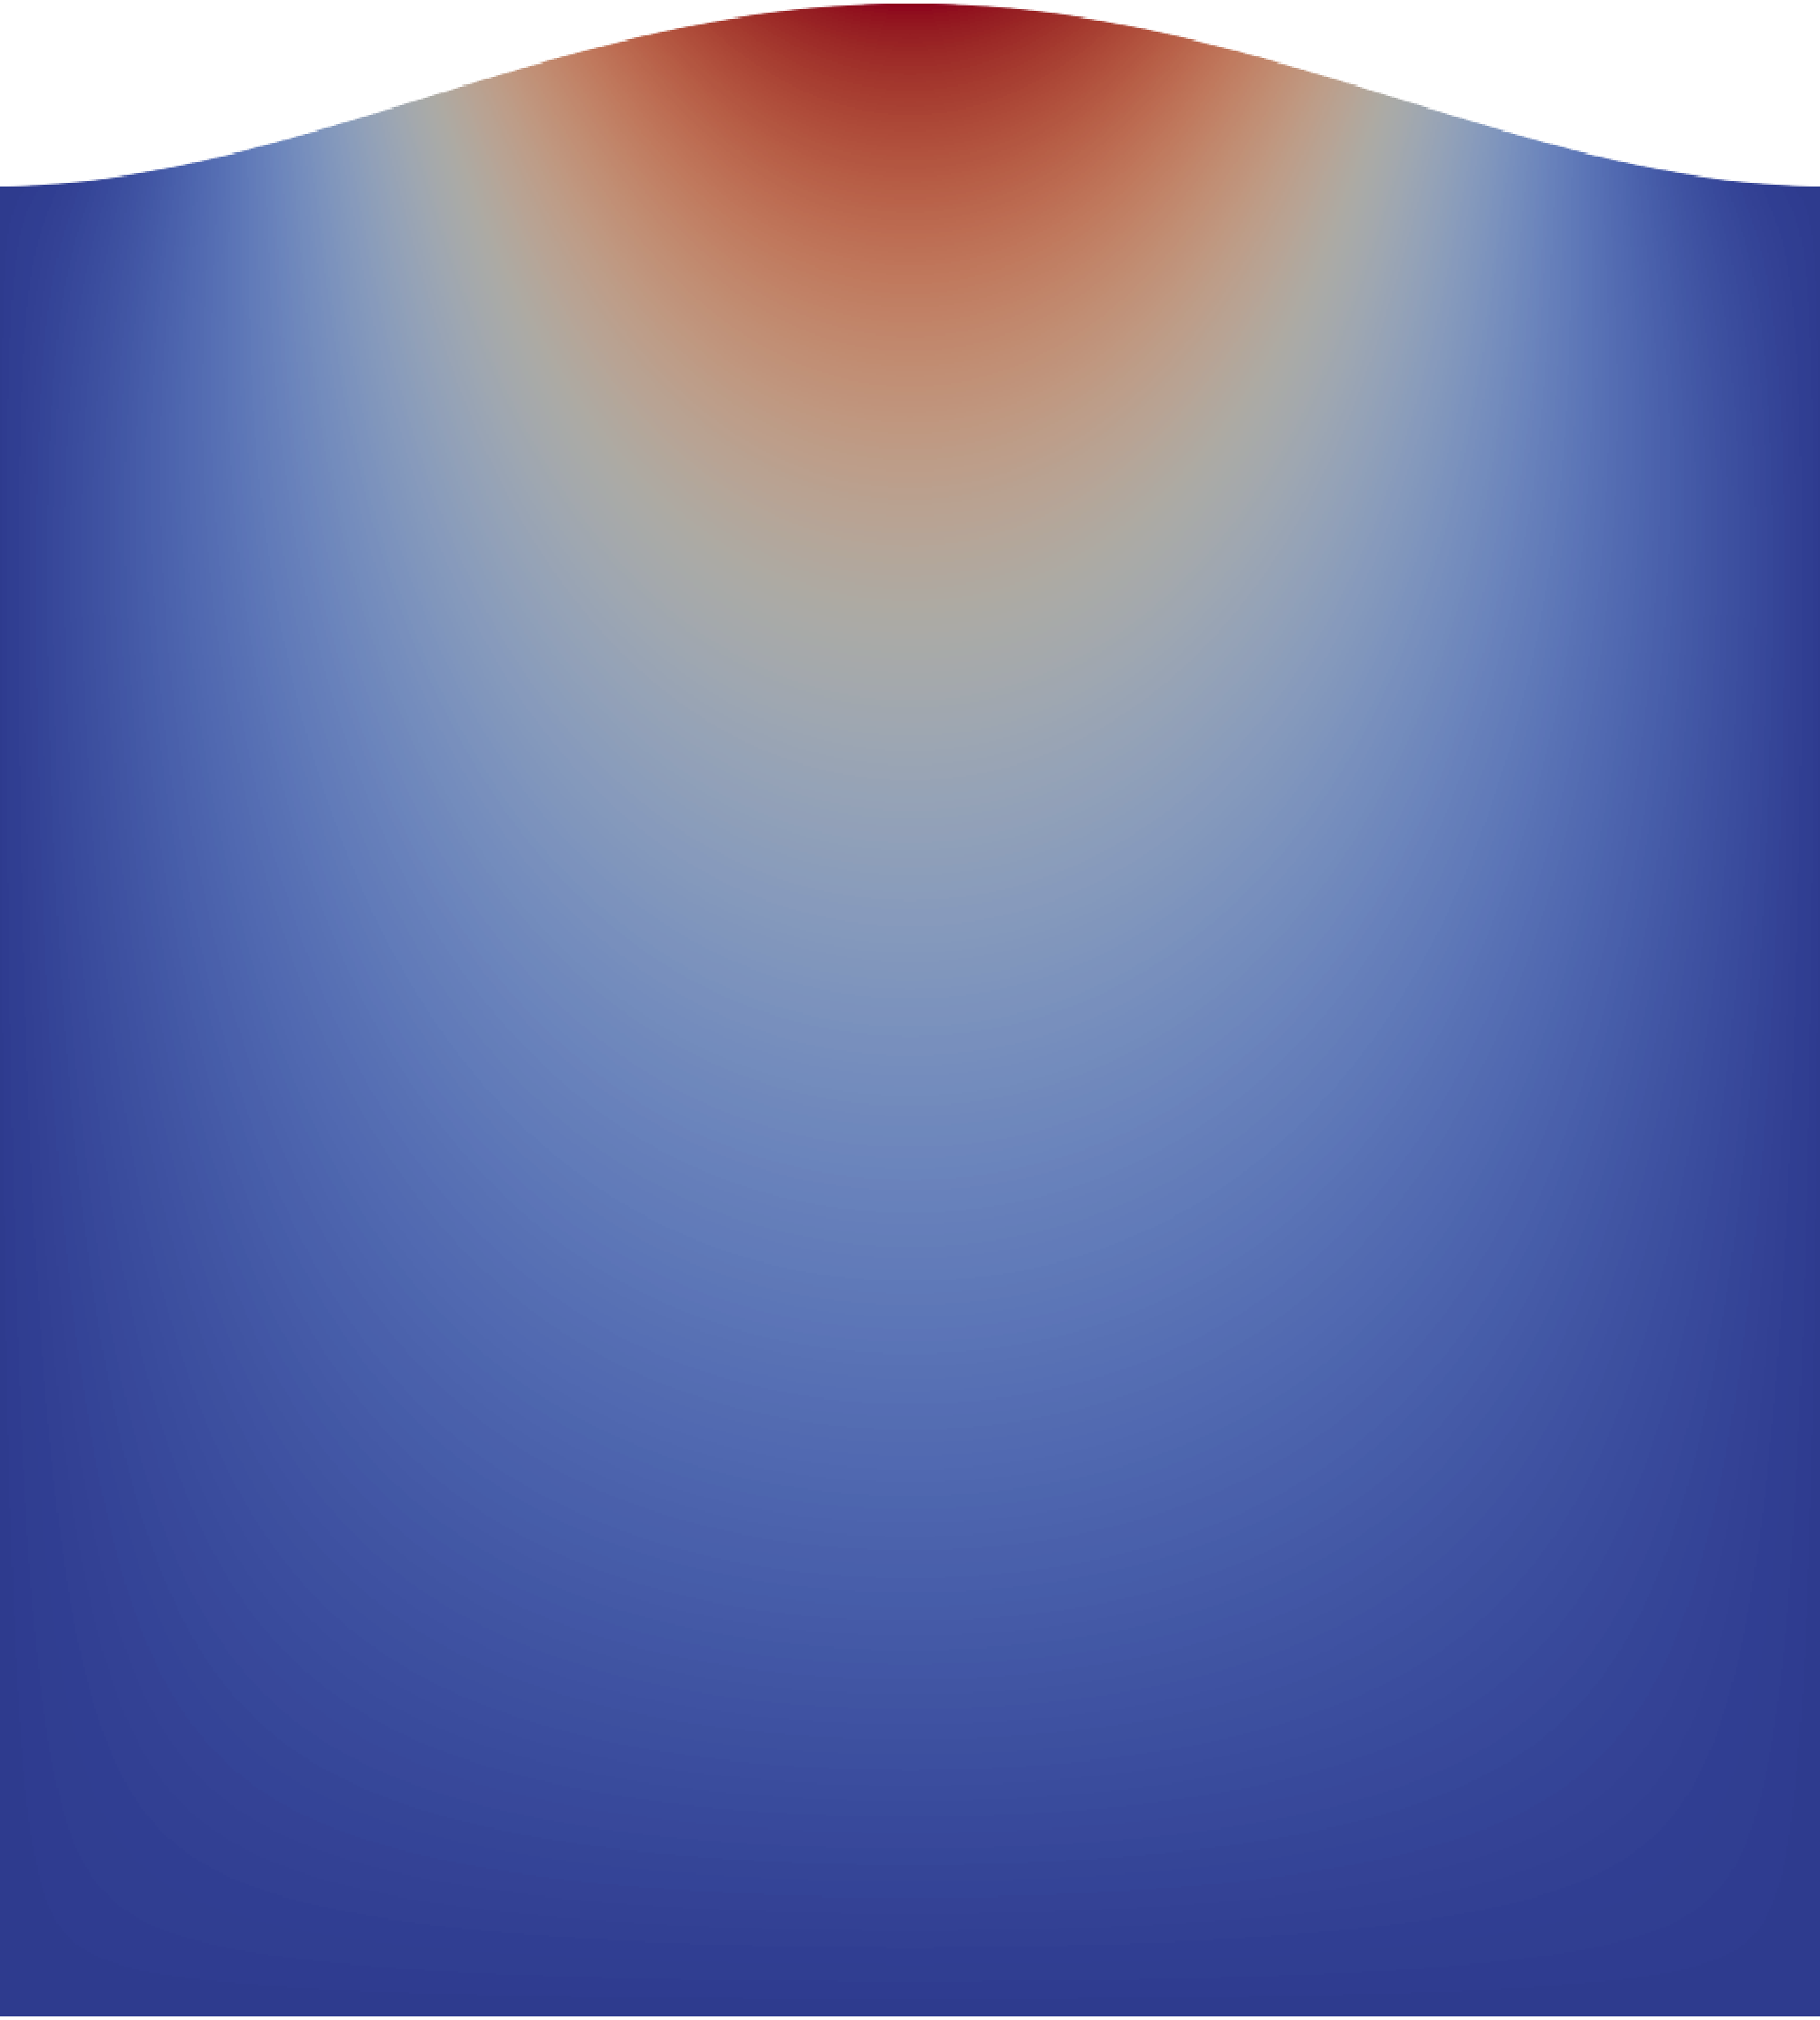
\includegraphics[width=0.5\textwidth]{figures/visualization-linear-elasticity1}
	\caption{Visualization of the considered linear elastic boundary value problem. A two-dimensional rectangular body undergoes an elastic deformation into y-direction.}
	\label{fig:visualization-linear-elasticity}
\end{figure}
We discretize equation \eqref{eq:linear-elasticity} with finite differences on a cartesian grid using a step size $h = 1/2^{l_{max}}$ with $l_{max} = 10$, which yields a system of linear equations $\boldsymbol{A} \boldsymbol{u} = \boldsymbol{f}$ with 
\begin{equation*}
	\boldsymbol{A} =
	\begin{pmatrix}
		(\alpha + \beta) \frac{\partial^2}{\partial x^2} + \alpha \nabla^2 & (\alpha + \beta) \frac{\partial^2}{\partial x \partial y} \\
		(\alpha + \beta) \frac{\partial^2}{\partial x \partial y} & (\alpha + \beta) \frac{\partial^2}{\partial y^2} +  \alpha \nabla^2
	\end{pmatrix},
\end{equation*}
\begin{equation*}
	\boldsymbol{u} = \begin{pmatrix}
		u \\ v
	\end{pmatrix}, \quad
	\boldsymbol{f} =
	\begin{pmatrix}
		f_{u} \\ f_{v}
	\end{pmatrix} =
	\begin{pmatrix}
		0 \\ 0
	\end{pmatrix},
\end{equation*}
whereby the differential operators $\nabla^2$, $\frac{\partial^2}{\partial x^2}$, $\frac{\partial^2}{\partial y^2}$ and $\frac{\partial^2}{\partial x \partial y}$ are approximated by their discrete counterparts
\begin{equation*}
	\left(\nabla^2 u\right)_{i,j} = 
	\frac{1}{h^2} \begin{bmatrix}
		0 & 1 & 0\\
		1 & -4 & 1 \\
		0 & 1 & 0  
	\end{bmatrix},
\end{equation*}
\begin{equation*}
	\left(\frac{\partial^2}{\partial x^2} u\right)_{i,j} =
		\frac{1}{h^2} \begin{bmatrix}
		0 & 0 & 0\\
		1 & -2 & 1 \\
		0 & 0 & 0  
	\end{bmatrix},
\end{equation*}
\begin{equation*}
	\left(\frac{\partial^2}{\partial y^2} u\right)_{i,j} =
	\frac{1}{h^2} \begin{bmatrix}
		0 & 1 & 0\\
		0 & -2 & 0 \\
		0 & 1 & 0  
	\end{bmatrix},
\end{equation*}
\begin{equation*}
	\left(\frac{\partial^2}{\partial x \partial y} u\right)_{i,j} = 
	\frac{1}{4 h^2} \begin{bmatrix}
		-1 & 0 & 1\\
		0 & 0 & 0 \\
		1 & 0 & -1  
	\end{bmatrix}.
\end{equation*}
Similar to the above case, we employ a uniform cartesian grid of size $h = 1/l_{max}$ with $l_{max} = 10$, such that the resulting system of linear equations contains $2\,093\,058$ unknowns.
\subsection{Multigrid Configuration}
\label{sec:experiments1-multigrid-configuration}
To design a multigrid method, we consider each of the given problems a grid hierarchy consisting of five discretization levels $l \in \left[l_{max} - 4, l_{max}\right]$, where the grid spacing on each level is given by the formula $h = 1/2^l$.
We then obtain the respective operator on each level by applying the same discretization method as described above.
Therefore, the resulting grammar is structurally similar to the one shown in Table~\ref{table:multigrid-grammar}.
Within each grammar production rule, we then consider the following components:
\begin{description}
	\item[\textbf{Smoothers}:] Decoupled / Collective Jacobi and red-black Gauss-Seidel, block Jacobi with rectangular blocks up to a maximum number of 6 terms.
	\item[\textbf{Restriction}:] Full-weighting restriction.
	\item[\textbf{Prolongation}:] Bilinear interpolation.
	\item[\textbf{Relaxation factors}:] $\omega \in \left( 0.1 + 0.05i \right)_{i = 0}^{36} = \left(0.1, 0.15, 0.2, \dots 1.9 \right)$
	\item[\textbf{Coarse-grid solver}:] Conjugate gradient method for $l = l_{max} - 4$.
\end{description}
Here, we generate block Jacobi smoothers by defining a splitting $A = L + D + U$ where $D$ is a block diagonal matrix of the form
\begin{equation*}
	D = 
		\begin{pmatrix}A_{11}&0&\cdots &0\\
			0&A_{22}&\cdots &0\\
			\vdots &\vdots &\ddots &\vdots \\0&0&\cdots &A_{mm}\end{pmatrix},
\end{equation*}
where each matrix $A_{ij}$ corresponds to a set of adjacent grid points contained in the respective rectangular block, as it has been discussed in Section~\ref{subsec:block-smoothing}.
A more detailed treatment of block relaxation methods can be found in~\cite{trottenberg2000multigrid}.
For each of smoothing and coarse-grid correction step the relaxation factor $\omega$ is chosen from the above sequence.
As a baseline for assessing the efficiency and generalizability of the evolved multigrid solvers, we consider a number of common multigrid cycles with red-black Gauss-Seidel smoothing and optimized relaxation factors.
We, therefore, formulate these methods on the same five-grid hierarchy, whereby we also utilize the same restriction, prolongation operators and coarse-grid solver, as described above.
In each case, we consider the corresponding linear system as solved when the initial residual has been reduced by a factor of $10^{-12}$.
\subsection{Optimization Settings and Evaluation Platform}
\label{sec:optimization-settings}
After specifying the operator and parameter choices considered within the construction of each multigrid solver, we next describe the settings under which we perform each GP-based optimization run.
Here, we utilize the EvoStencils framework, whose implementation has been described in detail in Chapter~\ref{chapter:evostencils-1} and~\ref{chapter:evostencils-2}.
The goal of each optimization run is then to evolve the set of non-dominated according to the two objectives convergence factor $\rho$ and execution time per iteration $t$, as described in Section~\ref{sec:fitness-evaluation-and-selection}, which are evaluated by applying each multigrid method as an iterative solver to the respective test problem.
The resulting individuals are then subject to a subsequent evaluation and comparison with the available reference methods. 
Table~\ref{table:gp-parameters} gives an overview about the configuration of the EvoStencils framework used within each experiment.
\begin{table}
	\centering
	\caption{Summary of GGGP configuration parameters.}
	\label{table:gp-parameters}
	\begin{tabular}{l c}
		\toprule
		Parameter & Value \\
		\midrule 
		Evolutionary algorithm type & $(\mu + \lambda)$ \\
		\midrule
		Objectives & $t, \rho$ \\
		\midrule
		Number of generations & 250 \\
		\midrule
		Initial population size & 2048 \\
		\midrule
		$\lambda$ & 256 \\
		\midrule
		$\mu$ & 256 \\
		\midrule
		Number of MPI processes & 64 \\
		\midrule
		Non-dominated sorting procedure & \cite{deb2002fast} \\ 
		\midrule
		Selection operator & \cite{deb2002fast} \\ 
		\midrule
		Crossover operator & Single-point crossover \\
		\midrule
		Crossover probability & $2/3$ \\
		\midrule
		Mutation operator & Random subtree replacement \\
		\midrule 
		Probability to mutate a terminal symbol & $1/3$ \\
		\bottomrule
	\end{tabular}
\end{table}
Within each run, starting with a randomly generated population of 2048 individuals, we perform an evolutionary search for 250 generations.
In each generation, we create new individuals by first selecting $\lambda = 256$ candidates from the current population.
We then apply mutation and crossover to each pair of selected candidates to create two child individuals, whereby the crossover probability is set to $2/3$ and in case of mutation we choose terminal symbol with a probability of $1/3$.
The resulting individuals are then evaluated according to the two objectives by generating a parallel C++ solver implementation using the ExaStencils framework, which is then applied to the respective problem as described above.
Hereby we distribute the evaluation of all 256 individuals to 64 MPI processes, such that each process is responsible for the evaluation of exactly four individuals.
The resulting fitness values are then distributed to all 64 processes, such that each of them possesses an identical copy of each child individual together with its fitness value, as it has been described in Chapter~\ref{sec:distributed-parallelization}.
Finally, we select $\mu = 256$ individuals as a population for the next generation from the combined set of parent and child individuals using the NSGA-II non-dominated sorting procedure~\cite{deb2002fast}.

As an evaluation platform for running each experiment, we employ 32 nodes of the Meggie compute cluster of the Erlangen National High Performance Computing Center (NHR), where each node of the system consists of two sockets, each with ten physical CPU cores.
Therefore, each process is pinned and executed on a dedicated socket, while for the evaluation of each solver we employ a thread-based parallelization using ten OpenMP threads, where each tread is pinned to a distinct physical compute core on the respective socket.
For the parallelization of each nested loop, we employ a static scheduling based on the outer loop, such that each threads processes a consecutive chunk of iterations.
To generate a thread-parallel executable for each solver, we employ GCC 9.3.0 with the -O3 optimization level.
Finally, we execute each solver three times and then compute the average for both objectives to reduce statistical variations between individual evaluation runs.

\subsection{Algorithm Behavior Analysis}
As a first step towards a quantitative evaluation of our evolutionary search method, we assess whether our algorithm is able to effectively find good solutions with respect to our two optimization objectives.
For this purpose, we measure the minimum of each of the two objectives within the population throughout each of the ten optimization runs for all three test problems.
As a result, Figure~\ref{fig:poisson-2D-minimum-objectives},~\ref{fig:poisson-3D-minimum-objectives} and~\ref{fig:linear-elasticity-2D-minimum-objectives} shows the mean and standard deviation of the current optimum of both objectives over each of the ten optimization runs.
\begin{figure}
	\centering
	\begin{subfigure}[b]{0.49\textwidth}
		\centering
		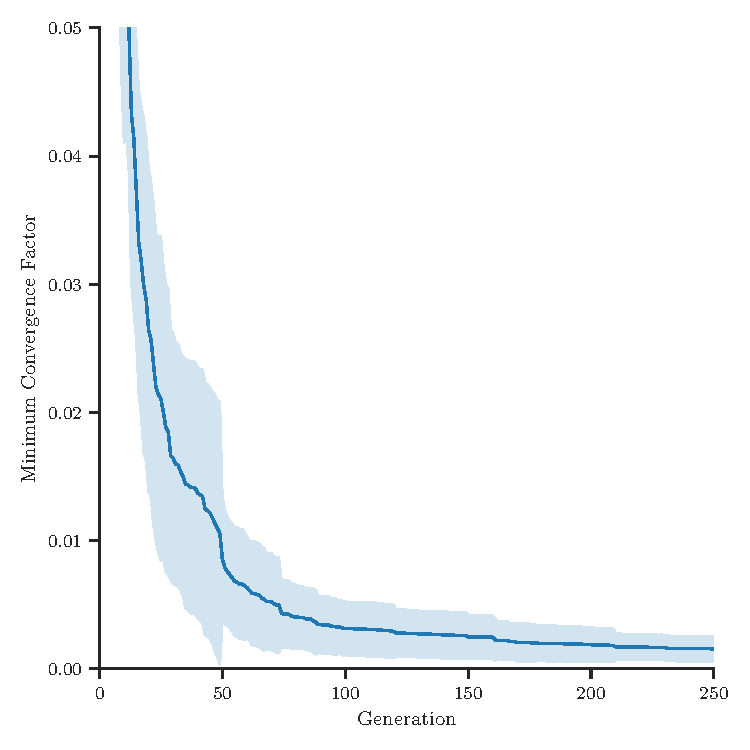
\includegraphics[width=\textwidth]{figures/minimum_convergence_factor_2D_FD_Poisson_fromL2.pdf}
		\caption{Minimum Convergence Factor}
		\label{fig:poisson-2D-minimum-convergence-factor}
	\end{subfigure}
	\hfill
	\begin{subfigure}[b]{0.49\textwidth}
		\centering
		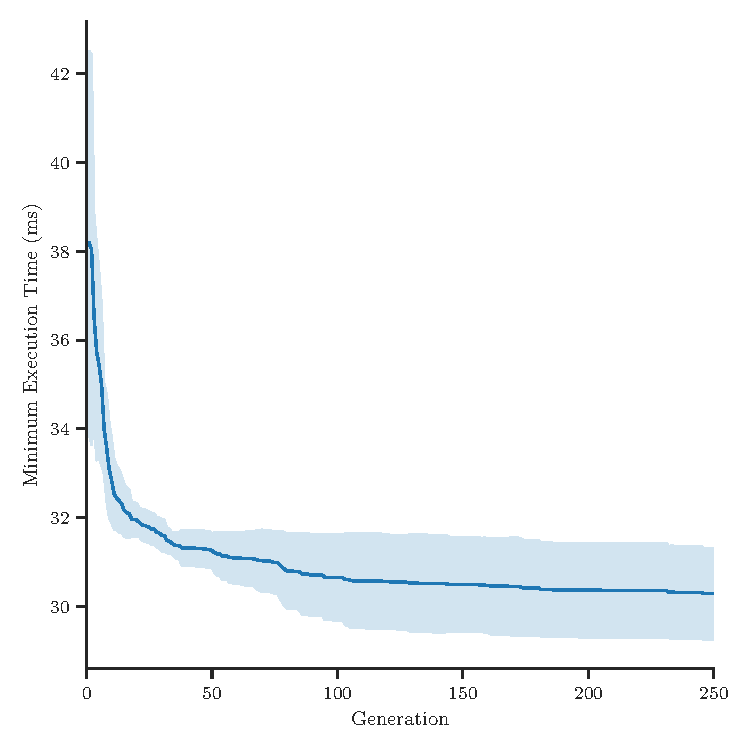
\includegraphics[width=\textwidth]{figures/minimum_execution_time_2D_FD_Poisson_fromL2.pdf}
		\caption{Minimum Execution Time per Iteration}
		\label{fig:poisson-2D-minimum-execution-time}
	\end{subfigure}
	\caption{2D Poisson - Mean and standard deviation of the minimum objective function values during the optimization.}
	\label{fig:poisson-2D-minimum-objectives}
\end{figure}
\begin{figure}
	\centering
	\begin{subfigure}[b]{0.49\textwidth}
		\centering
		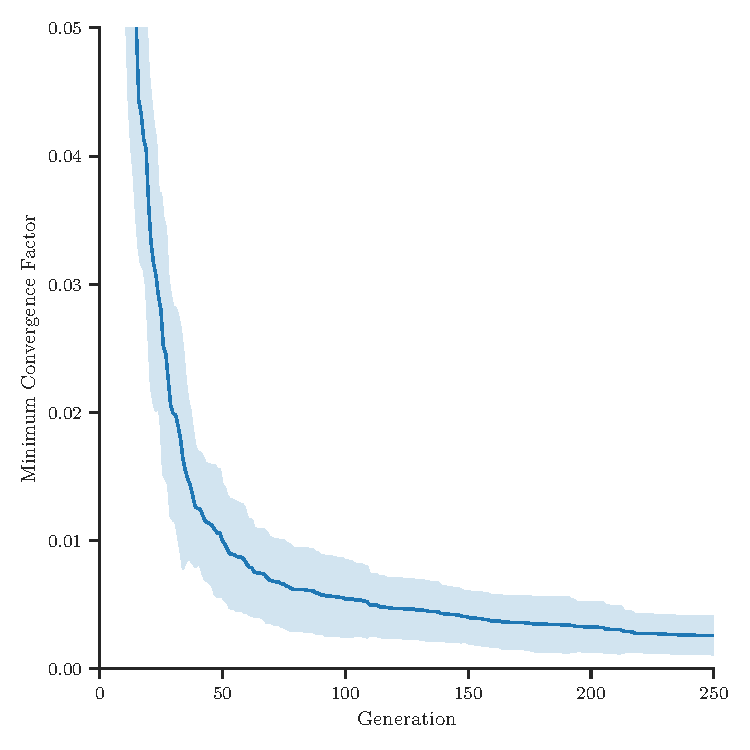
\includegraphics[width=\textwidth]{figures/minimum_convergence_factor_3D_FD_Poisson_fromL2.pdf}
		\caption{Minimum Convergence Factor}
		\label{fig:poisson-3D-minimum-convergence-factor}
	\end{subfigure}
	\hfill
	\begin{subfigure}[b]{0.49\textwidth}
		\centering
		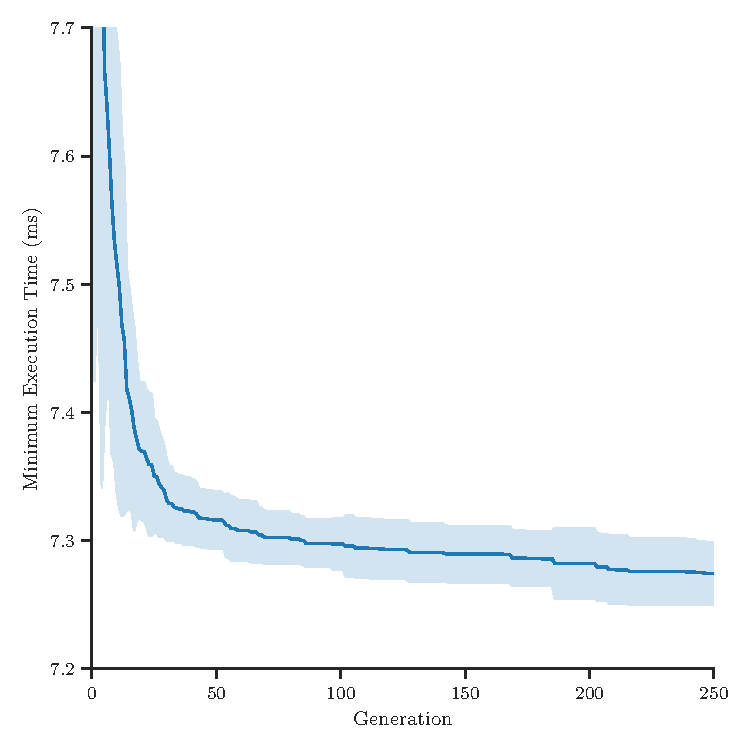
\includegraphics[width=\textwidth]{figures/minimum_execution_time_3D_FD_Poisson_fromL2.pdf}
		\caption{Minimum Execution Time per Iteration}
		\label{fig:poisson-3D-minimum-execution-time}
	\end{subfigure}
	\caption{3D Poisson - Mean and standard deviation of the minimum objective function values during the optimization.}
	\label{fig:poisson-3D-minimum-objectives}
\end{figure}
\begin{figure}
	\centering
	\begin{subfigure}[b]{0.49\textwidth}
		\centering
		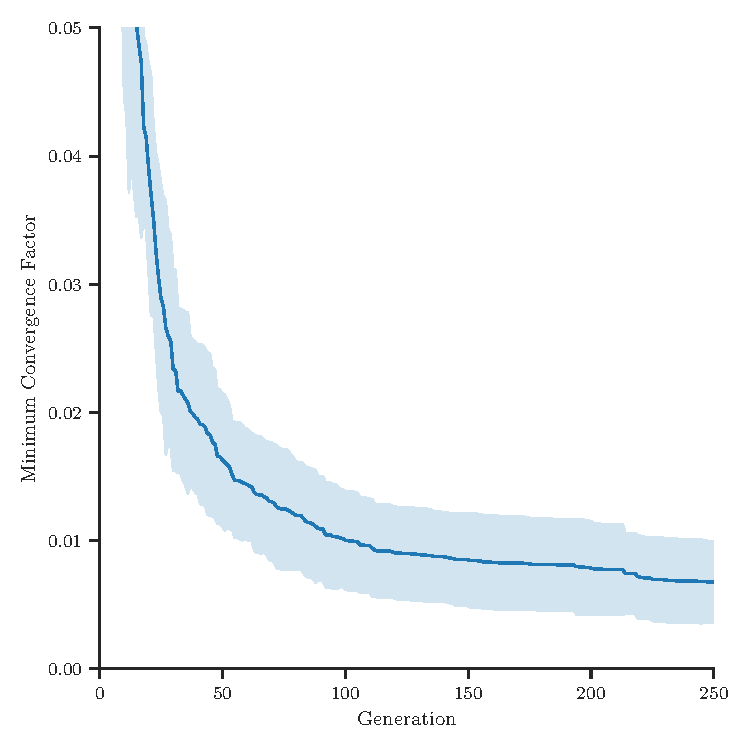
\includegraphics[width=\textwidth]{figures/minimum_convergence_factor_2D_FD_LinearElasticity_fromL2.pdf}
		\caption{Minimum Convergence Factor}
		\label{fig:linear-elasticity-2D-minimum-convergence-factor}
	\end{subfigure}
	\hfill
	\begin{subfigure}[b]{0.49\textwidth}
		\centering
		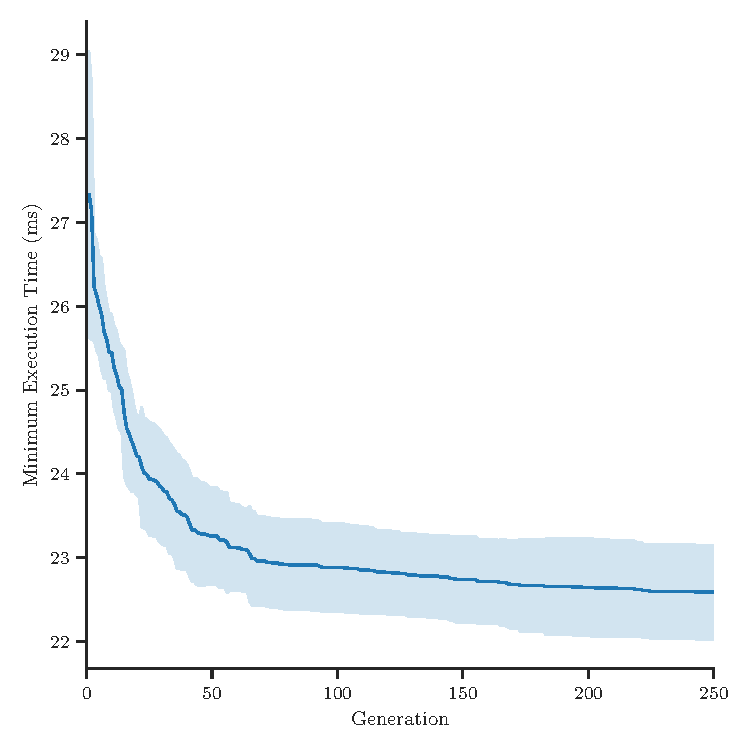
\includegraphics[width=\textwidth]{figures/minimum_execution_time_2D_FD_LinearElasticity_fromL2.pdf}
		\caption{Minimum Execution Time per Iteration}
		\label{fig:linear-elasticity-2D-minimum-execution-time}
	\end{subfigure}
	\caption{2D Linear Elasticity - Mean and standard deviation of the minimum objective function values during the optimization.}
	\label{fig:linear-elasticity-2D-minimum-objectives}
\end{figure}
First of all, in general we can assess that in all three cases our algorithm is able to quickly reduce the minimum value of both objectives within the population.
However, if we compare the slope of the two objectives for the three different problems, we can see that in case of the first objective $\rho$ significantly more generations are required to achieve the same degree of reduction as for the second objective $t$.
In all three cases, the algorithm still significantly improves upon the current minimum of $\rho$ beyond the first 50 generations, which can be seen in Figure~\ref{fig:poisson-2D-minimum-convergence-factor},~\ref{fig:poisson-3D-minimum-convergence-factor} and~\ref{fig:linear-elasticity-2D-minimum-convergence-factor}.
In contrast, for the second objective $t$, the majority of improvement happens within the first 50--70 generations, as it can be seen in Figure~\ref{fig:poisson-2D-minimum-execution-time},~\ref{fig:poisson-3D-minimum-execution-time} and~\ref{fig:linear-elasticity-2D-minimum-execution-time}.
At this point it is also important to consider that while the convergence factor is constant for each execution of the same solver, $t$ is obtained by measuring its execution time on the respective compute node.
Therefore, due to manufacturing and temperature-based variations, we can expect a certain degree of fluctuations when measuring the execution time of the same solver on different compute nodes during consecutive optimization runs.
Consequently, even though the algorithm is more effective in quickly reducing the second objective, this results in a larger deviations between individual optimizations runs and, thus, a overall higher standard deviation.

Second, by considering the absolute value of the minimum convergence factor attained in each of the three different cases, we can assess the difficulty of the underlying problem.
While the execution time per iteration, as a second objective, is solely determined by the computational complexity of each solver and the properties of the given computer architecture it is executed on, a smaller convergence factor indicates that the underlying problem is easier to solve.
Poisson's equation represents an often-studied model problem, whose strong ellipticity enables its effective solution using multigrid methods~\cite{trottenberg2000multigrid}.
As a consequence, our algorithm is able to consistently evolve multigrid methods that achieve fast convergence, with minimum convergence factors of less than 0.005, in solving both the two and three dimensional instances of this equation, which can be seen in Figure~\ref{fig:poisson-2D-minimum-convergence-factor} and~\ref{fig:poisson-3D-minimum-convergence-factor}.
In case of the linear elastic boundary value problem, both the mean and standard deviation remain higher for the first objective throughout the optimization.
However, on average our algorithm is still able to evolve multigrid methods that achieve a convergence factor of 0.01 of less and, therefore, outstandingly fast convergence.
In summary, we can conclude that our search method is able to consistently find satisfactory minima for both objectives in all three test cases considered.

To further analyze the behavior of our multi-objective evolutionary algorithm, we consider the distribution of non-dominated individuals at the end of all optimization runs, which is shown in Figure~\ref{fig:pareto-front-2D-poisson},~\ref{fig:pareto-front-3D-poisson} and~\ref{fig:pareto-front-2D-linear-elasticity}.
\begin{figure}
	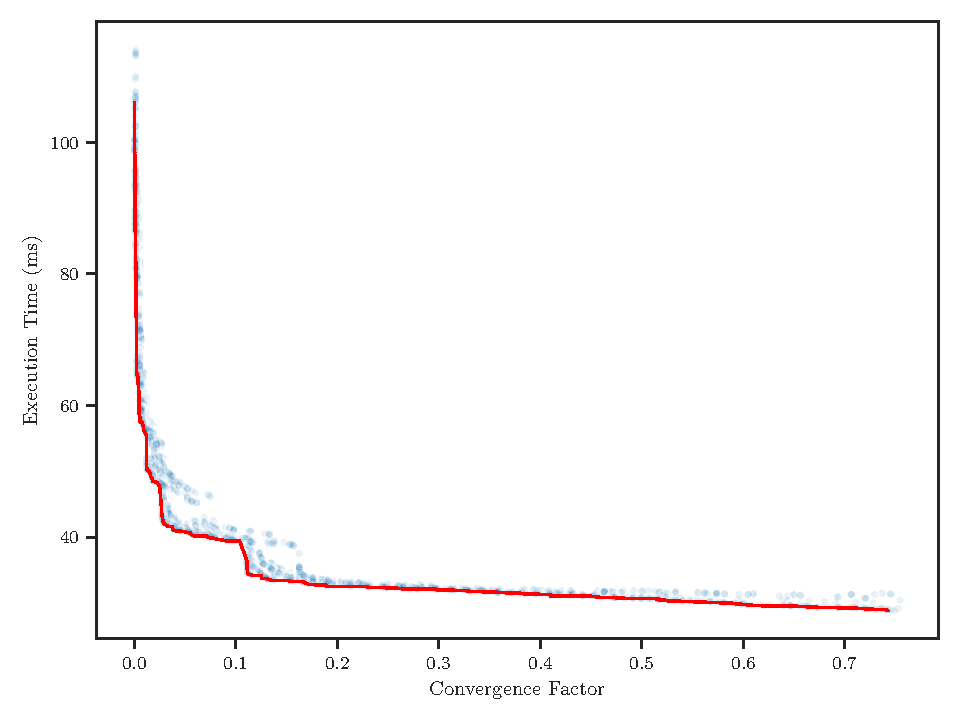
\includegraphics[width=\columnwidth]{figures/pareto_front_2D_FD_Poisson_fromL2.pdf}
	\caption{2D Poisson - Distribution of non-dominated individuals at the end of all ten experiments. The red line denotes the combined Pareto front.}
	\label{fig:pareto-front-2D-poisson}
\end{figure}
\begin{figure}
	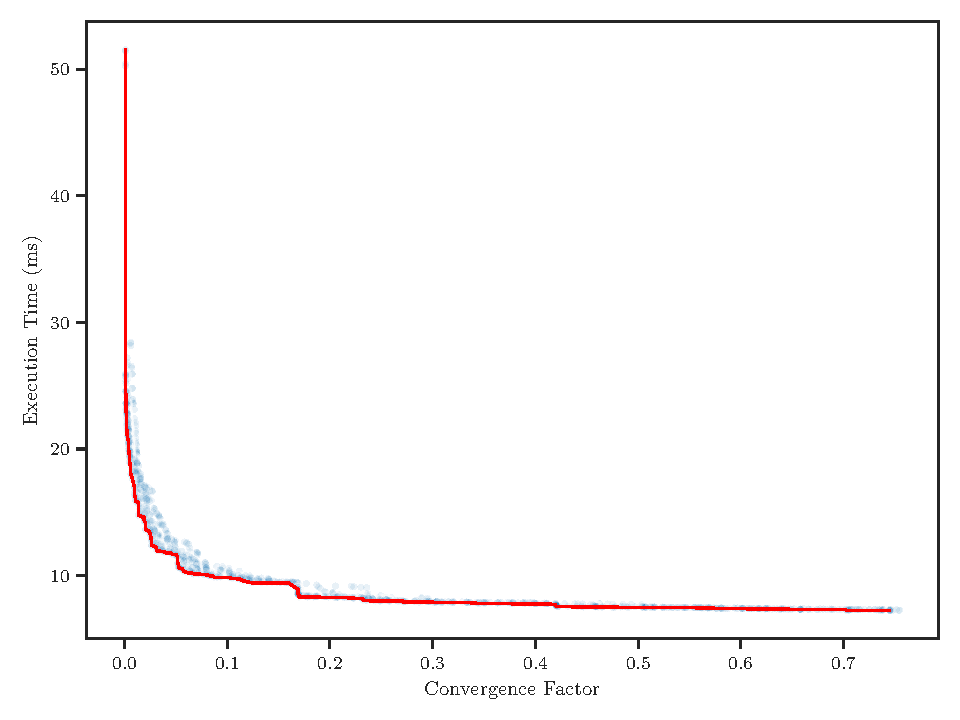
\includegraphics[width=\columnwidth]{figures/pareto_front_3D_FD_Poisson_fromL2.pdf}
	\caption{3D Poisson - Distribution of non-dominated individuals at the end of all ten experiments. The red line denotes the combined Pareto front.}
	\label{fig:pareto-front-3D-poisson}
\end{figure}
\begin{figure}
	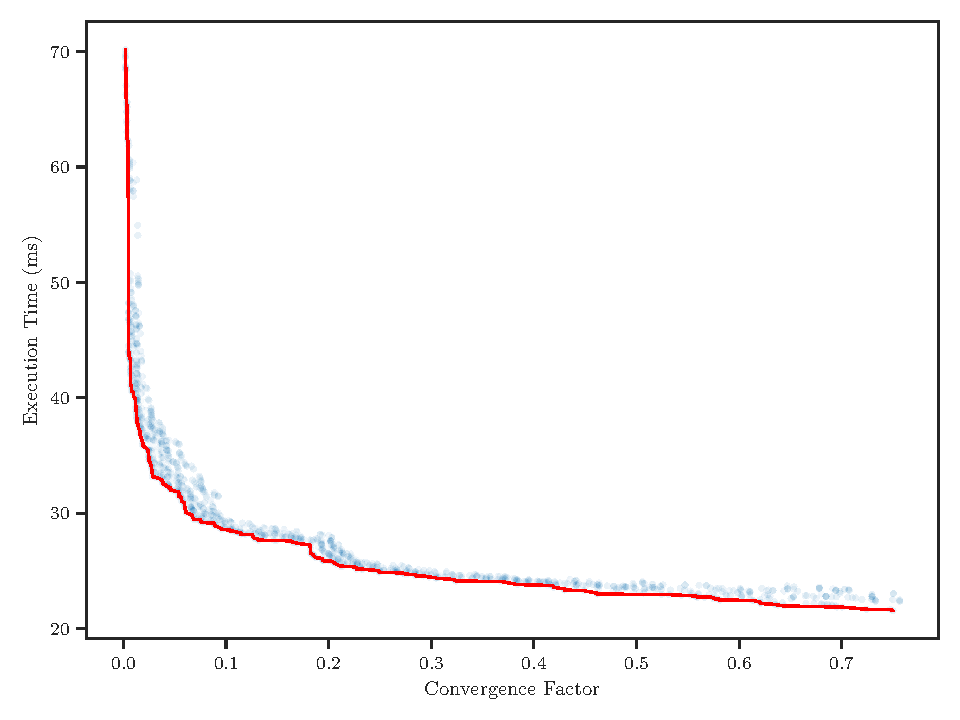
\includegraphics[width=\columnwidth]{figures/pareto_front_2D_FD_LinearElasticity_fromL2.pdf}
	\caption{2D Linear Elasticity - Distribution of non-dominated individuals at the end of all ten experiments. The red line denotes the combined Pareto front.}
	\label{fig:pareto-front-2D-linear-elasticity}
\end{figure}
Here the red line denotes the combined front while the color density of the distribution indicates where the majority of solutions is located at the end of all experiments. 
In all three cases, the majority of non-dominated solutions evolved within each experiment can be found close to the combined front.
While in Figure~\ref{fig:pareto-front-2D-poisson} the number of solutions that are distinctly located outside of the front is slightly higher than in the other two cases, their distance to the next point on this front is still comparably small compared to the complete objective space.
Again we can attribute part of this effect to measurement variations in the solver execution time on different compute nodes.
Furthermore, note that for the most part and especially the center of the objective space, the solutions are evenly distributed alongside the front.
Here only the left-upper part of Figure~\ref{fig:pareto-front-3D-poisson} and~\ref{fig:pareto-front-2D-linear-elasticity} represents a noteworthy exception, where the algorithm struggles to find the same solutions within each run.
This effect can be mainly attributed to the fact that the solutions located at this part of the space are characterized by an extremely fast convergence.
Since the convergence of a multigrid method can be first and foremost accelerated with the addition of smoothing and coarse-grid correction steps, finding the same non-dominated solutions with fast convergence requires us to evolve increasingly large expression of the same structure in individual experiments.
Recently, the limited capabilities of NSGA-II to evolve large non-dominated expressions have been demonstrated in~\cite{liu2022evolvability}, which, therefore, similarly offers an explanation for the impaired evolution of fast-converging solutions in the given case.
\subsection{Comparison with Reference Methods}
Finally, in order to investigate whether our approach yields multigrid methods that are competitive with well-known multigrid cycles, we consider two different recent multi-core CPU architectures for evaluation: Intel Xeon E5-2630v4 (Broadwell) and Intel Xeon 2660v2 (Ivy Bridge).
In both cases, each compute node consists of two sockets with 20 physical CPU cores and a cache-coherent NUMA architecture.
Each solver is then executed on a dedicated node using a thread-based parallelization with 20 OpenMP threads, whereby we pin each thread to a unique physical core and employ the same parallelization approach as described in Section~\ref{sec:optimization-settings}.
In order to assess the solving speed of the methods evolved, we consider two different problem sizes for each of the three test cases.
While in the first case a problem size identical to the one employed within the optimization is chosen, in the second case we obtain a larger one by doubling number of grid points in each dimension.
Even though the evaluation of our methods generalizability is not the focus of this section, it is still worthwhile to investigate whether the methods evolved with our approach also are capable of solving larger instances of the same problem.
For comparison we consider a number of different V-cycles with at most four red-black Gauss-Seidel pre and post-smoothing steps, as these methods are known to lead to the fastest multigrid-based solvers for Poisson's equation according to the classical formulation of multigrid shown in Algorithm~\ref{alg:multigrid-cycle}~\cite{trottenberg2000multigrid}.
As we have already investigated in~\cite{schmitt2020constructing}, the same is true for the linear elastic boundary value problem considered here.
To achieve a fair comparison, we empirically choose the optimum relaxation factor $\omega$ for each test case from the same interval considered within the optimization, which leads to $\omega = 1.15$ for the two-dimensional Poisson equation and $\omega = 1.25$ both for the three-dimensional Poisson equation and the linear elastic boundary value problem.
Table~\ref{table:poisson-2D-reference-methods},~\ref{table:poisson-3D-reference-methods} and~\ref{table:linear-elasticity-2D-reference-methods} contains the resulting solving times and number of iterations to achieve the required defect reduction for the respective test case.
Here, for instance, the abbreviation V(2, 1) denotes a V-cycle with two pre and one post-smoothing step with red-black Gauss-Seidel.
First of all, as we can expect from a functioning multigrid method, the number of iterations stays constant for both problem sizes, only with the exception of the V(1,0)-cycle, where we can observe a slight increase for the linear elastic boundary value problem.
Overall, we can conclude that while the V(2,2)-cycle represents the fastest solver for both cases of Poisson's equation, the V(3,3) cycle leads to the fastest solving time in case of the linear elastic boundary value problem.
\begin{table}
	\caption{2D Poisson - Measured number of iterations and solving times of the reference methods on 20 cores and two sockets.}
	\label{table:poisson-2D-reference-methods}
	\centering
	\begin{tabular}{l c c c c c c}
		\toprule
		& \multicolumn{2}{c}{Iterations} & \multicolumn{2}{c}{Broadwell (ms)} & \multicolumn{2}{c}{Ivy Bridge (ms)} \\
		\cmidrule(r){2-3} \cmidrule(r){4-5} \cmidrule(r){6-7}
		$l_{max}$ & $11$& $12$ & $11$ & $12$ & $11$ & $12$\\
		\midrule
		V(1, 0) & 21 & 21 & 969 & 2810 & 879 & 2652 \\
		\midrule
		V(1, 1) & 9 & 9 & 461 & 1359 & 411 & 1287 \\
		\midrule
		V(2, 1) & 7 & 7 & 377 & 1137 & 334 & 1087\\
		\midrule
		V(2, 2) & 6 & 6 & 344 & 1056 & 302 & 1007 \\
		\midrule
		V(3, 2) & 6 & 6 & 378 & 1160 & 324 & 1112 \\
		\midrule
		V(3, 3) & 6 & 6 & 397 & 1255 & 344 & 1201 \\
		\midrule
		V(4, 3) & 6 & 6 & 425 & 1350 & 366 & 1306 \\
		\midrule
		V(4, 4) & 6 & 6 & 448 & 1449 & 383 & 1409\\
		\bottomrule
	\end{tabular}
	%FMG for max_level = 12: 530.3038500000001 ms, 3 Iterations
\end{table}
\begin{table}
	\caption{3D Poisson - Measured number of iterations and solving times of the reference methods on 20 cores and two sockets.}
	\label{table:poisson-3D-reference-methods}
	\centering
	\begin{tabular}{l c c c c c c}
		\toprule
		& \multicolumn{2}{c}{Iterations} & \multicolumn{2}{c}{Broadwell (ms)} & \multicolumn{2}{c}{Ivy Bridge (ms)} \\
		\cmidrule(r){2-3} \cmidrule(r){4-5} \cmidrule(r){6-7}
		$l_{max}$ & $7$& $8$ & $7$ & $8$ & $7$ & $8$\\
		\midrule
		V(1, 0) & 29 & 30 & 121.3 &1221 & 134.6 & 1470 \\
		\midrule
		V(1, 1) & 13 & 13 & 70.8 & 682 & 79.9 & 838 \\
		\midrule
		V(2, 1) & 9 & 9 & 59.0 & 582 & 66.2 & 708 \\
		\midrule
		V(2, 2) & 7 & 7 & 54.6 & 531 & 65.4 & 654 \\
		\midrule
		V(3, 2) & 7 & 7 & 61.9 & 610 & 74.6 & 757 \\
		\midrule
		V(3, 3) & 7 & 7 & 72.6 & 690 & 86.6 & 857 \\
		\midrule
		V(4, 3) & 7 & 6 & 77.9 & 656 & 87.3 & 825 \\
		\midrule
		V(4, 4) & 6 & 6 & 73.2 & 725 & 82.5 & 906 \\
		\bottomrule
	\end{tabular}
\end{table}
\begin{table}
	\caption{2D Linear Elasticity - Measured number of iterations and solving times of the reference methods on 20 cores and two sockets.}
	\label{table:linear-elasticity-2D-reference-methods}
	\centering
	\begin{tabular}{l c c c c c c}
		\toprule
		& \multicolumn{2}{c}{Iterations} & \multicolumn{2}{c}{Broadwell (ms)} & \multicolumn{2}{c}{Ivy Bridge (ms)} \\
		\cmidrule(r){2-3} \cmidrule(r){4-5} \cmidrule(r){6-7}
		$l_{max}$ & $10$& $11$ & $10$ & $11$ & $10$ & $11$\\
		\midrule
		V(1, 0) & 32 & 31 & 872 & 4306 & 828 & 4128 \\
		\midrule
		V(1, 1) & 15 & 15 & 439 & 2118 & 418 & 2075\\
		\midrule
		V(2, 1) & 10 & 10 & 318 & 1529 & 312 & 1529 \\
		\midrule
		V(2, 2) & 9 & 9 & 314 & 1449 & 316 & 1476 \\
		\midrule
		V(3, 2) & 8 & 8 & 297 & 1368 & 304 & 1388 \\
		\midrule
		V(3, 3) & 7 & 7 & 283 & 1247 & 288 & 1288 \\
		\midrule
		V(4, 3) & 7 & 7 & 293 & 1320 & 313 & 1397 \\
		\midrule
		V(4, 4) & 7 & 7 & 311 & 1378 & 334 & 1471 \\
		\bottomrule
	\end{tabular}
\end{table}

Finally, we can then evaluate the multigrid methods obtained with our grammar-guided search method in each of the ten experiments under the same conditions.
As the number of non-dominated individuals within the population at the end of each run is unrestricted and can, therefore, be too high for a direct evaluation, we heuristically identify the 50 most promising individuals by sorting them according to the metric
\begin{equation}
	T_{\varepsilon} = \frac{\log(\varepsilon)}{\log(\rho)} \cdot t,
\end{equation}
where $\varepsilon = 10^{-12}$ is the desired defect reduction factor and $\rho$ and $t$ the objective function values obtained within the optimization.
Each of the resulting methods is then executed as a solver for the respective test problem on a Broadwell compute node consisting of two sockets with 20 CPU cores, whereby we employ the same problem size as within the optimization.
Note that while the problem size and computer architecture is identical to the one used within the optimization, increasing the number of CPU cores leads to a higher degree of parallelism and, thus, smaller execution time per iteration, which necessitates the reevaluation of each method.
After we have identified the method that leads to the fastest solver in each experiment, we execute it on both problem sizes and evaluation platforms, as described above.
Table~\ref{table:poisson-2D-evolved-methods},~\ref{table:poisson-3D-evolved-methods} and~\ref{table:linear-elasticity-2D-evolved-methods} contain the resulting measured solving times for each case.
\begin{table}
	\caption{2D Poisson - Measured number of iterations and solving times of the evolved multigrid methods on 20 cores and two sockets.}
	\label{table:poisson-2D-evolved-methods}
	\centering
	\begin{tabular}{l c c c c c c}
		\toprule
		& \multicolumn{2}{c}{Iterations} & \multicolumn{2}{c}{Broadwell (ms)} & \multicolumn{2}{c}{Ivy Bridge (ms)} \\
		\cmidrule(r){2-3} \cmidrule(r){4-5} \cmidrule(r){6-7}
		$l_{max}$ & $11$& $12$ & $11$ & $12$ & $11$ & $12$\\
		\midrule
		ES-1 & 5 & 5 & 338 & 1064 & 304 & 1055\\
		\midrule
		ES-2 & 6 & 6 & 371 & 1163 & 330 & 1133 \\
		\midrule
		ES-3 & 5 & 5 & 311 & 988 & 279 & 976 \\
		\midrule
		ES-4 & 6 & 6 & 380 & 1188 & 338 & 1153 \\
		\midrule
		ES-5 & 5 & 5 & 312 & 978 & 279 & 963 \\
		\midrule
		ES-6 & 5 & 5 & 349 & 1123 & 309 & 1106 \\
		\midrule
		ES-7 & 6 & 6 & 354 & 1096 & 320 & 1068 \\
		\midrule
		ES-8 & 6 & 6 & 347 & 1081 & 310 & 1056 \\
		\midrule
		ES-9 & 6 & 6 & 353 & 1079 & 313 & 1045 \\
		\midrule
		ES-10 & 5 & 5 & 310 & 960 & 275 & 934 \\
		\bottomrule
	\end{tabular}
\end{table}
\begin{table}
	\caption{3D Poisson - Measured number of iterations and solving times of the evolved multigrid methods on 20 cores and two sockets.}
	\label{table:poisson-3D-evolved-methods}
	\centering
	\begin{tabular}{l c c c c c c}
		\toprule
		& \multicolumn{2}{c}{Iterations} & \multicolumn{2}{c}{Broadwell (ms)} & \multicolumn{2}{c}{Ivy Bridge (ms)} \\
		\cmidrule(r){2-3} \cmidrule(r){4-5} \cmidrule(r){6-7}
		$l_{max}$ & $7$& $8$ & $7$ & $8$ & $7$ & $8$\\
		\midrule
		ES-1 & 10 & 11 & 55.3 & 577 & 70.0 & 704\\
		\midrule
		ES-2 & 8 & 9 & 57.2 & 578 & 64.3 & 716 \\
		\midrule
		ES-3 & 8 & 9 & 59.0 & 671 & 65.3 & 824 \\
		\midrule
		ES-4 & 8 & 9 & 54.6 & 576 & 62.7 & 710 \\
		\midrule
		ES-5 & 8 & 10 & 54.6 & 641 & 60.9 & 789 \\
		\midrule
		ES-6 & 9 & 10 & 59.4 & 716 & 67.1 & 891 \\
		\midrule
		ES-7 & 6 & 8 & 56.2 & 702 & 70.9 & 880 \\
		\midrule
		ES-8 & 5 & 5 & 56.7 & 589 & 74.0 & 724 \\
		\midrule
		ES-9 & 10 & 10 & 61.0 & 568 & 66.3 & 681 \\
		\midrule
		ES-10 & 10 & 11 & 55.4 & 581 & 61.3 & 705 \\
		\bottomrule
	\end{tabular}
\end{table}
\begin{table}
	\caption{2D Linear Elasticity - Measured number of iterations and solving times of the evolved multigrid methods on 20 cores and two sockets.}
	\label{table:linear-elasticity-2D-evolved-methods}
	\centering
	\begin{tabular}{l c c c c c c}
		\toprule
		& \multicolumn{2}{c}{Iterations} & \multicolumn{2}{c}{Broadwell (ms)} & \multicolumn{2}{c}{Ivy Bridge (ms)} \\
		\cmidrule(r){2-3} \cmidrule(r){4-5} \cmidrule(r){6-7}
		$l_{max}$ & $10$& $11$ & $10$ & $11$ & $10$ & $11$\\
		\midrule
		ES-1 & 6 & 6 & 234 & 1117 & 235 & 1137 \\
		\midrule
		ES-2 & 6 & 6 & 216 & 1033 & 211 & 1035 \\
		\midrule
		ES-3 & 7 & 7 & 258 & 1225 & 259 & 1231 \\
		\midrule
		ES-4 & 6 & 6 & 226 & 1077 & 219 & 1093 \\
		\midrule
		ES-5 & 6 & 6 & 235 & 1121 & 229 & 1139 \\
		\midrule
		ES-6 & 6 & 6 & 220 & 1083 & 213 & 1093 \\
		\midrule
		ES-7 & 7 & 7 & 238 & 1191 & 236 & 1186 \\
		\midrule
		ES-8 & 6 & 6 & 217 & 1037 & 223 & 1039 \\
		\midrule
		ES-9 & 6 & 6 & 224 & 1039 & 222 & 1058 \\
		\midrule
		ES-10 & 7 & 7 & 243 & 1188 & 238 & 1188 \\
		\bottomrule
	\end{tabular}
\end{table}
In general, we can conclude that in all three cases our evolutionary search method was able to consistently find well-functioning multigrid methods, which lead to fast solving times for both problem sizes in each of the three cases considered.
Furthermore, in case of the two-dimensional Poisson equation and linear elasticity our method is able to discover multigrid methods that achieve an even higher degree of efficiency in reducing a given error than the best known reference cycle.
Here, the fastest evolved method for the two-dimensional Poisson equation, ES-10, leads to a $9 \%$ solving time improvement compared to the V(2,2)-cycle on both architectures, while for linear elasticity the ES-2 method achieves an even larger speedup of 17--27 \% compared to the V(3,3)-cycle.
Interestingly, in contrast to the other two cases, for the two-dimensional Poisson equation all solvers achieve faster execution times on the older Ivy Bridge computer architecture.
However, further investigating this phenomenon would require us to perform an in depth analysis of the generated code, which is out of the scope of this work as our focus is a comparison of the relative performance of different multigrid methods on the same architecture.
While in case of the three-dimensional Poisson, the methods evolved with our approach are all able to achieve competitive solving times, compared to the other two cases, not the same degree of efficiency can be achieved for both problem sizes.
In particular, with the exception of the evolved methods ES-8 and ES9, we observe a slight increase in the number of iterations for the larger instance of this problem, which leads to a stronger increase of the solving times compared to the reference method.
This effect indicates that not all multigrid methods evolved for a particular instance of this test problem can be generalized to larger problem instances without further adaption.
In Section~\ref{sec:generalization}, we have already addressed this problem by proposing a multigrid-specific generalization scheme, whose effectiveness will be investigated in the next section of this chapter.   
%we have already presented an adapted version of our multi-objective evolutionary algorithm that aims to overcome these limitations by iteratively increasing the problem size during the search.
%In the next section of this chapter, we will, thus, investigate the effectiveness of this approach on the indefinite Helmholtz equation, a problem of substantially higher difficulty than those considered within this section.

To conclude our experimental analysis, Figure~\ref{fig:evolved-methods-graphical-representation:2D} and~\ref{fig:evolved-methods-graphical-representation:3D} contains a graphical representation of the evolved multigrid method that achieves the fastest solving time for the larger problem instance of two and three-dimensional Poisson equation, respectively. 
\begin{figure}
	%2D Poisson
		\begin{subfigure}[t]{\columnwidth}
			\scalebox{0.75}{%
			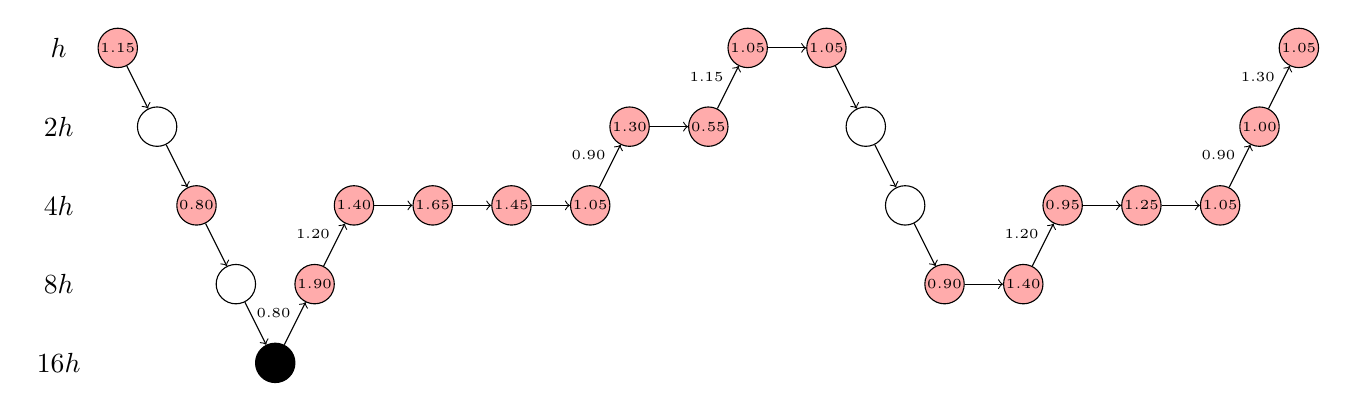
\begin{tikzpicture}
				\node   (h) at (-0.75, 4){$h$};
				\node   (2h) at (-0.75, 3){$2h$};
				\node   (4h) at (-0.75, 2){$4h$};
				\node   (8h) at (-0.75, 1){$8h$};
				\node   (16h) at (-0.75, 0){$16h$};
				\node	(a) at (0,4) [draw, fill=lightred, circle,inner sep=0pt,minimum size=5mm] {\tiny $1.15$};
				\node	(b) at (0.5,3) [draw, circle,inner sep=0pt,minimum size=5mm] {\phantom{\tiny $1.00$}};
				\node	(c) at (1,2) [draw, circle,fill=lightred,inner sep=0pt,minimum size=5mm] {\tiny $0.80$};
				\node	(d) at (1.5,1) [draw, circle,inner sep=0pt,minimum size=5mm] {\phantom{\tiny $1.00$}};
				\node	(e) at (2,0) [draw, circle,fill=black, inner sep=0pt,minimum size=5mm] {\phantom{\tiny $1.00$}};
				\node	(f) at (2.5,1) [draw, circle,  fill=lightred,inner sep=0pt,minimum size=5mm] {\tiny $1.90$};
				\node	(g) at (3,2) [draw, circle,fill=lightred,inner sep=0pt,minimum size=5mm] {\tiny $1.40$};
				\node	(h) at (4,2) [draw, circle,fill=lightred,inner sep=0pt,minimum size=5mm] {\tiny $1.65$};
				\node	(i) at (5,2) [draw, circle,fill=lightred,inner sep=0pt,minimum size=5mm] {\tiny $1.45$};
				\node	(j) at (6,2) [draw, circle,fill=lightred,inner sep=0pt,minimum size=5mm] {\tiny $1.05$};
				\node	(k) at (6.5,3) [draw, circle,fill=lightred,inner sep=0pt,minimum size=5mm] {\tiny $1.30$};
				\node	(l) at (7.5,3) [draw, circle,fill=lightred,inner sep=0pt,minimum size=5mm] {\tiny $0.55$};
				\node	(m) at (8,4) [draw, circle,fill=lightred,inner sep=0pt,minimum size=5mm] {\tiny $1.05$};
				\node	(n) at (9,4) [draw, circle,fill=lightred,inner sep=0pt,minimum size=5mm] {\tiny $1.05$};
				\node	(o) at (9.5,3) [draw, circle, inner sep=0pt,minimum size=5mm] {\phantom{\tiny $1.00$}};
				\node	(p) at (10,2) [draw, circle, inner sep=0pt,minimum size=5mm] {\phantom{\tiny $1.00$}};
				\node	(q) at (10.5,1) [draw, circle, fill=lightred, inner sep=0pt,minimum size=5mm] {\tiny $0.90$};
				\node	(r) at (11.5,1) [draw, circle, fill=lightred, inner sep=0pt,minimum size=5mm] {\tiny $1.40$};
				\node	(s) at (12,2) [draw, circle, fill=lightred, inner sep=0pt,minimum size=5mm] {\tiny $0.95$};
				\node	(t) at (13,2) [draw, circle, fill=lightred, inner sep=0pt,minimum size=5mm] {\tiny $1.25$};
				\node	(u) at (14,2) [draw, circle, fill=lightred, inner sep=0pt,minimum size=5mm] {\tiny $1.05$};
				\node	(v) at (14.5,3) [draw, circle, fill=lightred, inner sep=0pt,minimum size=5mm] {\tiny $1.00$};
				\node	(w) at (15,4) [draw, circle, fill=lightred, inner sep=0pt,minimum size=5mm] {\tiny $1.05$};
				\draw 
				(a) edge[->] (b) 
				(b) edge[->] (c)
				(c) edge[->] (d)
				(d) edge[->] (e)   
				(e) edge[->] node[near end,left] {\tiny 0.80} (f)
				(f) edge[->] node[near end,left] {\tiny 1.20} (g)
				(g) edge[->] (h)
				(h) edge[->] (i)
				(i) edge[->] (j) 
				(j) edge[->] node[near end,left] {\tiny 0.90} (k)
				(k) edge[->] (l)
				(l) edge[->] node[near end,left] {\tiny 1.15} (m)   
				(m) edge[->] (n)
				(n) edge[->] (o)
				(o) edge[->] (p)
				(p) edge[->] (q)
				(q) edge[->] (r)
				(r) edge[->] node[near end,left] {\tiny 1.20} (s)
				(s) edge[->] (t)
				(t) edge[->] (u)
				(u) edge[->] node[near end,left] {\tiny 0.90} (v)
				(v) edge[->] node[near end,left] {\tiny 1.30} (w)
				;
			\end{tikzpicture}
		}
	\caption{2D Poisson: ES-10}
	\label{fig:evolved-methods-graphical-representation:2D}
	\end{subfigure}
	\begin{subfigure}[t]{\columnwidth}
	\scalebox{0.75}{%
		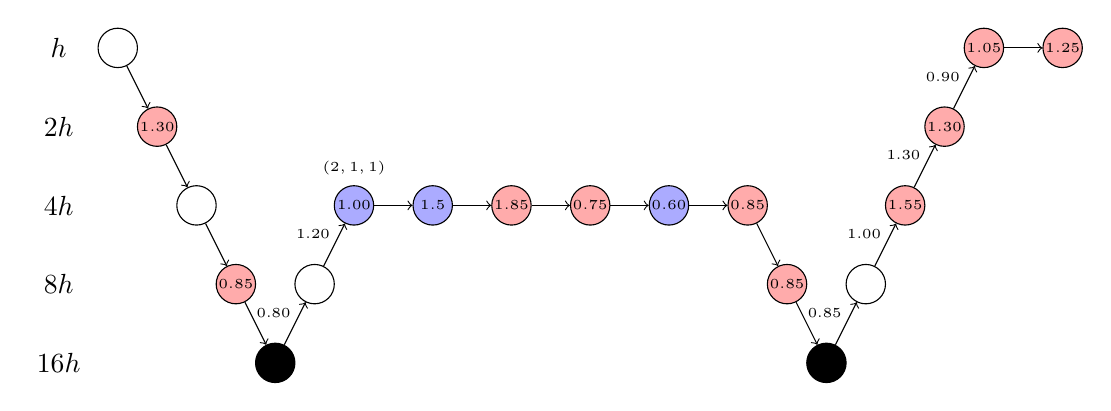
\begin{tikzpicture}
			\node   (h) at (-0.75, 4){$h$};
			\node   (2h) at (-0.75, 3){$2h$};
			\node   (4h) at (-0.75, 2){$4h$};
			\node   (8h) at (-0.75, 1){$8h$};
			\node   (16h) at (-0.75, 0){$16h$};
			\node	(a) at (0,4) [draw, circle,inner sep=0pt,minimum size=5mm] {\phantom{\tiny $1.00$}};
			\node	(b) at (0.5,3) [draw, circle, fill=lightred, inner sep=0pt,minimum size=5mm] {\tiny $1.30$};
			\node	(c) at (1,2) [draw, circle,inner sep=0pt,minimum size=5mm] {\phantom{\tiny $1.00$}};
			\node	(d) at (1.5,1) [draw, circle,fill=lightred, inner sep=0pt,minimum size=5mm] {\tiny $0.85$};
			\node	(e) at (2,0) [draw, circle,fill=black, inner sep=0pt,minimum size=5mm] {\phantom{\tiny $1.00$}};
			\node	(f) at (2.5,1) [draw, circle,inner sep=0pt,minimum size=5mm] {\phantom{\tiny $1.00$}};
			\node	(g) at (3,2) [draw, circle,fill=lightblue,inner sep=0pt,minimum size=5mm, label=above:{\tiny $(2,1,1)$}] {\tiny 1.00}; %TODO add block info
			\node	(h) at (4,2) [draw, circle,fill=lightblue,inner sep=0pt,minimum size=5mm] {\tiny $1.5$};
			\node	(i) at (5,2) [draw, circle,fill=lightred,inner sep=0pt,minimum size=5mm] {\tiny $1.85$};
			\node	(j) at (6,2) [draw, circle,fill=lightred,inner sep=0pt,minimum size=5mm] {\tiny $0.75$};
			\node	(k) at (7,2) [draw, circle,fill=lightblue,inner sep=0pt,minimum size=5mm] {\tiny $0.60$};
			\node	(l) at (8,2) [draw, circle,fill=lightred,inner sep=0pt,minimum size=5mm] {\tiny $0.85$};
			\node	(m) at (8.5,1) [draw, circle,fill=lightred,inner sep=0pt,minimum size=5mm] {\tiny $0.85$};
			\node	(n) at (9,0) [draw, circle,fill=black,inner sep=0pt,minimum size=5mm] {\phantom{\tiny $1.00$}};
			\node	(o) at (9.5,1) [draw, circle,inner sep=0pt,minimum size=5mm] {\phantom{\tiny $1.00$}};
			\node	(p) at (10,2) [draw, circle,  fill=lightred, inner sep=0pt,minimum size=5mm] {\tiny $1.55$};
			\node	(q) at (10.5,3) [draw, circle, fill=lightred, inner sep=0pt,minimum size=5mm] {\tiny $1.30$};
			\node	(r) at (11,4) [draw, circle, fill=lightred, inner sep=0pt,minimum size=5mm] {\tiny $1.05$};
			\node	(s) at (12,4) [draw, circle, fill=lightred, inner sep=0pt,minimum size=5mm] {\tiny $1.25$};
			\draw 
			(a) edge[->] (b) 
			(b) edge[->] (c)
			(c) edge[->] (d)
			(d) edge[->] (e)   
			(e) edge[->] node[near end,left] {\tiny 0.80} (f)
			(f) edge[->] node[near end,left] {\tiny 1.20} (g)
			(g) edge[->] (h)
			(h) edge[->] (i)
			(i) edge[->] (j) 
			(j) edge[->] (k)
			(k) edge[->] (l)
			(l) edge[->] (m)   
			(m) edge[->] (n)
			(n) edge[->] node[near end,left] {\tiny 0.85}(o)
			(o) edge[->] node[near end,left] {\tiny 1.00}(p)
			(p) edge[->] node[near end,left] {\tiny 1.30}(q)
			(q) edge[->] node[near end,left] {\tiny 0.90}(r)
			(r) edge[->] (s)
			;
		\end{tikzpicture}
	}
	\caption{3D Poisson: ES-9}
	\label{fig:evolved-methods-graphical-representation:3D}
	\end{subfigure}
	\caption{Computational structure of the evolved multigrid methods. The color of the node denotes the type of operation. Black: Coarse-grid solver, Blue: Block Jacobi smoothing, Red: Red-black Gauss-Seidel smoothing, White: No operation. The relaxation factor of each smoothing step is included in each node, while for coarse-grid correction, it is attached to the respective edge. For block smoothers the dimension of the block is specified on top of the respective node. If no block size is specified, a pointwise smoothing is applied.}
	\label{fig:evolved-methods-graphical-representation}
\end{figure}
The first observation that can be made from investigating the computational structure of these methods, is that none of them can be easily characterized as a V-, F- or W-cycle.
It is, therefore, impossible to formulate within the framework of classical multigrid cycles, as shown in Algorithm~\ref{alg:multigrid-cycle}.
While, for instance, the first part of Figure~\ref{fig:evolved-methods-graphical-representation:2D} can be characterized as a V-cycle, the method then proceeds with an additional coarse-grid correction step that is based on a purely smoothing-based error reduction on the coarser levels.
Figure~\ref{fig:evolved-methods-graphical-representation:3D} starts of in a similar fashion, but then applies an additional three-grid V-cycle on the third-finest level with a step size of $4h$, before it transfers the computed correction back to the finest level.
Furthermore, both evolved multigrid methods employ a different number of smoothings steps on each level using a wide range of different relaxation factors, whereby, in general, on certain levels significantly more smoothing is performed than on others.
In particular, in both cases, smoothing on the third-finest level seems to be exceptionally effective in reducing the most significant error components, and, hence, the number of smoothing steps on this level is higher than on any other level within both methods.
While both methods predominantly employ red-black Gauss-Seidel as a smoother, Figure~\ref{fig:evolved-methods-graphical-representation:3D} also includes individual pointwise and block Jacobi steps.
Finally, the complicated computational structure of the methods evolved for the linear elastic boundary prevents us from including their graphical representations similar to Figure~\ref{fig:evolved-methods-graphical-representation}.
However, if we consider the evolved method ES-2, which leads to the fastest solving time for the larger instance of the linear elastic boundary value problem with $l_{max} = 11$, we can observe a number of structural similarities with the methods shown in Figure~\ref{fig:evolved-methods-graphical-representation}.
In particular, the method applies the coarse-grid solver only once within its computations and, therefore, resembles a V-cycle, but also includes additional smoothing-based coarse-grid correction steps with a varying amount of smoothing on each level.
Furthermore, with the exception of a single Jacobi step on the second-coarsest level, the method employs exclusively red-black Gauss-Seidel smoothing.
\section{Evolving Generalizable Multigrid-Based Preconditioners for the Helmholtz Equation}
While within the last section, we could already demonstrate that our grammar-based approach leads to the automated discovery of multigrid methods with competitive performance compared to common multigrid cycles, none of the PDEs considered is particularly challenging to solve.   
Therefore, in order to evaluate whether our approach can achieve any advantages compared to state-of-the-art methods in case of such a PDE, we consider the indefinite Helmholtz equation.
At this point, we would like to point out that all results presented in this section have been originally published in~\cite{schmitt2022evolving}.
The Helmholtz equation, whose basic form is given as 
\begin{equation}
	-\nabla ^{2}u - k^{2}u = f,
	\label{eq:helmholtz}
\end{equation} 
is a famously-difficult test problem for the application of numerical methods, that also has practical relevance for many real-world applications, such as~\cite{versteeg1994marmousi,martin2006marmousi2,billette20052004,gray1995migration}.
The main difficulty in solving this equation is that the system of linear equations resulting from its discretization becomes highly ill-conditioned for large values of the wavenumber $k$~\cite{ernst2012difficult}.
If we, for instance, assume the use of ten grid points per wavelength~\footnote{Usually the relation of the wavelength $\lambda$ to the wavenumber $k$ is defined as $k = \frac{2 \pi}{\lambda}$ }, as it is common in geophysical applications~\cite{erlangga2006multigrid}, on the dimensionless unit square, a second-order accuracy requirement of $kh = 0.625$ must be fulfilled.
Figure~\ref{fig:condition-number-helmholtz} shows the condition number of the system matrix $A$ that results from a discretization of Equation~\eqref{eq:helmholtz} for different values of the wavenumber $k$.
\begin{figure}
		\centering
		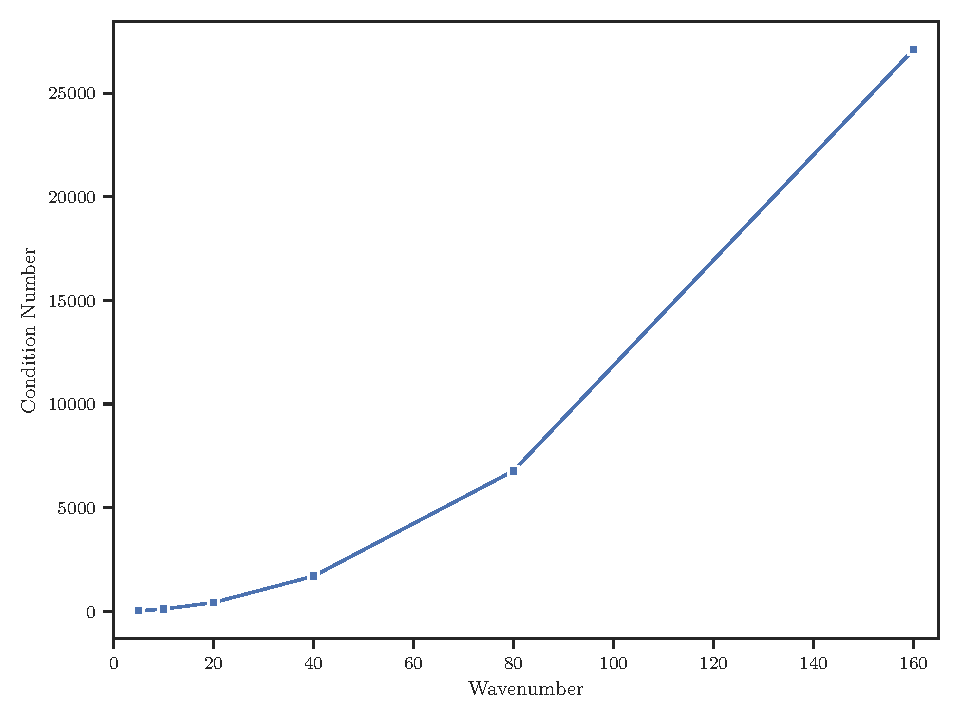
\includegraphics[width=\textwidth]{figures/cond.pdf}
		\caption{Condition number of the system matrix resulting from a finite-difference discretization of the two-dimensional Helmholtz equation with $kh = 0.625$}
		\label{fig:condition-number-helmholtz}
\end{figure}
The condition number gives us a notion of how much an initial approximation error is magnified by the application of the operator $A$.
As we can see in Figure~\ref{fig:condition-number-helmholtz} for larger values of $k$ the condition number of $A$ increases dramatically, which results in an extreme accumulation of numerical errors. 
Therefore, the necessity to handle these errors makes the design of an efficient or even functioning numerical method for the indefinite Helmholtz equation outstandingly difficult.
In particular, without any modification classical multigrid methods can not effectively be applied as a numerical solver for indefinite Helmholtz problems~\cite{ernst2012difficult}.
One multigrid-based approach that mitigates this problem is the application of multigrid as a preconditioner instead of applying it to the discretized Helmholtz system directly.
In general, preconditioning has the purpose of modifying a given system of linear equations, by applying a so-called preconditioning matrix $M$ in order to obtain a new system that is then easier to solve.
For instance, right-preconditioning the system $A x = b$ with the matrix $M$ results in
\begin{equation}
	A M^{-1} \bm{y} = \bm{b},
	\label{eq:right-preconditioning}
\end{equation}
with $M \bm{x} = \bm{y}$. 
The main consequence of this formulation is that, we now have to solve an additional system of linear equations of the form of $M \bm{x} = \bm{y}$, whenever the operator $A$ is applied within our original solution method.
If we consider the extreme choice of $M$ as the original operator $A$, this means that Equation~\eqref{eq:right-preconditioning} reduces to $I \bm{y} = \bm{b}$, however with the consequence that the system $M \bm{x} = \bm{y}$ becomes just as ill-conditioned as the original one.
Therefore, the choice of the preconditioning matrix $M$ usually represents a compromise between the accurate approximation of the original matrix $A$ to effectively improve its condition number and the ease of solveability of $M \bm{x} = \bm{y}$~\cite{benzi2002preconditioning}.
In the recent decades the choice of $M$ as a complex-shifted version of the original operator, has proven its effectiveness for indefinite Helmholtz problems~\cite{erlangga2004preconditioner,erlangga2008advances,cocquet2017shift}, which leads to
\begin{equation*}
	M = -\nabla ^{2} - (k^{2} + i \varepsilon).
\end{equation*}
%TODO include all suitable citations
As it has been shown in~\cite{cocquet2017shift}, a shift $\varepsilon \approx \mathcal{O}(k^2)$ enables the efficient inversion of $M$ by multigrid, whereas the choice of a smaller shift increases the preconditioning effectiveness.
Since the resulting linear system $A M^{-1} \bm{y} = \bm{b}$ is complex-symmetric but non-hermitian, it is then commonly solved using a suitable Krylov subspace method, such as GMRES and BiCGSTAB~\cite{saad2003iterative}.
\subsection{Problem Formulation}
After introducing the indefinite Helmholtz equation and the difficulties its solution comprises in general manner, we can now proceed by defining a representative instance of this equation for the evaluation of our grammar-based approach for multigrid method design.
For this purpose, we consider the two-dimensional Helmholtz equation on a unit square with Dirichlet boundary conditions at the top and bottom, and Robin radiation conditions at the left and right, as given by
\begin{equation}
	\label{eq:helmholtz-test-problem}
	\begin{split}
		(-\nabla ^{2} - k^{2}) u & = f \quad \text{in} \; \left( 0, 1 \right)^2 \\
		u & = 0 \quad \text{on} \; \left( 0, 1 \right) \times \{0\}, \left( 0, 1 \right) \times \{1\} \\
		\partial_{\mathbf{n}} u - iku & = 0 \quad \text{on} \; \{0\} \times \left( 0, 1 \right), \{1\} \times \left( 0, 1 \right) \\
		f(x, y) & = \delta(x - 0.5, y - 0.5),
	\end{split}
\end{equation}
where $\delta(\bm{x})$ is the Dirac delta function.
We discretize this equation on a uniform Cartesian grid using the classical five-point stencil
\begin{equation*}
	A_h = \frac{1}{h^2} \begin{bmatrix}
		& -1 & \\
		-1 & 4 - (k h)^2 & -1 \\
		& -1 &  
	\end{bmatrix}.
\end{equation*}
In addition, $\delta(\bm{x})$ is approximated with a second-order Zenger correction~\cite{koestler2004extrapolation}.
The spacing $h$ of the grid is chosen to fulfill the second-order accuracy requirement $h k = 0.625$ as described above.
Finally, the shifted-Laplacian
\begin{equation*}
	M = -\nabla^{2} - (k^{2} + 0.5 i k^{2}),
\end{equation*}
which is discretized similar to the original operator using the five-point stencil
\begin{equation*}
	M_h = \frac{1}{h^2} \begin{bmatrix}
		& -1 & \\
		-1 & 4 - (1.0 + 0.5i)(k h)^2 & -1 \\
		& -1 &  
	\end{bmatrix}.
\end{equation*}
\subsection{Solver Configuration}
As a result of the above formulation of our test problem, we obtain two systems of linear equations
\begin{equation}
	A_h M_h^{-1} \bm{y}_h = \bm{b}_h,
	\label{eq:helmholtz-test-problem-discretized-and-preconditioned}
\end{equation}
where $\bm{b}_h$ contains the values of $\delta(\bm{x})$ at each grid point, and
\begin{equation}
	M_h \bm{x}_h = \bm{y}_h,
	\label{eq:helmholtz-test-problem-preconditioning}
\end{equation}
where $\bm{x}$ represents the approximate solution of Equation~\eqref{eq:helmholtz-test-problem}.
While for each of these two systems of linear equations, a functioning solver is needed, the focus of our experimental evaluation is the design of an efficient multigrid method for the approximate solution of Equation~\eqref{eq:helmholtz-test-problem-preconditioning}.
Here, to limit the cost of preconditioning, we assume that the application of a single multigrid cycle is sufficient to compute a reasonable approximation for $M_{h}^{-1}$.
After obtaining a suitable multigrid-based preconditioner, Equation~\ref{eq:helmholtz-test-problem-discretized-and-preconditioned} is then solved using the a biconjugate gradient stabilized method (BiCGSTAB)~\cite{saad2003iterative}.
The resulting iterative solution scheme is shown in Algorithm~\ref{alg:preconditioned-bicgstab}, in which, for the sake of simplicity, omit the grid spacing $h$.
\begin{algorithm}[t]
	\caption{Right-Preconditioned BiCGSTAB}
	\label{alg:preconditioned-bicgstab}
	\begin{algorithmic}[1] % The number tells where the line numbering should start
			\State $\bm{r}^0 = \bm{b} - A \bm{x}^0$
			\State $\bm{\hat{r}}^0 = \bm{r}^0$
			\State $\alpha_0 = \beta_0 = \rho_0 = \omega_0 = 1$
			\State $\bm{p}^0 = \bm{q}^0 = \bm{0}$
			\For{$i := 1, \dots, n$}
			\State $\rho_i = \bm{\hat{r}}^{i-1} \cdot \bm{r}^{i-1}$
			\State $\beta_i = \frac{\rho_i }{\rho_{i-1} }\frac{\alpha_{i-1}}{ \omega_{i-1}}$
			\State $\bm{p}^i = \bm{r}^{i-1} + \beta_i (\bm{p}^{i-1} - \omega_{i-1} \bm{q}^{i-1})$
			\State Solve $M \bm{x}^i = \bm{p}^i$
			\State $\bm{q}^i = A \bm{x}^i$
			\State $\alpha_i = \rho_i / (\bm{\hat{r}}^{i-1} \cdot \bm{q}^i)$
			\State $\bm{h}^i = \bm{x}^{i-1} + \alpha_i \bm{x}^i$	
			\State $\bm{s}^i = \bm{r}^{i-1} - \alpha_i \bm{r}^i$
			\State Solve $M \bm{x}^i = \bm{s}^i$
			\State $\bm{t}^i = A \bm{x}^i$
			\State $\omega_i = (\bm{t}^i \cdot \bm{s}^i) / (\bm{t}^i \cdot \bm{t}^i)$
			\State $\bm{x}^i = \bm{h}^i + \omega_i \bm{x}^i$
			\State $\bm{r}^i = \bm{s}^i - \omega_i \bm{t}^i$
			\If{$\norm{\bm{r}^i}/\norm{\bm{r}^0} < \epsilon$}
			\Return $\bm{x}^i$
			\EndIf
			\EndFor
		\end{algorithmic}
\end{algorithm}
In each step of this iterative scheme, it is necessary to compute an approximate solution for two systems of linear equations of the form $M \bm{x}^i = \bm{y}^i$, %, in line 9 and 14, 
each of which is then achieved through the application of a single multigrid cycle.
To construct an efficient method for this purpose, we consider the set of five-grid methods that are defined on a hierarchy of discretization with $h = 1/2^{l}$ on each level $l \in \left[l_{max} - 4,l_{max}\right]$. 
Similar to Section~\ref{sec:experiments-part1}, we then consider the following components within each step of the method:
\begin{description}
	\item[\textbf{Smoothers}:] Pointwise and block Jacobi with rectangular blocks up to a maximum number of six terms, red-black Gauss-Seidel
	\item[\textbf{Restriction}:] Full-weighting restriction
	\item[\textbf{Prolongation}:] Bilinear interpolation
	\item[\textbf{Relaxation factors}:] $\left( 0.1 + 0.05i \right)_{i = 0}^{36} = \left(0.1, 0.15, 0.2, \dots, 1.9 \right)$
	\item[\textbf{Coarse-grid solver}:] BiCGSTAB for $l = l_{max} - 4$
\end{description}
The resulting grammar is similar to the multigrid grammar shown in Figure~\ref{table:multigrid-grammar}, however, with the modification that each occurrence of a system matrix $A_H$ and right-hand side $\ps{b_H}$ is replaced by the respective preconditioning matrix $M_H$ and right-hand side $\ps{y_H}$.
Similar to Section~\ref{sec:experiments1-multigrid-configuration}, block Jacobi smoothers are generated based on rectangular blocks of grid points, while the relaxation factor $\omega$ of each smoothing and coarse-grid correction step is chosen from the above interval.
To assess the efficiency and generalizability of the multigrid preconditioners evolved with our approach, we consider the set of possible multigrid cycles that can be constructed based on the classical formulation of these methods, using the same components as described above, for comparison.
In order to ensure, that these methods represent the state of the art we ensure to pick the optimal smoother and relaxation factor for the given case, which is determined by evaluating each possible combination from the available set of options on the largest problem size for which we convergence can be achieved.
Due to the ill-conditioning of the indefinite Helmholtz equation, we consider an approximate solution to be sufficient, when the initial residual has been reduced by a factor of $10^{-7}$ for $k \leq 160$ and $10^{-6}$ for all larger wavenumbers.

\section{Optimization Settings and Evaluation Platform}
In Section~\ref{sec:experiments-part1}, the relative simplicity of the problems considered along with the fact that our main focus has been to gain an understanding of the general behavior of our evolutionary algorithm, motivates use to keep the problem size constant during each optimization run.
However, in the given case this strategy is infeasible due to a number of reasons.
First of all, doubling the wavenumber requires us to use twice as many grid points in each dimension because of the requirement $kh = 0.625$, which means that we end up with a system of linear equations that is not only significantly worse conditioned, but also has four times the number of unknowns.
As a consequence, solving Helmholtz problems with large wavenumber becomes tremendously expensive, which makes the evaluation of a large number of different preconditioners infeasible.
Furthermore, in practice, our goal is to evolve multigrid methods that can be applied to a wide range of different problem instances and, thus, generalizability is one of our main concerns.
In Section~\ref{sec:generalization-procedure}, we have already proposed a systematic procedure for the generalization of a population of individuals to a set of instances of the same problem.
This method aims to evolve a population of generalizable multigrid methods by iteratively increasing the size of the test problem considered within the evaluation of each solver after a certain number of generations $m$.
While the formulation of our problem based on the wavenumber-dependent grid spacing $h$ allows us to construct problem instances of larger size and difficulty in a straightforward manner, it is unclear after how many generations this operation should be performed.
However, in the experiments performed in Section~\ref{sec:experiments-part1} we could observe that the majority of improvement in both objectives is achieved within the first 50 generations of each optimization run.
Therefore, setting the generalization interval $m$ to 50 represents a reasonable compromise between allowing the population to adapt to modified conditions and preventing it from overfitting to the characteristics of a particular problem instance.
To initiate each optimization run, we choose $k = 80$ as a problem instance, which leads to a maximum level $l_{max} = 7$ and a system of linear equations consisting of 16129 unknowns. 
Therefore, the cost of evaluation at the beginning of the search is drastically reduced compared to later generations.
We then execute Algorithm~\ref{alg:generalization-procedure} with a population size of 128 and a total number of 150 generations, whereby after 50 and 100 generations we increase the value of wavenumber to 160 and 320, respectively.
In order to evaluate each multigrid method obtained during the search, we utilize it as a preconditioner within Algorithm~\ref{alg:preconditioned-bicgstab}, as described above.
Note that while population size as well as the number of generations is smaller than within our experimental evaluation in Section~\ref{sec:experiments-part1}, the time required to evaluate each solver drastically increases for larger wavenumbers, leading to an overall higher computational cost for each optimization run.
Similar to Section~\ref{sec:experiments-part1} we perform a total number of ten experiments, each of which is executed on SuperMUC-NG\footnote{SuperMUC-NG: \url{https://doku.lrz.de/display/PUBLIC/SuperMUC-NG}}.
To parallelize our evolutionary search method, we rely on the distributed parallel described in Section~\ref{sec:distributed-parallelization} using 64 MPI processes that are distributed to eight compute nodes of the system, where each process is exclusively executed on one of the eight available islands.
Therefore, each process creates and evaluates two new individuals per generation, which are then evaluated on the respective island using on OpenMP-based shared-memory parallelization with 12 threads.
\chapter{Related Work and Conclusion}
  %\section{Comparison with Related Work}
In the last chapter, we could demonstrate that our evolutionary program synthesis approach leads to the discovery of multigrid methods with novel algorithmic features.
By applying the generalization procedure presented in  Section~\ref{sec:generalization}, we were able to evolve multigrid methods that yield a high degree of efficiency in solving different instances of the same discretized PDE, one of them being intractable using classical multigrid methods.
However, since the application of artificial intelligence (AI) and automated algorithm design to the solution of PDEs includes a wide range of different methods, it is important to classify the approach presented here within this quickly growing field.
% In contrast to other %TODO provide more explanation
% We can classify AI-based methods for solving PDEs according to different criteria.
Figure~\ref{fig:overview-ai-based-methods} gives an overview of the state of AI-based methods for solving PDEs at the time this thesis was published.
\begin{figure}
	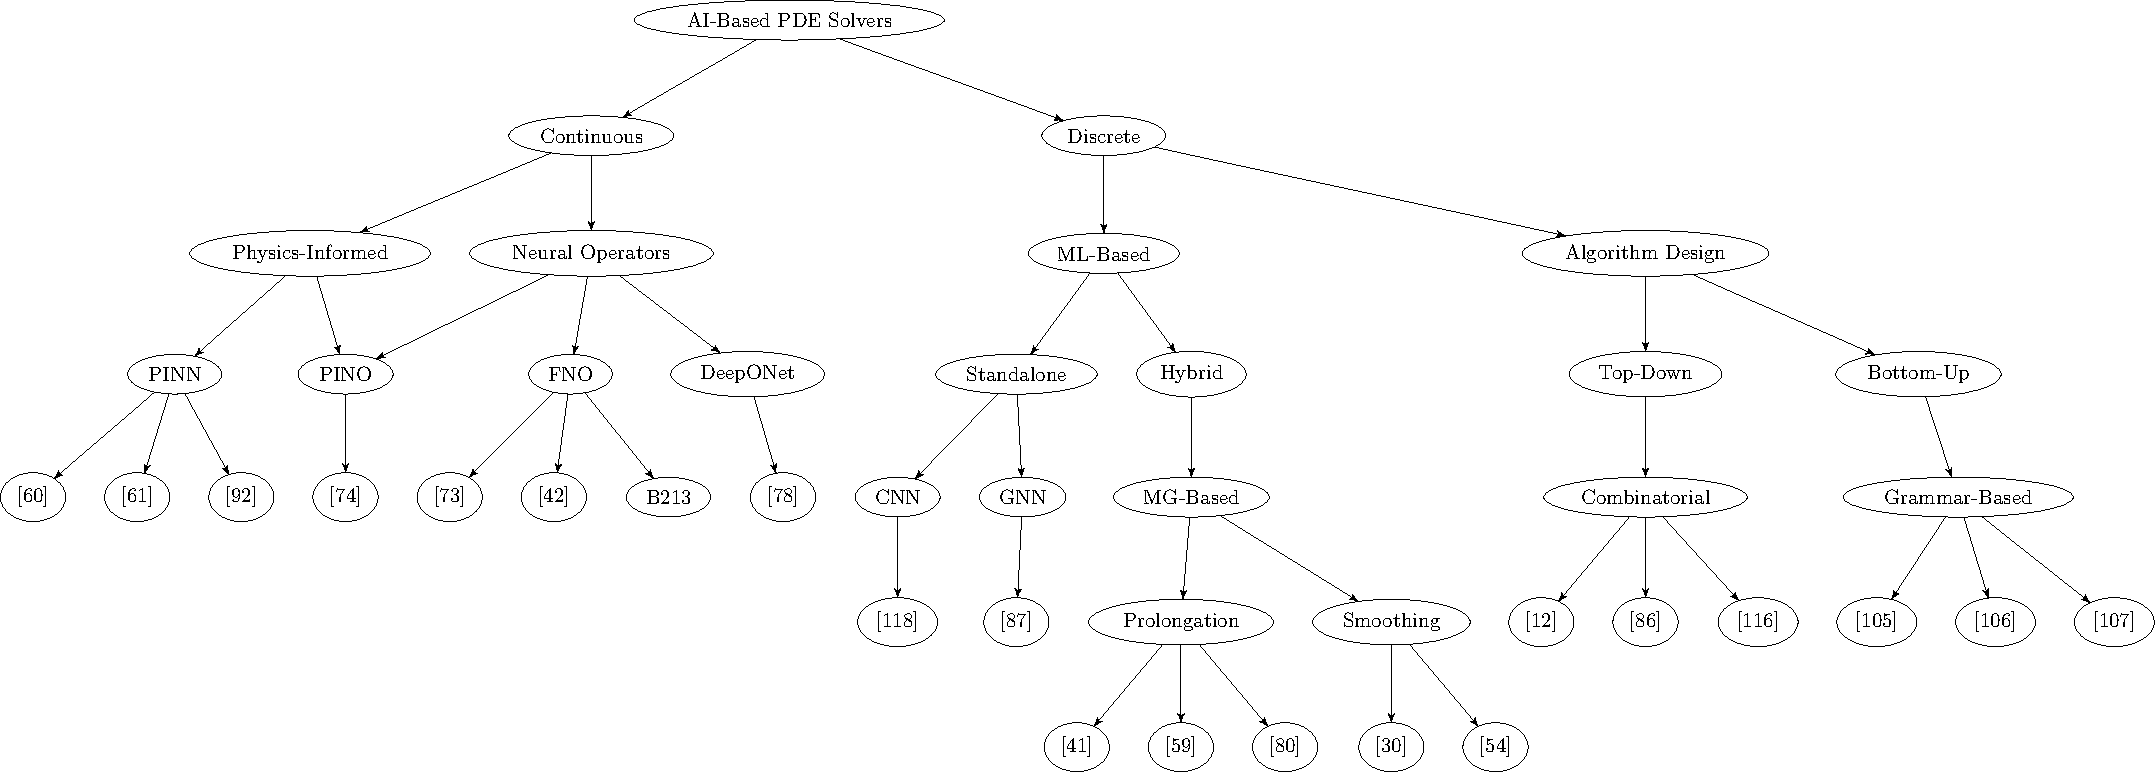
\includegraphics[width=\textwidth]{figures/trees/related_work.pdf}
	\caption{Overview of AI-based methods for solving PDEs. Each leaf node represents a different class of method presented in at least one research paper.}
	\label{fig:overview-ai-based-methods}
\end{figure}
First of all, we can distinguish methods that aim to solve a PDE directly in the continuous domain and those that require it to be formulated as a discrete problem, usually obtained by applying a specific discretization method.
The currently most popular~\footnote{Here, we consider the number of citations as a popularity metric.} methods based on machine learning (ML), physics-informed neural networks~\cite{karniadakis2021physics,raissi2019physics,kharazmi2019variational,kharazmi2021hp} and neural operators~\cite{li2020fourier,guibas2021efficient,lu2021learning,li2021physics} fall into the former category.
This class of methods aims to approximate the function that represents the solution or the operator of a given PDE by exploiting the fact that neural networks can act as universal function approximators when given enough data~\cite{hornik1989multilayer}.
Physics-informed methods try to improve over purely data-driven methods by directly incorporating the physical constraints of the given PDE into the learning process.
Neural operators aim to achieve a higher degree of generalization by learning a representation of the operator of a PDE instead of approximating its solution.
Recently, the usability of ML-based methods has been tremendously improved through the availability of easy-to-use and well-maintained implementations, such as DeepXDE~\cite{lu2021deepxde} and NVIDIA Modulus~\cite{hennigh2021nvidia}. 
Instead of directly targeting a PDE in the continuous domain, the second branch of AI-based methods operates on its discrete version, obtained after applying a suitable discretization method.
Therefore, these methods can either act as a direct replacement for classical numerical solvers or operate in combination with them.
An early example of the former is the neural network-based PDE solver proposed by Lagaris et al.~\cite{lagaris1998artificial} but also more recent approaches based on convolutional~\cite{thuerey2020deep} and graph neural networks~\cite{pfaff2020learning} fall into this category.
In contrast, AI-based methods that work in combination with existing solvers do not try to replace the method as a whole but rather aim to enhance it, for instance, by adding or replacing certain steps of the method or by finding an optimal configuration for each of its parameters and design options.
Multigrid methods are an often-considered target since these methods have the potential to achieve an optimal asymptotic complexity while possessing a large number of configuration options and complex interactions between each of their components.
A first step towards the automated design of multigrid methods has been the work by Oosterlee and Wienands~\cite{oosterlee2003genetic}, which uses a genetic algorithm to optimize the choice of each multigrid component.
Similarly, Thekale et al.~\cite{thekale2010optimizing} aim to optimize the number of multigrid cycles within a full-multigrid method using a branch-and-bound approach, while Brown et al.~\cite{brown2021tuning} optimize the algorithmic parameters of a two-grid method by solving a minimax problem obtained from an LFA-based analysis.
All these works have in common that they are based on the classical formulation of multigrid methods, as shown in Algorithm~\ref{alg:multigrid-cycle}.
Since the resulting optimization capabilities are still restricted to a set of global parameters, these approaches can be classified as top-down algorithm design or algorithm configuration methods.
In contrast, as we have shown in this work, expressing each possible computational step of a multigrid method as a separate production within a context-free grammar allows treating the task of designing an optimal multigrid method as a program synthesis problem.
%Therefore, according to our classification of algorithm design methods in Chapter~%TODO insert ref her
Therefore, together with this thesis, the papers~\cite{schmitt2020constructing,schmitt2021evostencils,schmitt2022evolving} can be considered the first implementation of a bottom-up approach for the automated design of multigrid methods.
However, while our approach offers the flexibility to construct arbitrary sequences of multigrid operations on a given hierarchy of discretizations, similar to~\cite{oosterlee2003genetic,thekale2010optimizing,brown2021tuning}, we consider the internal structure of each individual operation as immutable.
Recently, ML-based approaches have been utilized to enhance or replace certain operations within a multigrid method.
A first example is the works by Katrutsa et al.~\cite{katrutsa2020black}, Greenfeld et al.~\cite{greenfeld2019learning}, and Luz et at.~\cite{luz2020learning}, which utilizes ML to discover optimized prolongation operators.
Huang et al.~\cite{huang2021learning}, and Fanaskov~\cite{fanaskov2021neural} apply a similar approach to the optimization of smoothers.
The works by Taghibakhshi et al.~\cite{taghibakhshi2021optimization}, and Markidis~\cite{markidis2021old} go even one step further.
In the former, the authors replace the coarsening step within an algebraic multigrid method altogether with an ML system, while in~\cite{markidis2021old}, the author proposes to employ a physics-informed neural network as a coarse-grid solver.
Finally, Hsieh et al.~\cite{hsieh2019learning} take a different direction by enhancing the approximation obtained in each step of an iterative solver with an additional neural network-based correction.
Since these approaches all focus on the optimization of the individual components of a multigrid method but consider the method's algorithmic structure as immutable, they can be considered as a complementary approach to the algorithm design methods discussed earlier in this section.
However, a combination of both paradigms has not yet been considered and could be a promising research direction for the future.
One possibility to achieve this goal would be to incorporate learned operators or even ML-based methods that act as a replacement for certain solver components into the search space of a top-down or bottom-up algorithm design method.
%We will discuss this possibility together with other potential extensions of our approach in the following final section of this thesis.

  \paragraph{Conclusion}
We have started this thesis with an introduction to automated algorithm design methods and their successful application to different domains.
Since our main goal was to harness the potential of these methods for the automated design of multigrid methods for solving partial differential equations (PDEs), the question of whether we have achieved our original goals remains to be answered.
After establishing a theoretical foundation on multigrid methods, formal languages, and evolutionary program synthesis, in Chapter~\ref{chapter:multigrid-formal-language}, we have derived a novel context-free grammar, which enables us to construct sequences of multigrid operations that could not yet be obtained with the classical formulation of these methods.
Building upon this foundation, we have then presented a prototypical implementation of our evolutionary program synthesis tool, called \emph{EvoStencils}, which automates the design and implementation of efficient and generalizable multigrid-based PDE solvers by leveraging the capabilities of the evolutionary computation library DEAP~\cite{rainville2012deap} and the ExaStencils~\cite{lengauer2020exastencils} code generation framework.
In Chapter~\ref{chapter:experiments}, we were then able to demonstrate that this approach yields efficient multigrid methods for different PDEs, whereby using the example of the indefinite Helmholtz equation, our automatically-designed solvers were even able to achieve super-human performance in an outstandingly-difficult benchmark problem for the application of numerical PDE solvers\footnote{For this result, the corresponding paper has been awarded the 2022 Humies Gold Award for Human-Competitive Results (\url{https://www.human-competitive.org/awards})}.
While we believe that this lays the foundation for the utilization of automated algorithm design methods within the domain of numerical PDE solvers, these multigrid methods only represent a tiny fraction of this vast research area.
%We, therefore, believe that there exists a multitude of promising extensions of this work, some of which we briefly want to discuss in the following.
Therefore, a promising extension of this work is the application of the presented approach to other multigrid variants or even other classes of numerical solvers.
While this thesis, as a starting point, focuses on classical geometric multigrid methods, since the invention of these methods, several other variants have been developed which are tailored to other use cases.
One example is the full-approximation scheme (FAS), which can be considered a non-linear version of multigrid~\cite{trottenberg2000multigrid,briggs2000multigrid}.
While the formulation of the FAS method requires replacing both the smoother and coarse-grid solver with non-linear variants that are often based on Newton's or Picard's method, the application of our evolutionary program synthesis requires only a minimal amount of adaption.
To illustrate this, Section~\ref{appendix:fas} shows the necessary adaptions of our original state transition functions and grammar productions for generating FAS-style multigrid methods. 
As it can be seen there, apart from updating the respective productions, essentially only the two functions \textsc{cycle} and \textsc{cgc} need to be changed, while we additionally provide a new state transition function \textsc{cgs} for the application of the coarse-grid solver. 
Note that since, in the case of FAS, the application of the operator $A_h$ no longer represents a linear operation, we instead denote it as a function application.
Another promising extension would be an extension of our approach to full-multigrid (FMG) methods.
While in Section~\ref{sec:experiments-part1}, we have demonstrated that multigrid cycles designed with our approach represent faster solvers than common multigrid cycles for different PDEs, in many cases, including Poisson's equation, FMG represents the fastest and most efficient available solver for linear problems~\cite{trottenberg2000multigrid}.
Since FMG is based on the application of multigrid cycles on different levels of a given discretization hierarchy, one possibility would be to apply our evolutionary program synthesis method to each of these individual cycles.
While this approach would lead to an even larger search space than the ones considered in this work, it could yield methods that achieve even higher efficiency in solving PDE-based problems.
Finally, another class of multigrid methods not yet considered in this work is algebraic multigrid (AMG).
In contrast to geometric multigrid, AMG methods derive all of their operations directly from an algebraic formulation of a system of linear equations in the form of a (usually sparse) matrix.
While this makes these methods fundamentally different from the multigrid methods considered in this work, the actual algorithmic structure of AMG methods is no different from their geometric counterparts.
We could, therefore, formulate a grammar structurally similar to the one shown in Table~\ref{table:multigrid-grammar} that simply replaces each individual operation applied within their productions with their algebraic equivalent, which would allow us to utilize the same program synthesis approach for the automated design of AMG methods.
Another direction of extension would be to target the current limitations in the evaluation accuracy of the predictive models briefly discussed in Section~\ref{sec:fitness-evaluation-and-selection}.
While local Fourier analysis (LFA) has been successfully applied to different applications, the missing availability of broadly-tested open-source tools for its automated use currently limits its applicability to the approach presented here.
In case this situation might not change in the future, one alternative would be to instead use a statistical model to predict the quality of a certain multigrid method based on a history of samples.
One popular approach to mitigate the issue of needing to perform a large number of costly evaluations, which has proven to be successful in other domains of automated algorithm design such as automated machine learning (AutoML), is Bayesian optimization (BO).%TODO include ref

\appendix 
  %%% WRITE YOUR APPENDIX DIRECTLY HERE OR %%%%%%%%
  %%% INPUT AN EXTERNAL FILE WITH YOUR APPENDIX %%%
\section{Intermediate Representation}
\label{appendix:ir}
\begin{listing}[!htb]
	\inputminted{python}{evostencils/ir/inter_grid_operator.py}
	\caption{IR: Inter-Grid Operator Base Class}
	\label{code:ir:inter-grid-operator}
\end{listing}
\begin{listing}[!htb]
	\inputminted{python}{evostencils/ir/restriction.py}
	\caption{IR: Restriction}
	\label{code:ir:restriction}
\end{listing}
\begin{listing}[!htb]
	\inputminted{python}{evostencils/ir/prolongation.py}
	\caption{IR: Prolongation}
	\label{code:ir:prolongation}
\end{listing}
\begin{listing}[!htb]
	\inputminted{python}{evostencils/ir/diagonal.py}
	\caption{IR: Diagonal and Block-Diagonal}
	\label{code:ir:diagonal}
\end{listing}
\begin{listing}[!htb]
	\inputminted{python}{evostencils/ir/multiplication.py}
	\caption{IR: Operator Application}
	\label{code:ir:multiplication}
\end{listing}
\clearpage
\section{Genetic Programming}
\label{appendix:gp}
\begin{listing}[!htb]
	\inputminted{python}{evostencils/gp/primitive_set_typed.py}
	\caption{PrimitiveSetTyped}
	\label{code:gp:primitive-set-typed}
\end{listing}
\begin{listing}[!htb]
	\inputminted{python}{evostencils/gp/generate.py}
	\caption{Tree generation function}
	\label{code:gp:generate}
\end{listing}
\clearpage
\section{Full-Approximation Scheme (FAS)}
\label{appendix:fas}

\begin{bnf}
\setcounter{equation}{6}
\bnfprod{$s_{h}$} {
	\bnfts{\textnormal{\textsc{update}}}(\bnfts{$\omega$}, \bnfsp \bnfes, \bnfsp \bnfts{\textnormal{\textsc{cgc}}}(\bnfts{$I_{2h}^{h}$}, \bnfts{$I_{h}^{2h}$}, \bnfsp \bnfpn{$s_{2h}$}))
 }
 \\
\setcounter{equation}{8}
\bnfprod{$s_{2h}$} {
    \bnfts{\textnormal{\textsc{cgs}}}(\bnfts{$I_{4h}^{2h}$}, \bnfsp \bnfts{$A_{4h}$}, \bnfsp \bnfts{$I_{2h}^{4h}$}, \bnfpn{$s_{2h}$})
	}
 \\
 \setcounter{equation}{11}
\bnfprod{$c_{2h}$} {
	\bnfts{\textnormal{\textsc{cycle}}}(\bnfts{$A_{2h}$}, \bnfsp \bnfts{$x^0_{2h}$}, \bnfsp \bnfts{\textnormal{\textsc{apply}}}(\bnfts{$I_h^{2h}$}, \bnfsp \bnfpn{$c_h$}))
}
\end{bnf}
\begin{table}[!htb]
	%\caption{State transition functions adapted for FAS}
	%\label{table:fas-grammar-semantics}
	\begin{algorithmic}
	\Function{cycle}{$A_{2h}$, $x_{2h}^0$, $I_{h}^{2h}$, ($\tilde{x}_h$, $b_{h}$, $c_{2h}$, $S_{h/2}$)}
	\State $\tilde{x}_{2h} \gets x_{2h}^0$ 
	\State $b_{2h} \gets c_{2h} + A_{2h} \left( I_{h}^{2h} \tilde{x}_h \right) $
	\State $c_{2h} \gets b_{2h} - A_{2h} \left( \tilde{x}_{2h} \right)$ 
	\State $S_h \gets$ ($\tilde{x}_{h}$, $b_{h}$, $\lambda$, $S_{h/2}$)
	\State return ($\tilde{x}_{2h}$, $b_{2h}$, $c_{2h}$, $S_h$)
	\EndFunction
	\State
	\Function{cgc}{$I_{2h}^{h}$, $I_{h}^{2h}$, $(\tilde{x}_{2h}, b_{2h}, \lambda, S_{h})$}
	\State ($\tilde{x}_h$, $f_{h}$, $c_h$, $S_{h/2}$) $\gets S_{h}$
	\State $c_h \gets I_{2h}^{h} \cdot (\tilde{x}_{2h} - I_{h}^{2h} \tilde{x}_h)$
	\State return ($\tilde{x}_h$, $f_{h}$, $c_h$, $S_{h/2}$)
	\EndFunction
    \State
	\Function{cgs}{$I_{2h}^{h}$, $A_{2h}$, $I_{h}^{2h}$, ($\tilde{x}_h$, $b_{h}$, $c_{h}$, $S_{h/2}$)}
	\State $x_{h} \gets I_{2h}^{h} \left( A_{2h}^{-1}\left( I_{h}^{2h} c_h \right) - I_{h}^{2h} \tilde{x}_h \right)$ 
	\State return ($\tilde{x}_{h}$, $b_{h}$, $c_{h}$, $S_{h/2}$)
	\EndFunction
	\end{algorithmic}
\end{table}

% start the backmatter (arabic page numbering [continued],
% no sectioning numbering, header)
\backmatter
  \faupressprintbibliography
   \faupressprintacronyms
  \begingroup
  \listofalgorithms
  \let\clearpage\relax
  \listoflistings
  \endgroup

\end{document}
